\chapter{Calibration of the ProtoDUNE detector}
\label{sec:pdune_calibration}

\section{Lifetime measurements}
\label{sec:pdune_calibration:lifetime}

In this chapter electron lifetime measurements from two sources are presented.
The first of these measurements comes from the purity monitors situation within the ProtoDUNE-SP cryostat (see \citesec{sec:protodune:prms}).

The second of these measurements utilises the high rate of cosmic rays impinging upon the detector.
These cosmic rays have a well known and roughly constant energy deposition before they stop.
This constant energy deposition means that they can be used as a `standard candle' throughout the TPC.
As a result, any observed changes in the energy deposition as a function of position within the detector must result from detector non-uniformities.
In particular, measured changes in the charge deposition as a function of drift distance can be used to measure the electron lifetime.

This measurement is attempted and presented in \citesec{sec:pdune_calibration:lifetime:selection}.

\subsection{Particle selection}
\label{sec:pdune_calibration:lifetime:selection}

In order to make an accurate measurement of the electron lifetime, it is important to ensure that those particles which are selected have the desired constant energy profile.
Typically, particles generate one of two types of structure in a LAr TPC.

High energy electrons and photons typically generate structures termed `showers' when they strike a high density material such as liquid argon.
In the case of electrons, these showers develop due to the emission of photons by the electron from bremsstrahlung.
These photons then produce further $e^{+}e^{-}$ pairs of lower energy via pair production and the process continues until the energy of the remaining photons falls below the threshold required for pair production.
A similar process occurs for photons but without the initial bremsstrahlung phase.
An image of a typical electromagnetic shower in a LAr TPC is shown in \citefigL{fig:trackShower}.
One can see that the energy deposition occurs in a rough cone shape with many branches.

Heavier particles such as proton, muons and hadrons typically produce `tracks' rather than showers.
This is due to their larger mass which inhibits radiative energy losses such as bremsstrahlung.
Instead they typically produce linear energy depositions until either scattering or coming to rest.
A typical image of a track recorded in ProtoDUNE-SP is shown in \citefigR{fig:trackShower}.
These tracks have an energy deposition that is more easily measured than that of showers.

\begin{figure}[h]
	\begin{minipage}[t]{.49\linewidth}
		\includegraphics[width=\linewidth]{files/figures/protodune_calibration/showerCand}
	\end{minipage}
	\hfill
	\begin{minipage}[t]{.49\linewidth}
		\includegraphics[width=\linewidth]{files/figures/protodune_calibration/trackCand}		
	\end{minipage}
	\caption[Images of typical track and shower structures in ProtoDUNE-SP]{Left: Image of a \SI{0.5}{\GeV\per\clight} electron candidate in ProtoDUNE-SP, showing typical shower structure, from~\cite{protodunePerformance}. Right: Image of a \SI{1}{\GeV\per\clight} stopping proton candidate in ProtoDUNE-SP, showing typical track structure, from~\cite{protodunePerformance}.}
	\label{fig:trackShower}
\end{figure}

As shown in \citefig{fig:energyLoss}, as charged particles reach lower momenta their energy loss grows.
Therefore, it is desirable to only select those particles that are not in this region of rapidly changing energy deposition.
Specifically, it is desirable to only select those particles in the minimum ionising region of the energy loss profile.

\citefigL{fig:muonEDep}, shows the relationship between a muon's residual range and its average \dedx in liquid argon.
The average energy loss is calculated here using the `Bethe' formula~\cite{pdg2018} which gives the energy energy loss for a particle of charge $z$, mass $M$ and with a velocity $v$ such that $\beta = \frac{v}{c}$ and $\gamma = 1 / \sqrt{1 - \beta^{2}}$:
\begin{equation}
	\left< -\frac{dE}{dx} \right> = K z^{2} \rho \frac{Z}{A} \frac{1}{\beta^{2}} 
	\left[ \frac{1}{2} \ln \frac{2m_{e}c^{2} \beta^{2} \gamma^{2} W_{\text{max}}}{I^{2}} - \beta^{2} - \frac{\delta (\beta \gamma)}{2} \right] \, .
\end{equation}
Here, $Z$, $A$, $\rho$ and $I$ are the atomic number, relative atomic mass, density and mean excitation energy of the target medium.
$m_{e}$ is the electron rest mass and $K$ is equal to \SI{0.307075}{\MeV\per\mole\square\cm}.
The term $\delta(\beta\gamma)$ is known as the density-effect correction and is computed using a parametrisation from~\cite{densityEffect}.
$W_{\text{max}}$ is the maximum energy transferred to an electron in a single collision and is equal to 
\begin{equation}
	W_{\text{max}} =  \frac{ 2 m_{e} c^{2} \beta^{2} \gamma^{2} }{ 1 + 2\gamma m_{e}/M + (m_{e}/M)^{2} } \, .
\end{equation}
One can see that, at residual range of $>\SI{50}{\cm}$ there is little change in the energy loss with increasing range.

\citefigR{fig:muonEDep} shows the variation in the calculated most probable value (MPV) of energy loss for a muon in liquid argon as a function of muon kinetic energy.
Here one can see, that even at energies of up to \SI{100}{\GeV} the muon energy loss remains roughly constant compared to the minimum.
The most probable energy loss is calculated using the formula~\cite{mpvELoss}
\begin{equation}
	\Delta_{p} = \xi \left[ \ln \frac{2m_{e}c^{2} \beta^{2} \gamma^{2}}{I^{2}} +
	\ln \frac{\xi}{I} + j - \beta^{2} - \delta(\beta\gamma) \right] \, ,
\end{equation}
where 
\begin{equation}
	\xi = \left( \frac{K}{2} \right) \left< \frac{Z}{A} \right> z^{2} \left( \frac{x\rho}{\beta^{2}} \right)~\text{MeV}
\end{equation}
and $x$ is the thickness of the material (here \SI{0.65}{\cm} is chosen).

\begin{figure}[h]
	\begin{minipage}[t]{.5\linewidth}
		\begin{adjustbox}{max totalsize=\linewidth, center}
			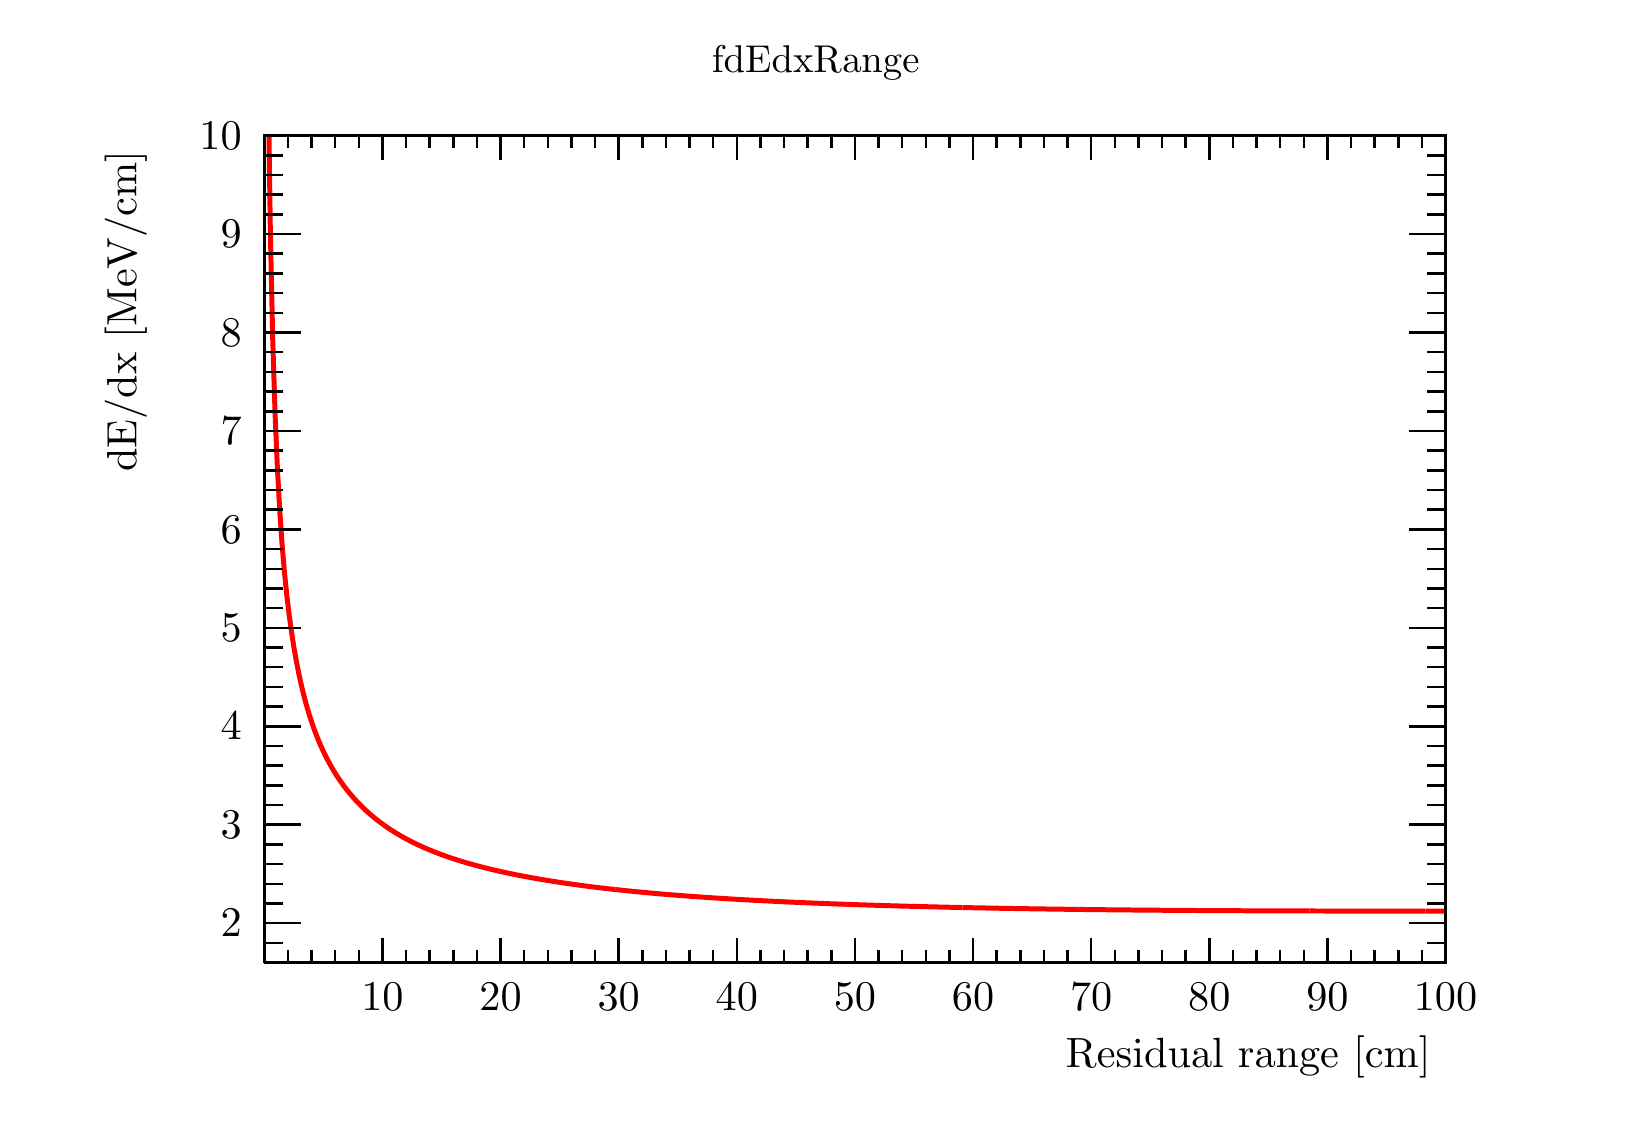
\begin{tikzpicture}
\pgfdeclareplotmark{cross} {
\pgfpathmoveto{\pgfpoint{-0.3\pgfplotmarksize}{\pgfplotmarksize}}
\pgfpathlineto{\pgfpoint{+0.3\pgfplotmarksize}{\pgfplotmarksize}}
\pgfpathlineto{\pgfpoint{+0.3\pgfplotmarksize}{0.3\pgfplotmarksize}}
\pgfpathlineto{\pgfpoint{+1\pgfplotmarksize}{0.3\pgfplotmarksize}}
\pgfpathlineto{\pgfpoint{+1\pgfplotmarksize}{-0.3\pgfplotmarksize}}
\pgfpathlineto{\pgfpoint{+0.3\pgfplotmarksize}{-0.3\pgfplotmarksize}}
\pgfpathlineto{\pgfpoint{+0.3\pgfplotmarksize}{-1.\pgfplotmarksize}}
\pgfpathlineto{\pgfpoint{-0.3\pgfplotmarksize}{-1.\pgfplotmarksize}}
\pgfpathlineto{\pgfpoint{-0.3\pgfplotmarksize}{-0.3\pgfplotmarksize}}
\pgfpathlineto{\pgfpoint{-1.\pgfplotmarksize}{-0.3\pgfplotmarksize}}
\pgfpathlineto{\pgfpoint{-1.\pgfplotmarksize}{0.3\pgfplotmarksize}}
\pgfpathlineto{\pgfpoint{-0.3\pgfplotmarksize}{0.3\pgfplotmarksize}}
\pgfpathclose
\pgfusepathqstroke
}
\pgfdeclareplotmark{cross*} {
\pgfpathmoveto{\pgfpoint{-0.3\pgfplotmarksize}{\pgfplotmarksize}}
\pgfpathlineto{\pgfpoint{+0.3\pgfplotmarksize}{\pgfplotmarksize}}
\pgfpathlineto{\pgfpoint{+0.3\pgfplotmarksize}{0.3\pgfplotmarksize}}
\pgfpathlineto{\pgfpoint{+1\pgfplotmarksize}{0.3\pgfplotmarksize}}
\pgfpathlineto{\pgfpoint{+1\pgfplotmarksize}{-0.3\pgfplotmarksize}}
\pgfpathlineto{\pgfpoint{+0.3\pgfplotmarksize}{-0.3\pgfplotmarksize}}
\pgfpathlineto{\pgfpoint{+0.3\pgfplotmarksize}{-1.\pgfplotmarksize}}
\pgfpathlineto{\pgfpoint{-0.3\pgfplotmarksize}{-1.\pgfplotmarksize}}
\pgfpathlineto{\pgfpoint{-0.3\pgfplotmarksize}{-0.3\pgfplotmarksize}}
\pgfpathlineto{\pgfpoint{-1.\pgfplotmarksize}{-0.3\pgfplotmarksize}}
\pgfpathlineto{\pgfpoint{-1.\pgfplotmarksize}{0.3\pgfplotmarksize}}
\pgfpathlineto{\pgfpoint{-0.3\pgfplotmarksize}{0.3\pgfplotmarksize}}
\pgfpathclose
\pgfusepathqfillstroke
}
\pgfdeclareplotmark{newstar} {
\pgfpathmoveto{\pgfqpoint{0pt}{\pgfplotmarksize}}
\pgfpathlineto{\pgfqpointpolar{44}{0.5\pgfplotmarksize}}
\pgfpathlineto{\pgfqpointpolar{18}{\pgfplotmarksize}}
\pgfpathlineto{\pgfqpointpolar{-20}{0.5\pgfplotmarksize}}
\pgfpathlineto{\pgfqpointpolar{-54}{\pgfplotmarksize}}
\pgfpathlineto{\pgfqpointpolar{-90}{0.5\pgfplotmarksize}}
\pgfpathlineto{\pgfqpointpolar{234}{\pgfplotmarksize}}
\pgfpathlineto{\pgfqpointpolar{198}{0.5\pgfplotmarksize}}
\pgfpathlineto{\pgfqpointpolar{162}{\pgfplotmarksize}}
\pgfpathlineto{\pgfqpointpolar{134}{0.5\pgfplotmarksize}}
\pgfpathclose
\pgfusepathqstroke
}
\pgfdeclareplotmark{newstar*} {
\pgfpathmoveto{\pgfqpoint{0pt}{\pgfplotmarksize}}
\pgfpathlineto{\pgfqpointpolar{44}{0.5\pgfplotmarksize}}
\pgfpathlineto{\pgfqpointpolar{18}{\pgfplotmarksize}}
\pgfpathlineto{\pgfqpointpolar{-20}{0.5\pgfplotmarksize}}
\pgfpathlineto{\pgfqpointpolar{-54}{\pgfplotmarksize}}
\pgfpathlineto{\pgfqpointpolar{-90}{0.5\pgfplotmarksize}}
\pgfpathlineto{\pgfqpointpolar{234}{\pgfplotmarksize}}
\pgfpathlineto{\pgfqpointpolar{198}{0.5\pgfplotmarksize}}
\pgfpathlineto{\pgfqpointpolar{162}{\pgfplotmarksize}}
\pgfpathlineto{\pgfqpointpolar{134}{0.5\pgfplotmarksize}}
\pgfpathclose
\pgfusepathqfillstroke
}
\definecolor{c}{rgb}{1,1,1};
\draw [color=c, fill=c] (0,0) rectangle (20,13.639);
\draw [color=c, fill=c] (3,1.77307) rectangle (18,12.2751);
\definecolor{c}{rgb}{0,0,0};
\draw [c,line width=0.9] (3,1.77307) -- (3,12.2751) -- (18,12.2751) -- (18,1.77307) -- (3,1.77307);
\definecolor{c}{rgb}{1,1,1};
\draw [color=c, fill=c] (3,1.77307) rectangle (18,12.2751);
\definecolor{c}{rgb}{0,0,0};
\draw [c,line width=0.9] (3,1.77307) -- (3,12.2751) -- (18,12.2751) -- (18,1.77307) -- (3,1.77307);
\definecolor{c}{rgb}{1,0,0};
\draw [c,line width=1.8] (3.05761,12.2751) -- (3.075,11.0517);
\draw [c,line width=1.8] (3.075,11.0517) -- (3.105,9.69138) -- (3.135,8.74094) -- (3.165,8.03897) -- (3.195,7.49881) -- (3.225,7.06959) -- (3.255,6.71937) -- (3.285,6.42706) -- (3.315,6.17811) -- (3.345,5.96213) -- (3.375,5.77157) -- (3.405,5.60162)
 -- (3.435,5.44905) -- (3.465,5.31128) -- (3.495,5.18619) -- (3.525,5.07206) -- (3.555,4.96743) -- (3.585,4.87111) -- (3.615,4.78206) -- (3.645,4.69943) -- (3.675,4.62245) -- (3.705,4.5505) -- (3.735,4.48303) -- (3.765,4.4196) -- (3.795,4.35985) --
 (3.825,4.30345) -- (3.855,4.25011) -- (3.885,4.19956) -- (3.915,4.15159) -- (3.945,4.10598) -- (3.975,4.06255) -- (4.005,4.02111) -- (4.035,3.98153) -- (4.065,3.94366) -- (4.095,3.90737) -- (4.125,3.87256) -- (4.155,3.83911) -- (4.185,3.80694) --
 (4.215,3.77598) -- (4.245,3.74616) -- (4.275,3.71743) -- (4.305,3.68973) -- (4.335,3.663) -- (4.365,3.63719) -- (4.395,3.61227) -- (4.425,3.58818) -- (4.455,3.56488) -- (4.485,3.54234) -- (4.515,3.52053);
\draw [c,line width=1.8] (4.515,3.52053) -- (4.545,3.4994) -- (4.575,3.47893) -- (4.605,3.45908) -- (4.635,3.43984) -- (4.665,3.42117) -- (4.695,3.40305) -- (4.725,3.38545) -- (4.755,3.36835) -- (4.785,3.35174) -- (4.815,3.33559) -- (4.845,3.31988)
 -- (4.875,3.3046) -- (4.905,3.28973) -- (4.935,3.27524) -- (4.965,3.26114) -- (4.995,3.2474) -- (5.025,3.23401) -- (5.055,3.22095) -- (5.085,3.20822) -- (5.115,3.1958) -- (5.145,3.18367) -- (5.175,3.17184) -- (5.205,3.16029) -- (5.235,3.149) --
 (5.265,3.13798) -- (5.295,3.12721) -- (5.325,3.11667) -- (5.355,3.10637) -- (5.385,3.0963) -- (5.415,3.08645) -- (5.445,3.07681) -- (5.475,3.06737) -- (5.505,3.05813) -- (5.535,3.04908) -- (5.565,3.04021) -- (5.595,3.03153) -- (5.625,3.02301) --
 (5.655,3.01467) -- (5.685,3.00649) -- (5.715,2.99846) -- (5.745,2.99059) -- (5.775,2.98287) -- (5.805,2.97529) -- (5.835,2.96786) -- (5.865,2.96055) -- (5.895,2.95338) -- (5.925,2.94634) -- (5.955,2.93942) -- (5.985,2.93262);
\draw [c,line width=1.8] (5.985,2.93262) -- (6.015,2.92594) -- (6.045,2.91937) -- (6.075,2.91291) -- (6.105,2.90656) -- (6.135,2.90032) -- (6.165,2.89417) -- (6.195,2.88813) -- (6.225,2.88218) -- (6.255,2.87632) -- (6.285,2.87056) -- (6.315,2.86488)
 -- (6.345,2.8593) -- (6.375,2.85379) -- (6.405,2.84837) -- (6.435,2.84303) -- (6.465,2.83777) -- (6.495,2.83259) -- (6.525,2.82748) -- (6.555,2.82245) -- (6.585,2.81749) -- (6.615,2.81261) -- (6.645,2.8078) -- (6.675,2.80306) -- (6.705,2.79838) --
 (6.735,2.79377) -- (6.765,2.78923) -- (6.795,2.78476) -- (6.825,2.78034) -- (6.855,2.776) -- (6.885,2.77171) -- (6.915,2.76748) -- (6.945,2.76331) -- (6.975,2.7592) -- (7.005,2.75515) -- (7.035,2.75115) -- (7.065,2.74721) -- (7.095,2.74332) --
 (7.125,2.73948) -- (7.155,2.7357) -- (7.185,2.73197) -- (7.215,2.72829) -- (7.245,2.72466) -- (7.275,2.72108) -- (7.305,2.71755) -- (7.335,2.71406) -- (7.365,2.71062) -- (7.395,2.70723) -- (7.425,2.70388) -- (7.455,2.70058);
\draw [c,line width=1.8] (7.455,2.70058) -- (7.485,2.69732) -- (7.515,2.6941) -- (7.545,2.69092) -- (7.575,2.68779) -- (7.605,2.6847) -- (7.635,2.68164) -- (7.665,2.67863) -- (7.695,2.67565) -- (7.725,2.67272) -- (7.755,2.66982) -- (7.785,2.66696) --
 (7.815,2.66413) -- (7.845,2.66134) -- (7.875,2.65858) -- (7.905,2.65586) -- (7.935,2.65318) -- (7.965,2.65053) -- (7.995,2.64791) -- (8.025,2.64532) -- (8.055,2.64276) -- (8.085,2.64024) -- (8.115,2.63775) -- (8.145,2.63528) -- (8.175,2.63285) --
 (8.205,2.63045) -- (8.235,2.62807) -- (8.265,2.62573) -- (8.295,2.62341) -- (8.325,2.62112) -- (8.355,2.61886) -- (8.385,2.61662) -- (8.415,2.61441) -- (8.445,2.61223) -- (8.475,2.61008) -- (8.505,2.60794) -- (8.535,2.60584) -- (8.565,2.60376) --
 (8.595,2.6017) -- (8.625,2.59967) -- (8.655,2.59766) -- (8.685,2.59567) -- (8.715,2.59371) -- (8.745,2.59177) -- (8.775,2.58985) -- (8.805,2.58795) -- (8.835,2.58608) -- (8.865,2.58422) -- (8.895,2.58239) -- (8.925,2.58058);
\draw [c,line width=1.8] (8.925,2.58058) -- (8.955,2.57879) -- (8.985,2.57702) -- (9.015,2.57527) -- (9.045,2.57354) -- (9.075,2.57182) -- (9.105,2.57013) -- (9.135,2.56846) -- (9.165,2.5668) -- (9.195,2.56517) -- (9.225,2.56355) -- (9.255,2.56195)
 -- (9.285,2.56036) -- (9.315,2.5588) -- (9.345,2.55725) -- (9.375,2.55572) -- (9.405,2.5542) -- (9.435,2.5527) -- (9.465,2.55122) -- (9.495,2.54975) -- (9.525,2.5483) -- (9.555,2.54687) -- (9.585,2.54545) -- (9.615,2.54405) -- (9.645,2.54266) --
 (9.675,2.54129) -- (9.705,2.53993) -- (9.735,2.53858) -- (9.765,2.53725) -- (9.795,2.53594) -- (9.825,2.53463) -- (9.855,2.53335) -- (9.885,2.53207) -- (9.915,2.53081) -- (9.945,2.52956) -- (9.975,2.52833) -- (10.005,2.52711) -- (10.035,2.5259) --
 (10.065,2.5247) -- (10.095,2.52352) -- (10.125,2.52235) -- (10.155,2.52119) -- (10.185,2.52005) -- (10.215,2.51891) -- (10.245,2.51779) -- (10.275,2.51668) -- (10.305,2.51558) -- (10.335,2.51449) -- (10.365,2.51342) -- (10.395,2.51235);
\draw [c,line width=1.8] (10.395,2.51235) -- (10.425,2.5113) -- (10.455,2.51025) -- (10.485,2.50922) -- (10.515,2.5082) -- (10.545,2.50719) -- (10.575,2.50619) -- (10.605,2.5052) -- (10.635,2.50422) -- (10.665,2.50325) -- (10.695,2.50229) --
 (10.725,2.50134) -- (10.755,2.5004) -- (10.785,2.49947) -- (10.815,2.49855) -- (10.845,2.49764) -- (10.875,2.49674) -- (10.905,2.49584) -- (10.935,2.49496) -- (10.965,2.49409) -- (10.995,2.49322) -- (11.025,2.49237) -- (11.055,2.49152) --
 (11.085,2.49068) -- (11.115,2.48986) -- (11.145,2.48903) -- (11.175,2.48822) -- (11.205,2.48742) -- (11.235,2.48662) -- (11.265,2.48584) -- (11.295,2.48506) -- (11.325,2.48429) -- (11.355,2.48353) -- (11.385,2.48277) -- (11.415,2.48203) --
 (11.445,2.48129) -- (11.475,2.48056) -- (11.505,2.47983) -- (11.535,2.47912) -- (11.565,2.47841) -- (11.595,2.47771) -- (11.625,2.47701) -- (11.655,2.47633) -- (11.685,2.47565) -- (11.715,2.47498) -- (11.745,2.47431) -- (11.775,2.47366) --
 (11.805,2.473) -- (11.835,2.47236) -- (11.865,2.47172);
\draw [c,line width=1.8] (11.865,2.47172) -- (11.895,2.47109) -- (11.925,2.47047) -- (11.955,2.46985) -- (11.985,2.46924) -- (12.015,2.46864) -- (12.045,2.46804) -- (12.075,2.46745) -- (12.105,2.46687) -- (12.135,2.46629) -- (12.165,2.46572) --
 (12.195,2.46515) -- (12.225,2.46459) -- (12.255,2.46404) -- (12.285,2.46349) -- (12.315,2.46295) -- (12.345,2.46241) -- (12.375,2.46188) -- (12.405,2.46135) -- (12.435,2.46084) -- (12.465,2.46032) -- (12.495,2.45982) -- (12.525,2.45931) --
 (12.555,2.45882) -- (12.585,2.45833) -- (12.615,2.45784) -- (12.645,2.45736) -- (12.675,2.45689) -- (12.705,2.45642) -- (12.735,2.45595) -- (12.765,2.45549) -- (12.795,2.45504) -- (12.825,2.45459) -- (12.855,2.45414) -- (12.885,2.45371) --
 (12.915,2.45327) -- (12.945,2.45284) -- (12.975,2.45242) -- (13.005,2.452) -- (13.035,2.45158) -- (13.065,2.45117) -- (13.095,2.45077) -- (13.125,2.45037) -- (13.155,2.44997) -- (13.185,2.44958) -- (13.215,2.44919) -- (13.245,2.44881) --
 (13.275,2.44843) -- (13.305,2.44806) -- (13.335,2.44769);
\draw [c,line width=1.8] (13.335,2.44769) -- (13.365,2.44733) -- (13.395,2.44697) -- (13.425,2.44661) -- (13.455,2.44626) -- (13.485,2.44591) -- (13.515,2.44557) -- (13.545,2.44523) -- (13.575,2.44489) -- (13.605,2.44456) -- (13.635,2.44423) --
 (13.665,2.44391) -- (13.695,2.44359) -- (13.725,2.44328) -- (13.755,2.44297) -- (13.785,2.44266) -- (13.815,2.44235) -- (13.845,2.44205) -- (13.875,2.44176) -- (13.905,2.44147) -- (13.935,2.44118) -- (13.965,2.44089) -- (13.995,2.44061) --
 (14.025,2.44033) -- (14.055,2.44006) -- (14.085,2.43979) -- (14.115,2.43952) -- (14.145,2.43926) -- (14.175,2.439) -- (14.205,2.43874) -- (14.235,2.43849) -- (14.265,2.43824) -- (14.295,2.43799) -- (14.325,2.43775) -- (14.355,2.43751) --
 (14.385,2.43727) -- (14.415,2.43704) -- (14.445,2.43681) -- (14.475,2.43658) -- (14.505,2.43636) -- (14.535,2.43614) -- (14.565,2.43592) -- (14.595,2.43571) -- (14.625,2.4355) -- (14.655,2.43529) -- (14.685,2.43508) -- (14.715,2.43488) --
 (14.745,2.43468) -- (14.775,2.43449) -- (14.805,2.43429);
\draw [c,line width=1.8] (14.805,2.43429) -- (14.835,2.4341) -- (14.865,2.43392) -- (14.895,2.43373) -- (14.925,2.43355) -- (14.955,2.43337) -- (14.985,2.4332) -- (15.015,2.43302) -- (15.045,2.43285) -- (15.075,2.43269) -- (15.105,2.43252) --
 (15.135,2.43236) -- (15.165,2.4322) -- (15.195,2.43204) -- (15.225,2.43189) -- (15.255,2.43174) -- (15.285,2.43159) -- (15.315,2.43144) -- (15.345,2.4313) -- (15.375,2.43116) -- (15.405,2.43102) -- (15.435,2.43088) -- (15.465,2.43075) --
 (15.495,2.43062) -- (15.525,2.43049) -- (15.555,2.43037) -- (15.585,2.43024) -- (15.615,2.43012) -- (15.645,2.43) -- (15.675,2.42989) -- (15.705,2.42977) -- (15.735,2.42966) -- (15.765,2.42955) -- (15.795,2.42944) -- (15.825,2.42934) --
 (15.855,2.42924) -- (15.885,2.42914) -- (15.915,2.42904) -- (15.945,2.42894) -- (15.975,2.42885) -- (16.005,2.42876) -- (16.035,2.42867) -- (16.065,2.42858) -- (16.095,2.4285) -- (16.125,2.42841) -- (16.155,2.42833) -- (16.185,2.42825) --
 (16.215,2.42818) -- (16.245,2.4281) -- (16.275,2.42803);
\draw [c,line width=1.8] (16.275,2.42803) -- (16.305,2.42796) -- (16.335,2.42789) -- (16.365,2.42782) -- (16.395,2.42776) -- (16.425,2.4277) -- (16.455,2.42764) -- (16.485,2.42758) -- (16.515,2.42752) -- (16.545,2.42747) -- (16.575,2.42741) --
 (16.605,2.42736) -- (16.635,2.42731) -- (16.665,2.42727) -- (16.695,2.42722) -- (16.725,2.42718) -- (16.755,2.42714) -- (16.785,2.4271) -- (16.815,2.42706) -- (16.845,2.42702) -- (16.875,2.42699) -- (16.905,2.42696) -- (16.935,2.42693) --
 (16.965,2.4269) -- (16.995,2.42687) -- (17.025,2.42684) -- (17.055,2.42682) -- (17.085,2.4268) -- (17.115,2.42678) -- (17.145,2.42676) -- (17.175,2.42674) -- (17.205,2.42673) -- (17.235,2.42671) -- (17.265,2.4267) -- (17.295,2.42669) --
 (17.325,2.42668) -- (17.355,2.42667) -- (17.385,2.42667) -- (17.415,2.42666) -- (17.445,2.42666) -- (17.475,2.42666) -- (17.505,2.42666) -- (17.535,2.42666) -- (17.565,2.42666) -- (17.595,2.42667) -- (17.625,2.42668) -- (17.655,2.42668) --
 (17.685,2.42669) -- (17.715,2.4267) -- (17.745,2.42672);
\draw [c,line width=1.8] (17.745,2.42672) -- (17.775,2.42673) -- (17.805,2.42674) -- (17.835,2.42676) -- (17.865,2.42678) -- (17.895,2.4268) -- (17.925,2.42682) -- (17.955,2.42684) -- (17.985,2.42686);
\definecolor{c}{rgb}{0,0,0};
\draw [c,line width=0.9] (3,1.77307) -- (18,1.77307);
\draw [c,line width=0.9] (4.49865,2.07994) -- (4.49865,1.77307);
\draw [c,line width=0.9] (4.79868,1.9265) -- (4.79868,1.77307);
\draw [c,line width=0.9] (5.09871,1.9265) -- (5.09871,1.77307);
\draw [c,line width=0.9] (5.39874,1.9265) -- (5.39874,1.77307);
\draw [c,line width=0.9] (5.69877,1.9265) -- (5.69877,1.77307);
\draw [c,line width=0.9] (5.9988,2.07994) -- (5.9988,1.77307);
\draw [c,line width=0.9] (6.29883,1.9265) -- (6.29883,1.77307);
\draw [c,line width=0.9] (6.59886,1.9265) -- (6.59886,1.77307);
\draw [c,line width=0.9] (6.89889,1.9265) -- (6.89889,1.77307);
\draw [c,line width=0.9] (7.19892,1.9265) -- (7.19892,1.77307);
\draw [c,line width=0.9] (7.49895,2.07994) -- (7.49895,1.77307);
\draw [c,line width=0.9] (7.79898,1.9265) -- (7.79898,1.77307);
\draw [c,line width=0.9] (8.09901,1.9265) -- (8.09901,1.77307);
\draw [c,line width=0.9] (8.39904,1.9265) -- (8.39904,1.77307);
\draw [c,line width=0.9] (8.69907,1.9265) -- (8.69907,1.77307);
\draw [c,line width=0.9] (8.9991,2.07994) -- (8.9991,1.77307);
\draw [c,line width=0.9] (9.29913,1.9265) -- (9.29913,1.77307);
\draw [c,line width=0.9] (9.59916,1.9265) -- (9.59916,1.77307);
\draw [c,line width=0.9] (9.89919,1.9265) -- (9.89919,1.77307);
\draw [c,line width=0.9] (10.1992,1.9265) -- (10.1992,1.77307);
\draw [c,line width=0.9] (10.4993,2.07994) -- (10.4993,1.77307);
\draw [c,line width=0.9] (10.7993,1.9265) -- (10.7993,1.77307);
\draw [c,line width=0.9] (11.0993,1.9265) -- (11.0993,1.77307);
\draw [c,line width=0.9] (11.3993,1.9265) -- (11.3993,1.77307);
\draw [c,line width=0.9] (11.6994,1.9265) -- (11.6994,1.77307);
\draw [c,line width=0.9] (11.9994,2.07994) -- (11.9994,1.77307);
\draw [c,line width=0.9] (12.2994,1.9265) -- (12.2994,1.77307);
\draw [c,line width=0.9] (12.5995,1.9265) -- (12.5995,1.77307);
\draw [c,line width=0.9] (12.8995,1.9265) -- (12.8995,1.77307);
\draw [c,line width=0.9] (13.1995,1.9265) -- (13.1995,1.77307);
\draw [c,line width=0.9] (13.4995,2.07994) -- (13.4995,1.77307);
\draw [c,line width=0.9] (13.7996,1.9265) -- (13.7996,1.77307);
\draw [c,line width=0.9] (14.0996,1.9265) -- (14.0996,1.77307);
\draw [c,line width=0.9] (14.3996,1.9265) -- (14.3996,1.77307);
\draw [c,line width=0.9] (14.6997,1.9265) -- (14.6997,1.77307);
\draw [c,line width=0.9] (14.9997,2.07994) -- (14.9997,1.77307);
\draw [c,line width=0.9] (15.2997,1.9265) -- (15.2997,1.77307);
\draw [c,line width=0.9] (15.5998,1.9265) -- (15.5998,1.77307);
\draw [c,line width=0.9] (15.8998,1.9265) -- (15.8998,1.77307);
\draw [c,line width=0.9] (16.1998,1.9265) -- (16.1998,1.77307);
\draw [c,line width=0.9] (16.4998,2.07994) -- (16.4998,1.77307);
\draw [c,line width=0.9] (16.7999,1.9265) -- (16.7999,1.77307);
\draw [c,line width=0.9] (17.0999,1.9265) -- (17.0999,1.77307);
\draw [c,line width=0.9] (17.3999,1.9265) -- (17.3999,1.77307);
\draw [c,line width=0.9] (17.7,1.9265) -- (17.7,1.77307);
\draw [c,line width=0.9] (18,2.07994) -- (18,1.77307);
\draw [c,line width=0.9] (4.49865,2.07994) -- (4.49865,1.77307);
\draw [c,line width=0.9] (4.19862,1.9265) -- (4.19862,1.77307);
\draw [c,line width=0.9] (3.89859,1.9265) -- (3.89859,1.77307);
\draw [c,line width=0.9] (3.59856,1.9265) -- (3.59856,1.77307);
\draw [c,line width=0.9] (3.29853,1.9265) -- (3.29853,1.77307);
\draw [anchor=base] (4.49865,1.15931) node[scale=1.52731, color=c, rotate=0]{10};
\draw [anchor=base] (5.9988,1.15931) node[scale=1.52731, color=c, rotate=0]{20};
\draw [anchor=base] (7.49895,1.15931) node[scale=1.52731, color=c, rotate=0]{30};
\draw [anchor=base] (8.9991,1.15931) node[scale=1.52731, color=c, rotate=0]{40};
\draw [anchor=base] (10.4993,1.15931) node[scale=1.52731, color=c, rotate=0]{50};
\draw [anchor=base] (11.9994,1.15931) node[scale=1.52731, color=c, rotate=0]{60};
\draw [anchor=base] (13.4995,1.15931) node[scale=1.52731, color=c, rotate=0]{70};
\draw [anchor=base] (14.9997,1.15931) node[scale=1.52731, color=c, rotate=0]{80};
\draw [anchor=base] (16.4998,1.15931) node[scale=1.52731, color=c, rotate=0]{90};
\draw [anchor=base] (18,1.15931) node[scale=1.52731, color=c, rotate=0]{100};
\draw [anchor= east] (18,0.572837) node[scale=1.52731, color=c, rotate=0]{Residual range [cm]};
\draw [c,line width=0.9] (3,12.2751) -- (18,12.2751);
\draw [c,line width=0.9] (4.49865,11.9682) -- (4.49865,12.2751);
\draw [c,line width=0.9] (4.79868,12.1216) -- (4.79868,12.2751);
\draw [c,line width=0.9] (5.09871,12.1216) -- (5.09871,12.2751);
\draw [c,line width=0.9] (5.39874,12.1216) -- (5.39874,12.2751);
\draw [c,line width=0.9] (5.69877,12.1216) -- (5.69877,12.2751);
\draw [c,line width=0.9] (5.9988,11.9682) -- (5.9988,12.2751);
\draw [c,line width=0.9] (6.29883,12.1216) -- (6.29883,12.2751);
\draw [c,line width=0.9] (6.59886,12.1216) -- (6.59886,12.2751);
\draw [c,line width=0.9] (6.89889,12.1216) -- (6.89889,12.2751);
\draw [c,line width=0.9] (7.19892,12.1216) -- (7.19892,12.2751);
\draw [c,line width=0.9] (7.49895,11.9682) -- (7.49895,12.2751);
\draw [c,line width=0.9] (7.79898,12.1216) -- (7.79898,12.2751);
\draw [c,line width=0.9] (8.09901,12.1216) -- (8.09901,12.2751);
\draw [c,line width=0.9] (8.39904,12.1216) -- (8.39904,12.2751);
\draw [c,line width=0.9] (8.69907,12.1216) -- (8.69907,12.2751);
\draw [c,line width=0.9] (8.9991,11.9682) -- (8.9991,12.2751);
\draw [c,line width=0.9] (9.29913,12.1216) -- (9.29913,12.2751);
\draw [c,line width=0.9] (9.59916,12.1216) -- (9.59916,12.2751);
\draw [c,line width=0.9] (9.89919,12.1216) -- (9.89919,12.2751);
\draw [c,line width=0.9] (10.1992,12.1216) -- (10.1992,12.2751);
\draw [c,line width=0.9] (10.4993,11.9682) -- (10.4993,12.2751);
\draw [c,line width=0.9] (10.7993,12.1216) -- (10.7993,12.2751);
\draw [c,line width=0.9] (11.0993,12.1216) -- (11.0993,12.2751);
\draw [c,line width=0.9] (11.3993,12.1216) -- (11.3993,12.2751);
\draw [c,line width=0.9] (11.6994,12.1216) -- (11.6994,12.2751);
\draw [c,line width=0.9] (11.9994,11.9682) -- (11.9994,12.2751);
\draw [c,line width=0.9] (12.2994,12.1216) -- (12.2994,12.2751);
\draw [c,line width=0.9] (12.5995,12.1216) -- (12.5995,12.2751);
\draw [c,line width=0.9] (12.8995,12.1216) -- (12.8995,12.2751);
\draw [c,line width=0.9] (13.1995,12.1216) -- (13.1995,12.2751);
\draw [c,line width=0.9] (13.4995,11.9682) -- (13.4995,12.2751);
\draw [c,line width=0.9] (13.7996,12.1216) -- (13.7996,12.2751);
\draw [c,line width=0.9] (14.0996,12.1216) -- (14.0996,12.2751);
\draw [c,line width=0.9] (14.3996,12.1216) -- (14.3996,12.2751);
\draw [c,line width=0.9] (14.6997,12.1216) -- (14.6997,12.2751);
\draw [c,line width=0.9] (14.9997,11.9682) -- (14.9997,12.2751);
\draw [c,line width=0.9] (15.2997,12.1216) -- (15.2997,12.2751);
\draw [c,line width=0.9] (15.5998,12.1216) -- (15.5998,12.2751);
\draw [c,line width=0.9] (15.8998,12.1216) -- (15.8998,12.2751);
\draw [c,line width=0.9] (16.1998,12.1216) -- (16.1998,12.2751);
\draw [c,line width=0.9] (16.4998,11.9682) -- (16.4998,12.2751);
\draw [c,line width=0.9] (16.7999,12.1216) -- (16.7999,12.2751);
\draw [c,line width=0.9] (17.0999,12.1216) -- (17.0999,12.2751);
\draw [c,line width=0.9] (17.3999,12.1216) -- (17.3999,12.2751);
\draw [c,line width=0.9] (17.7,12.1216) -- (17.7,12.2751);
\draw [c,line width=0.9] (18,11.9682) -- (18,12.2751);
\draw [c,line width=0.9] (4.49865,11.9682) -- (4.49865,12.2751);
\draw [c,line width=0.9] (4.19862,12.1216) -- (4.19862,12.2751);
\draw [c,line width=0.9] (3.89859,12.1216) -- (3.89859,12.2751);
\draw [c,line width=0.9] (3.59856,12.1216) -- (3.59856,12.2751);
\draw [c,line width=0.9] (3.29853,12.1216) -- (3.29853,12.2751);
\draw [c,line width=0.9] (3,1.77307) -- (3,12.2751);
\draw [c,line width=0.9] (3.462,2.27316) -- (3,2.27316);
\draw [c,line width=0.9] (3.231,2.52321) -- (3,2.52321);
\draw [c,line width=0.9] (3.231,2.77326) -- (3,2.77326);
\draw [c,line width=0.9] (3.231,3.0233) -- (3,3.0233);
\draw [c,line width=0.9] (3.231,3.27335) -- (3,3.27335);
\draw [c,line width=0.9] (3.462,3.5234) -- (3,3.5234);
\draw [c,line width=0.9] (3.231,3.77345) -- (3,3.77345);
\draw [c,line width=0.9] (3.231,4.0235) -- (3,4.0235);
\draw [c,line width=0.9] (3.231,4.27354) -- (3,4.27354);
\draw [c,line width=0.9] (3.231,4.52359) -- (3,4.52359);
\draw [c,line width=0.9] (3.462,4.77364) -- (3,4.77364);
\draw [c,line width=0.9] (3.231,5.02369) -- (3,5.02369);
\draw [c,line width=0.9] (3.231,5.27373) -- (3,5.27373);
\draw [c,line width=0.9] (3.231,5.52378) -- (3,5.52378);
\draw [c,line width=0.9] (3.231,5.77383) -- (3,5.77383);
\draw [c,line width=0.9] (3.462,6.02388) -- (3,6.02388);
\draw [c,line width=0.9] (3.231,6.27393) -- (3,6.27393);
\draw [c,line width=0.9] (3.231,6.52397) -- (3,6.52397);
\draw [c,line width=0.9] (3.231,6.77402) -- (3,6.77402);
\draw [c,line width=0.9] (3.231,7.02407) -- (3,7.02407);
\draw [c,line width=0.9] (3.462,7.27412) -- (3,7.27412);
\draw [c,line width=0.9] (3.231,7.52416) -- (3,7.52416);
\draw [c,line width=0.9] (3.231,7.77421) -- (3,7.77421);
\draw [c,line width=0.9] (3.231,8.02426) -- (3,8.02426);
\draw [c,line width=0.9] (3.231,8.27431) -- (3,8.27431);
\draw [c,line width=0.9] (3.462,8.52435) -- (3,8.52435);
\draw [c,line width=0.9] (3.231,8.7744) -- (3,8.7744);
\draw [c,line width=0.9] (3.231,9.02445) -- (3,9.02445);
\draw [c,line width=0.9] (3.231,9.2745) -- (3,9.2745);
\draw [c,line width=0.9] (3.231,9.52455) -- (3,9.52455);
\draw [c,line width=0.9] (3.462,9.77459) -- (3,9.77459);
\draw [c,line width=0.9] (3.231,10.0246) -- (3,10.0246);
\draw [c,line width=0.9] (3.231,10.2747) -- (3,10.2747);
\draw [c,line width=0.9] (3.231,10.5247) -- (3,10.5247);
\draw [c,line width=0.9] (3.231,10.7748) -- (3,10.7748);
\draw [c,line width=0.9] (3.462,11.0248) -- (3,11.0248);
\draw [c,line width=0.9] (3.231,11.2749) -- (3,11.2749);
\draw [c,line width=0.9] (3.231,11.5249) -- (3,11.5249);
\draw [c,line width=0.9] (3.231,11.775) -- (3,11.775);
\draw [c,line width=0.9] (3.231,12.025) -- (3,12.025);
\draw [c,line width=0.9] (3.462,12.2751) -- (3,12.2751);
\draw [c,line width=0.9] (3.462,2.27316) -- (3,2.27316);
\draw [c,line width=0.9] (3.231,2.02311) -- (3,2.02311);
\draw [c,line width=0.9] (3.231,1.77307) -- (3,1.77307);
\draw [anchor= east] (2.9,2.27316) node[scale=1.52731, color=c, rotate=0]{2};
\draw [anchor= east] (2.9,3.5234) node[scale=1.52731, color=c, rotate=0]{3};
\draw [anchor= east] (2.9,4.77364) node[scale=1.52731, color=c, rotate=0]{4};
\draw [anchor= east] (2.9,6.02388) node[scale=1.52731, color=c, rotate=0]{5};
\draw [anchor= east] (2.9,7.27412) node[scale=1.52731, color=c, rotate=0]{6};
\draw [anchor= east] (2.9,8.52435) node[scale=1.52731, color=c, rotate=0]{7};
\draw [anchor= east] (2.9,9.77459) node[scale=1.52731, color=c, rotate=0]{8};
\draw [anchor= east] (2.9,11.0248) node[scale=1.52731, color=c, rotate=0]{9};
\draw [anchor= east] (2.9,12.2751) node[scale=1.52731, color=c, rotate=0]{10};
\draw [anchor= east] (1.24,12.2751) node[scale=1.52731, color=c, rotate=90]{dE/dx [MeV/cm]};
\draw [c,line width=0.9] (18,1.77307) -- (18,12.2751);
\draw [c,line width=0.9] (17.538,2.27316) -- (18,2.27316);
\draw [c,line width=0.9] (17.769,2.52321) -- (18,2.52321);
\draw [c,line width=0.9] (17.769,2.77326) -- (18,2.77326);
\draw [c,line width=0.9] (17.769,3.0233) -- (18,3.0233);
\draw [c,line width=0.9] (17.769,3.27335) -- (18,3.27335);
\draw [c,line width=0.9] (17.538,3.5234) -- (18,3.5234);
\draw [c,line width=0.9] (17.769,3.77345) -- (18,3.77345);
\draw [c,line width=0.9] (17.769,4.0235) -- (18,4.0235);
\draw [c,line width=0.9] (17.769,4.27354) -- (18,4.27354);
\draw [c,line width=0.9] (17.769,4.52359) -- (18,4.52359);
\draw [c,line width=0.9] (17.538,4.77364) -- (18,4.77364);
\draw [c,line width=0.9] (17.769,5.02369) -- (18,5.02369);
\draw [c,line width=0.9] (17.769,5.27373) -- (18,5.27373);
\draw [c,line width=0.9] (17.769,5.52378) -- (18,5.52378);
\draw [c,line width=0.9] (17.769,5.77383) -- (18,5.77383);
\draw [c,line width=0.9] (17.538,6.02388) -- (18,6.02388);
\draw [c,line width=0.9] (17.769,6.27393) -- (18,6.27393);
\draw [c,line width=0.9] (17.769,6.52397) -- (18,6.52397);
\draw [c,line width=0.9] (17.769,6.77402) -- (18,6.77402);
\draw [c,line width=0.9] (17.769,7.02407) -- (18,7.02407);
\draw [c,line width=0.9] (17.538,7.27412) -- (18,7.27412);
\draw [c,line width=0.9] (17.769,7.52416) -- (18,7.52416);
\draw [c,line width=0.9] (17.769,7.77421) -- (18,7.77421);
\draw [c,line width=0.9] (17.769,8.02426) -- (18,8.02426);
\draw [c,line width=0.9] (17.769,8.27431) -- (18,8.27431);
\draw [c,line width=0.9] (17.538,8.52435) -- (18,8.52435);
\draw [c,line width=0.9] (17.769,8.7744) -- (18,8.7744);
\draw [c,line width=0.9] (17.769,9.02445) -- (18,9.02445);
\draw [c,line width=0.9] (17.769,9.2745) -- (18,9.2745);
\draw [c,line width=0.9] (17.769,9.52455) -- (18,9.52455);
\draw [c,line width=0.9] (17.538,9.77459) -- (18,9.77459);
\draw [c,line width=0.9] (17.769,10.0246) -- (18,10.0246);
\draw [c,line width=0.9] (17.769,10.2747) -- (18,10.2747);
\draw [c,line width=0.9] (17.769,10.5247) -- (18,10.5247);
\draw [c,line width=0.9] (17.769,10.7748) -- (18,10.7748);
\draw [c,line width=0.9] (17.538,11.0248) -- (18,11.0248);
\draw [c,line width=0.9] (17.769,11.2749) -- (18,11.2749);
\draw [c,line width=0.9] (17.769,11.5249) -- (18,11.5249);
\draw [c,line width=0.9] (17.769,11.775) -- (18,11.775);
\draw [c,line width=0.9] (17.769,12.025) -- (18,12.025);
\draw [c,line width=0.9] (17.538,12.2751) -- (18,12.2751);
\draw [c,line width=0.9] (17.538,2.27316) -- (18,2.27316);
\draw [c,line width=0.9] (17.769,2.02311) -- (18,2.02311);
\draw [c,line width=0.9] (17.769,1.77307) -- (18,1.77307);
\definecolor{c}{rgb}{1,1,1};
\draw [color=c, fill=c] (2,12.8206) rectangle (18,13.5708);
\definecolor{c}{rgb}{0,0,0};
\draw (10,13.1957) node[scale=1.40004, color=c, rotate=0]{fdEdxRange};
\end{tikzpicture}

		\end{adjustbox}
	\end{minipage}
	\hfill
	\begin{minipage}[t]{.5\linewidth}
		\begin{adjustbox}{max totalsize=\linewidth, center}
			\begin{tikzpicture}
\pgfdeclareplotmark{cross} {
\pgfpathmoveto{\pgfpoint{-0.3\pgfplotmarksize}{\pgfplotmarksize}}
\pgfpathlineto{\pgfpoint{+0.3\pgfplotmarksize}{\pgfplotmarksize}}
\pgfpathlineto{\pgfpoint{+0.3\pgfplotmarksize}{0.3\pgfplotmarksize}}
\pgfpathlineto{\pgfpoint{+1\pgfplotmarksize}{0.3\pgfplotmarksize}}
\pgfpathlineto{\pgfpoint{+1\pgfplotmarksize}{-0.3\pgfplotmarksize}}
\pgfpathlineto{\pgfpoint{+0.3\pgfplotmarksize}{-0.3\pgfplotmarksize}}
\pgfpathlineto{\pgfpoint{+0.3\pgfplotmarksize}{-1.\pgfplotmarksize}}
\pgfpathlineto{\pgfpoint{-0.3\pgfplotmarksize}{-1.\pgfplotmarksize}}
\pgfpathlineto{\pgfpoint{-0.3\pgfplotmarksize}{-0.3\pgfplotmarksize}}
\pgfpathlineto{\pgfpoint{-1.\pgfplotmarksize}{-0.3\pgfplotmarksize}}
\pgfpathlineto{\pgfpoint{-1.\pgfplotmarksize}{0.3\pgfplotmarksize}}
\pgfpathlineto{\pgfpoint{-0.3\pgfplotmarksize}{0.3\pgfplotmarksize}}
\pgfpathclose
\pgfusepathqstroke
}
\pgfdeclareplotmark{cross*} {
\pgfpathmoveto{\pgfpoint{-0.3\pgfplotmarksize}{\pgfplotmarksize}}
\pgfpathlineto{\pgfpoint{+0.3\pgfplotmarksize}{\pgfplotmarksize}}
\pgfpathlineto{\pgfpoint{+0.3\pgfplotmarksize}{0.3\pgfplotmarksize}}
\pgfpathlineto{\pgfpoint{+1\pgfplotmarksize}{0.3\pgfplotmarksize}}
\pgfpathlineto{\pgfpoint{+1\pgfplotmarksize}{-0.3\pgfplotmarksize}}
\pgfpathlineto{\pgfpoint{+0.3\pgfplotmarksize}{-0.3\pgfplotmarksize}}
\pgfpathlineto{\pgfpoint{+0.3\pgfplotmarksize}{-1.\pgfplotmarksize}}
\pgfpathlineto{\pgfpoint{-0.3\pgfplotmarksize}{-1.\pgfplotmarksize}}
\pgfpathlineto{\pgfpoint{-0.3\pgfplotmarksize}{-0.3\pgfplotmarksize}}
\pgfpathlineto{\pgfpoint{-1.\pgfplotmarksize}{-0.3\pgfplotmarksize}}
\pgfpathlineto{\pgfpoint{-1.\pgfplotmarksize}{0.3\pgfplotmarksize}}
\pgfpathlineto{\pgfpoint{-0.3\pgfplotmarksize}{0.3\pgfplotmarksize}}
\pgfpathclose
\pgfusepathqfillstroke
}
\pgfdeclareplotmark{newstar} {
\pgfpathmoveto{\pgfqpoint{0pt}{\pgfplotmarksize}}
\pgfpathlineto{\pgfqpointpolar{44}{0.5\pgfplotmarksize}}
\pgfpathlineto{\pgfqpointpolar{18}{\pgfplotmarksize}}
\pgfpathlineto{\pgfqpointpolar{-20}{0.5\pgfplotmarksize}}
\pgfpathlineto{\pgfqpointpolar{-54}{\pgfplotmarksize}}
\pgfpathlineto{\pgfqpointpolar{-90}{0.5\pgfplotmarksize}}
\pgfpathlineto{\pgfqpointpolar{234}{\pgfplotmarksize}}
\pgfpathlineto{\pgfqpointpolar{198}{0.5\pgfplotmarksize}}
\pgfpathlineto{\pgfqpointpolar{162}{\pgfplotmarksize}}
\pgfpathlineto{\pgfqpointpolar{134}{0.5\pgfplotmarksize}}
\pgfpathclose
\pgfusepathqstroke
}
\pgfdeclareplotmark{newstar*} {
\pgfpathmoveto{\pgfqpoint{0pt}{\pgfplotmarksize}}
\pgfpathlineto{\pgfqpointpolar{44}{0.5\pgfplotmarksize}}
\pgfpathlineto{\pgfqpointpolar{18}{\pgfplotmarksize}}
\pgfpathlineto{\pgfqpointpolar{-20}{0.5\pgfplotmarksize}}
\pgfpathlineto{\pgfqpointpolar{-54}{\pgfplotmarksize}}
\pgfpathlineto{\pgfqpointpolar{-90}{0.5\pgfplotmarksize}}
\pgfpathlineto{\pgfqpointpolar{234}{\pgfplotmarksize}}
\pgfpathlineto{\pgfqpointpolar{198}{0.5\pgfplotmarksize}}
\pgfpathlineto{\pgfqpointpolar{162}{\pgfplotmarksize}}
\pgfpathlineto{\pgfqpointpolar{134}{0.5\pgfplotmarksize}}
\pgfpathclose
\pgfusepathqfillstroke
}
\definecolor{c}{rgb}{1,1,1};
\draw [color=c, fill=c] (0,0) rectangle (20,13.639);
\draw [color=c, fill=c] (3,1.77307) rectangle (18,12.2751);
\definecolor{c}{rgb}{0,0,0};
\draw [c,line width=0.9] (3,1.77307) -- (3,12.2751) -- (18,12.2751) -- (18,1.77307) -- (3,1.77307);
\definecolor{c}{rgb}{1,1,1};
\draw [color=c, fill=c] (3,1.77307) rectangle (18,12.2751);
\definecolor{c}{rgb}{0,0,0};
\draw [c,line width=0.9] (3,1.77307) -- (3,12.2751) -- (18,12.2751) -- (18,1.77307) -- (3,1.77307);
\definecolor{c}{rgb}{1,0,0};
\draw [c,line width=1.8] (3.01886,11.3689) -- (3.05636,11.3164) -- (3.09386,11.2639) -- (3.13136,11.2114) -- (3.16886,11.159) -- (3.20636,11.1065) -- (3.24386,11.0541) -- (3.28136,11.0017) -- (3.31886,10.9493) -- (3.35636,10.8969) --
 (3.39386,10.8446) -- (3.43136,10.7923) -- (3.46886,10.74) -- (3.50636,10.6877) -- (3.54386,10.6354) -- (3.58136,10.5832) -- (3.61886,10.531) -- (3.65636,10.4788) -- (3.69386,10.4266) -- (3.73136,10.3745) -- (3.76886,10.3224) -- (3.80636,10.2703) --
 (3.84386,10.2183) -- (3.88136,10.1663) -- (3.91886,10.1143) -- (3.95636,10.0623) -- (3.99386,10.0104) -- (4.03136,9.95846) -- (4.06886,9.90659) -- (4.10636,9.85475) -- (4.14386,9.80295) -- (4.18136,9.75118) -- (4.21886,9.69944) -- (4.25636,9.64774)
 -- (4.29386,9.59607) -- (4.33136,9.54445) -- (4.36886,9.49286) -- (4.40636,9.4413) -- (4.44386,9.38979) -- (4.48136,9.33832) -- (4.51886,9.28689) -- (4.55636,9.2355) -- (4.59386,9.18415) -- (4.63136,9.13285) -- (4.66886,9.0816) -- (4.70636,9.03039)
 -- (4.74386,8.97923) -- (4.78136,8.92811) -- (4.81886,8.87704) -- (4.85636,8.82603);
\draw [c,line width=1.8] (4.85636,8.82603) -- (4.89386,8.77507) -- (4.93136,8.72415) -- (4.96886,8.6733) -- (5.00636,8.62249) -- (5.04386,8.57175) -- (5.08136,8.52106) -- (5.11886,8.47043) -- (5.15636,8.41985) -- (5.19386,8.36934) -- (5.23136,8.3189)
 -- (5.26886,8.26851) -- (5.30636,8.21819) -- (5.34386,8.16794) -- (5.38136,8.11775) -- (5.41886,8.06764) -- (5.45636,8.0176) -- (5.49386,7.96762) -- (5.53136,7.91773) -- (5.56886,7.8679) -- (5.60636,7.81816) -- (5.64386,7.76849) -- (5.68136,7.7189)
 -- (5.71886,7.6694) -- (5.75636,7.61998) -- (5.79386,7.57065) -- (5.83136,7.5214) -- (5.86886,7.47224) -- (5.90636,7.42317) -- (5.94386,7.3742) -- (5.98136,7.32532) -- (6.01886,7.27654) -- (6.05636,7.22785) -- (6.09386,7.17927) -- (6.13136,7.13079)
 -- (6.16886,7.08242) -- (6.20636,7.03415) -- (6.24386,6.98599) -- (6.28136,6.93795) -- (6.31886,6.89001) -- (6.35636,6.8422) -- (6.39386,6.7945) -- (6.43136,6.74692) -- (6.46886,6.69947) -- (6.50636,6.65214) -- (6.54386,6.60494) -- (6.58136,6.55787)
 -- (6.61886,6.51093) -- (6.65636,6.46413) -- (6.69386,6.41747);
\draw [c,line width=1.8] (6.69386,6.41747) -- (6.73136,6.37095) -- (6.76886,6.32457) -- (6.80636,6.27834) -- (6.84386,6.23226) -- (6.88136,6.18633) -- (6.91886,6.14055) -- (6.95636,6.09494) -- (6.99386,6.04948) -- (7.03136,6.00419) --
 (7.06886,5.95906) -- (7.10636,5.91411) -- (7.14386,5.86932) -- (7.18136,5.82472) -- (7.21886,5.78029) -- (7.25636,5.73605) -- (7.29386,5.69199) -- (7.33136,5.64812) -- (7.36886,5.60444) -- (7.40636,5.56096) -- (7.44386,5.51767) -- (7.48136,5.47459)
 -- (7.51886,5.43172) -- (7.55636,5.38905) -- (7.59386,5.3466) -- (7.63136,5.30437) -- (7.66886,5.26235) -- (7.70636,5.22056) -- (7.74386,5.17899) -- (7.78136,5.13765) -- (7.81886,5.09655) -- (7.85636,5.05569) -- (7.89386,5.01507) --
 (7.93136,4.97469) -- (7.96886,4.93457) -- (8.00636,4.89469) -- (8.04386,4.85508) -- (8.08136,4.81572) -- (8.11886,4.77663) -- (8.15636,4.7378) -- (8.19386,4.69925) -- (8.23136,4.66097) -- (8.26886,4.62298) -- (8.30636,4.58526) -- (8.34386,4.54783)
 -- (8.38136,4.5107) -- (8.41886,4.47385) -- (8.45636,4.43731) -- (8.49386,4.40107) -- (8.53136,4.36513);
\draw [c,line width=1.8] (8.53136,4.36513) -- (8.56886,4.3295) -- (8.60636,4.29419) -- (8.64386,4.25919) -- (8.68136,4.22451) -- (8.71886,4.19015) -- (8.75636,4.15613) -- (8.79386,4.12243) -- (8.83136,4.08907) -- (8.86886,4.05604) --
 (8.90636,4.02336) -- (8.94386,3.99102) -- (8.98136,3.95903) -- (9.01886,3.92739) -- (9.05636,3.8961) -- (9.09386,3.86517) -- (9.13136,3.8346) -- (9.16886,3.8044) -- (9.20636,3.77456) -- (9.24386,3.74508) -- (9.28136,3.71598) -- (9.31886,3.68726) --
 (9.35636,3.65891) -- (9.39386,3.63093) -- (9.43136,3.60334) -- (9.46886,3.57613) -- (9.50636,3.54931) -- (9.54386,3.52288) -- (9.58136,3.49683) -- (9.61886,3.47117) -- (9.65636,3.44591) -- (9.69386,3.42104) -- (9.73136,3.39657) -- (9.76886,3.37249)
 -- (9.80636,3.34882) -- (9.84386,3.32554) -- (9.88136,3.30266) -- (9.91886,3.28018) -- (9.95636,3.2581) -- (9.99386,3.23643) -- (10.0314,3.21515) -- (10.0689,3.19428) -- (10.1064,3.17381) -- (10.1439,3.15375) -- (10.1814,3.13408) --
 (10.2189,3.11482) -- (10.2564,3.09596) -- (10.2939,3.0775) -- (10.3314,3.05944) -- (10.3689,3.04177);
\draw [c,line width=1.8] (10.3689,3.04177) -- (10.4064,3.02449) -- (10.4439,3.00759) -- (10.4814,2.99106) -- (10.5189,2.9749) -- (10.5564,2.95911) -- (10.5939,2.94369) -- (10.6314,2.92863) -- (10.6689,2.91394) -- (10.7064,2.89961) --
 (10.7439,2.88564) -- (10.7814,2.87202) -- (10.8189,2.85876) -- (10.8564,2.84585) -- (10.8939,2.83328) -- (10.9314,2.82106) -- (10.9689,2.80918) -- (11.0064,2.79764) -- (11.0439,2.78643) -- (11.0814,2.77556) -- (11.1189,2.76501) -- (11.1564,2.75478)
 -- (11.1939,2.74487) -- (11.2314,2.73528) -- (11.2689,2.726) -- (11.3064,2.71703) -- (11.3439,2.70836) -- (11.3814,2.69998) -- (11.4189,2.69191) -- (11.4564,2.68412) -- (11.4939,2.67661) -- (11.5314,2.66939) -- (11.5689,2.66245) -- (11.6064,2.65577)
 -- (11.6439,2.64936) -- (11.6814,2.64322) -- (11.7189,2.63733) -- (11.7564,2.63169) -- (11.7939,2.6263) -- (11.8314,2.62116) -- (11.8689,2.61625) -- (11.9064,2.61157) -- (11.9439,2.60712) -- (11.9814,2.6029) -- (12.0189,2.5989) -- (12.0564,2.5951)
 -- (12.0939,2.59152) -- (12.1314,2.58814) -- (12.1689,2.58496) -- (12.2064,2.58197);
\draw [c,line width=1.8] (12.2064,2.58197) -- (12.2439,2.57918) -- (12.2814,2.57656) -- (12.3189,2.57413) -- (12.3564,2.57188) -- (12.3939,2.56979) -- (12.4314,2.56787) -- (12.4689,2.56611) -- (12.5064,2.56451) -- (12.5439,2.56306) --
 (12.5814,2.56176) -- (12.6189,2.5606) -- (12.6564,2.55958) -- (12.6939,2.55869) -- (12.7314,2.55794) -- (12.7689,2.55731) -- (12.8064,2.55681) -- (12.8439,2.55643) -- (12.8814,2.55616) -- (12.9189,2.556) -- (12.9564,2.55594) -- (12.9939,2.55599) --
 (13.0314,2.55614) -- (13.0689,2.55639) -- (13.1064,2.55673) -- (13.1439,2.55715) -- (13.1814,2.55767) -- (13.2189,2.55826) -- (13.2564,2.55893) -- (13.2939,2.55968) -- (13.3314,2.5605) -- (13.3689,2.5614) -- (13.4064,2.56235) -- (13.4439,2.56338) --
 (13.4814,2.56446) -- (13.5189,2.5656) -- (13.5564,2.56679) -- (13.5939,2.56804) -- (13.6314,2.56934) -- (13.6689,2.57069) -- (13.7064,2.57208) -- (13.7439,2.57351) -- (13.7814,2.57499) -- (13.8189,2.5765) -- (13.8564,2.57805) -- (13.8939,2.57963) --
 (13.9314,2.58125) -- (13.9689,2.58289) -- (14.0064,2.58456) -- (14.0439,2.58626);
\draw [c,line width=1.8] (14.0439,2.58626) -- (14.0814,2.58799) -- (14.1189,2.58973) -- (14.1564,2.5915) -- (14.1939,2.59329) -- (14.2314,2.59509) -- (14.2689,2.59692) -- (14.3064,2.59875) -- (14.3439,2.6006) -- (14.3814,2.60246) -- (14.4189,2.60433)
 -- (14.4564,2.60621) -- (14.4939,2.6081) -- (14.5314,2.61) -- (14.5689,2.6119) -- (14.6064,2.61381) -- (14.6439,2.61572) -- (14.6814,2.61763) -- (14.7189,2.61954) -- (14.7564,2.62146) -- (14.7939,2.62337) -- (14.8314,2.62529) -- (14.8689,2.6272) --
 (14.9064,2.62911) -- (14.9439,2.63101) -- (14.9814,2.63291) -- (15.0189,2.6348) -- (15.0564,2.63669) -- (15.0939,2.63858) -- (15.1314,2.64045) -- (15.1689,2.64232) -- (15.2064,2.64418) -- (15.2439,2.64603) -- (15.2814,2.64787) -- (15.3189,2.64971)
 -- (15.3564,2.65153) -- (15.3939,2.65334) -- (15.4314,2.65514) -- (15.4689,2.65693) -- (15.5064,2.6587) -- (15.5439,2.66047) -- (15.5814,2.66222) -- (15.6189,2.66396) -- (15.6564,2.66568) -- (15.6939,2.6674) -- (15.7314,2.66909) -- (15.7689,2.67078)
 -- (15.8064,2.67245) -- (15.8439,2.6741) -- (15.8814,2.67574);
\draw [c,line width=1.8] (15.8814,2.67574) -- (15.9189,2.67737) -- (15.9564,2.67898) -- (15.9939,2.68057) -- (16.0314,2.68215) -- (16.0689,2.68372) -- (16.1064,2.68526) -- (16.1439,2.6868) -- (16.1814,2.68831) -- (16.2189,2.68981) -- (16.2564,2.6913)
 -- (16.2939,2.69276) -- (16.3314,2.69421) -- (16.3689,2.69565) -- (16.4064,2.69707) -- (16.4439,2.69847) -- (16.4814,2.69985) -- (16.5189,2.70122) -- (16.5564,2.70257) -- (16.5939,2.70391) -- (16.6314,2.70523) -- (16.6689,2.70653) --
 (16.7064,2.70782) -- (16.7439,2.70908) -- (16.7814,2.71034) -- (16.8189,2.71157) -- (16.8564,2.71279) -- (16.8939,2.71399) -- (16.9314,2.71518) -- (16.9689,2.71635) -- (17.0064,2.7175) -- (17.0439,2.71864) -- (17.0814,2.71976) -- (17.1189,2.72086)
 -- (17.1564,2.72195) -- (17.1939,2.72302) -- (17.2314,2.72408) -- (17.2689,2.72512) -- (17.3064,2.72614) -- (17.3439,2.72715) -- (17.3814,2.72814) -- (17.4189,2.72911) -- (17.4564,2.73007) -- (17.4939,2.73102) -- (17.5314,2.73195) --
 (17.5689,2.73286) -- (17.6064,2.73376) -- (17.6439,2.73464) -- (17.6814,2.73551) -- (17.7189,2.73637);
\draw [c,line width=1.8] (17.7189,2.73637) -- (17.7564,2.7372) -- (17.7939,2.73803) -- (17.8314,2.73884) -- (17.8689,2.73963) -- (17.9064,2.74041) -- (17.9439,2.74118) -- (17.9814,2.74193);
\definecolor{c}{rgb}{0,0,0};
\draw [c,line width=0.9] (3,1.77307) -- (18,1.77307);
\draw [c,line width=0.9] (3,2.07994) -- (3,1.77307);
\draw [anchor=base] (3,0.92063) node[scale=1.52731, color=c, rotate=0]{1};
\draw [c,line width=0.9] (4.12887,1.9265) -- (4.12887,1.77307);
\draw [c,line width=0.9] (4.78921,1.9265) -- (4.78921,1.77307);
\draw [c,line width=0.9] (5.25773,1.9265) -- (5.25773,1.77307);
\draw [c,line width=0.9] (5.62114,1.9265) -- (5.62114,1.77307);
\draw [c,line width=0.9] (5.91807,1.9265) -- (5.91807,1.77307);
\draw [c,line width=0.9] (6.16912,1.9265) -- (6.16912,1.77307);
\draw [c,line width=0.9] (6.38659,1.9265) -- (6.38659,1.77307);
\draw [c,line width=0.9] (6.57841,1.9265) -- (6.57841,1.77307);
\draw [c,line width=0.9] (6.75,2.07994) -- (6.75,1.77307);
\draw [anchor=base] (6.75,0.92063) node[scale=1.52731, color=c, rotate=0]{10};
\draw [c,line width=0.9] (7.87887,1.9265) -- (7.87887,1.77307);
\draw [c,line width=0.9] (8.53921,1.9265) -- (8.53921,1.77307);
\draw [c,line width=0.9] (9.00773,1.9265) -- (9.00773,1.77307);
\draw [c,line width=0.9] (9.37114,1.9265) -- (9.37114,1.77307);
\draw [c,line width=0.9] (9.66807,1.9265) -- (9.66807,1.77307);
\draw [c,line width=0.9] (9.91912,1.9265) -- (9.91912,1.77307);
\draw [c,line width=0.9] (10.1366,1.9265) -- (10.1366,1.77307);
\draw [c,line width=0.9] (10.3284,1.9265) -- (10.3284,1.77307);
\draw [c,line width=0.9] (10.5,2.07994) -- (10.5,1.77307);
\draw [anchor=base] (10.5,0.92063) node[scale=1.52731, color=c, rotate=0]{$10^{2}$};
\draw [c,line width=0.9] (11.6289,1.9265) -- (11.6289,1.77307);
\draw [c,line width=0.9] (12.2892,1.9265) -- (12.2892,1.77307);
\draw [c,line width=0.9] (12.7577,1.9265) -- (12.7577,1.77307);
\draw [c,line width=0.9] (13.1211,1.9265) -- (13.1211,1.77307);
\draw [c,line width=0.9] (13.4181,1.9265) -- (13.4181,1.77307);
\draw [c,line width=0.9] (13.6691,1.9265) -- (13.6691,1.77307);
\draw [c,line width=0.9] (13.8866,1.9265) -- (13.8866,1.77307);
\draw [c,line width=0.9] (14.0784,1.9265) -- (14.0784,1.77307);
\draw [c,line width=0.9] (14.25,2.07994) -- (14.25,1.77307);
\draw [anchor=base] (14.25,0.92063) node[scale=1.52731, color=c, rotate=0]{$10^{3}$};
\draw [c,line width=0.9] (15.3789,1.9265) -- (15.3789,1.77307);
\draw [c,line width=0.9] (16.0392,1.9265) -- (16.0392,1.77307);
\draw [c,line width=0.9] (16.5077,1.9265) -- (16.5077,1.77307);
\draw [c,line width=0.9] (16.8711,1.9265) -- (16.8711,1.77307);
\draw [c,line width=0.9] (17.1681,1.9265) -- (17.1681,1.77307);
\draw [c,line width=0.9] (17.4191,1.9265) -- (17.4191,1.77307);
\draw [c,line width=0.9] (17.6366,1.9265) -- (17.6366,1.77307);
\draw [c,line width=0.9] (17.8284,1.9265) -- (17.8284,1.77307);
\draw [c,line width=0.9] (18,2.07994) -- (18,1.77307);
\draw [anchor=base] (18,0.92063) node[scale=1.52731, color=c, rotate=0]{$10^{4}$};
\draw [anchor= east] (18,0.572837) node[scale=1.52731, color=c, rotate=0]{Kinetic energy [\si{\MeV}]};
\draw [c,line width=0.9] (3,12.2751) -- (18,12.2751);
\draw [c,line width=0.9] (3,11.9682) -- (3,12.2751);
\draw [c,line width=0.9] (4.12887,12.1216) -- (4.12887,12.2751);
\draw [c,line width=0.9] (4.78921,12.1216) -- (4.78921,12.2751);
\draw [c,line width=0.9] (5.25773,12.1216) -- (5.25773,12.2751);
\draw [c,line width=0.9] (5.62114,12.1216) -- (5.62114,12.2751);
\draw [c,line width=0.9] (5.91807,12.1216) -- (5.91807,12.2751);
\draw [c,line width=0.9] (6.16912,12.1216) -- (6.16912,12.2751);
\draw [c,line width=0.9] (6.38659,12.1216) -- (6.38659,12.2751);
\draw [c,line width=0.9] (6.57841,12.1216) -- (6.57841,12.2751);
\draw [c,line width=0.9] (6.75,11.9682) -- (6.75,12.2751);
\draw [c,line width=0.9] (7.87887,12.1216) -- (7.87887,12.2751);
\draw [c,line width=0.9] (8.53921,12.1216) -- (8.53921,12.2751);
\draw [c,line width=0.9] (9.00773,12.1216) -- (9.00773,12.2751);
\draw [c,line width=0.9] (9.37114,12.1216) -- (9.37114,12.2751);
\draw [c,line width=0.9] (9.66807,12.1216) -- (9.66807,12.2751);
\draw [c,line width=0.9] (9.91912,12.1216) -- (9.91912,12.2751);
\draw [c,line width=0.9] (10.1366,12.1216) -- (10.1366,12.2751);
\draw [c,line width=0.9] (10.3284,12.1216) -- (10.3284,12.2751);
\draw [c,line width=0.9] (10.5,11.9682) -- (10.5,12.2751);
\draw [c,line width=0.9] (11.6289,12.1216) -- (11.6289,12.2751);
\draw [c,line width=0.9] (12.2892,12.1216) -- (12.2892,12.2751);
\draw [c,line width=0.9] (12.7577,12.1216) -- (12.7577,12.2751);
\draw [c,line width=0.9] (13.1211,12.1216) -- (13.1211,12.2751);
\draw [c,line width=0.9] (13.4181,12.1216) -- (13.4181,12.2751);
\draw [c,line width=0.9] (13.6691,12.1216) -- (13.6691,12.2751);
\draw [c,line width=0.9] (13.8866,12.1216) -- (13.8866,12.2751);
\draw [c,line width=0.9] (14.0784,12.1216) -- (14.0784,12.2751);
\draw [c,line width=0.9] (14.25,11.9682) -- (14.25,12.2751);
\draw [c,line width=0.9] (15.3789,12.1216) -- (15.3789,12.2751);
\draw [c,line width=0.9] (16.0392,12.1216) -- (16.0392,12.2751);
\draw [c,line width=0.9] (16.5077,12.1216) -- (16.5077,12.2751);
\draw [c,line width=0.9] (16.8711,12.1216) -- (16.8711,12.2751);
\draw [c,line width=0.9] (17.1681,12.1216) -- (17.1681,12.2751);
\draw [c,line width=0.9] (17.4191,12.1216) -- (17.4191,12.2751);
\draw [c,line width=0.9] (17.6366,12.1216) -- (17.6366,12.2751);
\draw [c,line width=0.9] (17.8284,12.1216) -- (17.8284,12.2751);
\draw [c,line width=0.9] (18,11.9682) -- (18,12.2751);
\draw [c,line width=0.9] (3,1.77307) -- (3,12.2751);
\draw [c,line width=0.9] (3.231,2.98817) -- (3,2.98817);
\draw [c,line width=0.9] (3.231,3.9265) -- (3,3.9265);
\draw [c,line width=0.9] (3.231,4.59226) -- (3,4.59226);
\draw [c,line width=0.9] (3.231,5.10866) -- (3,5.10866);
\draw [c,line width=0.9] (3.231,5.53059) -- (3,5.53059);
\draw [c,line width=0.9] (3.231,5.88733) -- (3,5.88733);
\draw [c,line width=0.9] (3.231,6.19635) -- (3,6.19635);
\draw [c,line width=0.9] (3.231,6.46892) -- (3,6.46892);
\draw [c,line width=0.9] (3.462,6.71275) -- (3,6.71275);
\draw [anchor= east] (2.82,6.71275) node[scale=1.52731, color=c, rotate=0]{10};
\draw [c,line width=0.9] (3.231,8.31684) -- (3,8.31684);
\draw [c,line width=0.9] (3.231,9.25517) -- (3,9.25517);
\draw [c,line width=0.9] (3.231,9.92093) -- (3,9.92093);
\draw [c,line width=0.9] (3.231,10.4373) -- (3,10.4373);
\draw [c,line width=0.9] (3.231,10.8593) -- (3,10.8593);
\draw [c,line width=0.9] (3.231,11.216) -- (3,11.216);
\draw [c,line width=0.9] (3.231,11.525) -- (3,11.525);
\draw [c,line width=0.9] (3.231,11.7976) -- (3,11.7976);
\draw [c,line width=0.9] (3.462,12.0414) -- (3,12.0414);
\draw [anchor= east] (2.82,12.0414) node[scale=1.52731, color=c, rotate=0]{$10^{2}$};
\draw [anchor= east] (1.24,12.2751) node[scale=1.52731, color=c, rotate=90]{$\left( -\frac{dE}{dx} \right)_{MPV}$ [\si{\MeV\per\cm}]};
\draw [c,line width=0.9] (18,1.77307) -- (18,12.2751);
\draw [c,line width=0.9] (17.769,2.98817) -- (18,2.98817);
\draw [c,line width=0.9] (17.769,3.9265) -- (18,3.9265);
\draw [c,line width=0.9] (17.769,4.59226) -- (18,4.59226);
\draw [c,line width=0.9] (17.769,5.10866) -- (18,5.10866);
\draw [c,line width=0.9] (17.769,5.53059) -- (18,5.53059);
\draw [c,line width=0.9] (17.769,5.88733) -- (18,5.88733);
\draw [c,line width=0.9] (17.769,6.19635) -- (18,6.19635);
\draw [c,line width=0.9] (17.769,6.46892) -- (18,6.46892);
\draw [c,line width=0.9] (17.538,6.71275) -- (18,6.71275);
\draw [c,line width=0.9] (17.769,8.31684) -- (18,8.31684);
\draw [c,line width=0.9] (17.769,9.25517) -- (18,9.25517);
\draw [c,line width=0.9] (17.769,9.92093) -- (18,9.92093);
\draw [c,line width=0.9] (17.769,10.4373) -- (18,10.4373);
\draw [c,line width=0.9] (17.769,10.8593) -- (18,10.8593);
\draw [c,line width=0.9] (17.769,11.216) -- (18,11.216);
\draw [c,line width=0.9] (17.769,11.525) -- (18,11.525);
\draw [c,line width=0.9] (17.769,11.7976) -- (18,11.7976);
\draw [c,line width=0.9] (17.538,12.0414) -- (18,12.0414);
\definecolor{c}{rgb}{1,1,1};
\draw [color=c, fill=c] (2,12.8206) rectangle (18,13.5708);
\definecolor{c}{rgb}{0,0,0};
%\draw (10,13.1957) node[scale=1.40004, color=c, rotate=0]{fdEdxKe};
\end{tikzpicture}

		\end{adjustbox}
	\end{minipage}
	\caption[Muon energy deposition as a function of range and kinetic energy]{Left: Calculated average muon energy loss in liquid argon as a function of residual range. Right: Calculated most probable energy loss in liquid argon as a function of muon kinetic energy.}
	\label{fig:muonEDep}
\end{figure}

\citefig{fig:keVsRange} shows the relationship between muon residual range and kinetic energy in liquid argon. 
Here the residual range is calculated under the continuous slowing down approximation (CSDA).
Under this approximation it is assumed that the energy loss at each point of a particle's track is equal to the stopping power with no fluctuations~\cite{protonRangeTables}.
This is used to translate between range and kinetic energy and produce \citefigL{fig:muonEDep}.

\begin{figure}[h]
	\begin{adjustbox}{max totalsize=.5\linewidth, center}
		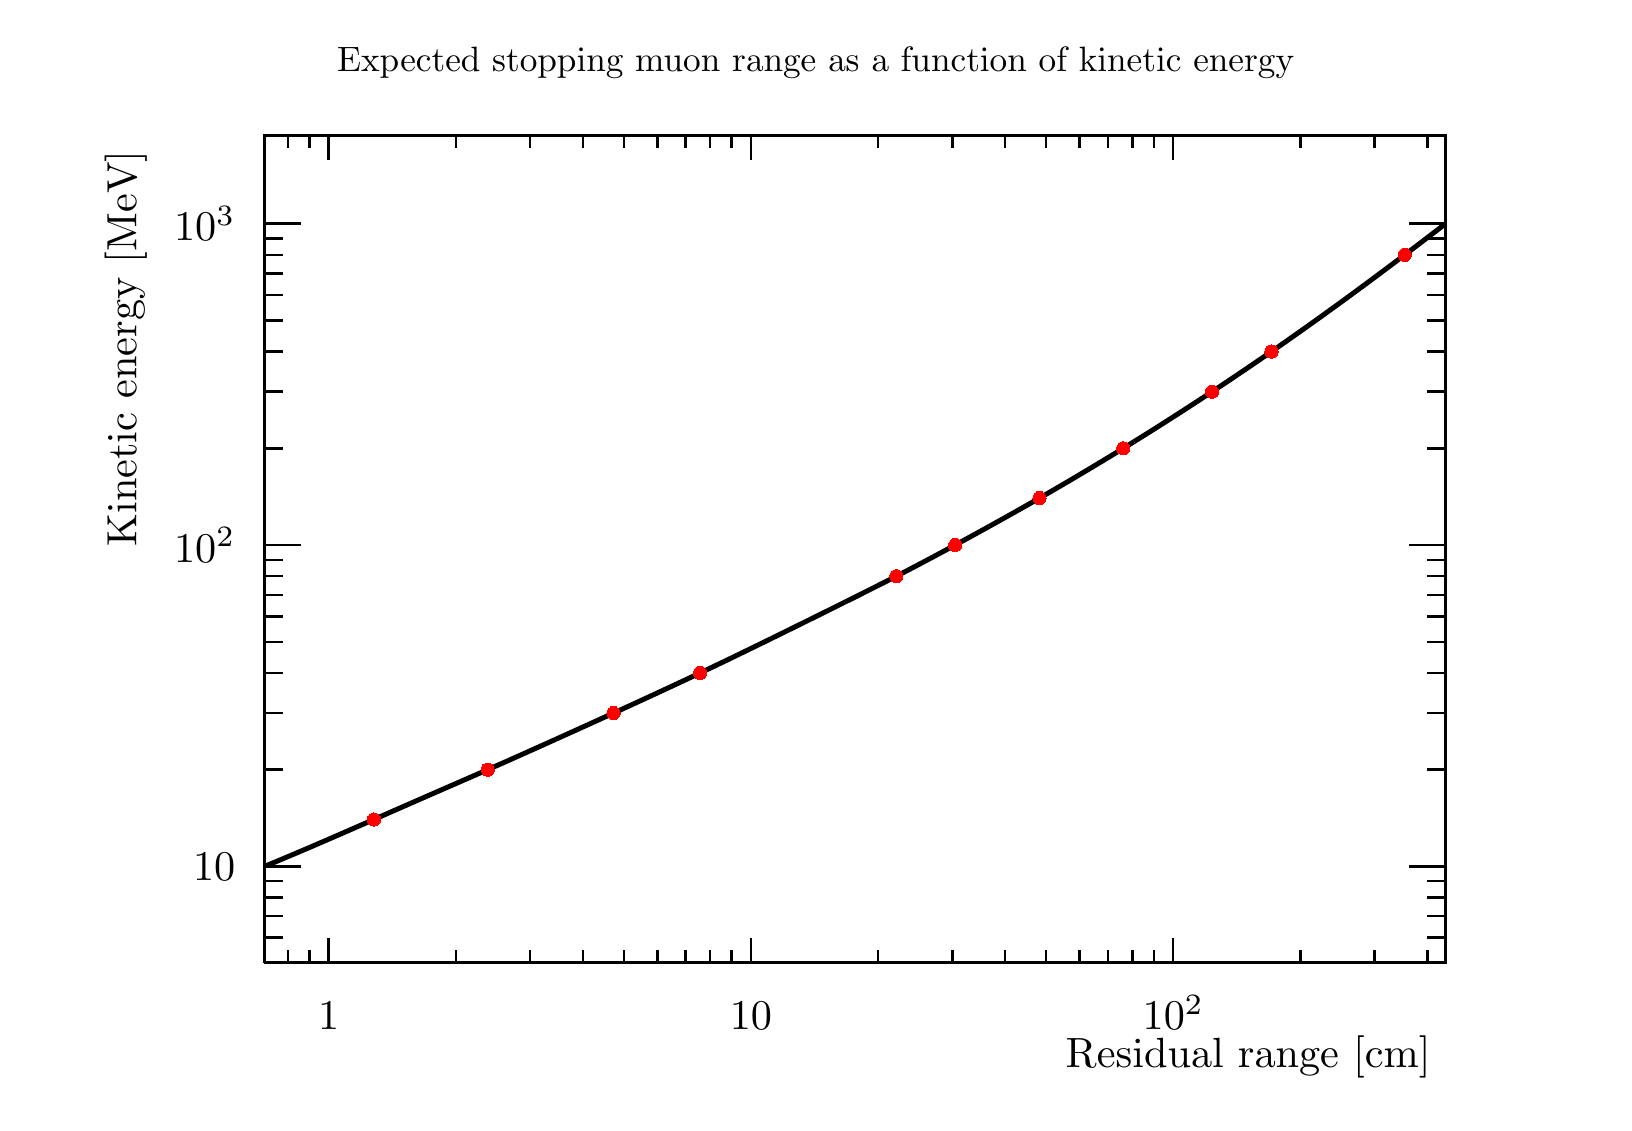
\begin{tikzpicture}
\pgfdeclareplotmark{cross} {
\pgfpathmoveto{\pgfpoint{-0.3\pgfplotmarksize}{\pgfplotmarksize}}
\pgfpathlineto{\pgfpoint{+0.3\pgfplotmarksize}{\pgfplotmarksize}}
\pgfpathlineto{\pgfpoint{+0.3\pgfplotmarksize}{0.3\pgfplotmarksize}}
\pgfpathlineto{\pgfpoint{+1\pgfplotmarksize}{0.3\pgfplotmarksize}}
\pgfpathlineto{\pgfpoint{+1\pgfplotmarksize}{-0.3\pgfplotmarksize}}
\pgfpathlineto{\pgfpoint{+0.3\pgfplotmarksize}{-0.3\pgfplotmarksize}}
\pgfpathlineto{\pgfpoint{+0.3\pgfplotmarksize}{-1.\pgfplotmarksize}}
\pgfpathlineto{\pgfpoint{-0.3\pgfplotmarksize}{-1.\pgfplotmarksize}}
\pgfpathlineto{\pgfpoint{-0.3\pgfplotmarksize}{-0.3\pgfplotmarksize}}
\pgfpathlineto{\pgfpoint{-1.\pgfplotmarksize}{-0.3\pgfplotmarksize}}
\pgfpathlineto{\pgfpoint{-1.\pgfplotmarksize}{0.3\pgfplotmarksize}}
\pgfpathlineto{\pgfpoint{-0.3\pgfplotmarksize}{0.3\pgfplotmarksize}}
\pgfpathclose
\pgfusepathqstroke
}
\pgfdeclareplotmark{cross*} {
\pgfpathmoveto{\pgfpoint{-0.3\pgfplotmarksize}{\pgfplotmarksize}}
\pgfpathlineto{\pgfpoint{+0.3\pgfplotmarksize}{\pgfplotmarksize}}
\pgfpathlineto{\pgfpoint{+0.3\pgfplotmarksize}{0.3\pgfplotmarksize}}
\pgfpathlineto{\pgfpoint{+1\pgfplotmarksize}{0.3\pgfplotmarksize}}
\pgfpathlineto{\pgfpoint{+1\pgfplotmarksize}{-0.3\pgfplotmarksize}}
\pgfpathlineto{\pgfpoint{+0.3\pgfplotmarksize}{-0.3\pgfplotmarksize}}
\pgfpathlineto{\pgfpoint{+0.3\pgfplotmarksize}{-1.\pgfplotmarksize}}
\pgfpathlineto{\pgfpoint{-0.3\pgfplotmarksize}{-1.\pgfplotmarksize}}
\pgfpathlineto{\pgfpoint{-0.3\pgfplotmarksize}{-0.3\pgfplotmarksize}}
\pgfpathlineto{\pgfpoint{-1.\pgfplotmarksize}{-0.3\pgfplotmarksize}}
\pgfpathlineto{\pgfpoint{-1.\pgfplotmarksize}{0.3\pgfplotmarksize}}
\pgfpathlineto{\pgfpoint{-0.3\pgfplotmarksize}{0.3\pgfplotmarksize}}
\pgfpathclose
\pgfusepathqfillstroke
}
\pgfdeclareplotmark{newstar} {
\pgfpathmoveto{\pgfqpoint{0pt}{\pgfplotmarksize}}
\pgfpathlineto{\pgfqpointpolar{44}{0.5\pgfplotmarksize}}
\pgfpathlineto{\pgfqpointpolar{18}{\pgfplotmarksize}}
\pgfpathlineto{\pgfqpointpolar{-20}{0.5\pgfplotmarksize}}
\pgfpathlineto{\pgfqpointpolar{-54}{\pgfplotmarksize}}
\pgfpathlineto{\pgfqpointpolar{-90}{0.5\pgfplotmarksize}}
\pgfpathlineto{\pgfqpointpolar{234}{\pgfplotmarksize}}
\pgfpathlineto{\pgfqpointpolar{198}{0.5\pgfplotmarksize}}
\pgfpathlineto{\pgfqpointpolar{162}{\pgfplotmarksize}}
\pgfpathlineto{\pgfqpointpolar{134}{0.5\pgfplotmarksize}}
\pgfpathclose
\pgfusepathqstroke
}
\pgfdeclareplotmark{newstar*} {
\pgfpathmoveto{\pgfqpoint{0pt}{\pgfplotmarksize}}
\pgfpathlineto{\pgfqpointpolar{44}{0.5\pgfplotmarksize}}
\pgfpathlineto{\pgfqpointpolar{18}{\pgfplotmarksize}}
\pgfpathlineto{\pgfqpointpolar{-20}{0.5\pgfplotmarksize}}
\pgfpathlineto{\pgfqpointpolar{-54}{\pgfplotmarksize}}
\pgfpathlineto{\pgfqpointpolar{-90}{0.5\pgfplotmarksize}}
\pgfpathlineto{\pgfqpointpolar{234}{\pgfplotmarksize}}
\pgfpathlineto{\pgfqpointpolar{198}{0.5\pgfplotmarksize}}
\pgfpathlineto{\pgfqpointpolar{162}{\pgfplotmarksize}}
\pgfpathlineto{\pgfqpointpolar{134}{0.5\pgfplotmarksize}}
\pgfpathclose
\pgfusepathqfillstroke
}
\definecolor{c}{rgb}{1,1,1};
\draw [color=c, fill=c] (0,0) rectangle (20,13.639);
\draw [color=c, fill=c] (3,1.77307) rectangle (18,12.2751);
\definecolor{c}{rgb}{0,0,0};
\draw [c,line width=0.9] (3,1.77307) -- (3,12.2751) -- (18,12.2751) -- (18,1.77307) -- (3,1.77307);
\definecolor{c}{rgb}{1,1,1};
\draw [color=c, fill=c] (0,0) rectangle (20,13.639);
\draw [color=c, fill=c] (3,1.77307) rectangle (18,12.2751);
\definecolor{c}{rgb}{0,0,0};
\draw [c,line width=0.9] (3,1.77307) -- (3,12.2751) -- (18,12.2751) -- (18,1.77307) -- (3,1.77307);
\draw [c,line width=1.8] (3.01883,3.00168) -- (3.05633,3.01716) -- (3.09383,3.03268) -- (3.13133,3.04826) -- (3.16883,3.06388) -- (3.20633,3.07955) -- (3.24383,3.09526) -- (3.28133,3.11102) -- (3.31883,3.12682) -- (3.35633,3.14266) --
 (3.39383,3.15854) -- (3.43133,3.17446) -- (3.46883,3.19042) -- (3.50633,3.20641) -- (3.54383,3.22244) -- (3.58133,3.2385) -- (3.61883,3.25459) -- (3.65633,3.27071) -- (3.69383,3.28686) -- (3.73133,3.30304) -- (3.76883,3.31925) -- (3.80633,3.33548)
 -- (3.84383,3.35173) -- (3.88133,3.36801) -- (3.91883,3.38431) -- (3.95633,3.40063) -- (3.99383,3.41696) -- (4.03133,3.43332) -- (4.06883,3.44968) -- (4.10633,3.46607) -- (4.14383,3.48246) -- (4.18133,3.49887) -- (4.21883,3.51529) --
 (4.25633,3.53172) -- (4.29383,3.54816) -- (4.33133,3.5646) -- (4.36883,3.58105) -- (4.40633,3.59751) -- (4.44383,3.61397) -- (4.48133,3.63043) -- (4.51883,3.64689) -- (4.55633,3.66335) -- (4.59383,3.67982) -- (4.63133,3.69628) -- (4.66883,3.71274)
 -- (4.70633,3.72919) -- (4.74383,3.74565) -- (4.78133,3.7621) -- (4.81883,3.77854) -- (4.85633,3.79498);
\draw [c,line width=1.8] (4.85633,3.79498) -- (4.89383,3.81141) -- (4.93133,3.82784) -- (4.96883,3.84426) -- (5.00633,3.86067) -- (5.04383,3.87707) -- (5.08133,3.89347) -- (5.11883,3.90986) -- (5.15633,3.92625) -- (5.19383,3.94262) -- (5.23133,3.959)
 -- (5.26883,3.97536) -- (5.30633,3.99172) -- (5.34383,4.00808) -- (5.38133,4.02444) -- (5.41883,4.04079) -- (5.45633,4.05714) -- (5.49383,4.0735) -- (5.53133,4.08985) -- (5.56883,4.10621) -- (5.60633,4.12258) -- (5.64383,4.13896) --
 (5.68133,4.15535) -- (5.71883,4.17176) -- (5.75633,4.18818) -- (5.79383,4.20463) -- (5.83133,4.2211) -- (5.86883,4.2376) -- (5.90633,4.25413) -- (5.94383,4.27069) -- (5.98133,4.28727) -- (6.01883,4.30388) -- (6.05633,4.32052) -- (6.09383,4.33717) --
 (6.13133,4.35385) -- (6.16883,4.37055) -- (6.20633,4.38728) -- (6.24383,4.40402) -- (6.28133,4.42077) -- (6.31883,4.43755) -- (6.35633,4.45434) -- (6.39383,4.47115) -- (6.43133,4.48797) -- (6.46883,4.50481) -- (6.50633,4.52165) -- (6.54383,4.53851)
 -- (6.58133,4.55538) -- (6.61883,4.57227) -- (6.65633,4.58916) -- (6.69383,4.60606);
\draw [c,line width=1.8] (6.69383,4.60606) -- (6.73133,4.62297) -- (6.76883,4.63989) -- (6.80633,4.65682) -- (6.84383,4.67375) -- (6.88133,4.6907) -- (6.91883,4.70765) -- (6.95633,4.72461) -- (6.99383,4.74157) -- (7.03133,4.75855) --
 (7.06883,4.77553) -- (7.10633,4.79252) -- (7.14383,4.80952) -- (7.18133,4.82653) -- (7.21883,4.84356) -- (7.25633,4.86059) -- (7.29383,4.87764) -- (7.33133,4.89469) -- (7.36883,4.91177) -- (7.40633,4.92886) -- (7.44383,4.94597) -- (7.48133,4.9631)
 -- (7.51883,4.98025) -- (7.55633,4.99741) -- (7.59383,5.0146) -- (7.63133,5.0318) -- (7.66883,5.04902) -- (7.70633,5.06626) -- (7.74383,5.08351) -- (7.78133,5.10078) -- (7.81883,5.11806) -- (7.85633,5.13537) -- (7.89383,5.15268) -- (7.93133,5.17002)
 -- (7.96883,5.18737) -- (8.00633,5.20474) -- (8.04383,5.22213) -- (8.08133,5.23954) -- (8.11883,5.25696) -- (8.15633,5.27441) -- (8.19383,5.29188) -- (8.23133,5.30936) -- (8.26883,5.32688) -- (8.30633,5.34442) -- (8.34383,5.36198) --
 (8.38133,5.37957) -- (8.41883,5.3972) -- (8.45633,5.41485) -- (8.49383,5.43254) -- (8.53133,5.45027);
\draw [c,line width=1.8] (8.53133,5.45027) -- (8.56883,5.46804) -- (8.60633,5.48585) -- (8.64383,5.50369) -- (8.68133,5.52157) -- (8.71883,5.53949) -- (8.75633,5.55744) -- (8.79383,5.57543) -- (8.83133,5.59345) -- (8.86883,5.6115) --
 (8.90633,5.62958) -- (8.94383,5.64769) -- (8.98133,5.66582) -- (9.01883,5.68399) -- (9.05633,5.70218) -- (9.09383,5.72039) -- (9.13133,5.73863) -- (9.16883,5.75689) -- (9.20633,5.77517) -- (9.24383,5.79348) -- (9.28133,5.8118) -- (9.31883,5.83014)
 -- (9.35633,5.8485) -- (9.39383,5.86688) -- (9.43133,5.88527) -- (9.46883,5.90368) -- (9.50633,5.9221) -- (9.54383,5.94054) -- (9.58133,5.95899) -- (9.61883,5.97745) -- (9.65633,5.99593) -- (9.69383,6.01441) -- (9.73133,6.03291) -- (9.76883,6.05142)
 -- (9.80633,6.06994) -- (9.84383,6.08846) -- (9.88133,6.107) -- (9.91883,6.12555) -- (9.95633,6.1441) -- (9.99383,6.16267) -- (10.0313,6.18124) -- (10.0688,6.19983) -- (10.1063,6.21842) -- (10.1438,6.23702) -- (10.1813,6.25564) -- (10.2188,6.27426)
 -- (10.2563,6.2929) -- (10.2938,6.31154) -- (10.3313,6.3302) -- (10.3688,6.34888);
\draw [c,line width=1.8] (10.3688,6.34888) -- (10.4063,6.36757) -- (10.4438,6.38628) -- (10.4813,6.405) -- (10.5188,6.42374) -- (10.5563,6.44251) -- (10.5938,6.4613) -- (10.6313,6.48011) -- (10.6688,6.49895) -- (10.7063,6.51782) -- (10.7438,6.53673)
 -- (10.7813,6.55567) -- (10.8188,6.57464) -- (10.8563,6.59366) -- (10.8938,6.61273) -- (10.9313,6.63185) -- (10.9688,6.65102) -- (11.0063,6.67025) -- (11.0438,6.68954) -- (11.0813,6.7089) -- (11.1188,6.72832) -- (11.1563,6.7478) -- (11.1938,6.76735)
 -- (11.2313,6.78695) -- (11.2688,6.80662) -- (11.3063,6.82634) -- (11.3438,6.84611) -- (11.3813,6.86594) -- (11.4188,6.88583) -- (11.4563,6.90577) -- (11.4938,6.92575) -- (11.5313,6.94579) -- (11.5688,6.96587) -- (11.6063,6.986) -- (11.6438,7.00617)
 -- (11.6813,7.02639) -- (11.7188,7.04665) -- (11.7563,7.06694) -- (11.7938,7.08728) -- (11.8313,7.10765) -- (11.8688,7.12806) -- (11.9063,7.14851) -- (11.9438,7.16899) -- (11.9813,7.18951) -- (12.0188,7.21006) -- (12.0563,7.23065) --
 (12.0938,7.25128) -- (12.1313,7.27194) -- (12.1688,7.29264) -- (12.2063,7.31338);
\draw [c,line width=1.8] (12.2063,7.31338) -- (12.2438,7.33416) -- (12.2813,7.35497) -- (12.3188,7.37582) -- (12.3563,7.39671) -- (12.3938,7.41764) -- (12.4313,7.4386) -- (12.4688,7.45961) -- (12.5063,7.48066) -- (12.5438,7.50176) --
 (12.5813,7.52289) -- (12.6188,7.54408) -- (12.6563,7.5653) -- (12.6938,7.58658) -- (12.7313,7.60791) -- (12.7688,7.62928) -- (12.8063,7.65071) -- (12.8438,7.67219) -- (12.8813,7.69374) -- (12.9188,7.71533) -- (12.9563,7.73698) -- (12.9938,7.75869)
 -- (13.0313,7.78046) -- (13.0688,7.80227) -- (13.1063,7.82415) -- (13.1438,7.84607) -- (13.1813,7.86806) -- (13.2188,7.89009) -- (13.2563,7.91218) -- (13.2938,7.93432) -- (13.3313,7.95652) -- (13.3688,7.97877) -- (13.4063,8.00107) --
 (13.4438,8.02342) -- (13.4813,8.04583) -- (13.5188,8.06829) -- (13.5563,8.09081) -- (13.5938,8.11338) -- (13.6313,8.136) -- (13.6688,8.15868) -- (13.7063,8.18141) -- (13.7438,8.20419) -- (13.7813,8.22704) -- (13.8188,8.24993) -- (13.8563,8.27289) --
 (13.8938,8.2959) -- (13.9313,8.31897) -- (13.9688,8.3421) -- (14.0063,8.36528) -- (14.0438,8.38852);
\draw [c,line width=1.8] (14.0438,8.38852) -- (14.0813,8.41182) -- (14.1188,8.43518) -- (14.1563,8.45859) -- (14.1938,8.48206) -- (14.2313,8.50558) -- (14.2688,8.52916) -- (14.3063,8.55279) -- (14.3438,8.57648) -- (14.3813,8.60023) --
 (14.4188,8.62403) -- (14.4563,8.64788) -- (14.4938,8.67179) -- (14.5313,8.69575) -- (14.5688,8.71977) -- (14.6063,8.74385) -- (14.6438,8.76797) -- (14.6813,8.79216) -- (14.7188,8.8164) -- (14.7563,8.84069) -- (14.7938,8.86504) -- (14.8313,8.88945)
 -- (14.8688,8.91391) -- (14.9063,8.93843) -- (14.9438,8.96301) -- (14.9813,8.98765) -- (15.0188,9.01234) -- (15.0563,9.03709) -- (15.0938,9.0619) -- (15.1313,9.08677) -- (15.1688,9.1117) -- (15.2063,9.13669) -- (15.2438,9.16174) -- (15.2813,9.18684)
 -- (15.3188,9.21201) -- (15.3563,9.23723) -- (15.3938,9.26252) -- (15.4313,9.28786) -- (15.4688,9.31326) -- (15.5063,9.33872) -- (15.5438,9.36424) -- (15.5813,9.38982) -- (15.6188,9.41546) -- (15.6563,9.44116) -- (15.6938,9.46692) --
 (15.7313,9.49275) -- (15.7688,9.51863) -- (15.8063,9.54458) -- (15.8438,9.57059) -- (15.8813,9.59666);
\draw [c,line width=1.8] (15.8813,9.59666) -- (15.9188,9.62279) -- (15.9563,9.64898) -- (15.9938,9.67524) -- (16.0313,9.70155) -- (16.0688,9.72792) -- (16.1063,9.75436) -- (16.1438,9.78085) -- (16.1813,9.8074) -- (16.2188,9.834) -- (16.2563,9.86067)
 -- (16.2938,9.88739) -- (16.3313,9.91416) -- (16.3688,9.941) -- (16.4063,9.96789) -- (16.4438,9.99483) -- (16.4813,10.0218) -- (16.5188,10.0489) -- (16.5563,10.076) -- (16.5938,10.1031) -- (16.6313,10.1304) -- (16.6688,10.1576) -- (16.7063,10.1849)
 -- (16.7438,10.2123) -- (16.7813,10.2397) -- (16.8188,10.2672) -- (16.8563,10.2947) -- (16.8938,10.3223) -- (16.9313,10.3499) -- (16.9688,10.3776) -- (17.0063,10.4053) -- (17.0438,10.4331) -- (17.0813,10.4609) -- (17.1188,10.4888) --
 (17.1563,10.5167) -- (17.1938,10.5447) -- (17.2313,10.5727) -- (17.2688,10.6008) -- (17.3063,10.6289) -- (17.3438,10.657) -- (17.3813,10.6852) -- (17.4188,10.7135) -- (17.4563,10.7418) -- (17.4938,10.7701) -- (17.5313,10.7985) -- (17.5688,10.8269)
 -- (17.6063,10.8554) -- (17.6438,10.8839) -- (17.6813,10.9124) -- (17.7188,10.941);
\draw [c,line width=1.8] (17.7188,10.941) -- (17.7563,10.9696) -- (17.7938,10.9983) -- (17.8313,11.027) -- (17.8688,11.0558) -- (17.9063,11.0846) -- (17.9438,11.1134) -- (17.9813,11.1423);
\draw [c,line width=0.9] (3,1.77307) -- (18,1.77307);
\draw [c,line width=0.9] (3.2965,1.9265) -- (3.2965,1.77307);
\draw [c,line width=0.9] (3.57082,1.9265) -- (3.57082,1.77307);
\draw [c,line width=0.9] (3.8162,2.07994) -- (3.8162,1.77307);
\draw [anchor=base] (3.8162,0.92063) node[scale=1.52731, color=c, rotate=0]{1};
\draw [c,line width=0.9] (5.43053,1.9265) -- (5.43053,1.77307);
\draw [c,line width=0.9] (6.37485,1.9265) -- (6.37485,1.77307);
\draw [c,line width=0.9] (7.04486,1.9265) -- (7.04486,1.77307);
\draw [c,line width=0.9] (7.56456,1.9265) -- (7.56456,1.77307);
\draw [c,line width=0.9] (7.98918,1.9265) -- (7.98918,1.77307);
\draw [c,line width=0.9] (8.34819,1.9265) -- (8.34819,1.77307);
\draw [c,line width=0.9] (8.65919,1.9265) -- (8.65919,1.77307);
\draw [c,line width=0.9] (8.9335,1.9265) -- (8.9335,1.77307);
\draw [c,line width=0.9] (9.17888,2.07994) -- (9.17888,1.77307);
\draw [anchor=base] (9.17888,0.92063) node[scale=1.52731, color=c, rotate=0]{10};
\draw [c,line width=0.9] (10.7932,1.9265) -- (10.7932,1.77307);
\draw [c,line width=0.9] (11.7375,1.9265) -- (11.7375,1.77307);
\draw [c,line width=0.9] (12.4075,1.9265) -- (12.4075,1.77307);
\draw [c,line width=0.9] (12.9272,1.9265) -- (12.9272,1.77307);
\draw [c,line width=0.9] (13.3519,1.9265) -- (13.3519,1.77307);
\draw [c,line width=0.9] (13.7109,1.9265) -- (13.7109,1.77307);
\draw [c,line width=0.9] (14.0219,1.9265) -- (14.0219,1.77307);
\draw [c,line width=0.9] (14.2962,1.9265) -- (14.2962,1.77307);
\draw [c,line width=0.9] (14.5416,2.07994) -- (14.5416,1.77307);
\draw [anchor=base] (14.5416,0.92063) node[scale=1.52731, color=c, rotate=0]{$10^{2}$};
\draw [c,line width=0.9] (16.1559,1.9265) -- (16.1559,1.77307);
\draw [c,line width=0.9] (17.1002,1.9265) -- (17.1002,1.77307);
\draw [c,line width=0.9] (17.7702,1.9265) -- (17.7702,1.77307);
\draw [anchor= east] (18,0.572837) node[scale=1.52731, color=c, rotate=0]{ Residual range [cm]};
\draw [c,line width=0.9] (3,12.2751) -- (18,12.2751);
\draw [c,line width=0.9] (3.2965,12.1216) -- (3.2965,12.2751);
\draw [c,line width=0.9] (3.57082,12.1216) -- (3.57082,12.2751);
\draw [c,line width=0.9] (3.8162,11.9682) -- (3.8162,12.2751);
\draw [c,line width=0.9] (5.43053,12.1216) -- (5.43053,12.2751);
\draw [c,line width=0.9] (6.37485,12.1216) -- (6.37485,12.2751);
\draw [c,line width=0.9] (7.04486,12.1216) -- (7.04486,12.2751);
\draw [c,line width=0.9] (7.56456,12.1216) -- (7.56456,12.2751);
\draw [c,line width=0.9] (7.98918,12.1216) -- (7.98918,12.2751);
\draw [c,line width=0.9] (8.34819,12.1216) -- (8.34819,12.2751);
\draw [c,line width=0.9] (8.65919,12.1216) -- (8.65919,12.2751);
\draw [c,line width=0.9] (8.9335,12.1216) -- (8.9335,12.2751);
\draw [c,line width=0.9] (9.17888,11.9682) -- (9.17888,12.2751);
\draw [c,line width=0.9] (10.7932,12.1216) -- (10.7932,12.2751);
\draw [c,line width=0.9] (11.7375,12.1216) -- (11.7375,12.2751);
\draw [c,line width=0.9] (12.4075,12.1216) -- (12.4075,12.2751);
\draw [c,line width=0.9] (12.9272,12.1216) -- (12.9272,12.2751);
\draw [c,line width=0.9] (13.3519,12.1216) -- (13.3519,12.2751);
\draw [c,line width=0.9] (13.7109,12.1216) -- (13.7109,12.2751);
\draw [c,line width=0.9] (14.0219,12.1216) -- (14.0219,12.2751);
\draw [c,line width=0.9] (14.2962,12.1216) -- (14.2962,12.2751);
\draw [c,line width=0.9] (14.5416,11.9682) -- (14.5416,12.2751);
\draw [c,line width=0.9] (16.1559,12.1216) -- (16.1559,12.2751);
\draw [c,line width=0.9] (17.1002,12.1216) -- (17.1002,12.2751);
\draw [c,line width=0.9] (17.7702,12.1216) -- (17.7702,12.2751);
\draw [c,line width=0.9] (3,1.77307) -- (3,12.2751);
\draw [c,line width=0.9] (3.231,2.08848) -- (3,2.08848);
\draw [c,line width=0.9] (3.231,2.36172) -- (3,2.36172);
\draw [c,line width=0.9] (3.231,2.5984) -- (3,2.5984);
\draw [c,line width=0.9] (3.231,2.80718) -- (3,2.80718);
\draw [c,line width=0.9] (3.462,2.99393) -- (3,2.99393);
\draw [anchor= east] (2.82,2.99393) node[scale=1.52731, color=c, rotate=0]{10};
\draw [c,line width=0.9] (3.231,4.22255) -- (3,4.22255);
\draw [c,line width=0.9] (3.231,4.94124) -- (3,4.94124);
\draw [c,line width=0.9] (3.231,5.45116) -- (3,5.45116);
\draw [c,line width=0.9] (3.231,5.84669) -- (3,5.84669);
\draw [c,line width=0.9] (3.231,6.16986) -- (3,6.16986);
\draw [c,line width=0.9] (3.231,6.44309) -- (3,6.44309);
\draw [c,line width=0.9] (3.231,6.67978) -- (3,6.67978);
\draw [c,line width=0.9] (3.231,6.88855) -- (3,6.88855);
\draw [c,line width=0.9] (3.462,7.07531) -- (3,7.07531);
\draw [anchor= east] (2.82,7.07531) node[scale=1.52731, color=c, rotate=0]{$10^{2}$};
\draw [c,line width=0.9] (3.231,8.30392) -- (3,8.30392);
\draw [c,line width=0.9] (3.231,9.02262) -- (3,9.02262);
\draw [c,line width=0.9] (3.231,9.53254) -- (3,9.53254);
\draw [c,line width=0.9] (3.231,9.92807) -- (3,9.92807);
\draw [c,line width=0.9] (3.231,10.2512) -- (3,10.2512);
\draw [c,line width=0.9] (3.231,10.5245) -- (3,10.5245);
\draw [c,line width=0.9] (3.231,10.7612) -- (3,10.7612);
\draw [c,line width=0.9] (3.231,10.9699) -- (3,10.9699);
\draw [c,line width=0.9] (3.462,11.1567) -- (3,11.1567);
\draw [anchor= east] (2.82,11.1567) node[scale=1.52731, color=c, rotate=0]{$10^{3}$};
\draw [anchor= east] (1.24,12.2751) node[scale=1.52731, color=c, rotate=90]{ Kinetic energy [MeV]};
\draw [c,line width=0.9] (18,1.77307) -- (18,12.2751);
\draw [c,line width=0.9] (17.769,2.08848) -- (18,2.08848);
\draw [c,line width=0.9] (17.769,2.36172) -- (18,2.36172);
\draw [c,line width=0.9] (17.769,2.5984) -- (18,2.5984);
\draw [c,line width=0.9] (17.769,2.80718) -- (18,2.80718);
\draw [c,line width=0.9] (17.538,2.99393) -- (18,2.99393);
\draw [c,line width=0.9] (17.769,4.22255) -- (18,4.22255);
\draw [c,line width=0.9] (17.769,4.94124) -- (18,4.94124);
\draw [c,line width=0.9] (17.769,5.45116) -- (18,5.45116);
\draw [c,line width=0.9] (17.769,5.84669) -- (18,5.84669);
\draw [c,line width=0.9] (17.769,6.16986) -- (18,6.16986);
\draw [c,line width=0.9] (17.769,6.44309) -- (18,6.44309);
\draw [c,line width=0.9] (17.769,6.67978) -- (18,6.67978);
\draw [c,line width=0.9] (17.769,6.88855) -- (18,6.88855);
\draw [c,line width=0.9] (17.538,7.07531) -- (18,7.07531);
\draw [c,line width=0.9] (17.769,8.30392) -- (18,8.30392);
\draw [c,line width=0.9] (17.769,9.02262) -- (18,9.02262);
\draw [c,line width=0.9] (17.769,9.53254) -- (18,9.53254);
\draw [c,line width=0.9] (17.769,9.92807) -- (18,9.92807);
\draw [c,line width=0.9] (17.769,10.2512) -- (18,10.2512);
\draw [c,line width=0.9] (17.769,10.5245) -- (18,10.5245);
\draw [c,line width=0.9] (17.769,10.7612) -- (18,10.7612);
\draw [c,line width=0.9] (17.769,10.9699) -- (18,10.9699);
\draw [c,line width=0.9] (17.538,11.1567) -- (18,11.1567);
\definecolor{c}{rgb}{1,0,0};
\foreach \P in {(4.38998,3.59034), (5.83462,4.22255), (7.43347,4.94124), (8.53322,5.45117), (11.0249,6.67978), (11.7718,7.07531), (12.843,7.67171), (13.9069,8.30392), (15.0344,9.02262), (15.7889,9.53254), (17.482,10.7612)}{\draw[mark
 options={color=c,fill=c},mark size=2.402402pt, line width=0.000000pt, mark=*] plot coordinates {\P};}
\definecolor{c}{rgb}{1,1,1};
\draw [color=c, fill=c] (2,12.8206) rectangle (18,13.5708);
\definecolor{c}{rgb}{0,0,0};
\draw (10,13.1957) node[scale=1.27276, color=c, rotate=0]{Expected stopping muon range as a function of kinetic energy};
\end{tikzpicture}

	\end{adjustbox}
	\caption[Muon range in liquid argon as a function of kinetic energy]{Muon range in liquid argon under the continuous slowing down approximation (CSDA) as a function of kinetic energy. The red points are taken from~\cite{muonCSDA}. The black line is a cubic spline drawn through the points.}
	\label{fig:keVsRange}
\end{figure}

%% Track selection
From \citefig{fig:muonEDep} left and right, one can see that, aside from the last 40 or \SI{50}{\cm} of the track, muons will have uniform energy deposition in liquid argon.
Therefore, any track selection used for detector calibration should avoid using the ends of muon tracks.
However, excluding the last \SI{50}{\cm} of all muon tracks regardless of if they stop in the detector or not would result in a significant volume of the detector which could not be effectively calibrated by this method.
Therefore, it is decided to instead select all those cosmic ray tracks which exit the detector and assume that they are not close to stopping.
Specifically, those tracks that cross the cathode and at least one of the anodes are selected.

Requiring that tracks cross the cathode and an anode has two outcomes.
Firstly, it ensures that all the selected tracks have lengths equal to at least the drift distance and excludes short tracks that may be more easily mis-reconstructed.

Secondly, it allows the tracks to be given a definite time at which they entered the TPC.
As mentioned in \citesec{sec:dune:fd:lartpc}, TPCs such as ProtoDUNE-SP produce multiple 2-dimensional images which can be combined via reconstruction algorithms~\cite{pandora} to form 3-dimensional reconstructed tracks.
Typically, for neutrino induced events in LAr TPCs a definite drift coordinate can be reconstructed using timing information from the neutrino beam.

However for external particles such as cosmic rays, which are impinging on the detector continuously, this beam timing information is obviously not available.
Instead, reconstruction techniques must be utilised.

Specifically, the Pandora software package~\cite{pandora} looks at tracks in the two TPCs, separated by the central cathode.
If two 3-dimensional clusters in neighbouring drift volumes have similar direction vectors and an equal and opposite shift in the drift direction from the cathode, they can be stitched across the cathode to form one larger track.
This track will therefore have a definite time at which it crossed the cathode, often termed a $t_{0}$.
In turn, this allows definite drift coordinates and times to be reconstructed for all points in the track via the equation
\begin{equation}
	t_{\text{drift}} = t_{\text{hit}} - t_{0} \, ,
\end{equation}
where $t_{\text{hit}}$ is the recorded hit time in the TPC.

Cosmic rays are identified by the Pandora reconstruction chain. 
This reconstruction chain focusses on reconstructing track-like particle and has been shown to work well in the MicroBooNE experiment~\cite{pandoraUboone}. 
Tracks satisfying one of three conditions are considered to be produced by cosmic rays.
Firstly, those tracks starting at the top of the detector and ending at the bottom are considered to be cosmic rays.
Secondly, those tracks with a reconstructed $t_{0}$ which is inconsistent with the beam time are also considered to be cosmic rays.
Finally, any tracks which have reconstructed hits which appear to be outside the detector when assuming $t_0 = 0$ are considered to be inconsistent with beam particles and are thus cosmic rays.

%% Angular cuts explanation
Constraints are also placed on the angle of tracks used in the selection.
These constraints are in place due to difficulties in reconstructing the track \dqdx at certain angles.
This issue is shown in \citefig{fig:dqdxAng} which shows the average track \dqdx as a function of two angles, \thetai{yx} and \thetai{yz}.
One can see that at certain values of \thetai{xz} (around $\pm\ang{90}$) and \thetai{yz} (around \ang{-90}) the average track \dqdx falls significantly.
The difference around $\thetai{xz} = \pm \ang{90}$ is caused by tracks travelling close to parallel with the drift direction while the difference at $\thetai{yz} = \ang{-90}$ is due to tracks travelling vertically downwards.

\begin{figure}[h]
	\begin{adjustbox}{max totalsize=.6\textwidth, center}
		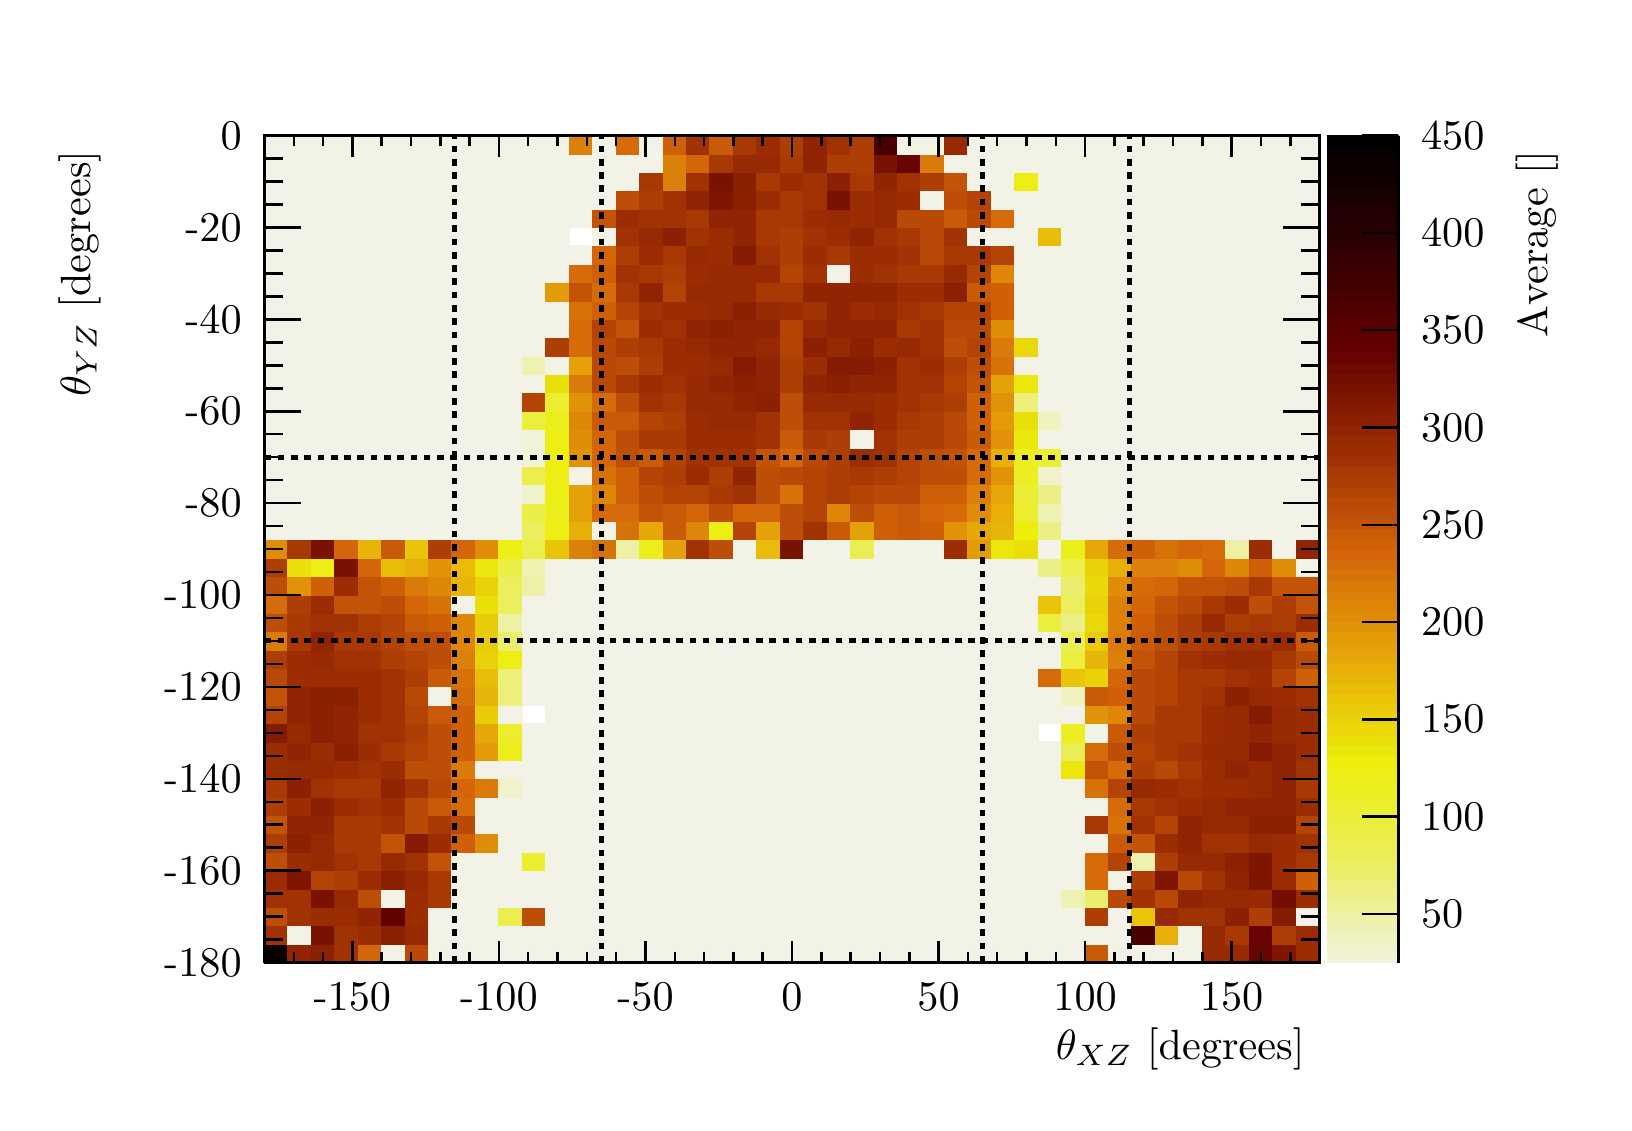
\begin{tikzpicture}
\pgfdeclareplotmark{cross} {
\pgfpathmoveto{\pgfpoint{-0.3\pgfplotmarksize}{\pgfplotmarksize}}
\pgfpathlineto{\pgfpoint{+0.3\pgfplotmarksize}{\pgfplotmarksize}}
\pgfpathlineto{\pgfpoint{+0.3\pgfplotmarksize}{0.3\pgfplotmarksize}}
\pgfpathlineto{\pgfpoint{+1\pgfplotmarksize}{0.3\pgfplotmarksize}}
\pgfpathlineto{\pgfpoint{+1\pgfplotmarksize}{-0.3\pgfplotmarksize}}
\pgfpathlineto{\pgfpoint{+0.3\pgfplotmarksize}{-0.3\pgfplotmarksize}}
\pgfpathlineto{\pgfpoint{+0.3\pgfplotmarksize}{-1.\pgfplotmarksize}}
\pgfpathlineto{\pgfpoint{-0.3\pgfplotmarksize}{-1.\pgfplotmarksize}}
\pgfpathlineto{\pgfpoint{-0.3\pgfplotmarksize}{-0.3\pgfplotmarksize}}
\pgfpathlineto{\pgfpoint{-1.\pgfplotmarksize}{-0.3\pgfplotmarksize}}
\pgfpathlineto{\pgfpoint{-1.\pgfplotmarksize}{0.3\pgfplotmarksize}}
\pgfpathlineto{\pgfpoint{-0.3\pgfplotmarksize}{0.3\pgfplotmarksize}}
\pgfpathclose
\pgfusepathqstroke
}
\pgfdeclareplotmark{cross*} {
\pgfpathmoveto{\pgfpoint{-0.3\pgfplotmarksize}{\pgfplotmarksize}}
\pgfpathlineto{\pgfpoint{+0.3\pgfplotmarksize}{\pgfplotmarksize}}
\pgfpathlineto{\pgfpoint{+0.3\pgfplotmarksize}{0.3\pgfplotmarksize}}
\pgfpathlineto{\pgfpoint{+1\pgfplotmarksize}{0.3\pgfplotmarksize}}
\pgfpathlineto{\pgfpoint{+1\pgfplotmarksize}{-0.3\pgfplotmarksize}}
\pgfpathlineto{\pgfpoint{+0.3\pgfplotmarksize}{-0.3\pgfplotmarksize}}
\pgfpathlineto{\pgfpoint{+0.3\pgfplotmarksize}{-1.\pgfplotmarksize}}
\pgfpathlineto{\pgfpoint{-0.3\pgfplotmarksize}{-1.\pgfplotmarksize}}
\pgfpathlineto{\pgfpoint{-0.3\pgfplotmarksize}{-0.3\pgfplotmarksize}}
\pgfpathlineto{\pgfpoint{-1.\pgfplotmarksize}{-0.3\pgfplotmarksize}}
\pgfpathlineto{\pgfpoint{-1.\pgfplotmarksize}{0.3\pgfplotmarksize}}
\pgfpathlineto{\pgfpoint{-0.3\pgfplotmarksize}{0.3\pgfplotmarksize}}
\pgfpathclose
\pgfusepathqfillstroke
}
\pgfdeclareplotmark{newstar} {
\pgfpathmoveto{\pgfqpoint{0pt}{\pgfplotmarksize}}
\pgfpathlineto{\pgfqpointpolar{44}{0.5\pgfplotmarksize}}
\pgfpathlineto{\pgfqpointpolar{18}{\pgfplotmarksize}}
\pgfpathlineto{\pgfqpointpolar{-20}{0.5\pgfplotmarksize}}
\pgfpathlineto{\pgfqpointpolar{-54}{\pgfplotmarksize}}
\pgfpathlineto{\pgfqpointpolar{-90}{0.5\pgfplotmarksize}}
\pgfpathlineto{\pgfqpointpolar{234}{\pgfplotmarksize}}
\pgfpathlineto{\pgfqpointpolar{198}{0.5\pgfplotmarksize}}
\pgfpathlineto{\pgfqpointpolar{162}{\pgfplotmarksize}}
\pgfpathlineto{\pgfqpointpolar{134}{0.5\pgfplotmarksize}}
\pgfpathclose
\pgfusepathqstroke
}
\pgfdeclareplotmark{newstar*} {
\pgfpathmoveto{\pgfqpoint{0pt}{\pgfplotmarksize}}
\pgfpathlineto{\pgfqpointpolar{44}{0.5\pgfplotmarksize}}
\pgfpathlineto{\pgfqpointpolar{18}{\pgfplotmarksize}}
\pgfpathlineto{\pgfqpointpolar{-20}{0.5\pgfplotmarksize}}
\pgfpathlineto{\pgfqpointpolar{-54}{\pgfplotmarksize}}
\pgfpathlineto{\pgfqpointpolar{-90}{0.5\pgfplotmarksize}}
\pgfpathlineto{\pgfqpointpolar{234}{\pgfplotmarksize}}
\pgfpathlineto{\pgfqpointpolar{198}{0.5\pgfplotmarksize}}
\pgfpathlineto{\pgfqpointpolar{162}{\pgfplotmarksize}}
\pgfpathlineto{\pgfqpointpolar{134}{0.5\pgfplotmarksize}}
\pgfpathclose
\pgfusepathqfillstroke
}
\definecolor{c}{rgb}{1,1,1};
\draw [color=c, fill=c] (0,0) rectangle (20,13.639);
\draw [color=c, fill=c] (3,1.77307) rectangle (16.4,12.2751);
\definecolor{c}{rgb}{0,0,0};
\draw [c,line width=0.9] (3,1.77307) -- (3,12.2751) -- (16.4,12.2751) -- (16.4,1.77307) -- (3,1.77307);
\definecolor{c}{rgb}{1,1,1};
\draw [color=c, fill=c] (3,1.77307) rectangle (16.4,12.2751);
\definecolor{c}{rgb}{0,0,0};
\draw [c,line width=0.9] (3,1.77307) -- (3,12.2751) -- (16.4,12.2751) -- (16.4,1.77307) -- (3,1.77307);
\definecolor{c}{rgb}{0.0386029,0,0.000857843};
\draw [color=c, fill=c] (3,1.77307) rectangle (3.29778,2.00644);
\definecolor{c}{rgb}{0.569853,0.143382,0.0102941};
\draw [color=c, fill=c] (3.29778,1.77307) rectangle (3.59556,2.00644);
\definecolor{c}{rgb}{0.548897,0.126838,0.00955882};
\draw [color=c, fill=c] (3.59556,1.77307) rectangle (3.89333,2.00644);
\definecolor{c}{rgb}{0.632353,0.197059,0.0139706};
\draw [color=c, fill=c] (3.89333,1.77307) rectangle (4.19111,2.00644);
\definecolor{c}{rgb}{0.831373,0.396078,0.0352941};
\draw [color=c, fill=c] (4.19111,1.77307) rectangle (4.48889,2.00644);
\definecolor{c}{rgb}{0.94902,0.952941,0.901961};
\draw [color=c, fill=c] (4.48889,1.77307) rectangle (4.78667,2.00644);
\definecolor{c}{rgb}{0.721569,0.286275,0.0235294};
\draw [color=c, fill=c] (4.78667,1.77307) rectangle (5.08444,2.00644);
\definecolor{c}{rgb}{0.94902,0.952941,0.901961};
\draw [color=c, fill=c] (5.08444,1.77307) rectangle (5.38222,2.00644);
\draw [color=c, fill=c] (5.38222,1.77307) rectangle (5.68,2.00644);
\draw [color=c, fill=c] (5.68,1.77307) rectangle (5.97778,2.00644);
\draw [color=c, fill=c] (5.97778,1.77307) rectangle (6.27556,2.00644);
\draw [color=c, fill=c] (6.27556,1.77307) rectangle (6.57333,2.00644);
\draw [color=c, fill=c] (6.57333,1.77307) rectangle (6.87111,2.00644);
\draw [color=c, fill=c] (6.87111,1.77307) rectangle (7.16889,2.00644);
\draw [color=c, fill=c] (7.16889,1.77307) rectangle (7.46667,2.00644);
\draw [color=c, fill=c] (7.46667,1.77307) rectangle (7.76444,2.00644);
\draw [color=c, fill=c] (7.76444,1.77307) rectangle (8.06222,2.00644);
\draw [color=c, fill=c] (8.06222,1.77307) rectangle (8.36,2.00644);
\draw [color=c, fill=c] (8.36,1.77307) rectangle (8.65778,2.00644);
\draw [color=c, fill=c] (8.65778,1.77307) rectangle (8.95556,2.00644);
\draw [color=c, fill=c] (8.95556,1.77307) rectangle (9.25333,2.00644);
\draw [color=c, fill=c] (9.25333,1.77307) rectangle (9.55111,2.00644);
\draw [color=c, fill=c] (9.55111,1.77307) rectangle (9.84889,2.00644);
\draw [color=c, fill=c] (9.84889,1.77307) rectangle (10.1467,2.00644);
\draw [color=c, fill=c] (10.1467,1.77307) rectangle (10.4444,2.00644);
\draw [color=c, fill=c] (10.4444,1.77307) rectangle (10.7422,2.00644);
\draw [color=c, fill=c] (10.7422,1.77307) rectangle (11.04,2.00644);
\draw [color=c, fill=c] (11.04,1.77307) rectangle (11.3378,2.00644);
\draw [color=c, fill=c] (11.3378,1.77307) rectangle (11.6356,2.00644);
\draw [color=c, fill=c] (11.6356,1.77307) rectangle (11.9333,2.00644);
\draw [color=c, fill=c] (11.9333,1.77307) rectangle (12.2311,2.00644);
\draw [color=c, fill=c] (12.2311,1.77307) rectangle (12.5289,2.00644);
\draw [color=c, fill=c] (12.5289,1.77307) rectangle (12.8267,2.00644);
\draw [color=c, fill=c] (12.8267,1.77307) rectangle (13.1244,2.00644);
\draw [color=c, fill=c] (13.1244,1.77307) rectangle (13.4222,2.00644);
\definecolor{c}{rgb}{0.790196,0.354902,0.0308824};
\draw [color=c, fill=c] (13.4222,1.77307) rectangle (13.72,2.00644);
\definecolor{c}{rgb}{0.94902,0.952941,0.901961};
\draw [color=c, fill=c] (13.72,1.77307) rectangle (14.0178,2.00644);
\draw [color=c, fill=c] (14.0178,1.77307) rectangle (14.3156,2.00644);
\draw [color=c, fill=c] (14.3156,1.77307) rectangle (14.6133,2.00644);
\draw [color=c, fill=c] (14.6133,1.77307) rectangle (14.9111,2.00644);
\definecolor{c}{rgb}{0.590809,0.159926,0.0110294};
\draw [color=c, fill=c] (14.9111,1.77307) rectangle (15.2089,2.00644);
\draw [color=c, fill=c] (15.2089,1.77307) rectangle (15.5067,2.00644);
\definecolor{c}{rgb}{0.409191,0.0165441,0.00465686};
\draw [color=c, fill=c] (15.5067,1.77307) rectangle (15.8044,2.00644);
\definecolor{c}{rgb}{0.5,0.0882353,0.00784314};
\draw [color=c, fill=c] (15.8044,1.77307) rectangle (16.1022,2.00644);
\definecolor{c}{rgb}{0.611765,0.176471,0.0117647};
\draw [color=c, fill=c] (16.1022,1.77307) rectangle (16.4,2.00644);
\definecolor{c}{rgb}{0.632353,0.197059,0.0139706};
\draw [color=c, fill=c] (3,2.00644) rectangle (3.29778,2.23982);
\definecolor{c}{rgb}{0.94902,0.952941,0.901961};
\draw [color=c, fill=c] (3.29778,2.00644) rectangle (3.59556,2.23982);
\definecolor{c}{rgb}{0.479044,0.0716912,0.00710784};
\draw [color=c, fill=c] (3.59556,2.00644) rectangle (3.89333,2.23982);
\definecolor{c}{rgb}{0.632353,0.197059,0.0139706};
\draw [color=c, fill=c] (3.89333,2.00644) rectangle (4.19111,2.23982);
\definecolor{c}{rgb}{0.611765,0.176471,0.0117647};
\draw [color=c, fill=c] (4.19111,2.00644) rectangle (4.48889,2.23982);
\definecolor{c}{rgb}{0.548897,0.126838,0.00955882};
\draw [color=c, fill=c] (4.48889,2.00644) rectangle (4.78667,2.23982);
\definecolor{c}{rgb}{0.590809,0.159926,0.0110294};
\draw [color=c, fill=c] (4.78667,2.00644) rectangle (5.08444,2.23982);
\definecolor{c}{rgb}{0.94902,0.952941,0.901961};
\draw [color=c, fill=c] (5.08444,2.00644) rectangle (5.38222,2.23982);
\draw [color=c, fill=c] (5.38222,2.00644) rectangle (5.68,2.23982);
\draw [color=c, fill=c] (5.68,2.00644) rectangle (5.97778,2.23982);
\draw [color=c, fill=c] (5.97778,2.00644) rectangle (6.27556,2.23982);
\draw [color=c, fill=c] (6.27556,2.00644) rectangle (6.57333,2.23982);
\draw [color=c, fill=c] (6.57333,2.00644) rectangle (6.87111,2.23982);
\draw [color=c, fill=c] (6.87111,2.00644) rectangle (7.16889,2.23982);
\draw [color=c, fill=c] (7.16889,2.00644) rectangle (7.46667,2.23982);
\draw [color=c, fill=c] (7.46667,2.00644) rectangle (7.76444,2.23982);
\draw [color=c, fill=c] (7.76444,2.00644) rectangle (8.06222,2.23982);
\draw [color=c, fill=c] (8.06222,2.00644) rectangle (8.36,2.23982);
\draw [color=c, fill=c] (8.36,2.00644) rectangle (8.65778,2.23982);
\draw [color=c, fill=c] (8.65778,2.00644) rectangle (8.95556,2.23982);
\draw [color=c, fill=c] (8.95556,2.00644) rectangle (9.25333,2.23982);
\draw [color=c, fill=c] (9.25333,2.00644) rectangle (9.55111,2.23982);
\draw [color=c, fill=c] (9.55111,2.00644) rectangle (9.84889,2.23982);
\draw [color=c, fill=c] (9.84889,2.00644) rectangle (10.1467,2.23982);
\draw [color=c, fill=c] (10.1467,2.00644) rectangle (10.4444,2.23982);
\draw [color=c, fill=c] (10.4444,2.00644) rectangle (10.7422,2.23982);
\draw [color=c, fill=c] (10.7422,2.00644) rectangle (11.04,2.23982);
\draw [color=c, fill=c] (11.04,2.00644) rectangle (11.3378,2.23982);
\draw [color=c, fill=c] (11.3378,2.00644) rectangle (11.6356,2.23982);
\draw [color=c, fill=c] (11.6356,2.00644) rectangle (11.9333,2.23982);
\draw [color=c, fill=c] (11.9333,2.00644) rectangle (12.2311,2.23982);
\draw [color=c, fill=c] (12.2311,2.00644) rectangle (12.5289,2.23982);
\draw [color=c, fill=c] (12.5289,2.00644) rectangle (12.8267,2.23982);
\draw [color=c, fill=c] (12.8267,2.00644) rectangle (13.1244,2.23982);
\draw [color=c, fill=c] (13.1244,2.00644) rectangle (13.4222,2.23982);
\draw [color=c, fill=c] (13.4222,2.00644) rectangle (13.72,2.23982);
\draw [color=c, fill=c] (13.72,2.00644) rectangle (14.0178,2.23982);
\definecolor{c}{rgb}{0.282353,0,0.00392157};
\draw [color=c, fill=c] (14.0178,2.00644) rectangle (14.3156,2.23982);
\definecolor{c}{rgb}{0.904534,0.684559,0.0324755};
\draw [color=c, fill=c] (14.3156,2.00644) rectangle (14.6133,2.23982);
\definecolor{c}{rgb}{0.94902,0.952941,0.901961};
\draw [color=c, fill=c] (14.6133,2.00644) rectangle (14.9111,2.23982);
\definecolor{c}{rgb}{0.590809,0.159926,0.0110294};
\draw [color=c, fill=c] (14.9111,2.00644) rectangle (15.2089,2.23982);
\definecolor{c}{rgb}{0.659804,0.22451,0.0169118};
\draw [color=c, fill=c] (15.2089,2.00644) rectangle (15.5067,2.23982);
\definecolor{c}{rgb}{0.409191,0.0165441,0.00465686};
\draw [color=c, fill=c] (15.5067,2.00644) rectangle (15.8044,2.23982);
\definecolor{c}{rgb}{0.680392,0.245098,0.0191176};
\draw [color=c, fill=c] (15.8044,2.00644) rectangle (16.1022,2.23982);
\definecolor{c}{rgb}{0.611765,0.176471,0.0117647};
\draw [color=c, fill=c] (16.1022,2.00644) rectangle (16.4,2.23982);
\definecolor{c}{rgb}{0.742157,0.306863,0.0257353};
\draw [color=c, fill=c] (3,2.23982) rectangle (3.29778,2.4732);
\definecolor{c}{rgb}{0.632353,0.197059,0.0139706};
\draw [color=c, fill=c] (3.29778,2.23982) rectangle (3.59556,2.4732);
\definecolor{c}{rgb}{0.611765,0.176471,0.0117647};
\draw [color=c, fill=c] (3.59556,2.23982) rectangle (3.89333,2.4732);
\draw [color=c, fill=c] (3.89333,2.23982) rectangle (4.19111,2.4732);
\definecolor{c}{rgb}{0.569853,0.143382,0.0102941};
\draw [color=c, fill=c] (4.19111,2.23982) rectangle (4.48889,2.4732);
\definecolor{c}{rgb}{0.388235,0,0.00392157};
\draw [color=c, fill=c] (4.48889,2.23982) rectangle (4.78667,2.4732);
\definecolor{c}{rgb}{0.611765,0.176471,0.0117647};
\draw [color=c, fill=c] (4.78667,2.23982) rectangle (5.08444,2.4732);
\definecolor{c}{rgb}{0.94902,0.952941,0.901961};
\draw [color=c, fill=c] (5.08444,2.23982) rectangle (5.38222,2.4732);
\draw [color=c, fill=c] (5.38222,2.23982) rectangle (5.68,2.4732);
\draw [color=c, fill=c] (5.68,2.23982) rectangle (5.97778,2.4732);
\definecolor{c}{rgb}{0.920221,0.933333,0.30049};
\draw [color=c, fill=c] (5.97778,2.23982) rectangle (6.27556,2.4732);
\definecolor{c}{rgb}{0.742157,0.306863,0.0257353};
\draw [color=c, fill=c] (6.27556,2.23982) rectangle (6.57333,2.4732);
\definecolor{c}{rgb}{0.94902,0.952941,0.901961};
\draw [color=c, fill=c] (6.57333,2.23982) rectangle (6.87111,2.4732);
\draw [color=c, fill=c] (6.87111,2.23982) rectangle (7.16889,2.4732);
\draw [color=c, fill=c] (7.16889,2.23982) rectangle (7.46667,2.4732);
\draw [color=c, fill=c] (7.46667,2.23982) rectangle (7.76444,2.4732);
\draw [color=c, fill=c] (7.76444,2.23982) rectangle (8.06222,2.4732);
\draw [color=c, fill=c] (8.06222,2.23982) rectangle (8.36,2.4732);
\draw [color=c, fill=c] (8.36,2.23982) rectangle (8.65778,2.4732);
\draw [color=c, fill=c] (8.65778,2.23982) rectangle (8.95556,2.4732);
\draw [color=c, fill=c] (8.95556,2.23982) rectangle (9.25333,2.4732);
\draw [color=c, fill=c] (9.25333,2.23982) rectangle (9.55111,2.4732);
\draw [color=c, fill=c] (9.55111,2.23982) rectangle (9.84889,2.4732);
\draw [color=c, fill=c] (9.84889,2.23982) rectangle (10.1467,2.4732);
\draw [color=c, fill=c] (10.1467,2.23982) rectangle (10.4444,2.4732);
\draw [color=c, fill=c] (10.4444,2.23982) rectangle (10.7422,2.4732);
\draw [color=c, fill=c] (10.7422,2.23982) rectangle (11.04,2.4732);
\draw [color=c, fill=c] (11.04,2.23982) rectangle (11.3378,2.4732);
\draw [color=c, fill=c] (11.3378,2.23982) rectangle (11.6356,2.4732);
\draw [color=c, fill=c] (11.6356,2.23982) rectangle (11.9333,2.4732);
\draw [color=c, fill=c] (11.9333,2.23982) rectangle (12.2311,2.4732);
\draw [color=c, fill=c] (12.2311,2.23982) rectangle (12.5289,2.4732);
\draw [color=c, fill=c] (12.5289,2.23982) rectangle (12.8267,2.4732);
\draw [color=c, fill=c] (12.8267,2.23982) rectangle (13.1244,2.4732);
\draw [color=c, fill=c] (13.1244,2.23982) rectangle (13.4222,2.4732);
\definecolor{c}{rgb}{0.680392,0.245098,0.0191176};
\draw [color=c, fill=c] (13.4222,2.23982) rectangle (13.72,2.4732);
\definecolor{c}{rgb}{0.94902,0.952941,0.901961};
\draw [color=c, fill=c] (13.72,2.23982) rectangle (14.0178,2.4732);
\definecolor{c}{rgb}{0.913113,0.770343,0.036152};
\draw [color=c, fill=c] (14.0178,2.23982) rectangle (14.3156,2.4732);
\definecolor{c}{rgb}{0.590809,0.159926,0.0110294};
\draw [color=c, fill=c] (14.3156,2.23982) rectangle (14.6133,2.4732);
\definecolor{c}{rgb}{0.632353,0.197059,0.0139706};
\draw [color=c, fill=c] (14.6133,2.23982) rectangle (14.9111,2.4732);
\draw [color=c, fill=c] (14.9111,2.23982) rectangle (15.2089,2.4732);
\definecolor{c}{rgb}{0.548897,0.126838,0.00955882};
\draw [color=c, fill=c] (15.2089,2.23982) rectangle (15.5067,2.4732);
\definecolor{c}{rgb}{0.680392,0.245098,0.0191176};
\draw [color=c, fill=c] (15.5067,2.23982) rectangle (15.8044,2.4732);
\definecolor{c}{rgb}{0.520956,0.104779,0.00857843};
\draw [color=c, fill=c] (15.8044,2.23982) rectangle (16.1022,2.4732);
\definecolor{c}{rgb}{0.94902,0.952941,0.901961};
\draw [color=c, fill=c] (16.1022,2.23982) rectangle (16.4,2.4732);
\definecolor{c}{rgb}{0.632353,0.197059,0.0139706};
\draw [color=c, fill=c] (3,2.4732) rectangle (3.29778,2.70658);
\draw [color=c, fill=c] (3.29778,2.4732) rectangle (3.59556,2.70658);
\definecolor{c}{rgb}{0.479044,0.0716912,0.00710784};
\draw [color=c, fill=c] (3.59556,2.4732) rectangle (3.89333,2.70658);
\definecolor{c}{rgb}{0.590809,0.159926,0.0110294};
\draw [color=c, fill=c] (3.89333,2.4732) rectangle (4.19111,2.70658);
\definecolor{c}{rgb}{0.742157,0.306863,0.0257353};
\draw [color=c, fill=c] (4.19111,2.4732) rectangle (4.48889,2.70658);
\definecolor{c}{rgb}{0.94902,0.952941,0.901961};
\draw [color=c, fill=c] (4.48889,2.4732) rectangle (4.78667,2.70658);
\definecolor{c}{rgb}{0.611765,0.176471,0.0117647};
\draw [color=c, fill=c] (4.78667,2.4732) rectangle (5.08444,2.70658);
\definecolor{c}{rgb}{0.659804,0.22451,0.0169118};
\draw [color=c, fill=c] (5.08444,2.4732) rectangle (5.38222,2.70658);
\definecolor{c}{rgb}{0.94902,0.952941,0.901961};
\draw [color=c, fill=c] (5.38222,2.4732) rectangle (5.68,2.70658);
\draw [color=c, fill=c] (5.68,2.4732) rectangle (5.97778,2.70658);
\draw [color=c, fill=c] (5.97778,2.4732) rectangle (6.27556,2.70658);
\draw [color=c, fill=c] (6.27556,2.4732) rectangle (6.57333,2.70658);
\draw [color=c, fill=c] (6.57333,2.4732) rectangle (6.87111,2.70658);
\draw [color=c, fill=c] (6.87111,2.4732) rectangle (7.16889,2.70658);
\draw [color=c, fill=c] (7.16889,2.4732) rectangle (7.46667,2.70658);
\draw [color=c, fill=c] (7.46667,2.4732) rectangle (7.76444,2.70658);
\draw [color=c, fill=c] (7.76444,2.4732) rectangle (8.06222,2.70658);
\draw [color=c, fill=c] (8.06222,2.4732) rectangle (8.36,2.70658);
\draw [color=c, fill=c] (8.36,2.4732) rectangle (8.65778,2.70658);
\draw [color=c, fill=c] (8.65778,2.4732) rectangle (8.95556,2.70658);
\draw [color=c, fill=c] (8.95556,2.4732) rectangle (9.25333,2.70658);
\draw [color=c, fill=c] (9.25333,2.4732) rectangle (9.55111,2.70658);
\draw [color=c, fill=c] (9.55111,2.4732) rectangle (9.84889,2.70658);
\draw [color=c, fill=c] (9.84889,2.4732) rectangle (10.1467,2.70658);
\draw [color=c, fill=c] (10.1467,2.4732) rectangle (10.4444,2.70658);
\draw [color=c, fill=c] (10.4444,2.4732) rectangle (10.7422,2.70658);
\draw [color=c, fill=c] (10.7422,2.4732) rectangle (11.04,2.70658);
\draw [color=c, fill=c] (11.04,2.4732) rectangle (11.3378,2.70658);
\draw [color=c, fill=c] (11.3378,2.4732) rectangle (11.6356,2.70658);
\draw [color=c, fill=c] (11.6356,2.4732) rectangle (11.9333,2.70658);
\draw [color=c, fill=c] (11.9333,2.4732) rectangle (12.2311,2.70658);
\draw [color=c, fill=c] (12.2311,2.4732) rectangle (12.5289,2.70658);
\draw [color=c, fill=c] (12.5289,2.4732) rectangle (12.8267,2.70658);
\draw [color=c, fill=c] (12.8267,2.4732) rectangle (13.1244,2.70658);
\definecolor{c}{rgb}{0.936875,0.945351,0.697027};
\draw [color=c, fill=c] (13.1244,2.4732) rectangle (13.4222,2.70658);
\definecolor{c}{rgb}{0.920683,0.935231,0.423782};
\draw [color=c, fill=c] (13.4222,2.4732) rectangle (13.72,2.70658);
\definecolor{c}{rgb}{0.721569,0.286275,0.0235294};
\draw [color=c, fill=c] (13.72,2.4732) rectangle (14.0178,2.70658);
\definecolor{c}{rgb}{0.632353,0.197059,0.0139706};
\draw [color=c, fill=c] (14.0178,2.4732) rectangle (14.3156,2.70658);
\definecolor{c}{rgb}{0.721569,0.286275,0.0235294};
\draw [color=c, fill=c] (14.3156,2.4732) rectangle (14.6133,2.70658);
\definecolor{c}{rgb}{0.569853,0.143382,0.0102941};
\draw [color=c, fill=c] (14.6133,2.4732) rectangle (14.9111,2.70658);
\definecolor{c}{rgb}{0.590809,0.159926,0.0110294};
\draw [color=c, fill=c] (14.9111,2.4732) rectangle (15.2089,2.70658);
\draw [color=c, fill=c] (15.2089,2.4732) rectangle (15.5067,2.70658);
\draw [color=c, fill=c] (15.5067,2.4732) rectangle (15.8044,2.70658);
\definecolor{c}{rgb}{0.458088,0.0551471,0.00637255};
\draw [color=c, fill=c] (15.8044,2.4732) rectangle (16.1022,2.70658);
\definecolor{c}{rgb}{0.611765,0.176471,0.0117647};
\draw [color=c, fill=c] (16.1022,2.4732) rectangle (16.4,2.70658);
\draw [color=c, fill=c] (3,2.70658) rectangle (3.29778,2.93996);
\definecolor{c}{rgb}{0.5,0.0882353,0.00784314};
\draw [color=c, fill=c] (3.29778,2.70658) rectangle (3.59556,2.93996);
\definecolor{c}{rgb}{0.70098,0.265686,0.0213235};
\draw [color=c, fill=c] (3.59556,2.70658) rectangle (3.89333,2.93996);
\definecolor{c}{rgb}{0.680392,0.245098,0.0191176};
\draw [color=c, fill=c] (3.89333,2.70658) rectangle (4.19111,2.93996);
\definecolor{c}{rgb}{0.611765,0.176471,0.0117647};
\draw [color=c, fill=c] (4.19111,2.70658) rectangle (4.48889,2.93996);
\definecolor{c}{rgb}{0.548897,0.126838,0.00955882};
\draw [color=c, fill=c] (4.48889,2.70658) rectangle (4.78667,2.93996);
\definecolor{c}{rgb}{0.590809,0.159926,0.0110294};
\draw [color=c, fill=c] (4.78667,2.70658) rectangle (5.08444,2.93996);
\definecolor{c}{rgb}{0.659804,0.22451,0.0169118};
\draw [color=c, fill=c] (5.08444,2.70658) rectangle (5.38222,2.93996);
\definecolor{c}{rgb}{0.94902,0.952941,0.901961};
\draw [color=c, fill=c] (5.38222,2.70658) rectangle (5.68,2.93996);
\draw [color=c, fill=c] (5.68,2.70658) rectangle (5.97778,2.93996);
\draw [color=c, fill=c] (5.97778,2.70658) rectangle (6.27556,2.93996);
\draw [color=c, fill=c] (6.27556,2.70658) rectangle (6.57333,2.93996);
\draw [color=c, fill=c] (6.57333,2.70658) rectangle (6.87111,2.93996);
\draw [color=c, fill=c] (6.87111,2.70658) rectangle (7.16889,2.93996);
\draw [color=c, fill=c] (7.16889,2.70658) rectangle (7.46667,2.93996);
\draw [color=c, fill=c] (7.46667,2.70658) rectangle (7.76444,2.93996);
\draw [color=c, fill=c] (7.76444,2.70658) rectangle (8.06222,2.93996);
\draw [color=c, fill=c] (8.06222,2.70658) rectangle (8.36,2.93996);
\draw [color=c, fill=c] (8.36,2.70658) rectangle (8.65778,2.93996);
\draw [color=c, fill=c] (8.65778,2.70658) rectangle (8.95556,2.93996);
\draw [color=c, fill=c] (8.95556,2.70658) rectangle (9.25333,2.93996);
\draw [color=c, fill=c] (9.25333,2.70658) rectangle (9.55111,2.93996);
\draw [color=c, fill=c] (9.55111,2.70658) rectangle (9.84889,2.93996);
\draw [color=c, fill=c] (9.84889,2.70658) rectangle (10.1467,2.93996);
\draw [color=c, fill=c] (10.1467,2.70658) rectangle (10.4444,2.93996);
\draw [color=c, fill=c] (10.4444,2.70658) rectangle (10.7422,2.93996);
\draw [color=c, fill=c] (10.7422,2.70658) rectangle (11.04,2.93996);
\draw [color=c, fill=c] (11.04,2.70658) rectangle (11.3378,2.93996);
\draw [color=c, fill=c] (11.3378,2.70658) rectangle (11.6356,2.93996);
\draw [color=c, fill=c] (11.6356,2.70658) rectangle (11.9333,2.93996);
\draw [color=c, fill=c] (11.9333,2.70658) rectangle (12.2311,2.93996);
\draw [color=c, fill=c] (12.2311,2.70658) rectangle (12.5289,2.93996);
\draw [color=c, fill=c] (12.5289,2.70658) rectangle (12.8267,2.93996);
\draw [color=c, fill=c] (12.8267,2.70658) rectangle (13.1244,2.93996);
\draw [color=c, fill=c] (13.1244,2.70658) rectangle (13.4222,2.93996);
\definecolor{c}{rgb}{0.83799,0.420711,0.0349265};
\draw [color=c, fill=c] (13.4222,2.70658) rectangle (13.72,2.93996);
\definecolor{c}{rgb}{0.94902,0.952941,0.901961};
\draw [color=c, fill=c] (13.72,2.70658) rectangle (14.0178,2.93996);
\definecolor{c}{rgb}{0.680392,0.245098,0.0191176};
\draw [color=c, fill=c] (14.0178,2.70658) rectangle (14.3156,2.93996);
\definecolor{c}{rgb}{0.5,0.0882353,0.00784314};
\draw [color=c, fill=c] (14.3156,2.70658) rectangle (14.6133,2.93996);
\definecolor{c}{rgb}{0.721569,0.286275,0.0235294};
\draw [color=c, fill=c] (14.6133,2.70658) rectangle (14.9111,2.93996);
\definecolor{c}{rgb}{0.632353,0.197059,0.0139706};
\draw [color=c, fill=c] (14.9111,2.70658) rectangle (15.2089,2.93996);
\definecolor{c}{rgb}{0.569853,0.143382,0.0102941};
\draw [color=c, fill=c] (15.2089,2.70658) rectangle (15.5067,2.93996);
\definecolor{c}{rgb}{0.5,0.0882353,0.00784314};
\draw [color=c, fill=c] (15.5067,2.70658) rectangle (15.8044,2.93996);
\definecolor{c}{rgb}{0.611765,0.176471,0.0117647};
\draw [color=c, fill=c] (15.8044,2.70658) rectangle (16.1022,2.93996);
\definecolor{c}{rgb}{0.810784,0.37549,0.0330882};
\draw [color=c, fill=c] (16.1022,2.70658) rectangle (16.4,2.93996);
\definecolor{c}{rgb}{0.742157,0.306863,0.0257353};
\draw [color=c, fill=c] (3,2.93996) rectangle (3.29778,3.17333);
\definecolor{c}{rgb}{0.611765,0.176471,0.0117647};
\draw [color=c, fill=c] (3.29778,2.93996) rectangle (3.59556,3.17333);
\definecolor{c}{rgb}{0.590809,0.159926,0.0110294};
\draw [color=c, fill=c] (3.59556,2.93996) rectangle (3.89333,3.17333);
\definecolor{c}{rgb}{0.632353,0.197059,0.0139706};
\draw [color=c, fill=c] (3.89333,2.93996) rectangle (4.19111,3.17333);
\definecolor{c}{rgb}{0.659804,0.22451,0.0169118};
\draw [color=c, fill=c] (4.19111,2.93996) rectangle (4.48889,3.17333);
\definecolor{c}{rgb}{0.590809,0.159926,0.0110294};
\draw [color=c, fill=c] (4.48889,2.93996) rectangle (4.78667,3.17333);
\definecolor{c}{rgb}{0.632353,0.197059,0.0139706};
\draw [color=c, fill=c] (4.78667,2.93996) rectangle (5.08444,3.17333);
\definecolor{c}{rgb}{0.762745,0.327451,0.0279412};
\draw [color=c, fill=c] (5.08444,2.93996) rectangle (5.38222,3.17333);
\definecolor{c}{rgb}{0.94902,0.952941,0.901961};
\draw [color=c, fill=c] (5.38222,2.93996) rectangle (5.68,3.17333);
\draw [color=c, fill=c] (5.68,2.93996) rectangle (5.97778,3.17333);
\draw [color=c, fill=c] (5.97778,2.93996) rectangle (6.27556,3.17333);
\definecolor{c}{rgb}{0.924632,0.933333,0.176961};
\draw [color=c, fill=c] (6.27556,2.93996) rectangle (6.57333,3.17333);
\definecolor{c}{rgb}{0.94902,0.952941,0.901961};
\draw [color=c, fill=c] (6.57333,2.93996) rectangle (6.87111,3.17333);
\draw [color=c, fill=c] (6.87111,2.93996) rectangle (7.16889,3.17333);
\draw [color=c, fill=c] (7.16889,2.93996) rectangle (7.46667,3.17333);
\draw [color=c, fill=c] (7.46667,2.93996) rectangle (7.76444,3.17333);
\draw [color=c, fill=c] (7.76444,2.93996) rectangle (8.06222,3.17333);
\draw [color=c, fill=c] (8.06222,2.93996) rectangle (8.36,3.17333);
\draw [color=c, fill=c] (8.36,2.93996) rectangle (8.65778,3.17333);
\draw [color=c, fill=c] (8.65778,2.93996) rectangle (8.95556,3.17333);
\draw [color=c, fill=c] (8.95556,2.93996) rectangle (9.25333,3.17333);
\draw [color=c, fill=c] (9.25333,2.93996) rectangle (9.55111,3.17333);
\draw [color=c, fill=c] (9.55111,2.93996) rectangle (9.84889,3.17333);
\draw [color=c, fill=c] (9.84889,2.93996) rectangle (10.1467,3.17333);
\draw [color=c, fill=c] (10.1467,2.93996) rectangle (10.4444,3.17333);
\draw [color=c, fill=c] (10.4444,2.93996) rectangle (10.7422,3.17333);
\draw [color=c, fill=c] (10.7422,2.93996) rectangle (11.04,3.17333);
\draw [color=c, fill=c] (11.04,2.93996) rectangle (11.3378,3.17333);
\draw [color=c, fill=c] (11.3378,2.93996) rectangle (11.6356,3.17333);
\draw [color=c, fill=c] (11.6356,2.93996) rectangle (11.9333,3.17333);
\draw [color=c, fill=c] (11.9333,2.93996) rectangle (12.2311,3.17333);
\draw [color=c, fill=c] (12.2311,2.93996) rectangle (12.5289,3.17333);
\draw [color=c, fill=c] (12.5289,2.93996) rectangle (12.8267,3.17333);
\draw [color=c, fill=c] (12.8267,2.93996) rectangle (13.1244,3.17333);
\draw [color=c, fill=c] (13.1244,2.93996) rectangle (13.4222,3.17333);
\definecolor{c}{rgb}{0.83799,0.420711,0.0349265};
\draw [color=c, fill=c] (13.4222,2.93996) rectangle (13.72,3.17333);
\definecolor{c}{rgb}{0.70098,0.265686,0.0213235};
\draw [color=c, fill=c] (13.72,2.93996) rectangle (14.0178,3.17333);
\definecolor{c}{rgb}{0.936875,0.945351,0.697027};
\draw [color=c, fill=c] (14.0178,2.93996) rectangle (14.3156,3.17333);
\definecolor{c}{rgb}{0.680392,0.245098,0.0191176};
\draw [color=c, fill=c] (14.3156,2.93996) rectangle (14.6133,3.17333);
\definecolor{c}{rgb}{0.590809,0.159926,0.0110294};
\draw [color=c, fill=c] (14.6133,2.93996) rectangle (14.9111,3.17333);
\draw [color=c, fill=c] (14.9111,2.93996) rectangle (15.2089,3.17333);
\definecolor{c}{rgb}{0.548897,0.126838,0.00955882};
\draw [color=c, fill=c] (15.2089,2.93996) rectangle (15.5067,3.17333);
\definecolor{c}{rgb}{0.5,0.0882353,0.00784314};
\draw [color=c, fill=c] (15.5067,2.93996) rectangle (15.8044,3.17333);
\definecolor{c}{rgb}{0.611765,0.176471,0.0117647};
\draw [color=c, fill=c] (15.8044,2.93996) rectangle (16.1022,3.17333);
\definecolor{c}{rgb}{0.659804,0.22451,0.0169118};
\draw [color=c, fill=c] (16.1022,2.93996) rectangle (16.4,3.17333);
\definecolor{c}{rgb}{0.680392,0.245098,0.0191176};
\draw [color=c, fill=c] (3,3.17333) rectangle (3.29778,3.40671);
\definecolor{c}{rgb}{0.548897,0.126838,0.00955882};
\draw [color=c, fill=c] (3.29778,3.17333) rectangle (3.59556,3.40671);
\definecolor{c}{rgb}{0.590809,0.159926,0.0110294};
\draw [color=c, fill=c] (3.59556,3.17333) rectangle (3.89333,3.40671);
\definecolor{c}{rgb}{0.659804,0.22451,0.0169118};
\draw [color=c, fill=c] (3.89333,3.17333) rectangle (4.19111,3.40671);
\draw [color=c, fill=c] (4.19111,3.17333) rectangle (4.48889,3.40671);
\definecolor{c}{rgb}{0.762745,0.327451,0.0279412};
\draw [color=c, fill=c] (4.48889,3.17333) rectangle (4.78667,3.40671);
\definecolor{c}{rgb}{0.520956,0.104779,0.00857843};
\draw [color=c, fill=c] (4.78667,3.17333) rectangle (5.08444,3.40671);
\definecolor{c}{rgb}{0.611765,0.176471,0.0117647};
\draw [color=c, fill=c] (5.08444,3.17333) rectangle (5.38222,3.40671);
\definecolor{c}{rgb}{0.810784,0.37549,0.0330882};
\draw [color=c, fill=c] (5.38222,3.17333) rectangle (5.68,3.40671);
\definecolor{c}{rgb}{0.873284,0.552083,0.0329657};
\draw [color=c, fill=c] (5.68,3.17333) rectangle (5.97778,3.40671);
\definecolor{c}{rgb}{0.94902,0.952941,0.901961};
\draw [color=c, fill=c] (5.97778,3.17333) rectangle (6.27556,3.40671);
\draw [color=c, fill=c] (6.27556,3.17333) rectangle (6.57333,3.40671);
\draw [color=c, fill=c] (6.57333,3.17333) rectangle (6.87111,3.40671);
\draw [color=c, fill=c] (6.87111,3.17333) rectangle (7.16889,3.40671);
\draw [color=c, fill=c] (7.16889,3.17333) rectangle (7.46667,3.40671);
\draw [color=c, fill=c] (7.46667,3.17333) rectangle (7.76444,3.40671);
\draw [color=c, fill=c] (7.76444,3.17333) rectangle (8.06222,3.40671);
\draw [color=c, fill=c] (8.06222,3.17333) rectangle (8.36,3.40671);
\draw [color=c, fill=c] (8.36,3.17333) rectangle (8.65778,3.40671);
\draw [color=c, fill=c] (8.65778,3.17333) rectangle (8.95556,3.40671);
\draw [color=c, fill=c] (8.95556,3.17333) rectangle (9.25333,3.40671);
\draw [color=c, fill=c] (9.25333,3.17333) rectangle (9.55111,3.40671);
\draw [color=c, fill=c] (9.55111,3.17333) rectangle (9.84889,3.40671);
\draw [color=c, fill=c] (9.84889,3.17333) rectangle (10.1467,3.40671);
\draw [color=c, fill=c] (10.1467,3.17333) rectangle (10.4444,3.40671);
\draw [color=c, fill=c] (10.4444,3.17333) rectangle (10.7422,3.40671);
\draw [color=c, fill=c] (10.7422,3.17333) rectangle (11.04,3.40671);
\draw [color=c, fill=c] (11.04,3.17333) rectangle (11.3378,3.40671);
\draw [color=c, fill=c] (11.3378,3.17333) rectangle (11.6356,3.40671);
\draw [color=c, fill=c] (11.6356,3.17333) rectangle (11.9333,3.40671);
\draw [color=c, fill=c] (11.9333,3.17333) rectangle (12.2311,3.40671);
\draw [color=c, fill=c] (12.2311,3.17333) rectangle (12.5289,3.40671);
\draw [color=c, fill=c] (12.5289,3.17333) rectangle (12.8267,3.40671);
\draw [color=c, fill=c] (12.8267,3.17333) rectangle (13.1244,3.40671);
\draw [color=c, fill=c] (13.1244,3.17333) rectangle (13.4222,3.40671);
\draw [color=c, fill=c] (13.4222,3.17333) rectangle (13.72,3.40671);
\definecolor{c}{rgb}{0.790196,0.354902,0.0308824};
\draw [color=c, fill=c] (13.72,3.17333) rectangle (14.0178,3.40671);
\definecolor{c}{rgb}{0.762745,0.327451,0.0279412};
\draw [color=c, fill=c] (14.0178,3.17333) rectangle (14.3156,3.40671);
\definecolor{c}{rgb}{0.611765,0.176471,0.0117647};
\draw [color=c, fill=c] (14.3156,3.17333) rectangle (14.6133,3.40671);
\definecolor{c}{rgb}{0.569853,0.143382,0.0102941};
\draw [color=c, fill=c] (14.6133,3.17333) rectangle (14.9111,3.40671);
\definecolor{c}{rgb}{0.632353,0.197059,0.0139706};
\draw [color=c, fill=c] (14.9111,3.17333) rectangle (15.2089,3.40671);
\draw [color=c, fill=c] (15.2089,3.17333) rectangle (15.5067,3.40671);
\definecolor{c}{rgb}{0.590809,0.159926,0.0110294};
\draw [color=c, fill=c] (15.5067,3.17333) rectangle (15.8044,3.40671);
\definecolor{c}{rgb}{0.611765,0.176471,0.0117647};
\draw [color=c, fill=c] (15.8044,3.17333) rectangle (16.1022,3.40671);
\definecolor{c}{rgb}{0.632353,0.197059,0.0139706};
\draw [color=c, fill=c] (16.1022,3.17333) rectangle (16.4,3.40671);
\definecolor{c}{rgb}{0.762745,0.327451,0.0279412};
\draw [color=c, fill=c] (3,3.40671) rectangle (3.29778,3.64009);
\definecolor{c}{rgb}{0.569853,0.143382,0.0102941};
\draw [color=c, fill=c] (3.29778,3.40671) rectangle (3.59556,3.64009);
\draw [color=c, fill=c] (3.59556,3.40671) rectangle (3.89333,3.64009);
\definecolor{c}{rgb}{0.659804,0.22451,0.0169118};
\draw [color=c, fill=c] (3.89333,3.40671) rectangle (4.19111,3.64009);
\draw [color=c, fill=c] (4.19111,3.40671) rectangle (4.48889,3.64009);
\definecolor{c}{rgb}{0.632353,0.197059,0.0139706};
\draw [color=c, fill=c] (4.48889,3.40671) rectangle (4.78667,3.64009);
\definecolor{c}{rgb}{0.721569,0.286275,0.0235294};
\draw [color=c, fill=c] (4.78667,3.40671) rectangle (5.08444,3.64009);
\definecolor{c}{rgb}{0.659804,0.22451,0.0169118};
\draw [color=c, fill=c] (5.08444,3.40671) rectangle (5.38222,3.64009);
\definecolor{c}{rgb}{0.721569,0.286275,0.0235294};
\draw [color=c, fill=c] (5.38222,3.40671) rectangle (5.68,3.64009);
\definecolor{c}{rgb}{0.94902,0.952941,0.901961};
\draw [color=c, fill=c] (5.68,3.40671) rectangle (5.97778,3.64009);
\draw [color=c, fill=c] (5.97778,3.40671) rectangle (6.27556,3.64009);
\draw [color=c, fill=c] (6.27556,3.40671) rectangle (6.57333,3.64009);
\draw [color=c, fill=c] (6.57333,3.40671) rectangle (6.87111,3.64009);
\draw [color=c, fill=c] (6.87111,3.40671) rectangle (7.16889,3.64009);
\draw [color=c, fill=c] (7.16889,3.40671) rectangle (7.46667,3.64009);
\draw [color=c, fill=c] (7.46667,3.40671) rectangle (7.76444,3.64009);
\draw [color=c, fill=c] (7.76444,3.40671) rectangle (8.06222,3.64009);
\draw [color=c, fill=c] (8.06222,3.40671) rectangle (8.36,3.64009);
\draw [color=c, fill=c] (8.36,3.40671) rectangle (8.65778,3.64009);
\draw [color=c, fill=c] (8.65778,3.40671) rectangle (8.95556,3.64009);
\draw [color=c, fill=c] (8.95556,3.40671) rectangle (9.25333,3.64009);
\draw [color=c, fill=c] (9.25333,3.40671) rectangle (9.55111,3.64009);
\draw [color=c, fill=c] (9.55111,3.40671) rectangle (9.84889,3.64009);
\draw [color=c, fill=c] (9.84889,3.40671) rectangle (10.1467,3.64009);
\draw [color=c, fill=c] (10.1467,3.40671) rectangle (10.4444,3.64009);
\draw [color=c, fill=c] (10.4444,3.40671) rectangle (10.7422,3.64009);
\draw [color=c, fill=c] (10.7422,3.40671) rectangle (11.04,3.64009);
\draw [color=c, fill=c] (11.04,3.40671) rectangle (11.3378,3.64009);
\draw [color=c, fill=c] (11.3378,3.40671) rectangle (11.6356,3.64009);
\draw [color=c, fill=c] (11.6356,3.40671) rectangle (11.9333,3.64009);
\draw [color=c, fill=c] (11.9333,3.40671) rectangle (12.2311,3.64009);
\draw [color=c, fill=c] (12.2311,3.40671) rectangle (12.5289,3.64009);
\draw [color=c, fill=c] (12.5289,3.40671) rectangle (12.8267,3.64009);
\draw [color=c, fill=c] (12.8267,3.40671) rectangle (13.1244,3.64009);
\draw [color=c, fill=c] (13.1244,3.40671) rectangle (13.4222,3.64009);
\definecolor{c}{rgb}{0.659804,0.22451,0.0169118};
\draw [color=c, fill=c] (13.4222,3.40671) rectangle (13.72,3.64009);
\definecolor{c}{rgb}{0.844608,0.445343,0.0345588};
\draw [color=c, fill=c] (13.72,3.40671) rectangle (14.0178,3.64009);
\definecolor{c}{rgb}{0.632353,0.197059,0.0139706};
\draw [color=c, fill=c] (14.0178,3.40671) rectangle (14.3156,3.64009);
\definecolor{c}{rgb}{0.70098,0.265686,0.0213235};
\draw [color=c, fill=c] (14.3156,3.40671) rectangle (14.6133,3.64009);
\definecolor{c}{rgb}{0.569853,0.143382,0.0102941};
\draw [color=c, fill=c] (14.6133,3.40671) rectangle (14.9111,3.64009);
\definecolor{c}{rgb}{0.590809,0.159926,0.0110294};
\draw [color=c, fill=c] (14.9111,3.40671) rectangle (15.2089,3.64009);
\draw [color=c, fill=c] (15.2089,3.40671) rectangle (15.5067,3.64009);
\definecolor{c}{rgb}{0.548897,0.126838,0.00955882};
\draw [color=c, fill=c] (15.5067,3.40671) rectangle (15.8044,3.64009);
\draw [color=c, fill=c] (15.8044,3.40671) rectangle (16.1022,3.64009);
\definecolor{c}{rgb}{0.70098,0.265686,0.0213235};
\draw [color=c, fill=c] (16.1022,3.40671) rectangle (16.4,3.64009);
\definecolor{c}{rgb}{0.680392,0.245098,0.0191176};
\draw [color=c, fill=c] (3,3.64009) rectangle (3.29778,3.87347);
\definecolor{c}{rgb}{0.611765,0.176471,0.0117647};
\draw [color=c, fill=c] (3.29778,3.64009) rectangle (3.59556,3.87347);
\definecolor{c}{rgb}{0.548897,0.126838,0.00955882};
\draw [color=c, fill=c] (3.59556,3.64009) rectangle (3.89333,3.87347);
\definecolor{c}{rgb}{0.611765,0.176471,0.0117647};
\draw [color=c, fill=c] (3.89333,3.64009) rectangle (4.19111,3.87347);
\definecolor{c}{rgb}{0.632353,0.197059,0.0139706};
\draw [color=c, fill=c] (4.19111,3.64009) rectangle (4.48889,3.87347);
\definecolor{c}{rgb}{0.611765,0.176471,0.0117647};
\draw [color=c, fill=c] (4.48889,3.64009) rectangle (4.78667,3.87347);
\definecolor{c}{rgb}{0.721569,0.286275,0.0235294};
\draw [color=c, fill=c] (4.78667,3.64009) rectangle (5.08444,3.87347);
\definecolor{c}{rgb}{0.790196,0.354902,0.0308824};
\draw [color=c, fill=c] (5.08444,3.64009) rectangle (5.38222,3.87347);
\definecolor{c}{rgb}{0.83799,0.420711,0.0349265};
\draw [color=c, fill=c] (5.38222,3.64009) rectangle (5.68,3.87347);
\definecolor{c}{rgb}{0.94902,0.952941,0.901961};
\draw [color=c, fill=c] (5.68,3.64009) rectangle (5.97778,3.87347);
\draw [color=c, fill=c] (5.97778,3.64009) rectangle (6.27556,3.87347);
\draw [color=c, fill=c] (6.27556,3.64009) rectangle (6.57333,3.87347);
\draw [color=c, fill=c] (6.57333,3.64009) rectangle (6.87111,3.87347);
\draw [color=c, fill=c] (6.87111,3.64009) rectangle (7.16889,3.87347);
\draw [color=c, fill=c] (7.16889,3.64009) rectangle (7.46667,3.87347);
\draw [color=c, fill=c] (7.46667,3.64009) rectangle (7.76444,3.87347);
\draw [color=c, fill=c] (7.76444,3.64009) rectangle (8.06222,3.87347);
\draw [color=c, fill=c] (8.06222,3.64009) rectangle (8.36,3.87347);
\draw [color=c, fill=c] (8.36,3.64009) rectangle (8.65778,3.87347);
\draw [color=c, fill=c] (8.65778,3.64009) rectangle (8.95556,3.87347);
\draw [color=c, fill=c] (8.95556,3.64009) rectangle (9.25333,3.87347);
\draw [color=c, fill=c] (9.25333,3.64009) rectangle (9.55111,3.87347);
\draw [color=c, fill=c] (9.55111,3.64009) rectangle (9.84889,3.87347);
\draw [color=c, fill=c] (9.84889,3.64009) rectangle (10.1467,3.87347);
\draw [color=c, fill=c] (10.1467,3.64009) rectangle (10.4444,3.87347);
\draw [color=c, fill=c] (10.4444,3.64009) rectangle (10.7422,3.87347);
\draw [color=c, fill=c] (10.7422,3.64009) rectangle (11.04,3.87347);
\draw [color=c, fill=c] (11.04,3.64009) rectangle (11.3378,3.87347);
\draw [color=c, fill=c] (11.3378,3.64009) rectangle (11.6356,3.87347);
\draw [color=c, fill=c] (11.6356,3.64009) rectangle (11.9333,3.87347);
\draw [color=c, fill=c] (11.9333,3.64009) rectangle (12.2311,3.87347);
\draw [color=c, fill=c] (12.2311,3.64009) rectangle (12.5289,3.87347);
\draw [color=c, fill=c] (12.5289,3.64009) rectangle (12.8267,3.87347);
\draw [color=c, fill=c] (12.8267,3.64009) rectangle (13.1244,3.87347);
\draw [color=c, fill=c] (13.1244,3.64009) rectangle (13.4222,3.87347);
\draw [color=c, fill=c] (13.4222,3.64009) rectangle (13.72,3.87347);
\definecolor{c}{rgb}{0.83799,0.420711,0.0349265};
\draw [color=c, fill=c] (13.72,3.64009) rectangle (14.0178,3.87347);
\definecolor{c}{rgb}{0.659804,0.22451,0.0169118};
\draw [color=c, fill=c] (14.0178,3.64009) rectangle (14.3156,3.87347);
\definecolor{c}{rgb}{0.632353,0.197059,0.0139706};
\draw [color=c, fill=c] (14.3156,3.64009) rectangle (14.6133,3.87347);
\definecolor{c}{rgb}{0.611765,0.176471,0.0117647};
\draw [color=c, fill=c] (14.6133,3.64009) rectangle (14.9111,3.87347);
\definecolor{c}{rgb}{0.590809,0.159926,0.0110294};
\draw [color=c, fill=c] (14.9111,3.64009) rectangle (15.2089,3.87347);
\definecolor{c}{rgb}{0.569853,0.143382,0.0102941};
\draw [color=c, fill=c] (15.2089,3.64009) rectangle (15.5067,3.87347);
\draw [color=c, fill=c] (15.5067,3.64009) rectangle (15.8044,3.87347);
\draw [color=c, fill=c] (15.8044,3.64009) rectangle (16.1022,3.87347);
\definecolor{c}{rgb}{0.611765,0.176471,0.0117647};
\draw [color=c, fill=c] (16.1022,3.64009) rectangle (16.4,3.87347);
\definecolor{c}{rgb}{0.659804,0.22451,0.0169118};
\draw [color=c, fill=c] (3,3.87347) rectangle (3.29778,4.10684);
\definecolor{c}{rgb}{0.548897,0.126838,0.00955882};
\draw [color=c, fill=c] (3.29778,3.87347) rectangle (3.59556,4.10684);
\definecolor{c}{rgb}{0.632353,0.197059,0.0139706};
\draw [color=c, fill=c] (3.59556,3.87347) rectangle (3.89333,4.10684);
\definecolor{c}{rgb}{0.659804,0.22451,0.0169118};
\draw [color=c, fill=c] (3.89333,3.87347) rectangle (4.19111,4.10684);
\draw [color=c, fill=c] (4.19111,3.87347) rectangle (4.48889,4.10684);
\definecolor{c}{rgb}{0.569853,0.143382,0.0102941};
\draw [color=c, fill=c] (4.48889,3.87347) rectangle (4.78667,4.10684);
\definecolor{c}{rgb}{0.632353,0.197059,0.0139706};
\draw [color=c, fill=c] (4.78667,3.87347) rectangle (5.08444,4.10684);
\definecolor{c}{rgb}{0.721569,0.286275,0.0235294};
\draw [color=c, fill=c] (5.08444,3.87347) rectangle (5.38222,4.10684);
\definecolor{c}{rgb}{0.831373,0.396078,0.0352941};
\draw [color=c, fill=c] (5.38222,3.87347) rectangle (5.68,4.10684);
\definecolor{c}{rgb}{0.853431,0.478186,0.0340686};
\draw [color=c, fill=c] (5.68,3.87347) rectangle (5.97778,4.10684);
\definecolor{c}{rgb}{0.942948,0.949146,0.799494};
\draw [color=c, fill=c] (5.97778,3.87347) rectangle (6.27556,4.10684);
\definecolor{c}{rgb}{0.94902,0.952941,0.901961};
\draw [color=c, fill=c] (6.27556,3.87347) rectangle (6.57333,4.10684);
\draw [color=c, fill=c] (6.57333,3.87347) rectangle (6.87111,4.10684);
\draw [color=c, fill=c] (6.87111,3.87347) rectangle (7.16889,4.10684);
\draw [color=c, fill=c] (7.16889,3.87347) rectangle (7.46667,4.10684);
\draw [color=c, fill=c] (7.46667,3.87347) rectangle (7.76444,4.10684);
\draw [color=c, fill=c] (7.76444,3.87347) rectangle (8.06222,4.10684);
\draw [color=c, fill=c] (8.06222,3.87347) rectangle (8.36,4.10684);
\draw [color=c, fill=c] (8.36,3.87347) rectangle (8.65778,4.10684);
\draw [color=c, fill=c] (8.65778,3.87347) rectangle (8.95556,4.10684);
\draw [color=c, fill=c] (8.95556,3.87347) rectangle (9.25333,4.10684);
\draw [color=c, fill=c] (9.25333,3.87347) rectangle (9.55111,4.10684);
\draw [color=c, fill=c] (9.55111,3.87347) rectangle (9.84889,4.10684);
\draw [color=c, fill=c] (9.84889,3.87347) rectangle (10.1467,4.10684);
\draw [color=c, fill=c] (10.1467,3.87347) rectangle (10.4444,4.10684);
\draw [color=c, fill=c] (10.4444,3.87347) rectangle (10.7422,4.10684);
\draw [color=c, fill=c] (10.7422,3.87347) rectangle (11.04,4.10684);
\draw [color=c, fill=c] (11.04,3.87347) rectangle (11.3378,4.10684);
\draw [color=c, fill=c] (11.3378,3.87347) rectangle (11.6356,4.10684);
\draw [color=c, fill=c] (11.6356,3.87347) rectangle (11.9333,4.10684);
\draw [color=c, fill=c] (11.9333,3.87347) rectangle (12.2311,4.10684);
\draw [color=c, fill=c] (12.2311,3.87347) rectangle (12.5289,4.10684);
\draw [color=c, fill=c] (12.5289,3.87347) rectangle (12.8267,4.10684);
\draw [color=c, fill=c] (12.8267,3.87347) rectangle (13.1244,4.10684);
\draw [color=c, fill=c] (13.1244,3.87347) rectangle (13.4222,4.10684);
\definecolor{c}{rgb}{0.844608,0.445343,0.0345588};
\draw [color=c, fill=c] (13.4222,3.87347) rectangle (13.72,4.10684);
\definecolor{c}{rgb}{0.70098,0.265686,0.0213235};
\draw [color=c, fill=c] (13.72,3.87347) rectangle (14.0178,4.10684);
\definecolor{c}{rgb}{0.590809,0.159926,0.0110294};
\draw [color=c, fill=c] (14.0178,3.87347) rectangle (14.3156,4.10684);
\definecolor{c}{rgb}{0.611765,0.176471,0.0117647};
\draw [color=c, fill=c] (14.3156,3.87347) rectangle (14.6133,4.10684);
\definecolor{c}{rgb}{0.632353,0.197059,0.0139706};
\draw [color=c, fill=c] (14.6133,3.87347) rectangle (14.9111,4.10684);
\definecolor{c}{rgb}{0.611765,0.176471,0.0117647};
\draw [color=c, fill=c] (14.9111,3.87347) rectangle (15.2089,4.10684);
\draw [color=c, fill=c] (15.2089,3.87347) rectangle (15.5067,4.10684);
\definecolor{c}{rgb}{0.590809,0.159926,0.0110294};
\draw [color=c, fill=c] (15.5067,3.87347) rectangle (15.8044,4.10684);
\definecolor{c}{rgb}{0.569853,0.143382,0.0102941};
\draw [color=c, fill=c] (15.8044,3.87347) rectangle (16.1022,4.10684);
\definecolor{c}{rgb}{0.659804,0.22451,0.0169118};
\draw [color=c, fill=c] (16.1022,3.87347) rectangle (16.4,4.10684);
\definecolor{c}{rgb}{0.611765,0.176471,0.0117647};
\draw [color=c, fill=c] (3,4.10684) rectangle (3.29778,4.34022);
\definecolor{c}{rgb}{0.590809,0.159926,0.0110294};
\draw [color=c, fill=c] (3.29778,4.10684) rectangle (3.59556,4.34022);
\draw [color=c, fill=c] (3.59556,4.10684) rectangle (3.89333,4.34022);
\definecolor{c}{rgb}{0.611765,0.176471,0.0117647};
\draw [color=c, fill=c] (3.89333,4.10684) rectangle (4.19111,4.34022);
\definecolor{c}{rgb}{0.632353,0.197059,0.0139706};
\draw [color=c, fill=c] (4.19111,4.10684) rectangle (4.48889,4.34022);
\definecolor{c}{rgb}{0.611765,0.176471,0.0117647};
\draw [color=c, fill=c] (4.48889,4.10684) rectangle (4.78667,4.34022);
\definecolor{c}{rgb}{0.742157,0.306863,0.0257353};
\draw [color=c, fill=c] (4.78667,4.10684) rectangle (5.08444,4.34022);
\draw [color=c, fill=c] (5.08444,4.10684) rectangle (5.38222,4.34022);
\definecolor{c}{rgb}{0.853431,0.478186,0.0340686};
\draw [color=c, fill=c] (5.38222,4.10684) rectangle (5.68,4.34022);
\definecolor{c}{rgb}{0.94902,0.952941,0.901961};
\draw [color=c, fill=c] (5.68,4.10684) rectangle (5.97778,4.34022);
\draw [color=c, fill=c] (5.97778,4.10684) rectangle (6.27556,4.34022);
\draw [color=c, fill=c] (6.27556,4.10684) rectangle (6.57333,4.34022);
\draw [color=c, fill=c] (6.57333,4.10684) rectangle (6.87111,4.34022);
\draw [color=c, fill=c] (6.87111,4.10684) rectangle (7.16889,4.34022);
\draw [color=c, fill=c] (7.16889,4.10684) rectangle (7.46667,4.34022);
\draw [color=c, fill=c] (7.46667,4.10684) rectangle (7.76444,4.34022);
\draw [color=c, fill=c] (7.76444,4.10684) rectangle (8.06222,4.34022);
\draw [color=c, fill=c] (8.06222,4.10684) rectangle (8.36,4.34022);
\draw [color=c, fill=c] (8.36,4.10684) rectangle (8.65778,4.34022);
\draw [color=c, fill=c] (8.65778,4.10684) rectangle (8.95556,4.34022);
\draw [color=c, fill=c] (8.95556,4.10684) rectangle (9.25333,4.34022);
\draw [color=c, fill=c] (9.25333,4.10684) rectangle (9.55111,4.34022);
\draw [color=c, fill=c] (9.55111,4.10684) rectangle (9.84889,4.34022);
\draw [color=c, fill=c] (9.84889,4.10684) rectangle (10.1467,4.34022);
\draw [color=c, fill=c] (10.1467,4.10684) rectangle (10.4444,4.34022);
\draw [color=c, fill=c] (10.4444,4.10684) rectangle (10.7422,4.34022);
\draw [color=c, fill=c] (10.7422,4.10684) rectangle (11.04,4.34022);
\draw [color=c, fill=c] (11.04,4.10684) rectangle (11.3378,4.34022);
\draw [color=c, fill=c] (11.3378,4.10684) rectangle (11.6356,4.34022);
\draw [color=c, fill=c] (11.6356,4.10684) rectangle (11.9333,4.34022);
\draw [color=c, fill=c] (11.9333,4.10684) rectangle (12.2311,4.34022);
\draw [color=c, fill=c] (12.2311,4.10684) rectangle (12.5289,4.34022);
\draw [color=c, fill=c] (12.5289,4.10684) rectangle (12.8267,4.34022);
\draw [color=c, fill=c] (12.8267,4.10684) rectangle (13.1244,4.34022);
\definecolor{c}{rgb}{0.926838,0.907598,0.0420343};
\draw [color=c, fill=c] (13.1244,4.10684) rectangle (13.4222,4.34022);
\definecolor{c}{rgb}{0.762745,0.327451,0.0279412};
\draw [color=c, fill=c] (13.4222,4.10684) rectangle (13.72,4.34022);
\definecolor{c}{rgb}{0.83799,0.420711,0.0349265};
\draw [color=c, fill=c] (13.72,4.10684) rectangle (14.0178,4.34022);
\definecolor{c}{rgb}{0.680392,0.245098,0.0191176};
\draw [color=c, fill=c] (14.0178,4.10684) rectangle (14.3156,4.34022);
\definecolor{c}{rgb}{0.721569,0.286275,0.0235294};
\draw [color=c, fill=c] (14.3156,4.10684) rectangle (14.6133,4.34022);
\definecolor{c}{rgb}{0.659804,0.22451,0.0169118};
\draw [color=c, fill=c] (14.6133,4.10684) rectangle (14.9111,4.34022);
\definecolor{c}{rgb}{0.611765,0.176471,0.0117647};
\draw [color=c, fill=c] (14.9111,4.10684) rectangle (15.2089,4.34022);
\definecolor{c}{rgb}{0.569853,0.143382,0.0102941};
\draw [color=c, fill=c] (15.2089,4.10684) rectangle (15.5067,4.34022);
\definecolor{c}{rgb}{0.590809,0.159926,0.0110294};
\draw [color=c, fill=c] (15.5067,4.10684) rectangle (15.8044,4.34022);
\definecolor{c}{rgb}{0.569853,0.143382,0.0102941};
\draw [color=c, fill=c] (15.8044,4.10684) rectangle (16.1022,4.34022);
\definecolor{c}{rgb}{0.632353,0.197059,0.0139706};
\draw [color=c, fill=c] (16.1022,4.10684) rectangle (16.4,4.34022);
\definecolor{c}{rgb}{0.611765,0.176471,0.0117647};
\draw [color=c, fill=c] (3,4.34022) rectangle (3.29778,4.5736);
\definecolor{c}{rgb}{0.569853,0.143382,0.0102941};
\draw [color=c, fill=c] (3.29778,4.34022) rectangle (3.59556,4.5736);
\definecolor{c}{rgb}{0.611765,0.176471,0.0117647};
\draw [color=c, fill=c] (3.59556,4.34022) rectangle (3.89333,4.5736);
\definecolor{c}{rgb}{0.548897,0.126838,0.00955882};
\draw [color=c, fill=c] (3.89333,4.34022) rectangle (4.19111,4.5736);
\definecolor{c}{rgb}{0.611765,0.176471,0.0117647};
\draw [color=c, fill=c] (4.19111,4.34022) rectangle (4.48889,4.5736);
\definecolor{c}{rgb}{0.659804,0.22451,0.0169118};
\draw [color=c, fill=c] (4.48889,4.34022) rectangle (4.78667,4.5736);
\definecolor{c}{rgb}{0.70098,0.265686,0.0213235};
\draw [color=c, fill=c] (4.78667,4.34022) rectangle (5.08444,4.5736);
\definecolor{c}{rgb}{0.742157,0.306863,0.0257353};
\draw [color=c, fill=c] (5.08444,4.34022) rectangle (5.38222,4.5736);
\definecolor{c}{rgb}{0.810784,0.37549,0.0330882};
\draw [color=c, fill=c] (5.38222,4.34022) rectangle (5.68,4.5736);
\definecolor{c}{rgb}{0.888726,0.609559,0.0321078};
\draw [color=c, fill=c] (5.68,4.34022) rectangle (5.97778,4.5736);
\definecolor{c}{rgb}{0.927206,0.933333,0.104902};
\draw [color=c, fill=c] (5.97778,4.34022) rectangle (6.27556,4.5736);
\definecolor{c}{rgb}{0.94902,0.952941,0.901961};
\draw [color=c, fill=c] (6.27556,4.34022) rectangle (6.57333,4.5736);
\draw [color=c, fill=c] (6.57333,4.34022) rectangle (6.87111,4.5736);
\draw [color=c, fill=c] (6.87111,4.34022) rectangle (7.16889,4.5736);
\draw [color=c, fill=c] (7.16889,4.34022) rectangle (7.46667,4.5736);
\draw [color=c, fill=c] (7.46667,4.34022) rectangle (7.76444,4.5736);
\draw [color=c, fill=c] (7.76444,4.34022) rectangle (8.06222,4.5736);
\draw [color=c, fill=c] (8.06222,4.34022) rectangle (8.36,4.5736);
\draw [color=c, fill=c] (8.36,4.34022) rectangle (8.65778,4.5736);
\draw [color=c, fill=c] (8.65778,4.34022) rectangle (8.95556,4.5736);
\draw [color=c, fill=c] (8.95556,4.34022) rectangle (9.25333,4.5736);
\draw [color=c, fill=c] (9.25333,4.34022) rectangle (9.55111,4.5736);
\draw [color=c, fill=c] (9.55111,4.34022) rectangle (9.84889,4.5736);
\draw [color=c, fill=c] (9.84889,4.34022) rectangle (10.1467,4.5736);
\draw [color=c, fill=c] (10.1467,4.34022) rectangle (10.4444,4.5736);
\draw [color=c, fill=c] (10.4444,4.34022) rectangle (10.7422,4.5736);
\draw [color=c, fill=c] (10.7422,4.34022) rectangle (11.04,4.5736);
\draw [color=c, fill=c] (11.04,4.34022) rectangle (11.3378,4.5736);
\draw [color=c, fill=c] (11.3378,4.34022) rectangle (11.6356,4.5736);
\draw [color=c, fill=c] (11.6356,4.34022) rectangle (11.9333,4.5736);
\draw [color=c, fill=c] (11.9333,4.34022) rectangle (12.2311,4.5736);
\draw [color=c, fill=c] (12.2311,4.34022) rectangle (12.5289,4.5736);
\draw [color=c, fill=c] (12.5289,4.34022) rectangle (12.8267,4.5736);
\draw [color=c, fill=c] (12.8267,4.34022) rectangle (13.1244,4.5736);
\definecolor{c}{rgb}{0.919118,0.933333,0.331373};
\draw [color=c, fill=c] (13.1244,4.34022) rectangle (13.4222,4.5736);
\definecolor{c}{rgb}{0.83799,0.420711,0.0349265};
\draw [color=c, fill=c] (13.4222,4.34022) rectangle (13.72,4.5736);
\definecolor{c}{rgb}{0.742157,0.306863,0.0257353};
\draw [color=c, fill=c] (13.72,4.34022) rectangle (14.0178,4.5736);
\definecolor{c}{rgb}{0.70098,0.265686,0.0213235};
\draw [color=c, fill=c] (14.0178,4.34022) rectangle (14.3156,4.5736);
\definecolor{c}{rgb}{0.659804,0.22451,0.0169118};
\draw [color=c, fill=c] (14.3156,4.34022) rectangle (14.6133,4.5736);
\definecolor{c}{rgb}{0.632353,0.197059,0.0139706};
\draw [color=c, fill=c] (14.6133,4.34022) rectangle (14.9111,4.5736);
\definecolor{c}{rgb}{0.590809,0.159926,0.0110294};
\draw [color=c, fill=c] (14.9111,4.34022) rectangle (15.2089,4.5736);
\draw [color=c, fill=c] (15.2089,4.34022) rectangle (15.5067,4.5736);
\definecolor{c}{rgb}{0.520956,0.104779,0.00857843};
\draw [color=c, fill=c] (15.5067,4.34022) rectangle (15.8044,4.5736);
\definecolor{c}{rgb}{0.569853,0.143382,0.0102941};
\draw [color=c, fill=c] (15.8044,4.34022) rectangle (16.1022,4.5736);
\definecolor{c}{rgb}{0.611765,0.176471,0.0117647};
\draw [color=c, fill=c] (16.1022,4.34022) rectangle (16.4,4.5736);
\definecolor{c}{rgb}{0.520956,0.104779,0.00857843};
\draw [color=c, fill=c] (3,4.5736) rectangle (3.29778,4.80698);
\definecolor{c}{rgb}{0.590809,0.159926,0.0110294};
\draw [color=c, fill=c] (3.29778,4.5736) rectangle (3.59556,4.80698);
\definecolor{c}{rgb}{0.548897,0.126838,0.00955882};
\draw [color=c, fill=c] (3.59556,4.5736) rectangle (3.89333,4.80698);
\definecolor{c}{rgb}{0.569853,0.143382,0.0102941};
\draw [color=c, fill=c] (3.89333,4.5736) rectangle (4.19111,4.80698);
\definecolor{c}{rgb}{0.632353,0.197059,0.0139706};
\draw [color=c, fill=c] (4.19111,4.5736) rectangle (4.48889,4.80698);
\draw [color=c, fill=c] (4.48889,4.5736) rectangle (4.78667,4.80698);
\definecolor{c}{rgb}{0.680392,0.245098,0.0191176};
\draw [color=c, fill=c] (4.78667,4.5736) rectangle (5.08444,4.80698);
\definecolor{c}{rgb}{0.742157,0.306863,0.0257353};
\draw [color=c, fill=c] (5.08444,4.5736) rectangle (5.38222,4.80698);
\definecolor{c}{rgb}{0.810784,0.37549,0.0330882};
\draw [color=c, fill=c] (5.38222,4.5736) rectangle (5.68,4.80698);
\definecolor{c}{rgb}{0.901961,0.658824,0.0313726};
\draw [color=c, fill=c] (5.68,4.5736) rectangle (5.97778,4.80698);
\definecolor{c}{rgb}{0.924632,0.933333,0.176961};
\draw [color=c, fill=c] (5.97778,4.5736) rectangle (6.27556,4.80698);
\definecolor{c}{rgb}{0.94902,0.952941,0.901961};
\draw [color=c, fill=c] (6.27556,4.5736) rectangle (6.57333,4.80698);
\draw [color=c, fill=c] (6.57333,4.5736) rectangle (6.87111,4.80698);
\draw [color=c, fill=c] (6.87111,4.5736) rectangle (7.16889,4.80698);
\draw [color=c, fill=c] (7.16889,4.5736) rectangle (7.46667,4.80698);
\draw [color=c, fill=c] (7.46667,4.5736) rectangle (7.76444,4.80698);
\draw [color=c, fill=c] (7.76444,4.5736) rectangle (8.06222,4.80698);
\draw [color=c, fill=c] (8.06222,4.5736) rectangle (8.36,4.80698);
\draw [color=c, fill=c] (8.36,4.5736) rectangle (8.65778,4.80698);
\draw [color=c, fill=c] (8.65778,4.5736) rectangle (8.95556,4.80698);
\draw [color=c, fill=c] (8.95556,4.5736) rectangle (9.25333,4.80698);
\draw [color=c, fill=c] (9.25333,4.5736) rectangle (9.55111,4.80698);
\draw [color=c, fill=c] (9.55111,4.5736) rectangle (9.84889,4.80698);
\draw [color=c, fill=c] (9.84889,4.5736) rectangle (10.1467,4.80698);
\draw [color=c, fill=c] (10.1467,4.5736) rectangle (10.4444,4.80698);
\draw [color=c, fill=c] (10.4444,4.5736) rectangle (10.7422,4.80698);
\draw [color=c, fill=c] (10.7422,4.5736) rectangle (11.04,4.80698);
\draw [color=c, fill=c] (11.04,4.5736) rectangle (11.3378,4.80698);
\draw [color=c, fill=c] (11.3378,4.5736) rectangle (11.6356,4.80698);
\draw [color=c, fill=c] (11.6356,4.5736) rectangle (11.9333,4.80698);
\draw [color=c, fill=c] (11.9333,4.5736) rectangle (12.2311,4.80698);
\draw [color=c, fill=c] (12.2311,4.5736) rectangle (12.5289,4.80698);
\draw [color=c, fill=c] (12.5289,4.5736) rectangle (12.8267,4.80698);
\definecolor{c}{rgb}{0.926103,0.933333,0.135784};
\draw [color=c, fill=c] (13.1244,4.5736) rectangle (13.4222,4.80698);
\definecolor{c}{rgb}{0.94902,0.952941,0.901961};
\draw [color=c, fill=c] (13.4222,4.5736) rectangle (13.72,4.80698);
\definecolor{c}{rgb}{0.790196,0.354902,0.0308824};
\draw [color=c, fill=c] (13.72,4.5736) rectangle (14.0178,4.80698);
\definecolor{c}{rgb}{0.680392,0.245098,0.0191176};
\draw [color=c, fill=c] (14.0178,4.5736) rectangle (14.3156,4.80698);
\definecolor{c}{rgb}{0.659804,0.22451,0.0169118};
\draw [color=c, fill=c] (14.3156,4.5736) rectangle (14.6133,4.80698);
\draw [color=c, fill=c] (14.6133,4.5736) rectangle (14.9111,4.80698);
\definecolor{c}{rgb}{0.611765,0.176471,0.0117647};
\draw [color=c, fill=c] (14.9111,4.5736) rectangle (15.2089,4.80698);
\definecolor{c}{rgb}{0.590809,0.159926,0.0110294};
\draw [color=c, fill=c] (15.2089,4.5736) rectangle (15.5067,4.80698);
\definecolor{c}{rgb}{0.569853,0.143382,0.0102941};
\draw [color=c, fill=c] (15.5067,4.5736) rectangle (15.8044,4.80698);
\definecolor{c}{rgb}{0.590809,0.159926,0.0110294};
\draw [color=c, fill=c] (15.8044,4.5736) rectangle (16.1022,4.80698);
\definecolor{c}{rgb}{0.611765,0.176471,0.0117647};
\draw [color=c, fill=c] (16.1022,4.5736) rectangle (16.4,4.80698);
\definecolor{c}{rgb}{0.70098,0.265686,0.0213235};
\draw [color=c, fill=c] (3,4.80698) rectangle (3.29778,5.04036);
\definecolor{c}{rgb}{0.569853,0.143382,0.0102941};
\draw [color=c, fill=c] (3.29778,4.80698) rectangle (3.59556,5.04036);
\definecolor{c}{rgb}{0.548897,0.126838,0.00955882};
\draw [color=c, fill=c] (3.59556,4.80698) rectangle (3.89333,5.04036);
\definecolor{c}{rgb}{0.569853,0.143382,0.0102941};
\draw [color=c, fill=c] (3.89333,4.80698) rectangle (4.19111,5.04036);
\definecolor{c}{rgb}{0.611765,0.176471,0.0117647};
\draw [color=c, fill=c] (4.19111,4.80698) rectangle (4.48889,5.04036);
\definecolor{c}{rgb}{0.632353,0.197059,0.0139706};
\draw [color=c, fill=c] (4.48889,4.80698) rectangle (4.78667,5.04036);
\definecolor{c}{rgb}{0.70098,0.265686,0.0213235};
\draw [color=c, fill=c] (4.78667,4.80698) rectangle (5.08444,5.04036);
\definecolor{c}{rgb}{0.790196,0.354902,0.0308824};
\draw [color=c, fill=c] (5.08444,4.80698) rectangle (5.38222,5.04036);
\definecolor{c}{rgb}{0.810784,0.37549,0.0330882};
\draw [color=c, fill=c] (5.38222,4.80698) rectangle (5.68,5.04036);
\definecolor{c}{rgb}{0.915686,0.796078,0.0372549};
\draw [color=c, fill=c] (5.68,4.80698) rectangle (5.97778,5.04036);
\definecolor{c}{rgb}{0.94902,0.952941,0.901961};
\draw [color=c, fill=c] (5.97778,4.80698) rectangle (6.27556,5.04036);
\draw [color=c, fill=c] (6.57333,4.80698) rectangle (6.87111,5.04036);
\draw [color=c, fill=c] (6.87111,4.80698) rectangle (7.16889,5.04036);
\draw [color=c, fill=c] (7.16889,4.80698) rectangle (7.46667,5.04036);
\draw [color=c, fill=c] (7.46667,4.80698) rectangle (7.76444,5.04036);
\draw [color=c, fill=c] (7.76444,4.80698) rectangle (8.06222,5.04036);
\draw [color=c, fill=c] (8.06222,4.80698) rectangle (8.36,5.04036);
\draw [color=c, fill=c] (8.36,4.80698) rectangle (8.65778,5.04036);
\draw [color=c, fill=c] (8.65778,4.80698) rectangle (8.95556,5.04036);
\draw [color=c, fill=c] (8.95556,4.80698) rectangle (9.25333,5.04036);
\draw [color=c, fill=c] (9.25333,4.80698) rectangle (9.55111,5.04036);
\draw [color=c, fill=c] (9.55111,4.80698) rectangle (9.84889,5.04036);
\draw [color=c, fill=c] (9.84889,4.80698) rectangle (10.1467,5.04036);
\draw [color=c, fill=c] (10.1467,4.80698) rectangle (10.4444,5.04036);
\draw [color=c, fill=c] (10.4444,4.80698) rectangle (10.7422,5.04036);
\draw [color=c, fill=c] (10.7422,4.80698) rectangle (11.04,5.04036);
\draw [color=c, fill=c] (11.04,4.80698) rectangle (11.3378,5.04036);
\draw [color=c, fill=c] (11.3378,4.80698) rectangle (11.6356,5.04036);
\draw [color=c, fill=c] (11.6356,4.80698) rectangle (11.9333,5.04036);
\draw [color=c, fill=c] (11.9333,4.80698) rectangle (12.2311,5.04036);
\draw [color=c, fill=c] (12.2311,4.80698) rectangle (12.5289,5.04036);
\draw [color=c, fill=c] (12.5289,4.80698) rectangle (12.8267,5.04036);
\draw [color=c, fill=c] (12.8267,4.80698) rectangle (13.1244,5.04036);
\draw [color=c, fill=c] (13.1244,4.80698) rectangle (13.4222,5.04036);
\definecolor{c}{rgb}{0.879902,0.576716,0.032598};
\draw [color=c, fill=c] (13.4222,4.80698) rectangle (13.72,5.04036);
\definecolor{c}{rgb}{0.866667,0.527451,0.0333333};
\draw [color=c, fill=c] (13.72,4.80698) rectangle (14.0178,5.04036);
\definecolor{c}{rgb}{0.721569,0.286275,0.0235294};
\draw [color=c, fill=c] (14.0178,4.80698) rectangle (14.3156,5.04036);
\definecolor{c}{rgb}{0.659804,0.22451,0.0169118};
\draw [color=c, fill=c] (14.3156,4.80698) rectangle (14.6133,5.04036);
\draw [color=c, fill=c] (14.6133,4.80698) rectangle (14.9111,5.04036);
\definecolor{c}{rgb}{0.611765,0.176471,0.0117647};
\draw [color=c, fill=c] (14.9111,4.80698) rectangle (15.2089,5.04036);
\definecolor{c}{rgb}{0.590809,0.159926,0.0110294};
\draw [color=c, fill=c] (15.2089,4.80698) rectangle (15.5067,5.04036);
\definecolor{c}{rgb}{0.520956,0.104779,0.00857843};
\draw [color=c, fill=c] (15.5067,4.80698) rectangle (15.8044,5.04036);
\definecolor{c}{rgb}{0.590809,0.159926,0.0110294};
\draw [color=c, fill=c] (15.8044,4.80698) rectangle (16.1022,5.04036);
\definecolor{c}{rgb}{0.611765,0.176471,0.0117647};
\draw [color=c, fill=c] (16.1022,4.80698) rectangle (16.4,5.04036);
\definecolor{c}{rgb}{0.762745,0.327451,0.0279412};
\draw [color=c, fill=c] (3,5.04036) rectangle (3.29778,5.27373);
\definecolor{c}{rgb}{0.569853,0.143382,0.0102941};
\draw [color=c, fill=c] (3.29778,5.04036) rectangle (3.59556,5.27373);
\definecolor{c}{rgb}{0.548897,0.126838,0.00955882};
\draw [color=c, fill=c] (3.59556,5.04036) rectangle (3.89333,5.27373);
\draw [color=c, fill=c] (3.89333,5.04036) rectangle (4.19111,5.27373);
\definecolor{c}{rgb}{0.611765,0.176471,0.0117647};
\draw [color=c, fill=c] (4.19111,5.04036) rectangle (4.48889,5.27373);
\definecolor{c}{rgb}{0.632353,0.197059,0.0139706};
\draw [color=c, fill=c] (4.48889,5.04036) rectangle (4.78667,5.27373);
\definecolor{c}{rgb}{0.721569,0.286275,0.0235294};
\draw [color=c, fill=c] (4.78667,5.04036) rectangle (5.08444,5.27373);
\definecolor{c}{rgb}{0.94902,0.952941,0.901961};
\draw [color=c, fill=c] (5.08444,5.04036) rectangle (5.38222,5.27373);
\definecolor{c}{rgb}{0.83799,0.420711,0.0349265};
\draw [color=c, fill=c] (5.38222,5.04036) rectangle (5.68,5.27373);
\definecolor{c}{rgb}{0.907108,0.710294,0.0335784};
\draw [color=c, fill=c] (5.68,5.04036) rectangle (5.97778,5.27373);
\definecolor{c}{rgb}{0.923719,0.937128,0.475016};
\draw [color=c, fill=c] (5.97778,5.04036) rectangle (6.27556,5.27373);
\definecolor{c}{rgb}{0.94902,0.952941,0.901961};
\draw [color=c, fill=c] (6.27556,5.04036) rectangle (6.57333,5.27373);
\draw [color=c, fill=c] (6.57333,5.04036) rectangle (6.87111,5.27373);
\draw [color=c, fill=c] (6.87111,5.04036) rectangle (7.16889,5.27373);
\draw [color=c, fill=c] (7.16889,5.04036) rectangle (7.46667,5.27373);
\draw [color=c, fill=c] (7.46667,5.04036) rectangle (7.76444,5.27373);
\draw [color=c, fill=c] (7.76444,5.04036) rectangle (8.06222,5.27373);
\draw [color=c, fill=c] (8.06222,5.04036) rectangle (8.36,5.27373);
\draw [color=c, fill=c] (8.36,5.04036) rectangle (8.65778,5.27373);
\draw [color=c, fill=c] (8.65778,5.04036) rectangle (8.95556,5.27373);
\draw [color=c, fill=c] (8.95556,5.04036) rectangle (9.25333,5.27373);
\draw [color=c, fill=c] (9.25333,5.04036) rectangle (9.55111,5.27373);
\draw [color=c, fill=c] (9.55111,5.04036) rectangle (9.84889,5.27373);
\draw [color=c, fill=c] (9.84889,5.04036) rectangle (10.1467,5.27373);
\draw [color=c, fill=c] (10.1467,5.04036) rectangle (10.4444,5.27373);
\draw [color=c, fill=c] (10.4444,5.04036) rectangle (10.7422,5.27373);
\draw [color=c, fill=c] (10.7422,5.04036) rectangle (11.04,5.27373);
\draw [color=c, fill=c] (11.04,5.04036) rectangle (11.3378,5.27373);
\draw [color=c, fill=c] (11.3378,5.04036) rectangle (11.6356,5.27373);
\draw [color=c, fill=c] (11.6356,5.04036) rectangle (11.9333,5.27373);
\draw [color=c, fill=c] (11.9333,5.04036) rectangle (12.2311,5.27373);
\draw [color=c, fill=c] (12.2311,5.04036) rectangle (12.5289,5.27373);
\draw [color=c, fill=c] (12.5289,5.04036) rectangle (12.8267,5.27373);
\draw [color=c, fill=c] (12.8267,5.04036) rectangle (13.1244,5.27373);
\definecolor{c}{rgb}{0.939911,0.947249,0.748261};
\draw [color=c, fill=c] (13.1244,5.04036) rectangle (13.4222,5.27373);
\definecolor{c}{rgb}{0.790196,0.354902,0.0308824};
\draw [color=c, fill=c] (13.4222,5.04036) rectangle (13.72,5.27373);
\definecolor{c}{rgb}{0.810784,0.37549,0.0330882};
\draw [color=c, fill=c] (13.72,5.04036) rectangle (14.0178,5.27373);
\definecolor{c}{rgb}{0.721569,0.286275,0.0235294};
\draw [color=c, fill=c] (14.0178,5.04036) rectangle (14.3156,5.27373);
\definecolor{c}{rgb}{0.70098,0.265686,0.0213235};
\draw [color=c, fill=c] (14.3156,5.04036) rectangle (14.6133,5.27373);
\definecolor{c}{rgb}{0.659804,0.22451,0.0169118};
\draw [color=c, fill=c] (14.6133,5.04036) rectangle (14.9111,5.27373);
\definecolor{c}{rgb}{0.632353,0.197059,0.0139706};
\draw [color=c, fill=c] (14.9111,5.04036) rectangle (15.2089,5.27373);
\definecolor{c}{rgb}{0.548897,0.126838,0.00955882};
\draw [color=c, fill=c] (15.2089,5.04036) rectangle (15.5067,5.27373);
\definecolor{c}{rgb}{0.590809,0.159926,0.0110294};
\draw [color=c, fill=c] (15.5067,5.04036) rectangle (15.8044,5.27373);
\definecolor{c}{rgb}{0.611765,0.176471,0.0117647};
\draw [color=c, fill=c] (15.8044,5.04036) rectangle (16.1022,5.27373);
\definecolor{c}{rgb}{0.632353,0.197059,0.0139706};
\draw [color=c, fill=c] (16.1022,5.04036) rectangle (16.4,5.27373);
\definecolor{c}{rgb}{0.721569,0.286275,0.0235294};
\draw [color=c, fill=c] (3,5.27373) rectangle (3.29778,5.50711);
\definecolor{c}{rgb}{0.611765,0.176471,0.0117647};
\draw [color=c, fill=c] (3.29778,5.27373) rectangle (3.59556,5.50711);
\draw [color=c, fill=c] (3.59556,5.27373) rectangle (3.89333,5.50711);
\draw [color=c, fill=c] (3.89333,5.27373) rectangle (4.19111,5.50711);
\draw [color=c, fill=c] (4.19111,5.27373) rectangle (4.48889,5.50711);
\definecolor{c}{rgb}{0.632353,0.197059,0.0139706};
\draw [color=c, fill=c] (4.48889,5.27373) rectangle (4.78667,5.50711);
\definecolor{c}{rgb}{0.680392,0.245098,0.0191176};
\draw [color=c, fill=c] (4.78667,5.27373) rectangle (5.08444,5.50711);
\definecolor{c}{rgb}{0.790196,0.354902,0.0308824};
\draw [color=c, fill=c] (5.08444,5.27373) rectangle (5.38222,5.50711);
\definecolor{c}{rgb}{0.844608,0.445343,0.0345588};
\draw [color=c, fill=c] (5.38222,5.27373) rectangle (5.68,5.50711);
\definecolor{c}{rgb}{0.909681,0.736029,0.0346814};
\draw [color=c, fill=c] (5.68,5.27373) rectangle (5.97778,5.50711);
\definecolor{c}{rgb}{0.923719,0.937128,0.475016};
\draw [color=c, fill=c] (5.97778,5.27373) rectangle (6.27556,5.50711);
\definecolor{c}{rgb}{0.94902,0.952941,0.901961};
\draw [color=c, fill=c] (6.27556,5.27373) rectangle (6.57333,5.50711);
\draw [color=c, fill=c] (6.57333,5.27373) rectangle (6.87111,5.50711);
\draw [color=c, fill=c] (6.87111,5.27373) rectangle (7.16889,5.50711);
\draw [color=c, fill=c] (7.16889,5.27373) rectangle (7.46667,5.50711);
\draw [color=c, fill=c] (7.46667,5.27373) rectangle (7.76444,5.50711);
\draw [color=c, fill=c] (7.76444,5.27373) rectangle (8.06222,5.50711);
\draw [color=c, fill=c] (8.06222,5.27373) rectangle (8.36,5.50711);
\draw [color=c, fill=c] (8.36,5.27373) rectangle (8.65778,5.50711);
\draw [color=c, fill=c] (8.65778,5.27373) rectangle (8.95556,5.50711);
\draw [color=c, fill=c] (8.95556,5.27373) rectangle (9.25333,5.50711);
\draw [color=c, fill=c] (9.25333,5.27373) rectangle (9.55111,5.50711);
\draw [color=c, fill=c] (9.55111,5.27373) rectangle (9.84889,5.50711);
\draw [color=c, fill=c] (9.84889,5.27373) rectangle (10.1467,5.50711);
\draw [color=c, fill=c] (10.1467,5.27373) rectangle (10.4444,5.50711);
\draw [color=c, fill=c] (10.4444,5.27373) rectangle (10.7422,5.50711);
\draw [color=c, fill=c] (10.7422,5.27373) rectangle (11.04,5.50711);
\draw [color=c, fill=c] (11.04,5.27373) rectangle (11.3378,5.50711);
\draw [color=c, fill=c] (11.3378,5.27373) rectangle (11.6356,5.50711);
\draw [color=c, fill=c] (11.6356,5.27373) rectangle (11.9333,5.50711);
\draw [color=c, fill=c] (11.9333,5.27373) rectangle (12.2311,5.50711);
\draw [color=c, fill=c] (12.2311,5.27373) rectangle (12.5289,5.50711);
\draw [color=c, fill=c] (12.5289,5.27373) rectangle (12.8267,5.50711);
\definecolor{c}{rgb}{0.83799,0.420711,0.0349265};
\draw [color=c, fill=c] (12.8267,5.27373) rectangle (13.1244,5.50711);
\definecolor{c}{rgb}{0.913113,0.770343,0.036152};
\draw [color=c, fill=c] (13.1244,5.27373) rectangle (13.4222,5.50711);
\definecolor{c}{rgb}{0.91826,0.821814,0.0383578};
\draw [color=c, fill=c] (13.4222,5.27373) rectangle (13.72,5.50711);
\definecolor{c}{rgb}{0.831373,0.396078,0.0352941};
\draw [color=c, fill=c] (13.72,5.27373) rectangle (14.0178,5.50711);
\definecolor{c}{rgb}{0.721569,0.286275,0.0235294};
\draw [color=c, fill=c] (14.0178,5.27373) rectangle (14.3156,5.50711);
\definecolor{c}{rgb}{0.70098,0.265686,0.0213235};
\draw [color=c, fill=c] (14.3156,5.27373) rectangle (14.6133,5.50711);
\definecolor{c}{rgb}{0.659804,0.22451,0.0169118};
\draw [color=c, fill=c] (14.6133,5.27373) rectangle (14.9111,5.50711);
\draw [color=c, fill=c] (14.9111,5.27373) rectangle (15.2089,5.50711);
\definecolor{c}{rgb}{0.632353,0.197059,0.0139706};
\draw [color=c, fill=c] (15.2089,5.27373) rectangle (15.5067,5.50711);
\definecolor{c}{rgb}{0.611765,0.176471,0.0117647};
\draw [color=c, fill=c] (15.5067,5.27373) rectangle (15.8044,5.50711);
\definecolor{c}{rgb}{0.70098,0.265686,0.0213235};
\draw [color=c, fill=c] (15.8044,5.27373) rectangle (16.1022,5.50711);
\definecolor{c}{rgb}{0.810784,0.37549,0.0330882};
\draw [color=c, fill=c] (16.1022,5.27373) rectangle (16.4,5.50711);
\definecolor{c}{rgb}{0.680392,0.245098,0.0191176};
\draw [color=c, fill=c] (3,5.50711) rectangle (3.29778,5.74049);
\definecolor{c}{rgb}{0.611765,0.176471,0.0117647};
\draw [color=c, fill=c] (3.29778,5.50711) rectangle (3.59556,5.74049);
\definecolor{c}{rgb}{0.590809,0.159926,0.0110294};
\draw [color=c, fill=c] (3.59556,5.50711) rectangle (3.89333,5.74049);
\definecolor{c}{rgb}{0.632353,0.197059,0.0139706};
\draw [color=c, fill=c] (3.89333,5.50711) rectangle (4.19111,5.74049);
\draw [color=c, fill=c] (4.19111,5.50711) rectangle (4.48889,5.74049);
\definecolor{c}{rgb}{0.680392,0.245098,0.0191176};
\draw [color=c, fill=c] (4.48889,5.50711) rectangle (4.78667,5.74049);
\definecolor{c}{rgb}{0.70098,0.265686,0.0213235};
\draw [color=c, fill=c] (4.78667,5.50711) rectangle (5.08444,5.74049);
\definecolor{c}{rgb}{0.742157,0.306863,0.0257353};
\draw [color=c, fill=c] (5.08444,5.50711) rectangle (5.38222,5.74049);
\definecolor{c}{rgb}{0.860049,0.502819,0.033701};
\draw [color=c, fill=c] (5.38222,5.50711) rectangle (5.68,5.74049);
\definecolor{c}{rgb}{0.91826,0.821814,0.0383578};
\draw [color=c, fill=c] (5.68,5.50711) rectangle (5.97778,5.74049);
\definecolor{c}{rgb}{0.928309,0.933333,0.0740196};
\draw [color=c, fill=c] (5.97778,5.50711) rectangle (6.27556,5.74049);
\definecolor{c}{rgb}{0.94902,0.952941,0.901961};
\draw [color=c, fill=c] (6.27556,5.50711) rectangle (6.57333,5.74049);
\draw [color=c, fill=c] (6.57333,5.50711) rectangle (6.87111,5.74049);
\draw [color=c, fill=c] (6.87111,5.50711) rectangle (7.16889,5.74049);
\draw [color=c, fill=c] (7.16889,5.50711) rectangle (7.46667,5.74049);
\draw [color=c, fill=c] (7.46667,5.50711) rectangle (7.76444,5.74049);
\draw [color=c, fill=c] (7.76444,5.50711) rectangle (8.06222,5.74049);
\draw [color=c, fill=c] (8.06222,5.50711) rectangle (8.36,5.74049);
\draw [color=c, fill=c] (8.36,5.50711) rectangle (8.65778,5.74049);
\draw [color=c, fill=c] (8.65778,5.50711) rectangle (8.95556,5.74049);
\draw [color=c, fill=c] (8.95556,5.50711) rectangle (9.25333,5.74049);
\draw [color=c, fill=c] (9.25333,5.50711) rectangle (9.55111,5.74049);
\draw [color=c, fill=c] (9.55111,5.50711) rectangle (9.84889,5.74049);
\draw [color=c, fill=c] (9.84889,5.50711) rectangle (10.1467,5.74049);
\draw [color=c, fill=c] (10.1467,5.50711) rectangle (10.4444,5.74049);
\draw [color=c, fill=c] (10.4444,5.50711) rectangle (10.7422,5.74049);
\draw [color=c, fill=c] (10.7422,5.50711) rectangle (11.04,5.74049);
\draw [color=c, fill=c] (11.04,5.50711) rectangle (11.3378,5.74049);
\draw [color=c, fill=c] (11.3378,5.50711) rectangle (11.6356,5.74049);
\draw [color=c, fill=c] (11.6356,5.50711) rectangle (11.9333,5.74049);
\draw [color=c, fill=c] (11.9333,5.50711) rectangle (12.2311,5.74049);
\draw [color=c, fill=c] (12.2311,5.50711) rectangle (12.5289,5.74049);
\draw [color=c, fill=c] (12.5289,5.50711) rectangle (12.8267,5.74049);
\draw [color=c, fill=c] (12.8267,5.50711) rectangle (13.1244,5.74049);
\definecolor{c}{rgb}{0.922426,0.933333,0.238725};
\draw [color=c, fill=c] (13.1244,5.50711) rectangle (13.4222,5.74049);
\definecolor{c}{rgb}{0.907108,0.710294,0.0335784};
\draw [color=c, fill=c] (13.4222,5.50711) rectangle (13.72,5.74049);
\definecolor{c}{rgb}{0.860049,0.502819,0.033701};
\draw [color=c, fill=c] (13.72,5.50711) rectangle (14.0178,5.74049);
\definecolor{c}{rgb}{0.762745,0.327451,0.0279412};
\draw [color=c, fill=c] (14.0178,5.50711) rectangle (14.3156,5.74049);
\definecolor{c}{rgb}{0.70098,0.265686,0.0213235};
\draw [color=c, fill=c] (14.3156,5.50711) rectangle (14.6133,5.74049);
\definecolor{c}{rgb}{0.632353,0.197059,0.0139706};
\draw [color=c, fill=c] (14.6133,5.50711) rectangle (14.9111,5.74049);
\definecolor{c}{rgb}{0.611765,0.176471,0.0117647};
\draw [color=c, fill=c] (14.9111,5.50711) rectangle (15.2089,5.74049);
\definecolor{c}{rgb}{0.590809,0.159926,0.0110294};
\draw [color=c, fill=c] (15.2089,5.50711) rectangle (15.5067,5.74049);
\draw [color=c, fill=c] (15.5067,5.50711) rectangle (15.8044,5.74049);
\definecolor{c}{rgb}{0.659804,0.22451,0.0169118};
\draw [color=c, fill=c] (15.8044,5.50711) rectangle (16.1022,5.74049);
\definecolor{c}{rgb}{0.721569,0.286275,0.0235294};
\draw [color=c, fill=c] (16.1022,5.50711) rectangle (16.4,5.74049);
\definecolor{c}{rgb}{0.853431,0.478186,0.0340686};
\draw [color=c, fill=c] (3,5.74049) rectangle (3.29778,5.97387);
\definecolor{c}{rgb}{0.659804,0.22451,0.0169118};
\draw [color=c, fill=c] (3.29778,5.74049) rectangle (3.59556,5.97387);
\definecolor{c}{rgb}{0.569853,0.143382,0.0102941};
\draw [color=c, fill=c] (3.59556,5.74049) rectangle (3.89333,5.97387);
\definecolor{c}{rgb}{0.659804,0.22451,0.0169118};
\draw [color=c, fill=c] (3.89333,5.74049) rectangle (4.19111,5.97387);
\draw [color=c, fill=c] (4.19111,5.74049) rectangle (4.48889,5.97387);
\definecolor{c}{rgb}{0.70098,0.265686,0.0213235};
\draw [color=c, fill=c] (4.48889,5.74049) rectangle (4.78667,5.97387);
\definecolor{c}{rgb}{0.742157,0.306863,0.0257353};
\draw [color=c, fill=c] (4.78667,5.74049) rectangle (5.08444,5.97387);
\draw [color=c, fill=c] (5.08444,5.74049) rectangle (5.38222,5.97387);
\definecolor{c}{rgb}{0.866667,0.527451,0.0333333};
\draw [color=c, fill=c] (5.38222,5.74049) rectangle (5.68,5.97387);
\definecolor{c}{rgb}{0.915686,0.796078,0.0372549};
\draw [color=c, fill=c] (5.68,5.74049) rectangle (5.97778,5.97387);
\definecolor{c}{rgb}{0.920683,0.935231,0.423782};
\draw [color=c, fill=c] (5.97778,5.74049) rectangle (6.27556,5.97387);
\definecolor{c}{rgb}{0.94902,0.952941,0.901961};
\draw [color=c, fill=c] (6.27556,5.74049) rectangle (6.57333,5.97387);
\draw [color=c, fill=c] (6.57333,5.74049) rectangle (6.87111,5.97387);
\draw [color=c, fill=c] (6.87111,5.74049) rectangle (7.16889,5.97387);
\draw [color=c, fill=c] (7.16889,5.74049) rectangle (7.46667,5.97387);
\draw [color=c, fill=c] (7.46667,5.74049) rectangle (7.76444,5.97387);
\draw [color=c, fill=c] (7.76444,5.74049) rectangle (8.06222,5.97387);
\draw [color=c, fill=c] (8.06222,5.74049) rectangle (8.36,5.97387);
\draw [color=c, fill=c] (8.36,5.74049) rectangle (8.65778,5.97387);
\draw [color=c, fill=c] (8.65778,5.74049) rectangle (8.95556,5.97387);
\draw [color=c, fill=c] (8.95556,5.74049) rectangle (9.25333,5.97387);
\draw [color=c, fill=c] (9.25333,5.74049) rectangle (9.55111,5.97387);
\draw [color=c, fill=c] (9.55111,5.74049) rectangle (9.84889,5.97387);
\draw [color=c, fill=c] (9.84889,5.74049) rectangle (10.1467,5.97387);
\draw [color=c, fill=c] (10.1467,5.74049) rectangle (10.4444,5.97387);
\draw [color=c, fill=c] (10.4444,5.74049) rectangle (10.7422,5.97387);
\draw [color=c, fill=c] (10.7422,5.74049) rectangle (11.04,5.97387);
\draw [color=c, fill=c] (11.04,5.74049) rectangle (11.3378,5.97387);
\draw [color=c, fill=c] (11.3378,5.74049) rectangle (11.6356,5.97387);
\draw [color=c, fill=c] (11.6356,5.74049) rectangle (11.9333,5.97387);
\draw [color=c, fill=c] (11.9333,5.74049) rectangle (12.2311,5.97387);
\draw [color=c, fill=c] (12.2311,5.74049) rectangle (12.5289,5.97387);
\draw [color=c, fill=c] (12.5289,5.74049) rectangle (12.8267,5.97387);
\draw [color=c, fill=c] (12.8267,5.74049) rectangle (13.1244,5.97387);
\definecolor{c}{rgb}{0.919118,0.933333,0.331373};
\draw [color=c, fill=c] (13.1244,5.74049) rectangle (13.4222,5.97387);
\definecolor{c}{rgb}{0.915686,0.796078,0.0372549};
\draw [color=c, fill=c] (13.4222,5.74049) rectangle (13.72,5.97387);
\definecolor{c}{rgb}{0.853431,0.478186,0.0340686};
\draw [color=c, fill=c] (13.72,5.74049) rectangle (14.0178,5.97387);
\definecolor{c}{rgb}{0.790196,0.354902,0.0308824};
\draw [color=c, fill=c] (14.0178,5.74049) rectangle (14.3156,5.97387);
\definecolor{c}{rgb}{0.742157,0.306863,0.0257353};
\draw [color=c, fill=c] (14.3156,5.74049) rectangle (14.6133,5.97387);
\definecolor{c}{rgb}{0.680392,0.245098,0.0191176};
\draw [color=c, fill=c] (14.6133,5.74049) rectangle (14.9111,5.97387);
\definecolor{c}{rgb}{0.659804,0.22451,0.0169118};
\draw [color=c, fill=c] (14.9111,5.74049) rectangle (15.2089,5.97387);
\definecolor{c}{rgb}{0.632353,0.197059,0.0139706};
\draw [color=c, fill=c] (15.2089,5.74049) rectangle (15.5067,5.97387);
\draw [color=c, fill=c] (15.5067,5.74049) rectangle (15.8044,5.97387);
\definecolor{c}{rgb}{0.611765,0.176471,0.0117647};
\draw [color=c, fill=c] (15.8044,5.74049) rectangle (16.1022,5.97387);
\definecolor{c}{rgb}{0.790196,0.354902,0.0308824};
\draw [color=c, fill=c] (16.1022,5.74049) rectangle (16.4,5.97387);
\definecolor{c}{rgb}{0.742157,0.306863,0.0257353};
\draw [color=c, fill=c] (3,5.97387) rectangle (3.29778,6.20725);
\definecolor{c}{rgb}{0.659804,0.22451,0.0169118};
\draw [color=c, fill=c] (3.29778,5.97387) rectangle (3.59556,6.20725);
\definecolor{c}{rgb}{0.632353,0.197059,0.0139706};
\draw [color=c, fill=c] (3.59556,5.97387) rectangle (3.89333,6.20725);
\draw [color=c, fill=c] (3.89333,5.97387) rectangle (4.19111,6.20725);
\definecolor{c}{rgb}{0.680392,0.245098,0.0191176};
\draw [color=c, fill=c] (4.19111,5.97387) rectangle (4.48889,6.20725);
\definecolor{c}{rgb}{0.70098,0.265686,0.0213235};
\draw [color=c, fill=c] (4.48889,5.97387) rectangle (4.78667,6.20725);
\definecolor{c}{rgb}{0.790196,0.354902,0.0308824};
\draw [color=c, fill=c] (4.78667,5.97387) rectangle (5.08444,6.20725);
\definecolor{c}{rgb}{0.810784,0.37549,0.0330882};
\draw [color=c, fill=c] (5.08444,5.97387) rectangle (5.38222,6.20725);
\definecolor{c}{rgb}{0.866667,0.527451,0.0333333};
\draw [color=c, fill=c] (5.38222,5.97387) rectangle (5.68,6.20725);
\definecolor{c}{rgb}{0.915686,0.796078,0.0372549};
\draw [color=c, fill=c] (5.68,5.97387) rectangle (5.97778,6.20725);
\definecolor{c}{rgb}{0.933839,0.943453,0.645794};
\draw [color=c, fill=c] (5.97778,5.97387) rectangle (6.27556,6.20725);
\definecolor{c}{rgb}{0.94902,0.952941,0.901961};
\draw [color=c, fill=c] (6.27556,5.97387) rectangle (6.57333,6.20725);
\draw [color=c, fill=c] (6.57333,5.97387) rectangle (6.87111,6.20725);
\draw [color=c, fill=c] (6.87111,5.97387) rectangle (7.16889,6.20725);
\draw [color=c, fill=c] (7.16889,5.97387) rectangle (7.46667,6.20725);
\draw [color=c, fill=c] (7.46667,5.97387) rectangle (7.76444,6.20725);
\draw [color=c, fill=c] (7.76444,5.97387) rectangle (8.06222,6.20725);
\draw [color=c, fill=c] (8.06222,5.97387) rectangle (8.36,6.20725);
\draw [color=c, fill=c] (8.36,5.97387) rectangle (8.65778,6.20725);
\draw [color=c, fill=c] (8.65778,5.97387) rectangle (8.95556,6.20725);
\draw [color=c, fill=c] (8.95556,5.97387) rectangle (9.25333,6.20725);
\draw [color=c, fill=c] (9.25333,5.97387) rectangle (9.55111,6.20725);
\draw [color=c, fill=c] (9.55111,5.97387) rectangle (9.84889,6.20725);
\draw [color=c, fill=c] (9.84889,5.97387) rectangle (10.1467,6.20725);
\draw [color=c, fill=c] (10.1467,5.97387) rectangle (10.4444,6.20725);
\draw [color=c, fill=c] (10.4444,5.97387) rectangle (10.7422,6.20725);
\draw [color=c, fill=c] (10.7422,5.97387) rectangle (11.04,6.20725);
\draw [color=c, fill=c] (11.04,5.97387) rectangle (11.3378,6.20725);
\draw [color=c, fill=c] (11.3378,5.97387) rectangle (11.6356,6.20725);
\draw [color=c, fill=c] (11.6356,5.97387) rectangle (11.9333,6.20725);
\draw [color=c, fill=c] (11.9333,5.97387) rectangle (12.2311,6.20725);
\draw [color=c, fill=c] (12.2311,5.97387) rectangle (12.5289,6.20725);
\draw [color=c, fill=c] (12.5289,5.97387) rectangle (12.8267,6.20725);
\definecolor{c}{rgb}{0.922426,0.933333,0.238725};
\draw [color=c, fill=c] (12.8267,5.97387) rectangle (13.1244,6.20725);
\definecolor{c}{rgb}{0.926755,0.939026,0.526249};
\draw [color=c, fill=c] (13.1244,5.97387) rectangle (13.4222,6.20725);
\definecolor{c}{rgb}{0.920833,0.847549,0.0394608};
\draw [color=c, fill=c] (13.4222,5.97387) rectangle (13.72,6.20725);
\definecolor{c}{rgb}{0.860049,0.502819,0.033701};
\draw [color=c, fill=c] (13.72,5.97387) rectangle (14.0178,6.20725);
\definecolor{c}{rgb}{0.810784,0.37549,0.0330882};
\draw [color=c, fill=c] (14.0178,5.97387) rectangle (14.3156,6.20725);
\definecolor{c}{rgb}{0.742157,0.306863,0.0257353};
\draw [color=c, fill=c] (14.3156,5.97387) rectangle (14.6133,6.20725);
\definecolor{c}{rgb}{0.680392,0.245098,0.0191176};
\draw [color=c, fill=c] (14.6133,5.97387) rectangle (14.9111,6.20725);
\definecolor{c}{rgb}{0.590809,0.159926,0.0110294};
\draw [color=c, fill=c] (14.9111,5.97387) rectangle (15.2089,6.20725);
\definecolor{c}{rgb}{0.680392,0.245098,0.0191176};
\draw [color=c, fill=c] (15.2089,5.97387) rectangle (15.5067,6.20725);
\definecolor{c}{rgb}{0.659804,0.22451,0.0169118};
\draw [color=c, fill=c] (15.5067,5.97387) rectangle (15.8044,6.20725);
\definecolor{c}{rgb}{0.680392,0.245098,0.0191176};
\draw [color=c, fill=c] (15.8044,5.97387) rectangle (16.1022,6.20725);
\definecolor{c}{rgb}{0.611765,0.176471,0.0117647};
\draw [color=c, fill=c] (16.1022,5.97387) rectangle (16.4,6.20725);
\definecolor{c}{rgb}{0.83799,0.420711,0.0349265};
\draw [color=c, fill=c] (3,6.20725) rectangle (3.29778,6.44062);
\definecolor{c}{rgb}{0.680392,0.245098,0.0191176};
\draw [color=c, fill=c] (3.29778,6.20725) rectangle (3.59556,6.44062);
\definecolor{c}{rgb}{0.611765,0.176471,0.0117647};
\draw [color=c, fill=c] (3.59556,6.20725) rectangle (3.89333,6.44062);
\definecolor{c}{rgb}{0.762745,0.327451,0.0279412};
\draw [color=c, fill=c] (3.89333,6.20725) rectangle (4.19111,6.44062);
\draw [color=c, fill=c] (4.19111,6.20725) rectangle (4.48889,6.44062);
\definecolor{c}{rgb}{0.742157,0.306863,0.0257353};
\draw [color=c, fill=c] (4.48889,6.20725) rectangle (4.78667,6.44062);
\definecolor{c}{rgb}{0.831373,0.396078,0.0352941};
\draw [color=c, fill=c] (4.78667,6.20725) rectangle (5.08444,6.44062);
\definecolor{c}{rgb}{0.844608,0.445343,0.0345588};
\draw [color=c, fill=c] (5.08444,6.20725) rectangle (5.38222,6.44062);
\definecolor{c}{rgb}{0.94902,0.952941,0.901961};
\draw [color=c, fill=c] (5.38222,6.20725) rectangle (5.68,6.44062);
\definecolor{c}{rgb}{0.923407,0.873284,0.0405637};
\draw [color=c, fill=c] (5.68,6.20725) rectangle (5.97778,6.44062);
\definecolor{c}{rgb}{0.917647,0.933333,0.372549};
\draw [color=c, fill=c] (5.97778,6.20725) rectangle (6.27556,6.44062);
\definecolor{c}{rgb}{0.94902,0.952941,0.901961};
\draw [color=c, fill=c] (6.27556,6.20725) rectangle (6.57333,6.44062);
\draw [color=c, fill=c] (6.57333,6.20725) rectangle (6.87111,6.44062);
\draw [color=c, fill=c] (6.87111,6.20725) rectangle (7.16889,6.44062);
\draw [color=c, fill=c] (7.16889,6.20725) rectangle (7.46667,6.44062);
\draw [color=c, fill=c] (7.46667,6.20725) rectangle (7.76444,6.44062);
\draw [color=c, fill=c] (7.76444,6.20725) rectangle (8.06222,6.44062);
\draw [color=c, fill=c] (8.06222,6.20725) rectangle (8.36,6.44062);
\draw [color=c, fill=c] (8.36,6.20725) rectangle (8.65778,6.44062);
\draw [color=c, fill=c] (8.65778,6.20725) rectangle (8.95556,6.44062);
\draw [color=c, fill=c] (8.95556,6.20725) rectangle (9.25333,6.44062);
\draw [color=c, fill=c] (9.25333,6.20725) rectangle (9.55111,6.44062);
\draw [color=c, fill=c] (9.55111,6.20725) rectangle (9.84889,6.44062);
\draw [color=c, fill=c] (9.84889,6.20725) rectangle (10.1467,6.44062);
\draw [color=c, fill=c] (10.1467,6.20725) rectangle (10.4444,6.44062);
\draw [color=c, fill=c] (10.4444,6.20725) rectangle (10.7422,6.44062);
\draw [color=c, fill=c] (10.7422,6.20725) rectangle (11.04,6.44062);
\draw [color=c, fill=c] (11.04,6.20725) rectangle (11.3378,6.44062);
\draw [color=c, fill=c] (11.3378,6.20725) rectangle (11.6356,6.44062);
\draw [color=c, fill=c] (11.6356,6.20725) rectangle (11.9333,6.44062);
\draw [color=c, fill=c] (11.9333,6.20725) rectangle (12.2311,6.44062);
\draw [color=c, fill=c] (12.2311,6.20725) rectangle (12.5289,6.44062);
\draw [color=c, fill=c] (12.5289,6.20725) rectangle (12.8267,6.44062);
\definecolor{c}{rgb}{0.913113,0.770343,0.036152};
\draw [color=c, fill=c] (12.8267,6.20725) rectangle (13.1244,6.44062);
\definecolor{c}{rgb}{0.917647,0.933333,0.372549};
\draw [color=c, fill=c] (13.1244,6.20725) rectangle (13.4222,6.44062);
\definecolor{c}{rgb}{0.91826,0.821814,0.0383578};
\draw [color=c, fill=c] (13.4222,6.20725) rectangle (13.72,6.44062);
\definecolor{c}{rgb}{0.860049,0.502819,0.033701};
\draw [color=c, fill=c] (13.72,6.20725) rectangle (14.0178,6.44062);
\definecolor{c}{rgb}{0.831373,0.396078,0.0352941};
\draw [color=c, fill=c] (14.0178,6.20725) rectangle (14.3156,6.44062);
\definecolor{c}{rgb}{0.762745,0.327451,0.0279412};
\draw [color=c, fill=c] (14.3156,6.20725) rectangle (14.6133,6.44062);
\definecolor{c}{rgb}{0.721569,0.286275,0.0235294};
\draw [color=c, fill=c] (14.6133,6.20725) rectangle (14.9111,6.44062);
\definecolor{c}{rgb}{0.659804,0.22451,0.0169118};
\draw [color=c, fill=c] (14.9111,6.20725) rectangle (15.2089,6.44062);
\definecolor{c}{rgb}{0.611765,0.176471,0.0117647};
\draw [color=c, fill=c] (15.2089,6.20725) rectangle (15.5067,6.44062);
\definecolor{c}{rgb}{0.742157,0.306863,0.0257353};
\draw [color=c, fill=c] (15.5067,6.20725) rectangle (15.8044,6.44062);
\definecolor{c}{rgb}{0.680392,0.245098,0.0191176};
\draw [color=c, fill=c] (15.8044,6.20725) rectangle (16.1022,6.44062);
\definecolor{c}{rgb}{0.762745,0.327451,0.0279412};
\draw [color=c, fill=c] (16.1022,6.20725) rectangle (16.4,6.44062);
\definecolor{c}{rgb}{0.742157,0.306863,0.0257353};
\draw [color=c, fill=c] (3,6.44062) rectangle (3.29778,6.674);
\definecolor{c}{rgb}{0.879902,0.576716,0.032598};
\draw [color=c, fill=c] (3.29778,6.44062) rectangle (3.59556,6.674);
\definecolor{c}{rgb}{0.810784,0.37549,0.0330882};
\draw [color=c, fill=c] (3.59556,6.44062) rectangle (3.89333,6.674);
\definecolor{c}{rgb}{0.611765,0.176471,0.0117647};
\draw [color=c, fill=c] (3.89333,6.44062) rectangle (4.19111,6.674);
\definecolor{c}{rgb}{0.762745,0.327451,0.0279412};
\draw [color=c, fill=c] (4.19111,6.44062) rectangle (4.48889,6.674);
\definecolor{c}{rgb}{0.810784,0.37549,0.0330882};
\draw [color=c, fill=c] (4.48889,6.44062) rectangle (4.78667,6.674);
\definecolor{c}{rgb}{0.853431,0.478186,0.0340686};
\draw [color=c, fill=c] (4.78667,6.44062) rectangle (5.08444,6.674);
\definecolor{c}{rgb}{0.866667,0.527451,0.0333333};
\draw [color=c, fill=c] (5.08444,6.44062) rectangle (5.38222,6.674);
\definecolor{c}{rgb}{0.907108,0.710294,0.0335784};
\draw [color=c, fill=c] (5.38222,6.44062) rectangle (5.68,6.674);
\definecolor{c}{rgb}{0.91826,0.821814,0.0383578};
\draw [color=c, fill=c] (5.68,6.44062) rectangle (5.97778,6.674);
\definecolor{c}{rgb}{0.917647,0.933333,0.372549};
\draw [color=c, fill=c] (5.97778,6.44062) rectangle (6.27556,6.674);
\definecolor{c}{rgb}{0.933839,0.943453,0.645794};
\draw [color=c, fill=c] (6.27556,6.44062) rectangle (6.57333,6.674);
\definecolor{c}{rgb}{0.94902,0.952941,0.901961};
\draw [color=c, fill=c] (6.57333,6.44062) rectangle (6.87111,6.674);
\draw [color=c, fill=c] (6.87111,6.44062) rectangle (7.16889,6.674);
\draw [color=c, fill=c] (7.16889,6.44062) rectangle (7.46667,6.674);
\draw [color=c, fill=c] (7.46667,6.44062) rectangle (7.76444,6.674);
\draw [color=c, fill=c] (7.76444,6.44062) rectangle (8.06222,6.674);
\draw [color=c, fill=c] (8.06222,6.44062) rectangle (8.36,6.674);
\draw [color=c, fill=c] (8.36,6.44062) rectangle (8.65778,6.674);
\draw [color=c, fill=c] (8.65778,6.44062) rectangle (8.95556,6.674);
\draw [color=c, fill=c] (8.95556,6.44062) rectangle (9.25333,6.674);
\draw [color=c, fill=c] (9.25333,6.44062) rectangle (9.55111,6.674);
\draw [color=c, fill=c] (9.55111,6.44062) rectangle (9.84889,6.674);
\draw [color=c, fill=c] (9.84889,6.44062) rectangle (10.1467,6.674);
\draw [color=c, fill=c] (10.1467,6.44062) rectangle (10.4444,6.674);
\draw [color=c, fill=c] (10.4444,6.44062) rectangle (10.7422,6.674);
\draw [color=c, fill=c] (10.7422,6.44062) rectangle (11.04,6.674);
\draw [color=c, fill=c] (11.04,6.44062) rectangle (11.3378,6.674);
\draw [color=c, fill=c] (11.3378,6.44062) rectangle (11.6356,6.674);
\draw [color=c, fill=c] (11.6356,6.44062) rectangle (11.9333,6.674);
\draw [color=c, fill=c] (11.9333,6.44062) rectangle (12.2311,6.674);
\draw [color=c, fill=c] (12.2311,6.44062) rectangle (12.5289,6.674);
\draw [color=c, fill=c] (12.5289,6.44062) rectangle (12.8267,6.674);
\draw [color=c, fill=c] (12.8267,6.44062) rectangle (13.1244,6.674);
\definecolor{c}{rgb}{0.920683,0.935231,0.423782};
\draw [color=c, fill=c] (13.1244,6.44062) rectangle (13.4222,6.674);
\definecolor{c}{rgb}{0.920833,0.847549,0.0394608};
\draw [color=c, fill=c] (13.4222,6.44062) rectangle (13.72,6.674);
\definecolor{c}{rgb}{0.873284,0.552083,0.0329657};
\draw [color=c, fill=c] (13.72,6.44062) rectangle (14.0178,6.674);
\definecolor{c}{rgb}{0.83799,0.420711,0.0349265};
\draw [color=c, fill=c] (14.0178,6.44062) rectangle (14.3156,6.674);
\definecolor{c}{rgb}{0.831373,0.396078,0.0352941};
\draw [color=c, fill=c] (14.3156,6.44062) rectangle (14.6133,6.674);
\definecolor{c}{rgb}{0.762745,0.327451,0.0279412};
\draw [color=c, fill=c] (14.6133,6.44062) rectangle (14.9111,6.674);
\draw [color=c, fill=c] (14.9111,6.44062) rectangle (15.2089,6.674);
\definecolor{c}{rgb}{0.742157,0.306863,0.0257353};
\draw [color=c, fill=c] (15.2089,6.44062) rectangle (15.5067,6.674);
\definecolor{c}{rgb}{0.659804,0.22451,0.0169118};
\draw [color=c, fill=c] (15.5067,6.44062) rectangle (15.8044,6.674);
\definecolor{c}{rgb}{0.762745,0.327451,0.0279412};
\draw [color=c, fill=c] (15.8044,6.44062) rectangle (16.1022,6.674);
\draw [color=c, fill=c] (16.1022,6.44062) rectangle (16.4,6.674);
\definecolor{c}{rgb}{0.680392,0.245098,0.0191176};
\draw [color=c, fill=c] (3,6.674) rectangle (3.29778,6.90738);
\definecolor{c}{rgb}{0.923407,0.873284,0.0405637};
\draw [color=c, fill=c] (3.29778,6.674) rectangle (3.59556,6.90738);
\definecolor{c}{rgb}{0.928309,0.933333,0.0740196};
\draw [color=c, fill=c] (3.59556,6.674) rectangle (3.89333,6.90738);
\definecolor{c}{rgb}{0.479044,0.0716912,0.00710784};
\draw [color=c, fill=c] (3.89333,6.674) rectangle (4.19111,6.90738);
\definecolor{c}{rgb}{0.831373,0.396078,0.0352941};
\draw [color=c, fill=c] (4.19111,6.674) rectangle (4.48889,6.90738);
\definecolor{c}{rgb}{0.909681,0.736029,0.0346814};
\draw [color=c, fill=c] (4.48889,6.674) rectangle (4.78667,6.90738);
\definecolor{c}{rgb}{0.904534,0.684559,0.0324755};
\draw [color=c, fill=c] (4.78667,6.674) rectangle (5.08444,6.90738);
\definecolor{c}{rgb}{0.879902,0.576716,0.032598};
\draw [color=c, fill=c] (5.08444,6.674) rectangle (5.38222,6.90738);
\definecolor{c}{rgb}{0.909681,0.736029,0.0346814};
\draw [color=c, fill=c] (5.38222,6.674) rectangle (5.68,6.90738);
\definecolor{c}{rgb}{0.926838,0.907598,0.0420343};
\draw [color=c, fill=c] (5.68,6.674) rectangle (5.97778,6.90738);
\definecolor{c}{rgb}{0.921324,0.933333,0.269608};
\draw [color=c, fill=c] (5.97778,6.674) rectangle (6.27556,6.90738);
\definecolor{c}{rgb}{0.936875,0.945351,0.697027};
\draw [color=c, fill=c] (6.27556,6.674) rectangle (6.57333,6.90738);
\definecolor{c}{rgb}{0.94902,0.952941,0.901961};
\draw [color=c, fill=c] (6.57333,6.674) rectangle (6.87111,6.90738);
\draw [color=c, fill=c] (6.87111,6.674) rectangle (7.16889,6.90738);
\draw [color=c, fill=c] (7.16889,6.674) rectangle (7.46667,6.90738);
\draw [color=c, fill=c] (7.46667,6.674) rectangle (7.76444,6.90738);
\draw [color=c, fill=c] (7.76444,6.674) rectangle (8.06222,6.90738);
\draw [color=c, fill=c] (8.06222,6.674) rectangle (8.36,6.90738);
\draw [color=c, fill=c] (8.36,6.674) rectangle (8.65778,6.90738);
\draw [color=c, fill=c] (8.65778,6.674) rectangle (8.95556,6.90738);
\draw [color=c, fill=c] (8.95556,6.674) rectangle (9.25333,6.90738);
\draw [color=c, fill=c] (9.25333,6.674) rectangle (9.55111,6.90738);
\draw [color=c, fill=c] (9.55111,6.674) rectangle (9.84889,6.90738);
\draw [color=c, fill=c] (9.84889,6.674) rectangle (10.1467,6.90738);
\draw [color=c, fill=c] (10.1467,6.674) rectangle (10.4444,6.90738);
\draw [color=c, fill=c] (10.4444,6.674) rectangle (10.7422,6.90738);
\draw [color=c, fill=c] (10.7422,6.674) rectangle (11.04,6.90738);
\draw [color=c, fill=c] (11.04,6.674) rectangle (11.3378,6.90738);
\draw [color=c, fill=c] (11.3378,6.674) rectangle (11.6356,6.90738);
\draw [color=c, fill=c] (11.6356,6.674) rectangle (11.9333,6.90738);
\draw [color=c, fill=c] (11.9333,6.674) rectangle (12.2311,6.90738);
\draw [color=c, fill=c] (12.2311,6.674) rectangle (12.5289,6.90738);
\draw [color=c, fill=c] (12.5289,6.674) rectangle (12.8267,6.90738);
\definecolor{c}{rgb}{0.926755,0.939026,0.526249};
\draw [color=c, fill=c] (12.8267,6.674) rectangle (13.1244,6.90738);
\definecolor{c}{rgb}{0.920221,0.933333,0.30049};
\draw [color=c, fill=c] (13.1244,6.674) rectangle (13.4222,6.90738);
\definecolor{c}{rgb}{0.91826,0.821814,0.0383578};
\draw [color=c, fill=c] (13.4222,6.674) rectangle (13.72,6.90738);
\definecolor{c}{rgb}{0.904534,0.684559,0.0324755};
\draw [color=c, fill=c] (13.72,6.674) rectangle (14.0178,6.90738);
\definecolor{c}{rgb}{0.860049,0.502819,0.033701};
\draw [color=c, fill=c] (14.0178,6.674) rectangle (14.3156,6.90738);
\draw [color=c, fill=c] (14.3156,6.674) rectangle (14.6133,6.90738);
\definecolor{c}{rgb}{0.873284,0.552083,0.0329657};
\draw [color=c, fill=c] (14.6133,6.674) rectangle (14.9111,6.90738);
\definecolor{c}{rgb}{0.831373,0.396078,0.0352941};
\draw [color=c, fill=c] (14.9111,6.674) rectangle (15.2089,6.90738);
\definecolor{c}{rgb}{0.866667,0.527451,0.0333333};
\draw [color=c, fill=c] (15.2089,6.674) rectangle (15.5067,6.90738);
\definecolor{c}{rgb}{0.810784,0.37549,0.0330882};
\draw [color=c, fill=c] (15.5067,6.674) rectangle (15.8044,6.90738);
\definecolor{c}{rgb}{0.873284,0.552083,0.0329657};
\draw [color=c, fill=c] (15.8044,6.674) rectangle (16.1022,6.90738);
\definecolor{c}{rgb}{0.94902,0.952941,0.901961};
\draw [color=c, fill=c] (16.1022,6.674) rectangle (16.4,6.90738);
\definecolor{c}{rgb}{0.873284,0.552083,0.0329657};
\draw [color=c, fill=c] (3,6.90738) rectangle (3.29778,7.14076);
\definecolor{c}{rgb}{0.659804,0.22451,0.0169118};
\draw [color=c, fill=c] (3.29778,6.90738) rectangle (3.59556,7.14076);
\definecolor{c}{rgb}{0.479044,0.0716912,0.00710784};
\draw [color=c, fill=c] (3.59556,6.90738) rectangle (3.89333,7.14076);
\definecolor{c}{rgb}{0.831373,0.396078,0.0352941};
\draw [color=c, fill=c] (3.89333,6.90738) rectangle (4.19111,7.14076);
\definecolor{c}{rgb}{0.907108,0.710294,0.0335784};
\draw [color=c, fill=c] (4.19111,6.90738) rectangle (4.48889,7.14076);
\definecolor{c}{rgb}{0.790196,0.354902,0.0308824};
\draw [color=c, fill=c] (4.48889,6.90738) rectangle (4.78667,7.14076);
\definecolor{c}{rgb}{0.913113,0.770343,0.036152};
\draw [color=c, fill=c] (4.78667,6.90738) rectangle (5.08444,7.14076);
\definecolor{c}{rgb}{0.680392,0.245098,0.0191176};
\draw [color=c, fill=c] (5.08444,6.90738) rectangle (5.38222,7.14076);
\definecolor{c}{rgb}{0.831373,0.396078,0.0352941};
\draw [color=c, fill=c] (5.38222,6.90738) rectangle (5.68,7.14076);
\definecolor{c}{rgb}{0.873284,0.552083,0.0329657};
\draw [color=c, fill=c] (5.68,6.90738) rectangle (5.97778,7.14076);
\definecolor{c}{rgb}{0.928309,0.933333,0.0740196};
\draw [color=c, fill=c] (5.97778,6.90738) rectangle (6.27556,7.14076);
\definecolor{c}{rgb}{0.920221,0.933333,0.30049};
\draw [color=c, fill=c] (6.27556,6.90738) rectangle (6.57333,7.14076);
\definecolor{c}{rgb}{0.913113,0.770343,0.036152};
\draw [color=c, fill=c] (6.57333,6.90738) rectangle (6.87111,7.14076);
\definecolor{c}{rgb}{0.860049,0.502819,0.033701};
\draw [color=c, fill=c] (6.87111,6.90738) rectangle (7.16889,7.14076);
\definecolor{c}{rgb}{0.844608,0.445343,0.0345588};
\draw [color=c, fill=c] (7.16889,6.90738) rectangle (7.46667,7.14076);
\definecolor{c}{rgb}{0.933839,0.943453,0.645794};
\draw [color=c, fill=c] (7.46667,6.90738) rectangle (7.76444,7.14076);
\definecolor{c}{rgb}{0.927206,0.933333,0.104902};
\draw [color=c, fill=c] (7.76444,6.90738) rectangle (8.06222,7.14076);
\definecolor{c}{rgb}{0.895343,0.634191,0.0317402};
\draw [color=c, fill=c] (8.06222,6.90738) rectangle (8.36,7.14076);
\definecolor{c}{rgb}{0.632353,0.197059,0.0139706};
\draw [color=c, fill=c] (8.36,6.90738) rectangle (8.65778,7.14076);
\definecolor{c}{rgb}{0.742157,0.306863,0.0257353};
\draw [color=c, fill=c] (8.65778,6.90738) rectangle (8.95556,7.14076);
\definecolor{c}{rgb}{0.94902,0.952941,0.901961};
\draw [color=c, fill=c] (8.95556,6.90738) rectangle (9.25333,7.14076);
\definecolor{c}{rgb}{0.909681,0.736029,0.0346814};
\draw [color=c, fill=c] (9.25333,6.90738) rectangle (9.55111,7.14076);
\definecolor{c}{rgb}{0.479044,0.0716912,0.00710784};
\draw [color=c, fill=c] (9.55111,6.90738) rectangle (9.84889,7.14076);
\definecolor{c}{rgb}{0.94902,0.952941,0.901961};
\draw [color=c, fill=c] (9.84889,6.90738) rectangle (10.1467,7.14076);
\draw [color=c, fill=c] (10.1467,6.90738) rectangle (10.4444,7.14076);
\definecolor{c}{rgb}{0.919118,0.933333,0.331373};
\draw [color=c, fill=c] (10.4444,6.90738) rectangle (10.7422,7.14076);
\definecolor{c}{rgb}{0.94902,0.952941,0.901961};
\draw [color=c, fill=c] (10.7422,6.90738) rectangle (11.04,7.14076);
\draw [color=c, fill=c] (11.04,6.90738) rectangle (11.3378,7.14076);
\draw [color=c, fill=c] (11.3378,6.90738) rectangle (11.6356,7.14076);
\definecolor{c}{rgb}{0.611765,0.176471,0.0117647};
\draw [color=c, fill=c] (11.6356,6.90738) rectangle (11.9333,7.14076);
\definecolor{c}{rgb}{0.888726,0.609559,0.0321078};
\draw [color=c, fill=c] (11.9333,6.90738) rectangle (12.2311,7.14076);
\definecolor{c}{rgb}{0.926838,0.907598,0.0420343};
\draw [color=c, fill=c] (12.2311,6.90738) rectangle (12.5289,7.14076);
\definecolor{c}{rgb}{0.923407,0.873284,0.0405637};
\draw [color=c, fill=c] (12.5289,6.90738) rectangle (12.8267,7.14076);
\definecolor{c}{rgb}{0.94902,0.952941,0.901961};
\draw [color=c, fill=c] (12.8267,6.90738) rectangle (13.1244,7.14076);
\definecolor{c}{rgb}{0.927206,0.933333,0.104902};
\draw [color=c, fill=c] (13.1244,6.90738) rectangle (13.4222,7.14076);
\definecolor{c}{rgb}{0.901961,0.658824,0.0313726};
\draw [color=c, fill=c] (13.4222,6.90738) rectangle (13.72,7.14076);
\definecolor{c}{rgb}{0.83799,0.420711,0.0349265};
\draw [color=c, fill=c] (13.72,6.90738) rectangle (14.0178,7.14076);
\definecolor{c}{rgb}{0.810784,0.37549,0.0330882};
\draw [color=c, fill=c] (14.0178,6.90738) rectangle (14.3156,7.14076);
\definecolor{c}{rgb}{0.844608,0.445343,0.0345588};
\draw [color=c, fill=c] (14.3156,6.90738) rectangle (14.6133,7.14076);
\definecolor{c}{rgb}{0.831373,0.396078,0.0352941};
\draw [color=c, fill=c] (14.6133,6.90738) rectangle (14.9111,7.14076);
\definecolor{c}{rgb}{0.83799,0.420711,0.0349265};
\draw [color=c, fill=c] (14.9111,6.90738) rectangle (15.2089,7.14076);
\definecolor{c}{rgb}{0.933839,0.943453,0.645794};
\draw [color=c, fill=c] (15.2089,6.90738) rectangle (15.5067,7.14076);
\definecolor{c}{rgb}{0.611765,0.176471,0.0117647};
\draw [color=c, fill=c] (15.5067,6.90738) rectangle (15.8044,7.14076);
\definecolor{c}{rgb}{0.94902,0.952941,0.901961};
\draw [color=c, fill=c] (15.8044,6.90738) rectangle (16.1022,7.14076);
\definecolor{c}{rgb}{0.569853,0.143382,0.0102941};
\draw [color=c, fill=c] (16.1022,6.90738) rectangle (16.4,7.14076);
\definecolor{c}{rgb}{0.94902,0.952941,0.901961};
\draw [color=c, fill=c] (3,7.14076) rectangle (3.29778,7.37414);
\draw [color=c, fill=c] (3.29778,7.14076) rectangle (3.59556,7.37414);
\draw [color=c, fill=c] (3.59556,7.14076) rectangle (3.89333,7.37414);
\draw [color=c, fill=c] (3.89333,7.14076) rectangle (4.19111,7.37414);
\draw [color=c, fill=c] (4.19111,7.14076) rectangle (4.48889,7.37414);
\draw [color=c, fill=c] (4.48889,7.14076) rectangle (4.78667,7.37414);
\draw [color=c, fill=c] (4.78667,7.14076) rectangle (5.08444,7.37414);
\draw [color=c, fill=c] (5.08444,7.14076) rectangle (5.38222,7.37414);
\draw [color=c, fill=c] (5.38222,7.14076) rectangle (5.68,7.37414);
\draw [color=c, fill=c] (5.68,7.14076) rectangle (5.97778,7.37414);
\draw [color=c, fill=c] (5.97778,7.14076) rectangle (6.27556,7.37414);
\definecolor{c}{rgb}{0.917647,0.933333,0.372549};
\draw [color=c, fill=c] (6.27556,7.14076) rectangle (6.57333,7.37414);
\definecolor{c}{rgb}{0.928309,0.933333,0.0740196};
\draw [color=c, fill=c] (6.57333,7.14076) rectangle (6.87111,7.37414);
\definecolor{c}{rgb}{0.904534,0.684559,0.0324755};
\draw [color=c, fill=c] (6.87111,7.14076) rectangle (7.16889,7.37414);
\definecolor{c}{rgb}{0.94902,0.952941,0.901961};
\draw [color=c, fill=c] (7.16889,7.14076) rectangle (7.46667,7.37414);
\definecolor{c}{rgb}{0.844608,0.445343,0.0345588};
\draw [color=c, fill=c] (7.46667,7.14076) rectangle (7.76444,7.37414);
\definecolor{c}{rgb}{0.901961,0.658824,0.0313726};
\draw [color=c, fill=c] (7.76444,7.14076) rectangle (8.06222,7.37414);
\definecolor{c}{rgb}{0.790196,0.354902,0.0308824};
\draw [color=c, fill=c] (8.06222,7.14076) rectangle (8.36,7.37414);
\definecolor{c}{rgb}{0.866667,0.527451,0.0333333};
\draw [color=c, fill=c] (8.36,7.14076) rectangle (8.65778,7.37414);
\definecolor{c}{rgb}{0.928309,0.933333,0.0740196};
\draw [color=c, fill=c] (8.65778,7.14076) rectangle (8.95556,7.37414);
\definecolor{c}{rgb}{0.70098,0.265686,0.0213235};
\draw [color=c, fill=c] (8.95556,7.14076) rectangle (9.25333,7.37414);
\definecolor{c}{rgb}{0.895343,0.634191,0.0317402};
\draw [color=c, fill=c] (9.25333,7.14076) rectangle (9.55111,7.37414);
\definecolor{c}{rgb}{0.742157,0.306863,0.0257353};
\draw [color=c, fill=c] (9.55111,7.14076) rectangle (9.84889,7.37414);
\definecolor{c}{rgb}{0.632353,0.197059,0.0139706};
\draw [color=c, fill=c] (9.84889,7.14076) rectangle (10.1467,7.37414);
\definecolor{c}{rgb}{0.790196,0.354902,0.0308824};
\draw [color=c, fill=c] (10.1467,7.14076) rectangle (10.4444,7.37414);
\definecolor{c}{rgb}{0.895343,0.634191,0.0317402};
\draw [color=c, fill=c] (10.4444,7.14076) rectangle (10.7422,7.37414);
\definecolor{c}{rgb}{0.810784,0.37549,0.0330882};
\draw [color=c, fill=c] (10.7422,7.14076) rectangle (11.04,7.37414);
\definecolor{c}{rgb}{0.790196,0.354902,0.0308824};
\draw [color=c, fill=c] (11.04,7.14076) rectangle (11.3378,7.37414);
\definecolor{c}{rgb}{0.810784,0.37549,0.0330882};
\draw [color=c, fill=c] (11.3378,7.14076) rectangle (11.6356,7.37414);
\definecolor{c}{rgb}{0.879902,0.576716,0.032598};
\draw [color=c, fill=c] (11.6356,7.14076) rectangle (11.9333,7.37414);
\definecolor{c}{rgb}{0.901961,0.658824,0.0313726};
\draw [color=c, fill=c] (11.9333,7.14076) rectangle (12.2311,7.37414);
\definecolor{c}{rgb}{0.907108,0.710294,0.0335784};
\draw [color=c, fill=c] (12.2311,7.14076) rectangle (12.5289,7.37414);
\definecolor{c}{rgb}{0.929412,0.933333,0.0431373};
\draw [color=c, fill=c] (12.5289,7.14076) rectangle (12.8267,7.37414);
\definecolor{c}{rgb}{0.926755,0.939026,0.526249};
\draw [color=c, fill=c] (12.8267,7.14076) rectangle (13.1244,7.37414);
\definecolor{c}{rgb}{0.94902,0.952941,0.901961};
\draw [color=c, fill=c] (13.1244,7.14076) rectangle (13.4222,7.37414);
\draw [color=c, fill=c] (13.4222,7.14076) rectangle (13.72,7.37414);
\draw [color=c, fill=c] (13.72,7.14076) rectangle (14.0178,7.37414);
\draw [color=c, fill=c] (14.0178,7.14076) rectangle (14.3156,7.37414);
\draw [color=c, fill=c] (14.3156,7.14076) rectangle (14.6133,7.37414);
\draw [color=c, fill=c] (14.6133,7.14076) rectangle (14.9111,7.37414);
\draw [color=c, fill=c] (14.9111,7.14076) rectangle (15.2089,7.37414);
\draw [color=c, fill=c] (15.2089,7.14076) rectangle (15.5067,7.37414);
\draw [color=c, fill=c] (15.5067,7.14076) rectangle (15.8044,7.37414);
\draw [color=c, fill=c] (15.8044,7.14076) rectangle (16.1022,7.37414);
\draw [color=c, fill=c] (16.1022,7.14076) rectangle (16.4,7.37414);
\draw [color=c, fill=c] (3,7.37414) rectangle (3.29778,7.60751);
\draw [color=c, fill=c] (3.29778,7.37414) rectangle (3.59556,7.60751);
\draw [color=c, fill=c] (3.59556,7.37414) rectangle (3.89333,7.60751);
\draw [color=c, fill=c] (3.89333,7.37414) rectangle (4.19111,7.60751);
\draw [color=c, fill=c] (4.19111,7.37414) rectangle (4.48889,7.60751);
\draw [color=c, fill=c] (4.48889,7.37414) rectangle (4.78667,7.60751);
\draw [color=c, fill=c] (4.78667,7.37414) rectangle (5.08444,7.60751);
\draw [color=c, fill=c] (5.08444,7.37414) rectangle (5.38222,7.60751);
\draw [color=c, fill=c] (5.38222,7.37414) rectangle (5.68,7.60751);
\draw [color=c, fill=c] (5.68,7.37414) rectangle (5.97778,7.60751);
\draw [color=c, fill=c] (5.97778,7.37414) rectangle (6.27556,7.60751);
\definecolor{c}{rgb}{0.921324,0.933333,0.269608};
\draw [color=c, fill=c] (6.27556,7.37414) rectangle (6.57333,7.60751);
\definecolor{c}{rgb}{0.927206,0.933333,0.104902};
\draw [color=c, fill=c] (6.57333,7.37414) rectangle (6.87111,7.60751);
\definecolor{c}{rgb}{0.895343,0.634191,0.0317402};
\draw [color=c, fill=c] (6.87111,7.37414) rectangle (7.16889,7.60751);
\definecolor{c}{rgb}{0.83799,0.420711,0.0349265};
\draw [color=c, fill=c] (7.16889,7.37414) rectangle (7.46667,7.60751);
\draw [color=c, fill=c] (7.46667,7.37414) rectangle (7.76444,7.60751);
\definecolor{c}{rgb}{0.762745,0.327451,0.0279412};
\draw [color=c, fill=c] (7.76444,7.37414) rectangle (8.06222,7.60751);
\definecolor{c}{rgb}{0.790196,0.354902,0.0308824};
\draw [color=c, fill=c] (8.06222,7.37414) rectangle (8.36,7.60751);
\definecolor{c}{rgb}{0.831373,0.396078,0.0352941};
\draw [color=c, fill=c] (8.36,7.37414) rectangle (8.65778,7.60751);
\definecolor{c}{rgb}{0.742157,0.306863,0.0257353};
\draw [color=c, fill=c] (8.65778,7.37414) rectangle (8.95556,7.60751);
\definecolor{c}{rgb}{0.831373,0.396078,0.0352941};
\draw [color=c, fill=c] (8.95556,7.37414) rectangle (9.25333,7.60751);
\draw [color=c, fill=c] (9.25333,7.37414) rectangle (9.55111,7.60751);
\definecolor{c}{rgb}{0.742157,0.306863,0.0257353};
\draw [color=c, fill=c] (9.55111,7.37414) rectangle (9.84889,7.60751);
\definecolor{c}{rgb}{0.70098,0.265686,0.0213235};
\draw [color=c, fill=c] (9.84889,7.37414) rectangle (10.1467,7.60751);
\definecolor{c}{rgb}{0.866667,0.527451,0.0333333};
\draw [color=c, fill=c] (10.1467,7.37414) rectangle (10.4444,7.60751);
\definecolor{c}{rgb}{0.742157,0.306863,0.0257353};
\draw [color=c, fill=c] (10.4444,7.37414) rectangle (10.7422,7.60751);
\definecolor{c}{rgb}{0.810784,0.37549,0.0330882};
\draw [color=c, fill=c] (10.7422,7.37414) rectangle (11.04,7.60751);
\definecolor{c}{rgb}{0.790196,0.354902,0.0308824};
\draw [color=c, fill=c] (11.04,7.37414) rectangle (11.3378,7.60751);
\definecolor{c}{rgb}{0.831373,0.396078,0.0352941};
\draw [color=c, fill=c] (11.3378,7.37414) rectangle (11.6356,7.60751);
\definecolor{c}{rgb}{0.83799,0.420711,0.0349265};
\draw [color=c, fill=c] (11.6356,7.37414) rectangle (11.9333,7.60751);
\definecolor{c}{rgb}{0.873284,0.552083,0.0329657};
\draw [color=c, fill=c] (11.9333,7.37414) rectangle (12.2311,7.60751);
\definecolor{c}{rgb}{0.904534,0.684559,0.0324755};
\draw [color=c, fill=c] (12.2311,7.37414) rectangle (12.5289,7.60751);
\definecolor{c}{rgb}{0.924632,0.933333,0.176961};
\draw [color=c, fill=c] (12.5289,7.37414) rectangle (12.8267,7.60751);
\definecolor{c}{rgb}{0.936875,0.945351,0.697027};
\draw [color=c, fill=c] (12.8267,7.37414) rectangle (13.1244,7.60751);
\definecolor{c}{rgb}{0.94902,0.952941,0.901961};
\draw [color=c, fill=c] (13.1244,7.37414) rectangle (13.4222,7.60751);
\draw [color=c, fill=c] (13.4222,7.37414) rectangle (13.72,7.60751);
\draw [color=c, fill=c] (13.72,7.37414) rectangle (14.0178,7.60751);
\draw [color=c, fill=c] (14.0178,7.37414) rectangle (14.3156,7.60751);
\draw [color=c, fill=c] (14.3156,7.37414) rectangle (14.6133,7.60751);
\draw [color=c, fill=c] (14.6133,7.37414) rectangle (14.9111,7.60751);
\draw [color=c, fill=c] (14.9111,7.37414) rectangle (15.2089,7.60751);
\draw [color=c, fill=c] (15.2089,7.37414) rectangle (15.5067,7.60751);
\draw [color=c, fill=c] (15.5067,7.37414) rectangle (15.8044,7.60751);
\draw [color=c, fill=c] (15.8044,7.37414) rectangle (16.1022,7.60751);
\draw [color=c, fill=c] (16.1022,7.37414) rectangle (16.4,7.60751);
\draw [color=c, fill=c] (3,7.60751) rectangle (3.29778,7.84089);
\draw [color=c, fill=c] (3.29778,7.60751) rectangle (3.59556,7.84089);
\draw [color=c, fill=c] (3.59556,7.60751) rectangle (3.89333,7.84089);
\draw [color=c, fill=c] (3.89333,7.60751) rectangle (4.19111,7.84089);
\draw [color=c, fill=c] (4.19111,7.60751) rectangle (4.48889,7.84089);
\draw [color=c, fill=c] (4.48889,7.60751) rectangle (4.78667,7.84089);
\draw [color=c, fill=c] (4.78667,7.60751) rectangle (5.08444,7.84089);
\draw [color=c, fill=c] (5.08444,7.60751) rectangle (5.38222,7.84089);
\draw [color=c, fill=c] (5.38222,7.60751) rectangle (5.68,7.84089);
\draw [color=c, fill=c] (5.68,7.60751) rectangle (5.97778,7.84089);
\draw [color=c, fill=c] (5.97778,7.60751) rectangle (6.27556,7.84089);
\definecolor{c}{rgb}{0.942948,0.949146,0.799494};
\draw [color=c, fill=c] (6.27556,7.60751) rectangle (6.57333,7.84089);
\definecolor{c}{rgb}{0.928309,0.933333,0.0740196};
\draw [color=c, fill=c] (6.57333,7.60751) rectangle (6.87111,7.84089);
\definecolor{c}{rgb}{0.895343,0.634191,0.0317402};
\draw [color=c, fill=c] (6.87111,7.60751) rectangle (7.16889,7.84089);
\definecolor{c}{rgb}{0.866667,0.527451,0.0333333};
\draw [color=c, fill=c] (7.16889,7.60751) rectangle (7.46667,7.84089);
\definecolor{c}{rgb}{0.810784,0.37549,0.0330882};
\draw [color=c, fill=c] (7.46667,7.60751) rectangle (7.76444,7.84089);
\definecolor{c}{rgb}{0.742157,0.306863,0.0257353};
\draw [color=c, fill=c] (7.76444,7.60751) rectangle (8.06222,7.84089);
\definecolor{c}{rgb}{0.70098,0.265686,0.0213235};
\draw [color=c, fill=c] (8.06222,7.60751) rectangle (8.36,7.84089);
\draw [color=c, fill=c] (8.36,7.60751) rectangle (8.65778,7.84089);
\definecolor{c}{rgb}{0.659804,0.22451,0.0169118};
\draw [color=c, fill=c] (8.65778,7.60751) rectangle (8.95556,7.84089);
\definecolor{c}{rgb}{0.632353,0.197059,0.0139706};
\draw [color=c, fill=c] (8.95556,7.60751) rectangle (9.25333,7.84089);
\definecolor{c}{rgb}{0.742157,0.306863,0.0257353};
\draw [color=c, fill=c] (9.25333,7.60751) rectangle (9.55111,7.84089);
\definecolor{c}{rgb}{0.844608,0.445343,0.0345588};
\draw [color=c, fill=c] (9.55111,7.60751) rectangle (9.84889,7.84089);
\definecolor{c}{rgb}{0.70098,0.265686,0.0213235};
\draw [color=c, fill=c] (9.84889,7.60751) rectangle (10.1467,7.84089);
\definecolor{c}{rgb}{0.680392,0.245098,0.0191176};
\draw [color=c, fill=c] (10.1467,7.60751) rectangle (10.4444,7.84089);
\definecolor{c}{rgb}{0.70098,0.265686,0.0213235};
\draw [color=c, fill=c] (10.4444,7.60751) rectangle (10.7422,7.84089);
\definecolor{c}{rgb}{0.721569,0.286275,0.0235294};
\draw [color=c, fill=c] (10.7422,7.60751) rectangle (11.04,7.84089);
\draw [color=c, fill=c] (11.04,7.60751) rectangle (11.3378,7.84089);
\definecolor{c}{rgb}{0.810784,0.37549,0.0330882};
\draw [color=c, fill=c] (11.3378,7.60751) rectangle (11.6356,7.84089);
\draw [color=c, fill=c] (11.6356,7.60751) rectangle (11.9333,7.84089);
\definecolor{c}{rgb}{0.860049,0.502819,0.033701};
\draw [color=c, fill=c] (11.9333,7.60751) rectangle (12.2311,7.84089);
\definecolor{c}{rgb}{0.901961,0.658824,0.0313726};
\draw [color=c, fill=c] (12.2311,7.60751) rectangle (12.5289,7.84089);
\definecolor{c}{rgb}{0.923529,0.933333,0.207843};
\draw [color=c, fill=c] (12.5289,7.60751) rectangle (12.8267,7.84089);
\definecolor{c}{rgb}{0.926755,0.939026,0.526249};
\draw [color=c, fill=c] (12.8267,7.60751) rectangle (13.1244,7.84089);
\definecolor{c}{rgb}{0.94902,0.952941,0.901961};
\draw [color=c, fill=c] (13.1244,7.60751) rectangle (13.4222,7.84089);
\draw [color=c, fill=c] (13.4222,7.60751) rectangle (13.72,7.84089);
\draw [color=c, fill=c] (13.72,7.60751) rectangle (14.0178,7.84089);
\draw [color=c, fill=c] (14.0178,7.60751) rectangle (14.3156,7.84089);
\draw [color=c, fill=c] (14.3156,7.60751) rectangle (14.6133,7.84089);
\draw [color=c, fill=c] (14.6133,7.60751) rectangle (14.9111,7.84089);
\draw [color=c, fill=c] (14.9111,7.60751) rectangle (15.2089,7.84089);
\draw [color=c, fill=c] (15.2089,7.60751) rectangle (15.5067,7.84089);
\draw [color=c, fill=c] (15.5067,7.60751) rectangle (15.8044,7.84089);
\draw [color=c, fill=c] (15.8044,7.60751) rectangle (16.1022,7.84089);
\draw [color=c, fill=c] (16.1022,7.60751) rectangle (16.4,7.84089);
\draw [color=c, fill=c] (3,7.84089) rectangle (3.29778,8.07427);
\draw [color=c, fill=c] (3.29778,7.84089) rectangle (3.59556,8.07427);
\draw [color=c, fill=c] (3.59556,7.84089) rectangle (3.89333,8.07427);
\draw [color=c, fill=c] (3.89333,7.84089) rectangle (4.19111,8.07427);
\draw [color=c, fill=c] (4.19111,7.84089) rectangle (4.48889,8.07427);
\draw [color=c, fill=c] (4.48889,7.84089) rectangle (4.78667,8.07427);
\draw [color=c, fill=c] (4.78667,7.84089) rectangle (5.08444,8.07427);
\draw [color=c, fill=c] (5.08444,7.84089) rectangle (5.38222,8.07427);
\draw [color=c, fill=c] (5.38222,7.84089) rectangle (5.68,8.07427);
\draw [color=c, fill=c] (5.68,7.84089) rectangle (5.97778,8.07427);
\draw [color=c, fill=c] (5.97778,7.84089) rectangle (6.27556,8.07427);
\definecolor{c}{rgb}{0.920221,0.933333,0.30049};
\draw [color=c, fill=c] (6.27556,7.84089) rectangle (6.57333,8.07427);
\definecolor{c}{rgb}{0.928309,0.933333,0.0740196};
\draw [color=c, fill=c] (6.57333,7.84089) rectangle (6.87111,8.07427);
\definecolor{c}{rgb}{0.94902,0.952941,0.901961};
\draw [color=c, fill=c] (6.87111,7.84089) rectangle (7.16889,8.07427);
\definecolor{c}{rgb}{0.844608,0.445343,0.0345588};
\draw [color=c, fill=c] (7.16889,7.84089) rectangle (7.46667,8.07427);
\definecolor{c}{rgb}{0.810784,0.37549,0.0330882};
\draw [color=c, fill=c] (7.46667,7.84089) rectangle (7.76444,8.07427);
\definecolor{c}{rgb}{0.70098,0.265686,0.0213235};
\draw [color=c, fill=c] (7.76444,7.84089) rectangle (8.06222,8.07427);
\definecolor{c}{rgb}{0.680392,0.245098,0.0191176};
\draw [color=c, fill=c] (8.06222,7.84089) rectangle (8.36,8.07427);
\definecolor{c}{rgb}{0.611765,0.176471,0.0117647};
\draw [color=c, fill=c] (8.36,7.84089) rectangle (8.65778,8.07427);
\definecolor{c}{rgb}{0.680392,0.245098,0.0191176};
\draw [color=c, fill=c] (8.65778,7.84089) rectangle (8.95556,8.07427);
\definecolor{c}{rgb}{0.569853,0.143382,0.0102941};
\draw [color=c, fill=c] (8.95556,7.84089) rectangle (9.25333,8.07427);
\definecolor{c}{rgb}{0.742157,0.306863,0.0257353};
\draw [color=c, fill=c] (9.25333,7.84089) rectangle (9.55111,8.07427);
\definecolor{c}{rgb}{0.721569,0.286275,0.0235294};
\draw [color=c, fill=c] (9.55111,7.84089) rectangle (9.84889,8.07427);
\definecolor{c}{rgb}{0.70098,0.265686,0.0213235};
\draw [color=c, fill=c] (9.84889,7.84089) rectangle (10.1467,8.07427);
\definecolor{c}{rgb}{0.680392,0.245098,0.0191176};
\draw [color=c, fill=c] (10.1467,7.84089) rectangle (10.4444,8.07427);
\definecolor{c}{rgb}{0.659804,0.22451,0.0169118};
\draw [color=c, fill=c] (10.4444,7.84089) rectangle (10.7422,8.07427);
\definecolor{c}{rgb}{0.680392,0.245098,0.0191176};
\draw [color=c, fill=c] (10.7422,7.84089) rectangle (11.04,8.07427);
\definecolor{c}{rgb}{0.70098,0.265686,0.0213235};
\draw [color=c, fill=c] (11.04,7.84089) rectangle (11.3378,8.07427);
\definecolor{c}{rgb}{0.742157,0.306863,0.0257353};
\draw [color=c, fill=c] (11.3378,7.84089) rectangle (11.6356,8.07427);
\draw [color=c, fill=c] (11.6356,7.84089) rectangle (11.9333,8.07427);
\definecolor{c}{rgb}{0.83799,0.420711,0.0349265};
\draw [color=c, fill=c] (11.9333,7.84089) rectangle (12.2311,8.07427);
\definecolor{c}{rgb}{0.879902,0.576716,0.032598};
\draw [color=c, fill=c] (12.2311,7.84089) rectangle (12.5289,8.07427);
\definecolor{c}{rgb}{0.926103,0.933333,0.135784};
\draw [color=c, fill=c] (12.5289,7.84089) rectangle (12.8267,8.07427);
\definecolor{c}{rgb}{0.942948,0.949146,0.799494};
\draw [color=c, fill=c] (12.8267,7.84089) rectangle (13.1244,8.07427);
\definecolor{c}{rgb}{0.94902,0.952941,0.901961};
\draw [color=c, fill=c] (13.1244,7.84089) rectangle (13.4222,8.07427);
\draw [color=c, fill=c] (13.4222,7.84089) rectangle (13.72,8.07427);
\draw [color=c, fill=c] (13.72,7.84089) rectangle (14.0178,8.07427);
\draw [color=c, fill=c] (14.0178,7.84089) rectangle (14.3156,8.07427);
\draw [color=c, fill=c] (14.3156,7.84089) rectangle (14.6133,8.07427);
\draw [color=c, fill=c] (14.6133,7.84089) rectangle (14.9111,8.07427);
\draw [color=c, fill=c] (14.9111,7.84089) rectangle (15.2089,8.07427);
\draw [color=c, fill=c] (15.2089,7.84089) rectangle (15.5067,8.07427);
\draw [color=c, fill=c] (15.5067,7.84089) rectangle (15.8044,8.07427);
\draw [color=c, fill=c] (15.8044,7.84089) rectangle (16.1022,8.07427);
\draw [color=c, fill=c] (16.1022,7.84089) rectangle (16.4,8.07427);
\draw [color=c, fill=c] (3,8.07427) rectangle (3.29778,8.30765);
\draw [color=c, fill=c] (3.29778,8.07427) rectangle (3.59556,8.30765);
\draw [color=c, fill=c] (3.59556,8.07427) rectangle (3.89333,8.30765);
\draw [color=c, fill=c] (3.89333,8.07427) rectangle (4.19111,8.30765);
\draw [color=c, fill=c] (4.19111,8.07427) rectangle (4.48889,8.30765);
\draw [color=c, fill=c] (4.48889,8.07427) rectangle (4.78667,8.30765);
\draw [color=c, fill=c] (4.78667,8.07427) rectangle (5.08444,8.30765);
\draw [color=c, fill=c] (5.08444,8.07427) rectangle (5.38222,8.30765);
\draw [color=c, fill=c] (5.38222,8.07427) rectangle (5.68,8.30765);
\draw [color=c, fill=c] (5.68,8.07427) rectangle (5.97778,8.30765);
\draw [color=c, fill=c] (5.97778,8.07427) rectangle (6.27556,8.30765);
\definecolor{c}{rgb}{0.945984,0.951044,0.850727};
\draw [color=c, fill=c] (6.27556,8.07427) rectangle (6.57333,8.30765);
\definecolor{c}{rgb}{0.928309,0.933333,0.0740196};
\draw [color=c, fill=c] (6.57333,8.07427) rectangle (6.87111,8.30765);
\definecolor{c}{rgb}{0.879902,0.576716,0.032598};
\draw [color=c, fill=c] (6.87111,8.07427) rectangle (7.16889,8.30765);
\definecolor{c}{rgb}{0.831373,0.396078,0.0352941};
\draw [color=c, fill=c] (7.16889,8.07427) rectangle (7.46667,8.30765);
\definecolor{c}{rgb}{0.742157,0.306863,0.0257353};
\draw [color=c, fill=c] (7.46667,8.07427) rectangle (7.76444,8.30765);
\definecolor{c}{rgb}{0.790196,0.354902,0.0308824};
\draw [color=c, fill=c] (7.76444,8.07427) rectangle (8.06222,8.30765);
\definecolor{c}{rgb}{0.70098,0.265686,0.0213235};
\draw [color=c, fill=c] (8.06222,8.07427) rectangle (8.36,8.30765);
\definecolor{c}{rgb}{0.632353,0.197059,0.0139706};
\draw [color=c, fill=c] (8.36,8.07427) rectangle (8.65778,8.30765);
\draw [color=c, fill=c] (8.65778,8.07427) rectangle (8.95556,8.30765);
\draw [color=c, fill=c] (8.95556,8.07427) rectangle (9.25333,8.30765);
\definecolor{c}{rgb}{0.762745,0.327451,0.0279412};
\draw [color=c, fill=c] (9.25333,8.07427) rectangle (9.55111,8.30765);
\definecolor{c}{rgb}{0.831373,0.396078,0.0352941};
\draw [color=c, fill=c] (9.55111,8.07427) rectangle (9.84889,8.30765);
\definecolor{c}{rgb}{0.721569,0.286275,0.0235294};
\draw [color=c, fill=c] (9.84889,8.07427) rectangle (10.1467,8.30765);
\definecolor{c}{rgb}{0.680392,0.245098,0.0191176};
\draw [color=c, fill=c] (10.1467,8.07427) rectangle (10.4444,8.30765);
\definecolor{c}{rgb}{0.611765,0.176471,0.0117647};
\draw [color=c, fill=c] (10.4444,8.07427) rectangle (10.7422,8.30765);
\definecolor{c}{rgb}{0.632353,0.197059,0.0139706};
\draw [color=c, fill=c] (10.7422,8.07427) rectangle (11.04,8.30765);
\definecolor{c}{rgb}{0.70098,0.265686,0.0213235};
\draw [color=c, fill=c] (11.04,8.07427) rectangle (11.3378,8.30765);
\definecolor{c}{rgb}{0.742157,0.306863,0.0257353};
\draw [color=c, fill=c] (11.3378,8.07427) rectangle (11.6356,8.30765);
\definecolor{c}{rgb}{0.762745,0.327451,0.0279412};
\draw [color=c, fill=c] (11.6356,8.07427) rectangle (11.9333,8.30765);
\definecolor{c}{rgb}{0.83799,0.420711,0.0349265};
\draw [color=c, fill=c] (11.9333,8.07427) rectangle (12.2311,8.30765);
\definecolor{c}{rgb}{0.904534,0.684559,0.0324755};
\draw [color=c, fill=c] (12.2311,8.07427) rectangle (12.5289,8.30765);
\definecolor{c}{rgb}{0.926103,0.933333,0.135784};
\draw [color=c, fill=c] (12.5289,8.07427) rectangle (12.8267,8.30765);
\definecolor{c}{rgb}{0.923529,0.933333,0.207843};
\draw [color=c, fill=c] (12.8267,8.07427) rectangle (13.1244,8.30765);
\definecolor{c}{rgb}{0.94902,0.952941,0.901961};
\draw [color=c, fill=c] (13.1244,8.07427) rectangle (13.4222,8.30765);
\draw [color=c, fill=c] (13.4222,8.07427) rectangle (13.72,8.30765);
\draw [color=c, fill=c] (13.72,8.07427) rectangle (14.0178,8.30765);
\draw [color=c, fill=c] (14.0178,8.07427) rectangle (14.3156,8.30765);
\draw [color=c, fill=c] (14.3156,8.07427) rectangle (14.6133,8.30765);
\draw [color=c, fill=c] (14.6133,8.07427) rectangle (14.9111,8.30765);
\draw [color=c, fill=c] (14.9111,8.07427) rectangle (15.2089,8.30765);
\draw [color=c, fill=c] (15.2089,8.07427) rectangle (15.5067,8.30765);
\draw [color=c, fill=c] (15.5067,8.07427) rectangle (15.8044,8.30765);
\draw [color=c, fill=c] (15.8044,8.07427) rectangle (16.1022,8.30765);
\draw [color=c, fill=c] (16.1022,8.07427) rectangle (16.4,8.30765);
\draw [color=c, fill=c] (3,8.30765) rectangle (3.29778,8.54103);
\draw [color=c, fill=c] (3.29778,8.30765) rectangle (3.59556,8.54103);
\draw [color=c, fill=c] (3.59556,8.30765) rectangle (3.89333,8.54103);
\draw [color=c, fill=c] (3.89333,8.30765) rectangle (4.19111,8.54103);
\draw [color=c, fill=c] (4.19111,8.30765) rectangle (4.48889,8.54103);
\draw [color=c, fill=c] (4.48889,8.30765) rectangle (4.78667,8.54103);
\draw [color=c, fill=c] (4.78667,8.30765) rectangle (5.08444,8.54103);
\draw [color=c, fill=c] (5.08444,8.30765) rectangle (5.38222,8.54103);
\draw [color=c, fill=c] (5.38222,8.30765) rectangle (5.68,8.54103);
\draw [color=c, fill=c] (5.68,8.30765) rectangle (5.97778,8.54103);
\draw [color=c, fill=c] (5.97778,8.30765) rectangle (6.27556,8.54103);
\definecolor{c}{rgb}{0.945984,0.951044,0.850727};
\draw [color=c, fill=c] (6.27556,8.30765) rectangle (6.57333,8.54103);
\definecolor{c}{rgb}{0.928309,0.933333,0.0740196};
\draw [color=c, fill=c] (6.57333,8.30765) rectangle (6.87111,8.54103);
\definecolor{c}{rgb}{0.873284,0.552083,0.0329657};
\draw [color=c, fill=c] (6.87111,8.30765) rectangle (7.16889,8.54103);
\definecolor{c}{rgb}{0.831373,0.396078,0.0352941};
\draw [color=c, fill=c] (7.16889,8.30765) rectangle (7.46667,8.54103);
\definecolor{c}{rgb}{0.742157,0.306863,0.0257353};
\draw [color=c, fill=c] (7.46667,8.30765) rectangle (7.76444,8.54103);
\definecolor{c}{rgb}{0.659804,0.22451,0.0169118};
\draw [color=c, fill=c] (7.76444,8.30765) rectangle (8.06222,8.54103);
\draw [color=c, fill=c] (8.06222,8.30765) rectangle (8.36,8.54103);
\definecolor{c}{rgb}{0.611765,0.176471,0.0117647};
\draw [color=c, fill=c] (8.36,8.30765) rectangle (8.65778,8.54103);
\draw [color=c, fill=c] (8.65778,8.30765) rectangle (8.95556,8.54103);
\draw [color=c, fill=c] (8.95556,8.30765) rectangle (9.25333,8.54103);
\definecolor{c}{rgb}{0.632353,0.197059,0.0139706};
\draw [color=c, fill=c] (9.25333,8.30765) rectangle (9.55111,8.54103);
\definecolor{c}{rgb}{0.790196,0.354902,0.0308824};
\draw [color=c, fill=c] (9.55111,8.30765) rectangle (9.84889,8.54103);
\definecolor{c}{rgb}{0.659804,0.22451,0.0169118};
\draw [color=c, fill=c] (9.84889,8.30765) rectangle (10.1467,8.54103);
\definecolor{c}{rgb}{0.680392,0.245098,0.0191176};
\draw [color=c, fill=c] (10.1467,8.30765) rectangle (10.4444,8.54103);
\definecolor{c}{rgb}{0.94902,0.952941,0.901961};
\draw [color=c, fill=c] (10.4444,8.30765) rectangle (10.7422,8.54103);
\definecolor{c}{rgb}{0.632353,0.197059,0.0139706};
\draw [color=c, fill=c] (10.7422,8.30765) rectangle (11.04,8.54103);
\definecolor{c}{rgb}{0.680392,0.245098,0.0191176};
\draw [color=c, fill=c] (11.04,8.30765) rectangle (11.3378,8.54103);
\draw [color=c, fill=c] (11.3378,8.30765) rectangle (11.6356,8.54103);
\definecolor{c}{rgb}{0.721569,0.286275,0.0235294};
\draw [color=c, fill=c] (11.6356,8.30765) rectangle (11.9333,8.54103);
\definecolor{c}{rgb}{0.790196,0.354902,0.0308824};
\draw [color=c, fill=c] (11.9333,8.30765) rectangle (12.2311,8.54103);
\definecolor{c}{rgb}{0.879902,0.576716,0.032598};
\draw [color=c, fill=c] (12.2311,8.30765) rectangle (12.5289,8.54103);
\definecolor{c}{rgb}{0.926838,0.907598,0.0420343};
\draw [color=c, fill=c] (12.5289,8.30765) rectangle (12.8267,8.54103);
\definecolor{c}{rgb}{0.94902,0.952941,0.901961};
\draw [color=c, fill=c] (12.8267,8.30765) rectangle (13.1244,8.54103);
\draw [color=c, fill=c] (13.1244,8.30765) rectangle (13.4222,8.54103);
\draw [color=c, fill=c] (13.4222,8.30765) rectangle (13.72,8.54103);
\draw [color=c, fill=c] (13.72,8.30765) rectangle (14.0178,8.54103);
\draw [color=c, fill=c] (14.0178,8.30765) rectangle (14.3156,8.54103);
\draw [color=c, fill=c] (14.3156,8.30765) rectangle (14.6133,8.54103);
\draw [color=c, fill=c] (14.6133,8.30765) rectangle (14.9111,8.54103);
\draw [color=c, fill=c] (14.9111,8.30765) rectangle (15.2089,8.54103);
\draw [color=c, fill=c] (15.2089,8.30765) rectangle (15.5067,8.54103);
\draw [color=c, fill=c] (15.5067,8.30765) rectangle (15.8044,8.54103);
\draw [color=c, fill=c] (15.8044,8.30765) rectangle (16.1022,8.54103);
\draw [color=c, fill=c] (16.1022,8.30765) rectangle (16.4,8.54103);
\draw [color=c, fill=c] (3,8.54103) rectangle (3.29778,8.7744);
\draw [color=c, fill=c] (3.29778,8.54103) rectangle (3.59556,8.7744);
\draw [color=c, fill=c] (3.59556,8.54103) rectangle (3.89333,8.7744);
\draw [color=c, fill=c] (3.89333,8.54103) rectangle (4.19111,8.7744);
\draw [color=c, fill=c] (4.19111,8.54103) rectangle (4.48889,8.7744);
\draw [color=c, fill=c] (4.48889,8.54103) rectangle (4.78667,8.7744);
\draw [color=c, fill=c] (4.78667,8.54103) rectangle (5.08444,8.7744);
\draw [color=c, fill=c] (5.08444,8.54103) rectangle (5.38222,8.7744);
\draw [color=c, fill=c] (5.38222,8.54103) rectangle (5.68,8.7744);
\draw [color=c, fill=c] (5.68,8.54103) rectangle (5.97778,8.7744);
\draw [color=c, fill=c] (5.97778,8.54103) rectangle (6.27556,8.7744);
\definecolor{c}{rgb}{0.922426,0.933333,0.238725};
\draw [color=c, fill=c] (6.27556,8.54103) rectangle (6.57333,8.7744);
\definecolor{c}{rgb}{0.927206,0.933333,0.104902};
\draw [color=c, fill=c] (6.57333,8.54103) rectangle (6.87111,8.7744);
\definecolor{c}{rgb}{0.866667,0.527451,0.0333333};
\draw [color=c, fill=c] (6.87111,8.54103) rectangle (7.16889,8.7744);
\definecolor{c}{rgb}{0.790196,0.354902,0.0308824};
\draw [color=c, fill=c] (7.16889,8.54103) rectangle (7.46667,8.7744);
\draw [color=c, fill=c] (7.46667,8.54103) rectangle (7.76444,8.7744);
\definecolor{c}{rgb}{0.70098,0.265686,0.0213235};
\draw [color=c, fill=c] (7.76444,8.54103) rectangle (8.06222,8.7744);
\definecolor{c}{rgb}{0.680392,0.245098,0.0191176};
\draw [color=c, fill=c] (8.06222,8.54103) rectangle (8.36,8.7744);
\definecolor{c}{rgb}{0.611765,0.176471,0.0117647};
\draw [color=c, fill=c] (8.36,8.54103) rectangle (8.65778,8.7744);
\definecolor{c}{rgb}{0.590809,0.159926,0.0110294};
\draw [color=c, fill=c] (8.65778,8.54103) rectangle (8.95556,8.7744);
\draw [color=c, fill=c] (8.95556,8.54103) rectangle (9.25333,8.7744);
\definecolor{c}{rgb}{0.632353,0.197059,0.0139706};
\draw [color=c, fill=c] (9.25333,8.54103) rectangle (9.55111,8.7744);
\definecolor{c}{rgb}{0.742157,0.306863,0.0257353};
\draw [color=c, fill=c] (9.55111,8.54103) rectangle (9.84889,8.7744);
\definecolor{c}{rgb}{0.632353,0.197059,0.0139706};
\draw [color=c, fill=c] (9.84889,8.54103) rectangle (10.1467,8.7744);
\draw [color=c, fill=c] (10.1467,8.54103) rectangle (10.4444,8.7744);
\definecolor{c}{rgb}{0.569853,0.143382,0.0102941};
\draw [color=c, fill=c] (10.4444,8.54103) rectangle (10.7422,8.7744);
\definecolor{c}{rgb}{0.611765,0.176471,0.0117647};
\draw [color=c, fill=c] (10.7422,8.54103) rectangle (11.04,8.7744);
\definecolor{c}{rgb}{0.659804,0.22451,0.0169118};
\draw [color=c, fill=c] (11.04,8.54103) rectangle (11.3378,8.7744);
\definecolor{c}{rgb}{0.680392,0.245098,0.0191176};
\draw [color=c, fill=c] (11.3378,8.54103) rectangle (11.6356,8.7744);
\definecolor{c}{rgb}{0.721569,0.286275,0.0235294};
\draw [color=c, fill=c] (11.6356,8.54103) rectangle (11.9333,8.7744);
\definecolor{c}{rgb}{0.810784,0.37549,0.0330882};
\draw [color=c, fill=c] (11.9333,8.54103) rectangle (12.2311,8.7744);
\definecolor{c}{rgb}{0.888726,0.609559,0.0321078};
\draw [color=c, fill=c] (12.2311,8.54103) rectangle (12.5289,8.7744);
\definecolor{c}{rgb}{0.923407,0.873284,0.0405637};
\draw [color=c, fill=c] (12.5289,8.54103) rectangle (12.8267,8.7744);
\definecolor{c}{rgb}{0.939911,0.947249,0.748261};
\draw [color=c, fill=c] (12.8267,8.54103) rectangle (13.1244,8.7744);
\definecolor{c}{rgb}{0.94902,0.952941,0.901961};
\draw [color=c, fill=c] (13.1244,8.54103) rectangle (13.4222,8.7744);
\draw [color=c, fill=c] (13.4222,8.54103) rectangle (13.72,8.7744);
\draw [color=c, fill=c] (13.72,8.54103) rectangle (14.0178,8.7744);
\draw [color=c, fill=c] (14.0178,8.54103) rectangle (14.3156,8.7744);
\draw [color=c, fill=c] (14.3156,8.54103) rectangle (14.6133,8.7744);
\draw [color=c, fill=c] (14.6133,8.54103) rectangle (14.9111,8.7744);
\draw [color=c, fill=c] (14.9111,8.54103) rectangle (15.2089,8.7744);
\draw [color=c, fill=c] (15.2089,8.54103) rectangle (15.5067,8.7744);
\draw [color=c, fill=c] (15.5067,8.54103) rectangle (15.8044,8.7744);
\draw [color=c, fill=c] (15.8044,8.54103) rectangle (16.1022,8.7744);
\draw [color=c, fill=c] (16.1022,8.54103) rectangle (16.4,8.7744);
\draw [color=c, fill=c] (3,8.7744) rectangle (3.29778,9.00778);
\draw [color=c, fill=c] (3.29778,8.7744) rectangle (3.59556,9.00778);
\draw [color=c, fill=c] (3.59556,8.7744) rectangle (3.89333,9.00778);
\draw [color=c, fill=c] (3.89333,8.7744) rectangle (4.19111,9.00778);
\draw [color=c, fill=c] (4.19111,8.7744) rectangle (4.48889,9.00778);
\draw [color=c, fill=c] (4.48889,8.7744) rectangle (4.78667,9.00778);
\draw [color=c, fill=c] (4.78667,8.7744) rectangle (5.08444,9.00778);
\draw [color=c, fill=c] (5.08444,8.7744) rectangle (5.38222,9.00778);
\draw [color=c, fill=c] (5.38222,8.7744) rectangle (5.68,9.00778);
\draw [color=c, fill=c] (5.68,8.7744) rectangle (5.97778,9.00778);
\draw [color=c, fill=c] (5.97778,8.7744) rectangle (6.27556,9.00778);
\definecolor{c}{rgb}{0.70098,0.265686,0.0213235};
\draw [color=c, fill=c] (6.27556,8.7744) rectangle (6.57333,9.00778);
\definecolor{c}{rgb}{0.924632,0.933333,0.176961};
\draw [color=c, fill=c] (6.57333,8.7744) rectangle (6.87111,9.00778);
\definecolor{c}{rgb}{0.879902,0.576716,0.032598};
\draw [color=c, fill=c] (6.87111,8.7744) rectangle (7.16889,9.00778);
\definecolor{c}{rgb}{0.83799,0.420711,0.0349265};
\draw [color=c, fill=c] (7.16889,8.7744) rectangle (7.46667,9.00778);
\definecolor{c}{rgb}{0.742157,0.306863,0.0257353};
\draw [color=c, fill=c] (7.46667,8.7744) rectangle (7.76444,9.00778);
\definecolor{c}{rgb}{0.632353,0.197059,0.0139706};
\draw [color=c, fill=c] (7.76444,8.7744) rectangle (8.06222,9.00778);
\definecolor{c}{rgb}{0.659804,0.22451,0.0169118};
\draw [color=c, fill=c] (8.06222,8.7744) rectangle (8.36,9.00778);
\definecolor{c}{rgb}{0.590809,0.159926,0.0110294};
\draw [color=c, fill=c] (8.36,8.7744) rectangle (8.65778,9.00778);
\draw [color=c, fill=c] (8.65778,8.7744) rectangle (8.95556,9.00778);
\definecolor{c}{rgb}{0.569853,0.143382,0.0102941};
\draw [color=c, fill=c] (8.95556,8.7744) rectangle (9.25333,9.00778);
\definecolor{c}{rgb}{0.548897,0.126838,0.00955882};
\draw [color=c, fill=c] (9.25333,8.7744) rectangle (9.55111,9.00778);
\definecolor{c}{rgb}{0.742157,0.306863,0.0257353};
\draw [color=c, fill=c] (9.55111,8.7744) rectangle (9.84889,9.00778);
\definecolor{c}{rgb}{0.590809,0.159926,0.0110294};
\draw [color=c, fill=c] (9.84889,8.7744) rectangle (10.1467,9.00778);
\draw [color=c, fill=c] (10.1467,8.7744) rectangle (10.4444,9.00778);
\draw [color=c, fill=c] (10.4444,8.7744) rectangle (10.7422,9.00778);
\definecolor{c}{rgb}{0.611765,0.176471,0.0117647};
\draw [color=c, fill=c] (10.7422,8.7744) rectangle (11.04,9.00778);
\definecolor{c}{rgb}{0.632353,0.197059,0.0139706};
\draw [color=c, fill=c] (11.04,8.7744) rectangle (11.3378,9.00778);
\definecolor{c}{rgb}{0.659804,0.22451,0.0169118};
\draw [color=c, fill=c] (11.3378,8.7744) rectangle (11.6356,9.00778);
\definecolor{c}{rgb}{0.680392,0.245098,0.0191176};
\draw [color=c, fill=c] (11.6356,8.7744) rectangle (11.9333,9.00778);
\definecolor{c}{rgb}{0.810784,0.37549,0.0330882};
\draw [color=c, fill=c] (11.9333,8.7744) rectangle (12.2311,9.00778);
\definecolor{c}{rgb}{0.879902,0.576716,0.032598};
\draw [color=c, fill=c] (12.2311,8.7744) rectangle (12.5289,9.00778);
\definecolor{c}{rgb}{0.923719,0.937128,0.475016};
\draw [color=c, fill=c] (12.5289,8.7744) rectangle (12.8267,9.00778);
\definecolor{c}{rgb}{0.94902,0.952941,0.901961};
\draw [color=c, fill=c] (12.8267,8.7744) rectangle (13.1244,9.00778);
\draw [color=c, fill=c] (13.1244,8.7744) rectangle (13.4222,9.00778);
\draw [color=c, fill=c] (13.4222,8.7744) rectangle (13.72,9.00778);
\draw [color=c, fill=c] (13.72,8.7744) rectangle (14.0178,9.00778);
\draw [color=c, fill=c] (14.0178,8.7744) rectangle (14.3156,9.00778);
\draw [color=c, fill=c] (14.3156,8.7744) rectangle (14.6133,9.00778);
\draw [color=c, fill=c] (14.6133,8.7744) rectangle (14.9111,9.00778);
\draw [color=c, fill=c] (14.9111,8.7744) rectangle (15.2089,9.00778);
\draw [color=c, fill=c] (15.2089,8.7744) rectangle (15.5067,9.00778);
\draw [color=c, fill=c] (15.5067,8.7744) rectangle (15.8044,9.00778);
\draw [color=c, fill=c] (15.8044,8.7744) rectangle (16.1022,9.00778);
\draw [color=c, fill=c] (16.1022,8.7744) rectangle (16.4,9.00778);
\draw [color=c, fill=c] (3,9.00778) rectangle (3.29778,9.24116);
\draw [color=c, fill=c] (3.29778,9.00778) rectangle (3.59556,9.24116);
\draw [color=c, fill=c] (3.59556,9.00778) rectangle (3.89333,9.24116);
\draw [color=c, fill=c] (3.89333,9.00778) rectangle (4.19111,9.24116);
\draw [color=c, fill=c] (4.19111,9.00778) rectangle (4.48889,9.24116);
\draw [color=c, fill=c] (4.48889,9.00778) rectangle (4.78667,9.24116);
\draw [color=c, fill=c] (4.78667,9.00778) rectangle (5.08444,9.24116);
\draw [color=c, fill=c] (5.08444,9.00778) rectangle (5.38222,9.24116);
\draw [color=c, fill=c] (5.38222,9.00778) rectangle (5.68,9.24116);
\draw [color=c, fill=c] (5.68,9.00778) rectangle (5.97778,9.24116);
\draw [color=c, fill=c] (5.97778,9.00778) rectangle (6.27556,9.24116);
\draw [color=c, fill=c] (6.27556,9.00778) rectangle (6.57333,9.24116);
\definecolor{c}{rgb}{0.923407,0.873284,0.0405637};
\draw [color=c, fill=c] (6.57333,9.00778) rectangle (6.87111,9.24116);
\definecolor{c}{rgb}{0.853431,0.478186,0.0340686};
\draw [color=c, fill=c] (6.87111,9.00778) rectangle (7.16889,9.24116);
\definecolor{c}{rgb}{0.721569,0.286275,0.0235294};
\draw [color=c, fill=c] (7.16889,9.00778) rectangle (7.46667,9.24116);
\definecolor{c}{rgb}{0.659804,0.22451,0.0169118};
\draw [color=c, fill=c] (7.46667,9.00778) rectangle (7.76444,9.24116);
\definecolor{c}{rgb}{0.611765,0.176471,0.0117647};
\draw [color=c, fill=c] (7.76444,9.00778) rectangle (8.06222,9.24116);
\definecolor{c}{rgb}{0.632353,0.197059,0.0139706};
\draw [color=c, fill=c] (8.06222,9.00778) rectangle (8.36,9.24116);
\definecolor{c}{rgb}{0.590809,0.159926,0.0110294};
\draw [color=c, fill=c] (8.36,9.00778) rectangle (8.65778,9.24116);
\definecolor{c}{rgb}{0.569853,0.143382,0.0102941};
\draw [color=c, fill=c] (8.65778,9.00778) rectangle (8.95556,9.24116);
\definecolor{c}{rgb}{0.548897,0.126838,0.00955882};
\draw [color=c, fill=c] (8.95556,9.00778) rectangle (9.25333,9.24116);
\definecolor{c}{rgb}{0.569853,0.143382,0.0102941};
\draw [color=c, fill=c] (9.25333,9.00778) rectangle (9.55111,9.24116);
\definecolor{c}{rgb}{0.680392,0.245098,0.0191176};
\draw [color=c, fill=c] (9.55111,9.00778) rectangle (9.84889,9.24116);
\definecolor{c}{rgb}{0.569853,0.143382,0.0102941};
\draw [color=c, fill=c] (9.84889,9.00778) rectangle (10.1467,9.24116);
\definecolor{c}{rgb}{0.548897,0.126838,0.00955882};
\draw [color=c, fill=c] (10.1467,9.00778) rectangle (10.4444,9.24116);
\definecolor{c}{rgb}{0.569853,0.143382,0.0102941};
\draw [color=c, fill=c] (10.4444,9.00778) rectangle (10.7422,9.24116);
\draw [color=c, fill=c] (10.7422,9.00778) rectangle (11.04,9.24116);
\definecolor{c}{rgb}{0.632353,0.197059,0.0139706};
\draw [color=c, fill=c] (11.04,9.00778) rectangle (11.3378,9.24116);
\draw [color=c, fill=c] (11.3378,9.00778) rectangle (11.6356,9.24116);
\definecolor{c}{rgb}{0.70098,0.265686,0.0213235};
\draw [color=c, fill=c] (11.6356,9.00778) rectangle (11.9333,9.24116);
\definecolor{c}{rgb}{0.762745,0.327451,0.0279412};
\draw [color=c, fill=c] (11.9333,9.00778) rectangle (12.2311,9.24116);
\definecolor{c}{rgb}{0.895343,0.634191,0.0317402};
\draw [color=c, fill=c] (12.2311,9.00778) rectangle (12.5289,9.24116);
\definecolor{c}{rgb}{0.926838,0.907598,0.0420343};
\draw [color=c, fill=c] (12.5289,9.00778) rectangle (12.8267,9.24116);
\definecolor{c}{rgb}{0.94902,0.952941,0.901961};
\draw [color=c, fill=c] (12.8267,9.00778) rectangle (13.1244,9.24116);
\draw [color=c, fill=c] (13.1244,9.00778) rectangle (13.4222,9.24116);
\draw [color=c, fill=c] (13.4222,9.00778) rectangle (13.72,9.24116);
\draw [color=c, fill=c] (13.72,9.00778) rectangle (14.0178,9.24116);
\draw [color=c, fill=c] (14.0178,9.00778) rectangle (14.3156,9.24116);
\draw [color=c, fill=c] (14.3156,9.00778) rectangle (14.6133,9.24116);
\draw [color=c, fill=c] (14.6133,9.00778) rectangle (14.9111,9.24116);
\draw [color=c, fill=c] (14.9111,9.00778) rectangle (15.2089,9.24116);
\draw [color=c, fill=c] (15.2089,9.00778) rectangle (15.5067,9.24116);
\draw [color=c, fill=c] (15.5067,9.00778) rectangle (15.8044,9.24116);
\draw [color=c, fill=c] (15.8044,9.00778) rectangle (16.1022,9.24116);
\draw [color=c, fill=c] (16.1022,9.00778) rectangle (16.4,9.24116);
\draw [color=c, fill=c] (3,9.24116) rectangle (3.29778,9.47454);
\draw [color=c, fill=c] (3.29778,9.24116) rectangle (3.59556,9.47454);
\draw [color=c, fill=c] (3.59556,9.24116) rectangle (3.89333,9.47454);
\draw [color=c, fill=c] (3.89333,9.24116) rectangle (4.19111,9.47454);
\draw [color=c, fill=c] (4.19111,9.24116) rectangle (4.48889,9.47454);
\draw [color=c, fill=c] (4.48889,9.24116) rectangle (4.78667,9.47454);
\draw [color=c, fill=c] (4.78667,9.24116) rectangle (5.08444,9.47454);
\draw [color=c, fill=c] (5.08444,9.24116) rectangle (5.38222,9.47454);
\draw [color=c, fill=c] (5.38222,9.24116) rectangle (5.68,9.47454);
\draw [color=c, fill=c] (5.68,9.24116) rectangle (5.97778,9.47454);
\draw [color=c, fill=c] (5.97778,9.24116) rectangle (6.27556,9.47454);
\definecolor{c}{rgb}{0.936875,0.945351,0.697027};
\draw [color=c, fill=c] (6.27556,9.24116) rectangle (6.57333,9.47454);
\definecolor{c}{rgb}{0.94902,0.952941,0.901961};
\draw [color=c, fill=c] (6.57333,9.24116) rectangle (6.87111,9.47454);
\definecolor{c}{rgb}{0.895343,0.634191,0.0317402};
\draw [color=c, fill=c] (6.87111,9.24116) rectangle (7.16889,9.47454);
\definecolor{c}{rgb}{0.721569,0.286275,0.0235294};
\draw [color=c, fill=c] (7.16889,9.24116) rectangle (7.46667,9.47454);
\definecolor{c}{rgb}{0.742157,0.306863,0.0257353};
\draw [color=c, fill=c] (7.46667,9.24116) rectangle (7.76444,9.47454);
\definecolor{c}{rgb}{0.680392,0.245098,0.0191176};
\draw [color=c, fill=c] (7.76444,9.24116) rectangle (8.06222,9.47454);
\definecolor{c}{rgb}{0.611765,0.176471,0.0117647};
\draw [color=c, fill=c] (8.06222,9.24116) rectangle (8.36,9.47454);
\draw [color=c, fill=c] (8.36,9.24116) rectangle (8.65778,9.47454);
\definecolor{c}{rgb}{0.590809,0.159926,0.0110294};
\draw [color=c, fill=c] (8.65778,9.24116) rectangle (8.95556,9.47454);
\definecolor{c}{rgb}{0.520956,0.104779,0.00857843};
\draw [color=c, fill=c] (8.95556,9.24116) rectangle (9.25333,9.47454);
\definecolor{c}{rgb}{0.569853,0.143382,0.0102941};
\draw [color=c, fill=c] (9.25333,9.24116) rectangle (9.55111,9.47454);
\definecolor{c}{rgb}{0.680392,0.245098,0.0191176};
\draw [color=c, fill=c] (9.55111,9.24116) rectangle (9.84889,9.47454);
\definecolor{c}{rgb}{0.611765,0.176471,0.0117647};
\draw [color=c, fill=c] (9.84889,9.24116) rectangle (10.1467,9.47454);
\definecolor{c}{rgb}{0.520956,0.104779,0.00857843};
\draw [color=c, fill=c] (10.1467,9.24116) rectangle (10.4444,9.47454);
\draw [color=c, fill=c] (10.4444,9.24116) rectangle (10.7422,9.47454);
\definecolor{c}{rgb}{0.548897,0.126838,0.00955882};
\draw [color=c, fill=c] (10.7422,9.24116) rectangle (11.04,9.47454);
\definecolor{c}{rgb}{0.632353,0.197059,0.0139706};
\draw [color=c, fill=c] (11.04,9.24116) rectangle (11.3378,9.47454);
\definecolor{c}{rgb}{0.611765,0.176471,0.0117647};
\draw [color=c, fill=c] (11.3378,9.24116) rectangle (11.6356,9.47454);
\definecolor{c}{rgb}{0.680392,0.245098,0.0191176};
\draw [color=c, fill=c] (11.6356,9.24116) rectangle (11.9333,9.47454);
\definecolor{c}{rgb}{0.742157,0.306863,0.0257353};
\draw [color=c, fill=c] (11.9333,9.24116) rectangle (12.2311,9.47454);
\definecolor{c}{rgb}{0.844608,0.445343,0.0345588};
\draw [color=c, fill=c] (12.2311,9.24116) rectangle (12.5289,9.47454);
\definecolor{c}{rgb}{0.94902,0.952941,0.901961};
\draw [color=c, fill=c] (12.5289,9.24116) rectangle (12.8267,9.47454);
\draw [color=c, fill=c] (12.8267,9.24116) rectangle (13.1244,9.47454);
\draw [color=c, fill=c] (13.1244,9.24116) rectangle (13.4222,9.47454);
\draw [color=c, fill=c] (13.4222,9.24116) rectangle (13.72,9.47454);
\draw [color=c, fill=c] (13.72,9.24116) rectangle (14.0178,9.47454);
\draw [color=c, fill=c] (14.0178,9.24116) rectangle (14.3156,9.47454);
\draw [color=c, fill=c] (14.3156,9.24116) rectangle (14.6133,9.47454);
\draw [color=c, fill=c] (14.6133,9.24116) rectangle (14.9111,9.47454);
\draw [color=c, fill=c] (14.9111,9.24116) rectangle (15.2089,9.47454);
\draw [color=c, fill=c] (15.2089,9.24116) rectangle (15.5067,9.47454);
\draw [color=c, fill=c] (15.5067,9.24116) rectangle (15.8044,9.47454);
\draw [color=c, fill=c] (15.8044,9.24116) rectangle (16.1022,9.47454);
\draw [color=c, fill=c] (16.1022,9.24116) rectangle (16.4,9.47454);
\draw [color=c, fill=c] (3,9.47454) rectangle (3.29778,9.70791);
\draw [color=c, fill=c] (3.29778,9.47454) rectangle (3.59556,9.70791);
\draw [color=c, fill=c] (3.59556,9.47454) rectangle (3.89333,9.70791);
\draw [color=c, fill=c] (3.89333,9.47454) rectangle (4.19111,9.70791);
\draw [color=c, fill=c] (4.19111,9.47454) rectangle (4.48889,9.70791);
\draw [color=c, fill=c] (4.48889,9.47454) rectangle (4.78667,9.70791);
\draw [color=c, fill=c] (4.78667,9.47454) rectangle (5.08444,9.70791);
\draw [color=c, fill=c] (5.08444,9.47454) rectangle (5.38222,9.70791);
\draw [color=c, fill=c] (5.38222,9.47454) rectangle (5.68,9.70791);
\draw [color=c, fill=c] (5.68,9.47454) rectangle (5.97778,9.70791);
\draw [color=c, fill=c] (5.97778,9.47454) rectangle (6.27556,9.70791);
\draw [color=c, fill=c] (6.27556,9.47454) rectangle (6.57333,9.70791);
\definecolor{c}{rgb}{0.680392,0.245098,0.0191176};
\draw [color=c, fill=c] (6.57333,9.47454) rectangle (6.87111,9.70791);
\definecolor{c}{rgb}{0.83799,0.420711,0.0349265};
\draw [color=c, fill=c] (6.87111,9.47454) rectangle (7.16889,9.70791);
\definecolor{c}{rgb}{0.721569,0.286275,0.0235294};
\draw [color=c, fill=c] (7.16889,9.47454) rectangle (7.46667,9.70791);
\definecolor{c}{rgb}{0.680392,0.245098,0.0191176};
\draw [color=c, fill=c] (7.46667,9.47454) rectangle (7.76444,9.70791);
\definecolor{c}{rgb}{0.659804,0.22451,0.0169118};
\draw [color=c, fill=c] (7.76444,9.47454) rectangle (8.06222,9.70791);
\definecolor{c}{rgb}{0.611765,0.176471,0.0117647};
\draw [color=c, fill=c] (8.06222,9.47454) rectangle (8.36,9.70791);
\definecolor{c}{rgb}{0.590809,0.159926,0.0110294};
\draw [color=c, fill=c] (8.36,9.47454) rectangle (8.65778,9.70791);
\definecolor{c}{rgb}{0.569853,0.143382,0.0102941};
\draw [color=c, fill=c] (8.65778,9.47454) rectangle (8.95556,9.70791);
\draw [color=c, fill=c] (8.95556,9.47454) rectangle (9.25333,9.70791);
\definecolor{c}{rgb}{0.590809,0.159926,0.0110294};
\draw [color=c, fill=c] (9.25333,9.47454) rectangle (9.55111,9.70791);
\definecolor{c}{rgb}{0.70098,0.265686,0.0213235};
\draw [color=c, fill=c] (9.55111,9.47454) rectangle (9.84889,9.70791);
\definecolor{c}{rgb}{0.548897,0.126838,0.00955882};
\draw [color=c, fill=c] (9.84889,9.47454) rectangle (10.1467,9.70791);
\definecolor{c}{rgb}{0.590809,0.159926,0.0110294};
\draw [color=c, fill=c] (10.1467,9.47454) rectangle (10.4444,9.70791);
\definecolor{c}{rgb}{0.548897,0.126838,0.00955882};
\draw [color=c, fill=c] (10.4444,9.47454) rectangle (10.7422,9.70791);
\definecolor{c}{rgb}{0.611765,0.176471,0.0117647};
\draw [color=c, fill=c] (10.7422,9.47454) rectangle (11.04,9.70791);
\definecolor{c}{rgb}{0.590809,0.159926,0.0110294};
\draw [color=c, fill=c] (11.04,9.47454) rectangle (11.3378,9.70791);
\definecolor{c}{rgb}{0.632353,0.197059,0.0139706};
\draw [color=c, fill=c] (11.3378,9.47454) rectangle (11.6356,9.70791);
\definecolor{c}{rgb}{0.742157,0.306863,0.0257353};
\draw [color=c, fill=c] (11.6356,9.47454) rectangle (11.9333,9.70791);
\definecolor{c}{rgb}{0.70098,0.265686,0.0213235};
\draw [color=c, fill=c] (11.9333,9.47454) rectangle (12.2311,9.70791);
\definecolor{c}{rgb}{0.853431,0.478186,0.0340686};
\draw [color=c, fill=c] (12.2311,9.47454) rectangle (12.5289,9.70791);
\definecolor{c}{rgb}{0.920833,0.847549,0.0394608};
\draw [color=c, fill=c] (12.5289,9.47454) rectangle (12.8267,9.70791);
\definecolor{c}{rgb}{0.94902,0.952941,0.901961};
\draw [color=c, fill=c] (12.8267,9.47454) rectangle (13.1244,9.70791);
\draw [color=c, fill=c] (13.1244,9.47454) rectangle (13.4222,9.70791);
\draw [color=c, fill=c] (13.4222,9.47454) rectangle (13.72,9.70791);
\draw [color=c, fill=c] (13.72,9.47454) rectangle (14.0178,9.70791);
\draw [color=c, fill=c] (14.0178,9.47454) rectangle (14.3156,9.70791);
\draw [color=c, fill=c] (14.3156,9.47454) rectangle (14.6133,9.70791);
\draw [color=c, fill=c] (14.6133,9.47454) rectangle (14.9111,9.70791);
\draw [color=c, fill=c] (14.9111,9.47454) rectangle (15.2089,9.70791);
\draw [color=c, fill=c] (15.2089,9.47454) rectangle (15.5067,9.70791);
\draw [color=c, fill=c] (15.5067,9.47454) rectangle (15.8044,9.70791);
\draw [color=c, fill=c] (15.8044,9.47454) rectangle (16.1022,9.70791);
\draw [color=c, fill=c] (16.1022,9.47454) rectangle (16.4,9.70791);
\draw [color=c, fill=c] (3,9.70791) rectangle (3.29778,9.94129);
\draw [color=c, fill=c] (3.29778,9.70791) rectangle (3.59556,9.94129);
\draw [color=c, fill=c] (3.59556,9.70791) rectangle (3.89333,9.94129);
\draw [color=c, fill=c] (3.89333,9.70791) rectangle (4.19111,9.94129);
\draw [color=c, fill=c] (4.19111,9.70791) rectangle (4.48889,9.94129);
\draw [color=c, fill=c] (4.48889,9.70791) rectangle (4.78667,9.94129);
\draw [color=c, fill=c] (4.78667,9.70791) rectangle (5.08444,9.94129);
\draw [color=c, fill=c] (5.08444,9.70791) rectangle (5.38222,9.94129);
\draw [color=c, fill=c] (5.38222,9.70791) rectangle (5.68,9.94129);
\draw [color=c, fill=c] (5.68,9.70791) rectangle (5.97778,9.94129);
\draw [color=c, fill=c] (5.97778,9.70791) rectangle (6.27556,9.94129);
\draw [color=c, fill=c] (6.27556,9.70791) rectangle (6.57333,9.94129);
\draw [color=c, fill=c] (6.57333,9.70791) rectangle (6.87111,9.94129);
\definecolor{c}{rgb}{0.83799,0.420711,0.0349265};
\draw [color=c, fill=c] (6.87111,9.70791) rectangle (7.16889,9.94129);
\definecolor{c}{rgb}{0.70098,0.265686,0.0213235};
\draw [color=c, fill=c] (7.16889,9.70791) rectangle (7.46667,9.94129);
\definecolor{c}{rgb}{0.762745,0.327451,0.0279412};
\draw [color=c, fill=c] (7.46667,9.70791) rectangle (7.76444,9.94129);
\definecolor{c}{rgb}{0.611765,0.176471,0.0117647};
\draw [color=c, fill=c] (7.76444,9.70791) rectangle (8.06222,9.94129);
\definecolor{c}{rgb}{0.632353,0.197059,0.0139706};
\draw [color=c, fill=c] (8.06222,9.70791) rectangle (8.36,9.94129);
\definecolor{c}{rgb}{0.569853,0.143382,0.0102941};
\draw [color=c, fill=c] (8.36,9.70791) rectangle (8.65778,9.94129);
\definecolor{c}{rgb}{0.548897,0.126838,0.00955882};
\draw [color=c, fill=c] (8.65778,9.70791) rectangle (8.95556,9.94129);
\definecolor{c}{rgb}{0.569853,0.143382,0.0102941};
\draw [color=c, fill=c] (8.95556,9.70791) rectangle (9.25333,9.94129);
\draw [color=c, fill=c] (9.25333,9.70791) rectangle (9.55111,9.94129);
\definecolor{c}{rgb}{0.70098,0.265686,0.0213235};
\draw [color=c, fill=c] (9.55111,9.70791) rectangle (9.84889,9.94129);
\definecolor{c}{rgb}{0.590809,0.159926,0.0110294};
\draw [color=c, fill=c] (9.84889,9.70791) rectangle (10.1467,9.94129);
\definecolor{c}{rgb}{0.569853,0.143382,0.0102941};
\draw [color=c, fill=c] (10.1467,9.70791) rectangle (10.4444,9.94129);
\draw [color=c, fill=c] (10.4444,9.70791) rectangle (10.7422,9.94129);
\draw [color=c, fill=c] (10.7422,9.70791) rectangle (11.04,9.94129);
\definecolor{c}{rgb}{0.659804,0.22451,0.0169118};
\draw [color=c, fill=c] (11.04,9.70791) rectangle (11.3378,9.94129);
\definecolor{c}{rgb}{0.632353,0.197059,0.0139706};
\draw [color=c, fill=c] (11.3378,9.70791) rectangle (11.6356,9.94129);
\definecolor{c}{rgb}{0.721569,0.286275,0.0235294};
\draw [color=c, fill=c] (11.6356,9.70791) rectangle (11.9333,9.94129);
\draw [color=c, fill=c] (11.9333,9.70791) rectangle (12.2311,9.94129);
\definecolor{c}{rgb}{0.873284,0.552083,0.0329657};
\draw [color=c, fill=c] (12.2311,9.70791) rectangle (12.5289,9.94129);
\definecolor{c}{rgb}{0.94902,0.952941,0.901961};
\draw [color=c, fill=c] (12.5289,9.70791) rectangle (12.8267,9.94129);
\draw [color=c, fill=c] (12.8267,9.70791) rectangle (13.1244,9.94129);
\draw [color=c, fill=c] (13.1244,9.70791) rectangle (13.4222,9.94129);
\draw [color=c, fill=c] (13.4222,9.70791) rectangle (13.72,9.94129);
\draw [color=c, fill=c] (13.72,9.70791) rectangle (14.0178,9.94129);
\draw [color=c, fill=c] (14.0178,9.70791) rectangle (14.3156,9.94129);
\draw [color=c, fill=c] (14.3156,9.70791) rectangle (14.6133,9.94129);
\draw [color=c, fill=c] (14.6133,9.70791) rectangle (14.9111,9.94129);
\draw [color=c, fill=c] (14.9111,9.70791) rectangle (15.2089,9.94129);
\draw [color=c, fill=c] (15.2089,9.70791) rectangle (15.5067,9.94129);
\draw [color=c, fill=c] (15.5067,9.70791) rectangle (15.8044,9.94129);
\draw [color=c, fill=c] (15.8044,9.70791) rectangle (16.1022,9.94129);
\draw [color=c, fill=c] (16.1022,9.70791) rectangle (16.4,9.94129);
\draw [color=c, fill=c] (3,9.94129) rectangle (3.29778,10.1747);
\draw [color=c, fill=c] (3.29778,9.94129) rectangle (3.59556,10.1747);
\draw [color=c, fill=c] (3.59556,9.94129) rectangle (3.89333,10.1747);
\draw [color=c, fill=c] (3.89333,9.94129) rectangle (4.19111,10.1747);
\draw [color=c, fill=c] (4.19111,9.94129) rectangle (4.48889,10.1747);
\draw [color=c, fill=c] (4.48889,9.94129) rectangle (4.78667,10.1747);
\draw [color=c, fill=c] (4.78667,9.94129) rectangle (5.08444,10.1747);
\draw [color=c, fill=c] (5.08444,9.94129) rectangle (5.38222,10.1747);
\draw [color=c, fill=c] (5.38222,9.94129) rectangle (5.68,10.1747);
\draw [color=c, fill=c] (5.68,9.94129) rectangle (5.97778,10.1747);
\draw [color=c, fill=c] (5.97778,9.94129) rectangle (6.27556,10.1747);
\draw [color=c, fill=c] (6.27556,9.94129) rectangle (6.57333,10.1747);
\draw [color=c, fill=c] (6.57333,9.94129) rectangle (6.87111,10.1747);
\definecolor{c}{rgb}{0.844608,0.445343,0.0345588};
\draw [color=c, fill=c] (6.87111,9.94129) rectangle (7.16889,10.1747);
\definecolor{c}{rgb}{0.810784,0.37549,0.0330882};
\draw [color=c, fill=c] (7.16889,9.94129) rectangle (7.46667,10.1747);
\definecolor{c}{rgb}{0.70098,0.265686,0.0213235};
\draw [color=c, fill=c] (7.46667,9.94129) rectangle (7.76444,10.1747);
\definecolor{c}{rgb}{0.632353,0.197059,0.0139706};
\draw [color=c, fill=c] (7.76444,9.94129) rectangle (8.06222,10.1747);
\definecolor{c}{rgb}{0.611765,0.176471,0.0117647};
\draw [color=c, fill=c] (8.06222,9.94129) rectangle (8.36,10.1747);
\draw [color=c, fill=c] (8.36,9.94129) rectangle (8.65778,10.1747);
\definecolor{c}{rgb}{0.590809,0.159926,0.0110294};
\draw [color=c, fill=c] (8.65778,9.94129) rectangle (8.95556,10.1747);
\definecolor{c}{rgb}{0.548897,0.126838,0.00955882};
\draw [color=c, fill=c] (8.95556,9.94129) rectangle (9.25333,10.1747);
\definecolor{c}{rgb}{0.590809,0.159926,0.0110294};
\draw [color=c, fill=c] (9.25333,9.94129) rectangle (9.55111,10.1747);
\definecolor{c}{rgb}{0.611765,0.176471,0.0117647};
\draw [color=c, fill=c] (9.55111,9.94129) rectangle (9.84889,10.1747);
\definecolor{c}{rgb}{0.632353,0.197059,0.0139706};
\draw [color=c, fill=c] (9.84889,9.94129) rectangle (10.1467,10.1747);
\definecolor{c}{rgb}{0.569853,0.143382,0.0102941};
\draw [color=c, fill=c] (10.1467,9.94129) rectangle (10.4444,10.1747);
\definecolor{c}{rgb}{0.611765,0.176471,0.0117647};
\draw [color=c, fill=c] (10.4444,9.94129) rectangle (10.7422,10.1747);
\definecolor{c}{rgb}{0.590809,0.159926,0.0110294};
\draw [color=c, fill=c] (10.7422,9.94129) rectangle (11.04,10.1747);
\definecolor{c}{rgb}{0.632353,0.197059,0.0139706};
\draw [color=c, fill=c] (11.04,9.94129) rectangle (11.3378,10.1747);
\definecolor{c}{rgb}{0.659804,0.22451,0.0169118};
\draw [color=c, fill=c] (11.3378,9.94129) rectangle (11.6356,10.1747);
\definecolor{c}{rgb}{0.70098,0.265686,0.0213235};
\draw [color=c, fill=c] (11.6356,9.94129) rectangle (11.9333,10.1747);
\draw [color=c, fill=c] (11.9333,9.94129) rectangle (12.2311,10.1747);
\definecolor{c}{rgb}{0.810784,0.37549,0.0330882};
\draw [color=c, fill=c] (12.2311,9.94129) rectangle (12.5289,10.1747);
\definecolor{c}{rgb}{0.94902,0.952941,0.901961};
\draw [color=c, fill=c] (12.5289,9.94129) rectangle (12.8267,10.1747);
\draw [color=c, fill=c] (12.8267,9.94129) rectangle (13.1244,10.1747);
\draw [color=c, fill=c] (13.1244,9.94129) rectangle (13.4222,10.1747);
\draw [color=c, fill=c] (13.4222,9.94129) rectangle (13.72,10.1747);
\draw [color=c, fill=c] (13.72,9.94129) rectangle (14.0178,10.1747);
\draw [color=c, fill=c] (14.0178,9.94129) rectangle (14.3156,10.1747);
\draw [color=c, fill=c] (14.3156,9.94129) rectangle (14.6133,10.1747);
\draw [color=c, fill=c] (14.6133,9.94129) rectangle (14.9111,10.1747);
\draw [color=c, fill=c] (14.9111,9.94129) rectangle (15.2089,10.1747);
\draw [color=c, fill=c] (15.2089,9.94129) rectangle (15.5067,10.1747);
\draw [color=c, fill=c] (15.5067,9.94129) rectangle (15.8044,10.1747);
\draw [color=c, fill=c] (15.8044,9.94129) rectangle (16.1022,10.1747);
\draw [color=c, fill=c] (16.1022,9.94129) rectangle (16.4,10.1747);
\draw [color=c, fill=c] (3,10.1747) rectangle (3.29778,10.408);
\draw [color=c, fill=c] (3.29778,10.1747) rectangle (3.59556,10.408);
\draw [color=c, fill=c] (3.59556,10.1747) rectangle (3.89333,10.408);
\draw [color=c, fill=c] (3.89333,10.1747) rectangle (4.19111,10.408);
\draw [color=c, fill=c] (4.19111,10.1747) rectangle (4.48889,10.408);
\draw [color=c, fill=c] (4.48889,10.1747) rectangle (4.78667,10.408);
\draw [color=c, fill=c] (4.78667,10.1747) rectangle (5.08444,10.408);
\draw [color=c, fill=c] (5.08444,10.1747) rectangle (5.38222,10.408);
\draw [color=c, fill=c] (5.38222,10.1747) rectangle (5.68,10.408);
\draw [color=c, fill=c] (5.68,10.1747) rectangle (5.97778,10.408);
\draw [color=c, fill=c] (5.97778,10.1747) rectangle (6.27556,10.408);
\draw [color=c, fill=c] (6.27556,10.1747) rectangle (6.57333,10.408);
\definecolor{c}{rgb}{0.888726,0.609559,0.0321078};
\draw [color=c, fill=c] (6.57333,10.1747) rectangle (6.87111,10.408);
\definecolor{c}{rgb}{0.762745,0.327451,0.0279412};
\draw [color=c, fill=c] (6.87111,10.1747) rectangle (7.16889,10.408);
\definecolor{c}{rgb}{0.83799,0.420711,0.0349265};
\draw [color=c, fill=c] (7.16889,10.1747) rectangle (7.46667,10.408);
\definecolor{c}{rgb}{0.659804,0.22451,0.0169118};
\draw [color=c, fill=c] (7.46667,10.1747) rectangle (7.76444,10.408);
\definecolor{c}{rgb}{0.569853,0.143382,0.0102941};
\draw [color=c, fill=c] (7.76444,10.1747) rectangle (8.06222,10.408);
\definecolor{c}{rgb}{0.70098,0.265686,0.0213235};
\draw [color=c, fill=c] (8.06222,10.1747) rectangle (8.36,10.408);
\definecolor{c}{rgb}{0.590809,0.159926,0.0110294};
\draw [color=c, fill=c] (8.36,10.1747) rectangle (8.65778,10.408);
\draw [color=c, fill=c] (8.65778,10.1747) rectangle (8.95556,10.408);
\draw [color=c, fill=c] (8.95556,10.1747) rectangle (9.25333,10.408);
\definecolor{c}{rgb}{0.659804,0.22451,0.0169118};
\draw [color=c, fill=c] (9.25333,10.1747) rectangle (9.55111,10.408);
\draw [color=c, fill=c] (9.55111,10.1747) rectangle (9.84889,10.408);
\definecolor{c}{rgb}{0.569853,0.143382,0.0102941};
\draw [color=c, fill=c] (9.84889,10.1747) rectangle (10.1467,10.408);
\draw [color=c, fill=c] (10.1467,10.1747) rectangle (10.4444,10.408);
\draw [color=c, fill=c] (10.4444,10.1747) rectangle (10.7422,10.408);
\draw [color=c, fill=c] (10.7422,10.1747) rectangle (11.04,10.408);
\definecolor{c}{rgb}{0.611765,0.176471,0.0117647};
\draw [color=c, fill=c] (11.04,10.1747) rectangle (11.3378,10.408);
\draw [color=c, fill=c] (11.3378,10.1747) rectangle (11.6356,10.408);
\definecolor{c}{rgb}{0.548897,0.126838,0.00955882};
\draw [color=c, fill=c] (11.6356,10.1747) rectangle (11.9333,10.408);
\definecolor{c}{rgb}{0.790196,0.354902,0.0308824};
\draw [color=c, fill=c] (11.9333,10.1747) rectangle (12.2311,10.408);
\definecolor{c}{rgb}{0.810784,0.37549,0.0330882};
\draw [color=c, fill=c] (12.2311,10.1747) rectangle (12.5289,10.408);
\definecolor{c}{rgb}{0.94902,0.952941,0.901961};
\draw [color=c, fill=c] (12.5289,10.1747) rectangle (12.8267,10.408);
\draw [color=c, fill=c] (12.8267,10.1747) rectangle (13.1244,10.408);
\draw [color=c, fill=c] (13.1244,10.1747) rectangle (13.4222,10.408);
\draw [color=c, fill=c] (13.4222,10.1747) rectangle (13.72,10.408);
\draw [color=c, fill=c] (13.72,10.1747) rectangle (14.0178,10.408);
\draw [color=c, fill=c] (14.0178,10.1747) rectangle (14.3156,10.408);
\draw [color=c, fill=c] (14.3156,10.1747) rectangle (14.6133,10.408);
\draw [color=c, fill=c] (14.6133,10.1747) rectangle (14.9111,10.408);
\draw [color=c, fill=c] (14.9111,10.1747) rectangle (15.2089,10.408);
\draw [color=c, fill=c] (15.2089,10.1747) rectangle (15.5067,10.408);
\draw [color=c, fill=c] (15.5067,10.1747) rectangle (15.8044,10.408);
\draw [color=c, fill=c] (15.8044,10.1747) rectangle (16.1022,10.408);
\draw [color=c, fill=c] (16.1022,10.1747) rectangle (16.4,10.408);
\draw [color=c, fill=c] (3,10.408) rectangle (3.29778,10.6414);
\draw [color=c, fill=c] (3.29778,10.408) rectangle (3.59556,10.6414);
\draw [color=c, fill=c] (3.59556,10.408) rectangle (3.89333,10.6414);
\draw [color=c, fill=c] (3.89333,10.408) rectangle (4.19111,10.6414);
\draw [color=c, fill=c] (4.19111,10.408) rectangle (4.48889,10.6414);
\draw [color=c, fill=c] (4.48889,10.408) rectangle (4.78667,10.6414);
\draw [color=c, fill=c] (4.78667,10.408) rectangle (5.08444,10.6414);
\draw [color=c, fill=c] (5.08444,10.408) rectangle (5.38222,10.6414);
\draw [color=c, fill=c] (5.38222,10.408) rectangle (5.68,10.6414);
\draw [color=c, fill=c] (5.68,10.408) rectangle (5.97778,10.6414);
\draw [color=c, fill=c] (5.97778,10.408) rectangle (6.27556,10.6414);
\draw [color=c, fill=c] (6.27556,10.408) rectangle (6.57333,10.6414);
\draw [color=c, fill=c] (6.57333,10.408) rectangle (6.87111,10.6414);
\definecolor{c}{rgb}{0.83799,0.420711,0.0349265};
\draw [color=c, fill=c] (6.87111,10.408) rectangle (7.16889,10.6414);
\definecolor{c}{rgb}{0.810784,0.37549,0.0330882};
\draw [color=c, fill=c] (7.16889,10.408) rectangle (7.46667,10.6414);
\definecolor{c}{rgb}{0.632353,0.197059,0.0139706};
\draw [color=c, fill=c] (7.46667,10.408) rectangle (7.76444,10.6414);
\definecolor{c}{rgb}{0.659804,0.22451,0.0169118};
\draw [color=c, fill=c] (7.76444,10.408) rectangle (8.06222,10.6414);
\definecolor{c}{rgb}{0.680392,0.245098,0.0191176};
\draw [color=c, fill=c] (8.06222,10.408) rectangle (8.36,10.6414);
\definecolor{c}{rgb}{0.611765,0.176471,0.0117647};
\draw [color=c, fill=c] (8.36,10.408) rectangle (8.65778,10.6414);
\definecolor{c}{rgb}{0.590809,0.159926,0.0110294};
\draw [color=c, fill=c] (8.65778,10.408) rectangle (8.95556,10.6414);
\draw [color=c, fill=c] (8.95556,10.408) rectangle (9.25333,10.6414);
\draw [color=c, fill=c] (9.25333,10.408) rectangle (9.55111,10.6414);
\definecolor{c}{rgb}{0.70098,0.265686,0.0213235};
\draw [color=c, fill=c] (9.55111,10.408) rectangle (9.84889,10.6414);
\definecolor{c}{rgb}{0.632353,0.197059,0.0139706};
\draw [color=c, fill=c] (9.84889,10.408) rectangle (10.1467,10.6414);
\definecolor{c}{rgb}{0.94902,0.952941,0.901961};
\draw [color=c, fill=c] (10.1467,10.408) rectangle (10.4444,10.6414);
\definecolor{c}{rgb}{0.611765,0.176471,0.0117647};
\draw [color=c, fill=c] (10.4444,10.408) rectangle (10.7422,10.6414);
\definecolor{c}{rgb}{0.632353,0.197059,0.0139706};
\draw [color=c, fill=c] (10.7422,10.408) rectangle (11.04,10.6414);
\definecolor{c}{rgb}{0.659804,0.22451,0.0169118};
\draw [color=c, fill=c] (11.04,10.408) rectangle (11.3378,10.6414);
\draw [color=c, fill=c] (11.3378,10.408) rectangle (11.6356,10.6414);
\definecolor{c}{rgb}{0.590809,0.159926,0.0110294};
\draw [color=c, fill=c] (11.6356,10.408) rectangle (11.9333,10.6414);
\definecolor{c}{rgb}{0.70098,0.265686,0.0213235};
\draw [color=c, fill=c] (11.9333,10.408) rectangle (12.2311,10.6414);
\definecolor{c}{rgb}{0.866667,0.527451,0.0333333};
\draw [color=c, fill=c] (12.2311,10.408) rectangle (12.5289,10.6414);
\definecolor{c}{rgb}{0.94902,0.952941,0.901961};
\draw [color=c, fill=c] (12.5289,10.408) rectangle (12.8267,10.6414);
\draw [color=c, fill=c] (12.8267,10.408) rectangle (13.1244,10.6414);
\draw [color=c, fill=c] (13.1244,10.408) rectangle (13.4222,10.6414);
\draw [color=c, fill=c] (13.4222,10.408) rectangle (13.72,10.6414);
\draw [color=c, fill=c] (13.72,10.408) rectangle (14.0178,10.6414);
\draw [color=c, fill=c] (14.0178,10.408) rectangle (14.3156,10.6414);
\draw [color=c, fill=c] (14.3156,10.408) rectangle (14.6133,10.6414);
\draw [color=c, fill=c] (14.6133,10.408) rectangle (14.9111,10.6414);
\draw [color=c, fill=c] (14.9111,10.408) rectangle (15.2089,10.6414);
\draw [color=c, fill=c] (15.2089,10.408) rectangle (15.5067,10.6414);
\draw [color=c, fill=c] (15.5067,10.408) rectangle (15.8044,10.6414);
\draw [color=c, fill=c] (15.8044,10.408) rectangle (16.1022,10.6414);
\draw [color=c, fill=c] (16.1022,10.408) rectangle (16.4,10.6414);
\draw [color=c, fill=c] (3,10.6414) rectangle (3.29778,10.8748);
\draw [color=c, fill=c] (3.29778,10.6414) rectangle (3.59556,10.8748);
\draw [color=c, fill=c] (3.59556,10.6414) rectangle (3.89333,10.8748);
\draw [color=c, fill=c] (3.89333,10.6414) rectangle (4.19111,10.8748);
\draw [color=c, fill=c] (4.19111,10.6414) rectangle (4.48889,10.8748);
\draw [color=c, fill=c] (4.48889,10.6414) rectangle (4.78667,10.8748);
\draw [color=c, fill=c] (4.78667,10.6414) rectangle (5.08444,10.8748);
\draw [color=c, fill=c] (5.08444,10.6414) rectangle (5.38222,10.8748);
\draw [color=c, fill=c] (5.38222,10.6414) rectangle (5.68,10.8748);
\draw [color=c, fill=c] (5.68,10.6414) rectangle (5.97778,10.8748);
\draw [color=c, fill=c] (5.97778,10.6414) rectangle (6.27556,10.8748);
\draw [color=c, fill=c] (6.27556,10.6414) rectangle (6.57333,10.8748);
\draw [color=c, fill=c] (6.57333,10.6414) rectangle (6.87111,10.8748);
\draw [color=c, fill=c] (6.87111,10.6414) rectangle (7.16889,10.8748);
\definecolor{c}{rgb}{0.831373,0.396078,0.0352941};
\draw [color=c, fill=c] (7.16889,10.6414) rectangle (7.46667,10.8748);
\definecolor{c}{rgb}{0.680392,0.245098,0.0191176};
\draw [color=c, fill=c] (7.46667,10.6414) rectangle (7.76444,10.8748);
\definecolor{c}{rgb}{0.611765,0.176471,0.0117647};
\draw [color=c, fill=c] (7.76444,10.6414) rectangle (8.06222,10.8748);
\definecolor{c}{rgb}{0.659804,0.22451,0.0169118};
\draw [color=c, fill=c] (8.06222,10.6414) rectangle (8.36,10.8748);
\definecolor{c}{rgb}{0.590809,0.159926,0.0110294};
\draw [color=c, fill=c] (8.36,10.6414) rectangle (8.65778,10.8748);
\definecolor{c}{rgb}{0.611765,0.176471,0.0117647};
\draw [color=c, fill=c] (8.65778,10.6414) rectangle (8.95556,10.8748);
\definecolor{c}{rgb}{0.520956,0.104779,0.00857843};
\draw [color=c, fill=c] (8.95556,10.6414) rectangle (9.25333,10.8748);
\definecolor{c}{rgb}{0.632353,0.197059,0.0139706};
\draw [color=c, fill=c] (9.25333,10.6414) rectangle (9.55111,10.8748);
\definecolor{c}{rgb}{0.680392,0.245098,0.0191176};
\draw [color=c, fill=c] (9.55111,10.6414) rectangle (9.84889,10.8748);
\definecolor{c}{rgb}{0.611765,0.176471,0.0117647};
\draw [color=c, fill=c] (9.84889,10.6414) rectangle (10.1467,10.8748);
\definecolor{c}{rgb}{0.659804,0.22451,0.0169118};
\draw [color=c, fill=c] (10.1467,10.6414) rectangle (10.4444,10.8748);
\definecolor{c}{rgb}{0.611765,0.176471,0.0117647};
\draw [color=c, fill=c] (10.4444,10.6414) rectangle (10.7422,10.8748);
\draw [color=c, fill=c] (10.7422,10.6414) rectangle (11.04,10.8748);
\definecolor{c}{rgb}{0.632353,0.197059,0.0139706};
\draw [color=c, fill=c] (11.04,10.6414) rectangle (11.3378,10.8748);
\definecolor{c}{rgb}{0.721569,0.286275,0.0235294};
\draw [color=c, fill=c] (11.3378,10.6414) rectangle (11.6356,10.8748);
\definecolor{c}{rgb}{0.659804,0.22451,0.0169118};
\draw [color=c, fill=c] (11.6356,10.6414) rectangle (11.9333,10.8748);
\draw [color=c, fill=c] (11.9333,10.6414) rectangle (12.2311,10.8748);
\definecolor{c}{rgb}{0.70098,0.265686,0.0213235};
\draw [color=c, fill=c] (12.2311,10.6414) rectangle (12.5289,10.8748);
\definecolor{c}{rgb}{0.94902,0.952941,0.901961};
\draw [color=c, fill=c] (12.5289,10.6414) rectangle (12.8267,10.8748);
\draw [color=c, fill=c] (12.8267,10.6414) rectangle (13.1244,10.8748);
\draw [color=c, fill=c] (13.1244,10.6414) rectangle (13.4222,10.8748);
\draw [color=c, fill=c] (13.4222,10.6414) rectangle (13.72,10.8748);
\draw [color=c, fill=c] (13.72,10.6414) rectangle (14.0178,10.8748);
\draw [color=c, fill=c] (14.0178,10.6414) rectangle (14.3156,10.8748);
\draw [color=c, fill=c] (14.3156,10.6414) rectangle (14.6133,10.8748);
\draw [color=c, fill=c] (14.6133,10.6414) rectangle (14.9111,10.8748);
\draw [color=c, fill=c] (14.9111,10.6414) rectangle (15.2089,10.8748);
\draw [color=c, fill=c] (15.2089,10.6414) rectangle (15.5067,10.8748);
\draw [color=c, fill=c] (15.5067,10.6414) rectangle (15.8044,10.8748);
\draw [color=c, fill=c] (15.8044,10.6414) rectangle (16.1022,10.8748);
\draw [color=c, fill=c] (16.1022,10.6414) rectangle (16.4,10.8748);
\draw [color=c, fill=c] (3,10.8748) rectangle (3.29778,11.1082);
\draw [color=c, fill=c] (3.29778,10.8748) rectangle (3.59556,11.1082);
\draw [color=c, fill=c] (3.59556,10.8748) rectangle (3.89333,11.1082);
\draw [color=c, fill=c] (3.89333,10.8748) rectangle (4.19111,11.1082);
\draw [color=c, fill=c] (4.19111,10.8748) rectangle (4.48889,11.1082);
\draw [color=c, fill=c] (4.48889,10.8748) rectangle (4.78667,11.1082);
\draw [color=c, fill=c] (4.78667,10.8748) rectangle (5.08444,11.1082);
\draw [color=c, fill=c] (5.08444,10.8748) rectangle (5.38222,11.1082);
\draw [color=c, fill=c] (5.38222,10.8748) rectangle (5.68,11.1082);
\draw [color=c, fill=c] (5.68,10.8748) rectangle (5.97778,11.1082);
\draw [color=c, fill=c] (5.97778,10.8748) rectangle (6.27556,11.1082);
\draw [color=c, fill=c] (6.27556,10.8748) rectangle (6.57333,11.1082);
\draw [color=c, fill=c] (6.57333,10.8748) rectangle (6.87111,11.1082);
\draw [color=c, fill=c] (7.16889,10.8748) rectangle (7.46667,11.1082);
\definecolor{c}{rgb}{0.632353,0.197059,0.0139706};
\draw [color=c, fill=c] (7.46667,10.8748) rectangle (7.76444,11.1082);
\definecolor{c}{rgb}{0.590809,0.159926,0.0110294};
\draw [color=c, fill=c] (7.76444,10.8748) rectangle (8.06222,11.1082);
\definecolor{c}{rgb}{0.548897,0.126838,0.00955882};
\draw [color=c, fill=c] (8.06222,10.8748) rectangle (8.36,11.1082);
\definecolor{c}{rgb}{0.632353,0.197059,0.0139706};
\draw [color=c, fill=c] (8.36,10.8748) rectangle (8.65778,11.1082);
\definecolor{c}{rgb}{0.611765,0.176471,0.0117647};
\draw [color=c, fill=c] (8.65778,10.8748) rectangle (8.95556,11.1082);
\definecolor{c}{rgb}{0.569853,0.143382,0.0102941};
\draw [color=c, fill=c] (8.95556,10.8748) rectangle (9.25333,11.1082);
\definecolor{c}{rgb}{0.659804,0.22451,0.0169118};
\draw [color=c, fill=c] (9.25333,10.8748) rectangle (9.55111,11.1082);
\definecolor{c}{rgb}{0.680392,0.245098,0.0191176};
\draw [color=c, fill=c] (9.55111,10.8748) rectangle (9.84889,11.1082);
\definecolor{c}{rgb}{0.632353,0.197059,0.0139706};
\draw [color=c, fill=c] (9.84889,10.8748) rectangle (10.1467,11.1082);
\definecolor{c}{rgb}{0.611765,0.176471,0.0117647};
\draw [color=c, fill=c] (10.1467,10.8748) rectangle (10.4444,11.1082);
\definecolor{c}{rgb}{0.569853,0.143382,0.0102941};
\draw [color=c, fill=c] (10.4444,10.8748) rectangle (10.7422,11.1082);
\definecolor{c}{rgb}{0.632353,0.197059,0.0139706};
\draw [color=c, fill=c] (10.7422,10.8748) rectangle (11.04,11.1082);
\definecolor{c}{rgb}{0.659804,0.22451,0.0169118};
\draw [color=c, fill=c] (11.04,10.8748) rectangle (11.3378,11.1082);
\definecolor{c}{rgb}{0.721569,0.286275,0.0235294};
\draw [color=c, fill=c] (11.3378,10.8748) rectangle (11.6356,11.1082);
\definecolor{c}{rgb}{0.632353,0.197059,0.0139706};
\draw [color=c, fill=c] (11.6356,10.8748) rectangle (11.9333,11.1082);
\definecolor{c}{rgb}{0.94902,0.952941,0.901961};
\draw [color=c, fill=c] (11.9333,10.8748) rectangle (12.2311,11.1082);
\draw [color=c, fill=c] (12.2311,10.8748) rectangle (12.5289,11.1082);
\draw [color=c, fill=c] (12.5289,10.8748) rectangle (12.8267,11.1082);
\definecolor{c}{rgb}{0.909681,0.736029,0.0346814};
\draw [color=c, fill=c] (12.8267,10.8748) rectangle (13.1244,11.1082);
\definecolor{c}{rgb}{0.94902,0.952941,0.901961};
\draw [color=c, fill=c] (13.1244,10.8748) rectangle (13.4222,11.1082);
\draw [color=c, fill=c] (13.4222,10.8748) rectangle (13.72,11.1082);
\draw [color=c, fill=c] (13.72,10.8748) rectangle (14.0178,11.1082);
\draw [color=c, fill=c] (14.0178,10.8748) rectangle (14.3156,11.1082);
\draw [color=c, fill=c] (14.3156,10.8748) rectangle (14.6133,11.1082);
\draw [color=c, fill=c] (14.6133,10.8748) rectangle (14.9111,11.1082);
\draw [color=c, fill=c] (14.9111,10.8748) rectangle (15.2089,11.1082);
\draw [color=c, fill=c] (15.2089,10.8748) rectangle (15.5067,11.1082);
\draw [color=c, fill=c] (15.5067,10.8748) rectangle (15.8044,11.1082);
\draw [color=c, fill=c] (15.8044,10.8748) rectangle (16.1022,11.1082);
\draw [color=c, fill=c] (16.1022,10.8748) rectangle (16.4,11.1082);
\draw [color=c, fill=c] (3,11.1082) rectangle (3.29778,11.3416);
\draw [color=c, fill=c] (3.29778,11.1082) rectangle (3.59556,11.3416);
\draw [color=c, fill=c] (3.59556,11.1082) rectangle (3.89333,11.3416);
\draw [color=c, fill=c] (3.89333,11.1082) rectangle (4.19111,11.3416);
\draw [color=c, fill=c] (4.19111,11.1082) rectangle (4.48889,11.3416);
\draw [color=c, fill=c] (4.48889,11.1082) rectangle (4.78667,11.3416);
\draw [color=c, fill=c] (4.78667,11.1082) rectangle (5.08444,11.3416);
\draw [color=c, fill=c] (5.08444,11.1082) rectangle (5.38222,11.3416);
\draw [color=c, fill=c] (5.38222,11.1082) rectangle (5.68,11.3416);
\draw [color=c, fill=c] (5.68,11.1082) rectangle (5.97778,11.3416);
\draw [color=c, fill=c] (5.97778,11.1082) rectangle (6.27556,11.3416);
\draw [color=c, fill=c] (6.27556,11.1082) rectangle (6.57333,11.3416);
\draw [color=c, fill=c] (6.57333,11.1082) rectangle (6.87111,11.3416);
\draw [color=c, fill=c] (6.87111,11.1082) rectangle (7.16889,11.3416);
\definecolor{c}{rgb}{0.762745,0.327451,0.0279412};
\draw [color=c, fill=c] (7.16889,11.1082) rectangle (7.46667,11.3416);
\definecolor{c}{rgb}{0.611765,0.176471,0.0117647};
\draw [color=c, fill=c] (7.46667,11.1082) rectangle (7.76444,11.3416);
\definecolor{c}{rgb}{0.632353,0.197059,0.0139706};
\draw [color=c, fill=c] (7.76444,11.1082) rectangle (8.06222,11.3416);
\draw [color=c, fill=c] (8.06222,11.1082) rectangle (8.36,11.3416);
\definecolor{c}{rgb}{0.659804,0.22451,0.0169118};
\draw [color=c, fill=c] (8.36,11.1082) rectangle (8.65778,11.3416);
\definecolor{c}{rgb}{0.569853,0.143382,0.0102941};
\draw [color=c, fill=c] (8.65778,11.1082) rectangle (8.95556,11.3416);
\draw [color=c, fill=c] (8.95556,11.1082) rectangle (9.25333,11.3416);
\definecolor{c}{rgb}{0.659804,0.22451,0.0169118};
\draw [color=c, fill=c] (9.25333,11.1082) rectangle (9.55111,11.3416);
\draw [color=c, fill=c] (9.55111,11.1082) rectangle (9.84889,11.3416);
\definecolor{c}{rgb}{0.611765,0.176471,0.0117647};
\draw [color=c, fill=c] (9.84889,11.1082) rectangle (10.1467,11.3416);
\definecolor{c}{rgb}{0.590809,0.159926,0.0110294};
\draw [color=c, fill=c] (10.1467,11.1082) rectangle (10.4444,11.3416);
\definecolor{c}{rgb}{0.611765,0.176471,0.0117647};
\draw [color=c, fill=c] (10.4444,11.1082) rectangle (10.7422,11.3416);
\definecolor{c}{rgb}{0.590809,0.159926,0.0110294};
\draw [color=c, fill=c] (10.7422,11.1082) rectangle (11.04,11.3416);
\definecolor{c}{rgb}{0.721569,0.286275,0.0235294};
\draw [color=c, fill=c] (11.04,11.1082) rectangle (11.3378,11.3416);
\draw [color=c, fill=c] (11.3378,11.1082) rectangle (11.6356,11.3416);
\definecolor{c}{rgb}{0.790196,0.354902,0.0308824};
\draw [color=c, fill=c] (11.6356,11.1082) rectangle (11.9333,11.3416);
\definecolor{c}{rgb}{0.721569,0.286275,0.0235294};
\draw [color=c, fill=c] (11.9333,11.1082) rectangle (12.2311,11.3416);
\definecolor{c}{rgb}{0.83799,0.420711,0.0349265};
\draw [color=c, fill=c] (12.2311,11.1082) rectangle (12.5289,11.3416);
\definecolor{c}{rgb}{0.94902,0.952941,0.901961};
\draw [color=c, fill=c] (12.5289,11.1082) rectangle (12.8267,11.3416);
\draw [color=c, fill=c] (12.8267,11.1082) rectangle (13.1244,11.3416);
\draw [color=c, fill=c] (13.1244,11.1082) rectangle (13.4222,11.3416);
\draw [color=c, fill=c] (13.4222,11.1082) rectangle (13.72,11.3416);
\draw [color=c, fill=c] (13.72,11.1082) rectangle (14.0178,11.3416);
\draw [color=c, fill=c] (14.0178,11.1082) rectangle (14.3156,11.3416);
\draw [color=c, fill=c] (14.3156,11.1082) rectangle (14.6133,11.3416);
\draw [color=c, fill=c] (14.6133,11.1082) rectangle (14.9111,11.3416);
\draw [color=c, fill=c] (14.9111,11.1082) rectangle (15.2089,11.3416);
\draw [color=c, fill=c] (15.2089,11.1082) rectangle (15.5067,11.3416);
\draw [color=c, fill=c] (15.5067,11.1082) rectangle (15.8044,11.3416);
\draw [color=c, fill=c] (15.8044,11.1082) rectangle (16.1022,11.3416);
\draw [color=c, fill=c] (16.1022,11.1082) rectangle (16.4,11.3416);
\draw [color=c, fill=c] (3,11.3416) rectangle (3.29778,11.5749);
\draw [color=c, fill=c] (3.29778,11.3416) rectangle (3.59556,11.5749);
\draw [color=c, fill=c] (3.59556,11.3416) rectangle (3.89333,11.5749);
\draw [color=c, fill=c] (3.89333,11.3416) rectangle (4.19111,11.5749);
\draw [color=c, fill=c] (4.19111,11.3416) rectangle (4.48889,11.5749);
\draw [color=c, fill=c] (4.48889,11.3416) rectangle (4.78667,11.5749);
\draw [color=c, fill=c] (4.78667,11.3416) rectangle (5.08444,11.5749);
\draw [color=c, fill=c] (5.08444,11.3416) rectangle (5.38222,11.5749);
\draw [color=c, fill=c] (5.38222,11.3416) rectangle (5.68,11.5749);
\draw [color=c, fill=c] (5.68,11.3416) rectangle (5.97778,11.5749);
\draw [color=c, fill=c] (5.97778,11.3416) rectangle (6.27556,11.5749);
\draw [color=c, fill=c] (6.27556,11.3416) rectangle (6.57333,11.5749);
\draw [color=c, fill=c] (6.57333,11.3416) rectangle (6.87111,11.5749);
\draw [color=c, fill=c] (6.87111,11.3416) rectangle (7.16889,11.5749);
\draw [color=c, fill=c] (7.16889,11.3416) rectangle (7.46667,11.5749);
\definecolor{c}{rgb}{0.742157,0.306863,0.0257353};
\draw [color=c, fill=c] (7.46667,11.3416) rectangle (7.76444,11.5749);
\definecolor{c}{rgb}{0.680392,0.245098,0.0191176};
\draw [color=c, fill=c] (7.76444,11.3416) rectangle (8.06222,11.5749);
\definecolor{c}{rgb}{0.632353,0.197059,0.0139706};
\draw [color=c, fill=c] (8.06222,11.3416) rectangle (8.36,11.5749);
\definecolor{c}{rgb}{0.569853,0.143382,0.0102941};
\draw [color=c, fill=c] (8.36,11.3416) rectangle (8.65778,11.5749);
\definecolor{c}{rgb}{0.5,0.0882353,0.00784314};
\draw [color=c, fill=c] (8.65778,11.3416) rectangle (8.95556,11.5749);
\definecolor{c}{rgb}{0.548897,0.126838,0.00955882};
\draw [color=c, fill=c] (8.95556,11.3416) rectangle (9.25333,11.5749);
\definecolor{c}{rgb}{0.611765,0.176471,0.0117647};
\draw [color=c, fill=c] (9.25333,11.3416) rectangle (9.55111,11.5749);
\definecolor{c}{rgb}{0.659804,0.22451,0.0169118};
\draw [color=c, fill=c] (9.55111,11.3416) rectangle (9.84889,11.5749);
\definecolor{c}{rgb}{0.632353,0.197059,0.0139706};
\draw [color=c, fill=c] (9.84889,11.3416) rectangle (10.1467,11.5749);
\definecolor{c}{rgb}{0.479044,0.0716912,0.00710784};
\draw [color=c, fill=c] (10.1467,11.3416) rectangle (10.4444,11.5749);
\definecolor{c}{rgb}{0.611765,0.176471,0.0117647};
\draw [color=c, fill=c] (10.4444,11.3416) rectangle (10.7422,11.5749);
\definecolor{c}{rgb}{0.590809,0.159926,0.0110294};
\draw [color=c, fill=c] (10.7422,11.3416) rectangle (11.04,11.5749);
\definecolor{c}{rgb}{0.611765,0.176471,0.0117647};
\draw [color=c, fill=c] (11.04,11.3416) rectangle (11.3378,11.5749);
\definecolor{c}{rgb}{0.94902,0.952941,0.901961};
\draw [color=c, fill=c] (11.3378,11.3416) rectangle (11.6356,11.5749);
\definecolor{c}{rgb}{0.742157,0.306863,0.0257353};
\draw [color=c, fill=c] (11.6356,11.3416) rectangle (11.9333,11.5749);
\definecolor{c}{rgb}{0.70098,0.265686,0.0213235};
\draw [color=c, fill=c] (11.9333,11.3416) rectangle (12.2311,11.5749);
\definecolor{c}{rgb}{0.94902,0.952941,0.901961};
\draw [color=c, fill=c] (12.2311,11.3416) rectangle (12.5289,11.5749);
\draw [color=c, fill=c] (12.5289,11.3416) rectangle (12.8267,11.5749);
\draw [color=c, fill=c] (12.8267,11.3416) rectangle (13.1244,11.5749);
\draw [color=c, fill=c] (13.1244,11.3416) rectangle (13.4222,11.5749);
\draw [color=c, fill=c] (13.4222,11.3416) rectangle (13.72,11.5749);
\draw [color=c, fill=c] (13.72,11.3416) rectangle (14.0178,11.5749);
\draw [color=c, fill=c] (14.0178,11.3416) rectangle (14.3156,11.5749);
\draw [color=c, fill=c] (14.3156,11.3416) rectangle (14.6133,11.5749);
\draw [color=c, fill=c] (14.6133,11.3416) rectangle (14.9111,11.5749);
\draw [color=c, fill=c] (14.9111,11.3416) rectangle (15.2089,11.5749);
\draw [color=c, fill=c] (15.2089,11.3416) rectangle (15.5067,11.5749);
\draw [color=c, fill=c] (15.5067,11.3416) rectangle (15.8044,11.5749);
\draw [color=c, fill=c] (15.8044,11.3416) rectangle (16.1022,11.5749);
\draw [color=c, fill=c] (16.1022,11.3416) rectangle (16.4,11.5749);
\draw [color=c, fill=c] (3,11.5749) rectangle (3.29778,11.8083);
\draw [color=c, fill=c] (3.29778,11.5749) rectangle (3.59556,11.8083);
\draw [color=c, fill=c] (3.59556,11.5749) rectangle (3.89333,11.8083);
\draw [color=c, fill=c] (3.89333,11.5749) rectangle (4.19111,11.8083);
\draw [color=c, fill=c] (4.19111,11.5749) rectangle (4.48889,11.8083);
\draw [color=c, fill=c] (4.48889,11.5749) rectangle (4.78667,11.8083);
\draw [color=c, fill=c] (4.78667,11.5749) rectangle (5.08444,11.8083);
\draw [color=c, fill=c] (5.08444,11.5749) rectangle (5.38222,11.8083);
\draw [color=c, fill=c] (5.38222,11.5749) rectangle (5.68,11.8083);
\draw [color=c, fill=c] (5.68,11.5749) rectangle (5.97778,11.8083);
\draw [color=c, fill=c] (5.97778,11.5749) rectangle (6.27556,11.8083);
\draw [color=c, fill=c] (6.27556,11.5749) rectangle (6.57333,11.8083);
\draw [color=c, fill=c] (6.57333,11.5749) rectangle (6.87111,11.8083);
\draw [color=c, fill=c] (6.87111,11.5749) rectangle (7.16889,11.8083);
\draw [color=c, fill=c] (7.16889,11.5749) rectangle (7.46667,11.8083);
\draw [color=c, fill=c] (7.46667,11.5749) rectangle (7.76444,11.8083);
\definecolor{c}{rgb}{0.659804,0.22451,0.0169118};
\draw [color=c, fill=c] (7.76444,11.5749) rectangle (8.06222,11.8083);
\definecolor{c}{rgb}{0.860049,0.502819,0.033701};
\draw [color=c, fill=c] (8.06222,11.5749) rectangle (8.36,11.8083);
\definecolor{c}{rgb}{0.632353,0.197059,0.0139706};
\draw [color=c, fill=c] (8.36,11.5749) rectangle (8.65778,11.8083);
\definecolor{c}{rgb}{0.479044,0.0716912,0.00710784};
\draw [color=c, fill=c] (8.65778,11.5749) rectangle (8.95556,11.8083);
\definecolor{c}{rgb}{0.548897,0.126838,0.00955882};
\draw [color=c, fill=c] (8.95556,11.5749) rectangle (9.25333,11.8083);
\definecolor{c}{rgb}{0.659804,0.22451,0.0169118};
\draw [color=c, fill=c] (9.25333,11.5749) rectangle (9.55111,11.8083);
\definecolor{c}{rgb}{0.611765,0.176471,0.0117647};
\draw [color=c, fill=c] (9.55111,11.5749) rectangle (9.84889,11.8083);
\definecolor{c}{rgb}{0.632353,0.197059,0.0139706};
\draw [color=c, fill=c] (9.84889,11.5749) rectangle (10.1467,11.8083);
\definecolor{c}{rgb}{0.548897,0.126838,0.00955882};
\draw [color=c, fill=c] (10.1467,11.5749) rectangle (10.4444,11.8083);
\definecolor{c}{rgb}{0.659804,0.22451,0.0169118};
\draw [color=c, fill=c] (10.4444,11.5749) rectangle (10.7422,11.8083);
\definecolor{c}{rgb}{0.569853,0.143382,0.0102941};
\draw [color=c, fill=c] (10.7422,11.5749) rectangle (11.04,11.8083);
\definecolor{c}{rgb}{0.632353,0.197059,0.0139706};
\draw [color=c, fill=c] (11.04,11.5749) rectangle (11.3378,11.8083);
\definecolor{c}{rgb}{0.680392,0.245098,0.0191176};
\draw [color=c, fill=c] (11.3378,11.5749) rectangle (11.6356,11.8083);
\definecolor{c}{rgb}{0.762745,0.327451,0.0279412};
\draw [color=c, fill=c] (11.6356,11.5749) rectangle (11.9333,11.8083);
\definecolor{c}{rgb}{0.94902,0.952941,0.901961};
\draw [color=c, fill=c] (11.9333,11.5749) rectangle (12.2311,11.8083);
\draw [color=c, fill=c] (12.2311,11.5749) rectangle (12.5289,11.8083);
\definecolor{c}{rgb}{0.928309,0.933333,0.0740196};
\draw [color=c, fill=c] (12.5289,11.5749) rectangle (12.8267,11.8083);
\definecolor{c}{rgb}{0.94902,0.952941,0.901961};
\draw [color=c, fill=c] (12.8267,11.5749) rectangle (13.1244,11.8083);
\draw [color=c, fill=c] (13.1244,11.5749) rectangle (13.4222,11.8083);
\draw [color=c, fill=c] (13.4222,11.5749) rectangle (13.72,11.8083);
\draw [color=c, fill=c] (13.72,11.5749) rectangle (14.0178,11.8083);
\draw [color=c, fill=c] (14.0178,11.5749) rectangle (14.3156,11.8083);
\draw [color=c, fill=c] (14.3156,11.5749) rectangle (14.6133,11.8083);
\draw [color=c, fill=c] (14.6133,11.5749) rectangle (14.9111,11.8083);
\draw [color=c, fill=c] (14.9111,11.5749) rectangle (15.2089,11.8083);
\draw [color=c, fill=c] (15.2089,11.5749) rectangle (15.5067,11.8083);
\draw [color=c, fill=c] (15.5067,11.5749) rectangle (15.8044,11.8083);
\draw [color=c, fill=c] (15.8044,11.5749) rectangle (16.1022,11.8083);
\draw [color=c, fill=c] (16.1022,11.5749) rectangle (16.4,11.8083);
\draw [color=c, fill=c] (3,11.8083) rectangle (3.29778,12.0417);
\draw [color=c, fill=c] (3.29778,11.8083) rectangle (3.59556,12.0417);
\draw [color=c, fill=c] (3.59556,11.8083) rectangle (3.89333,12.0417);
\draw [color=c, fill=c] (3.89333,11.8083) rectangle (4.19111,12.0417);
\draw [color=c, fill=c] (4.19111,11.8083) rectangle (4.48889,12.0417);
\draw [color=c, fill=c] (4.48889,11.8083) rectangle (4.78667,12.0417);
\draw [color=c, fill=c] (4.78667,11.8083) rectangle (5.08444,12.0417);
\draw [color=c, fill=c] (5.08444,11.8083) rectangle (5.38222,12.0417);
\draw [color=c, fill=c] (5.38222,11.8083) rectangle (5.68,12.0417);
\draw [color=c, fill=c] (5.68,11.8083) rectangle (5.97778,12.0417);
\draw [color=c, fill=c] (5.97778,11.8083) rectangle (6.27556,12.0417);
\draw [color=c, fill=c] (6.27556,11.8083) rectangle (6.57333,12.0417);
\draw [color=c, fill=c] (6.57333,11.8083) rectangle (6.87111,12.0417);
\draw [color=c, fill=c] (6.87111,11.8083) rectangle (7.16889,12.0417);
\draw [color=c, fill=c] (7.16889,11.8083) rectangle (7.46667,12.0417);
\draw [color=c, fill=c] (7.46667,11.8083) rectangle (7.76444,12.0417);
\draw [color=c, fill=c] (7.76444,11.8083) rectangle (8.06222,12.0417);
\definecolor{c}{rgb}{0.860049,0.502819,0.033701};
\draw [color=c, fill=c] (8.06222,11.8083) rectangle (8.36,12.0417);
\definecolor{c}{rgb}{0.831373,0.396078,0.0352941};
\draw [color=c, fill=c] (8.36,11.8083) rectangle (8.65778,12.0417);
\definecolor{c}{rgb}{0.659804,0.22451,0.0169118};
\draw [color=c, fill=c] (8.65778,11.8083) rectangle (8.95556,12.0417);
\definecolor{c}{rgb}{0.590809,0.159926,0.0110294};
\draw [color=c, fill=c] (8.95556,11.8083) rectangle (9.25333,12.0417);
\draw [color=c, fill=c] (9.25333,11.8083) rectangle (9.55111,12.0417);
\definecolor{c}{rgb}{0.659804,0.22451,0.0169118};
\draw [color=c, fill=c] (9.55111,11.8083) rectangle (9.84889,12.0417);
\definecolor{c}{rgb}{0.569853,0.143382,0.0102941};
\draw [color=c, fill=c] (9.84889,11.8083) rectangle (10.1467,12.0417);
\definecolor{c}{rgb}{0.680392,0.245098,0.0191176};
\draw [color=c, fill=c] (10.1467,11.8083) rectangle (10.4444,12.0417);
\draw [color=c, fill=c] (10.4444,11.8083) rectangle (10.7422,12.0417);
\definecolor{c}{rgb}{0.479044,0.0716912,0.00710784};
\draw [color=c, fill=c] (10.7422,11.8083) rectangle (11.04,12.0417);
\definecolor{c}{rgb}{0.409191,0.0165441,0.00465686};
\draw [color=c, fill=c] (11.04,11.8083) rectangle (11.3378,12.0417);
\definecolor{c}{rgb}{0.853431,0.478186,0.0340686};
\draw [color=c, fill=c] (11.3378,11.8083) rectangle (11.6356,12.0417);
\definecolor{c}{rgb}{0.94902,0.952941,0.901961};
\draw [color=c, fill=c] (11.6356,11.8083) rectangle (11.9333,12.0417);
\draw [color=c, fill=c] (11.9333,11.8083) rectangle (12.2311,12.0417);
\draw [color=c, fill=c] (12.2311,11.8083) rectangle (12.5289,12.0417);
\draw [color=c, fill=c] (12.5289,11.8083) rectangle (12.8267,12.0417);
\draw [color=c, fill=c] (12.8267,11.8083) rectangle (13.1244,12.0417);
\draw [color=c, fill=c] (13.1244,11.8083) rectangle (13.4222,12.0417);
\draw [color=c, fill=c] (13.4222,11.8083) rectangle (13.72,12.0417);
\draw [color=c, fill=c] (13.72,11.8083) rectangle (14.0178,12.0417);
\draw [color=c, fill=c] (14.0178,11.8083) rectangle (14.3156,12.0417);
\draw [color=c, fill=c] (14.3156,11.8083) rectangle (14.6133,12.0417);
\draw [color=c, fill=c] (14.6133,11.8083) rectangle (14.9111,12.0417);
\draw [color=c, fill=c] (14.9111,11.8083) rectangle (15.2089,12.0417);
\draw [color=c, fill=c] (15.2089,11.8083) rectangle (15.5067,12.0417);
\draw [color=c, fill=c] (15.5067,11.8083) rectangle (15.8044,12.0417);
\draw [color=c, fill=c] (15.8044,11.8083) rectangle (16.1022,12.0417);
\draw [color=c, fill=c] (16.1022,11.8083) rectangle (16.4,12.0417);
\draw [color=c, fill=c] (3,12.0417) rectangle (3.29778,12.2751);
\draw [color=c, fill=c] (3.29778,12.0417) rectangle (3.59556,12.2751);
\draw [color=c, fill=c] (3.59556,12.0417) rectangle (3.89333,12.2751);
\draw [color=c, fill=c] (3.89333,12.0417) rectangle (4.19111,12.2751);
\draw [color=c, fill=c] (4.19111,12.0417) rectangle (4.48889,12.2751);
\draw [color=c, fill=c] (4.48889,12.0417) rectangle (4.78667,12.2751);
\draw [color=c, fill=c] (4.78667,12.0417) rectangle (5.08444,12.2751);
\draw [color=c, fill=c] (5.08444,12.0417) rectangle (5.38222,12.2751);
\draw [color=c, fill=c] (5.38222,12.0417) rectangle (5.68,12.2751);
\draw [color=c, fill=c] (5.68,12.0417) rectangle (5.97778,12.2751);
\draw [color=c, fill=c] (5.97778,12.0417) rectangle (6.27556,12.2751);
\draw [color=c, fill=c] (6.27556,12.0417) rectangle (6.57333,12.2751);
\draw [color=c, fill=c] (6.57333,12.0417) rectangle (6.87111,12.2751);
\definecolor{c}{rgb}{0.860049,0.502819,0.033701};
\draw [color=c, fill=c] (6.87111,12.0417) rectangle (7.16889,12.2751);
\definecolor{c}{rgb}{0.94902,0.952941,0.901961};
\draw [color=c, fill=c] (7.16889,12.0417) rectangle (7.46667,12.2751);
\definecolor{c}{rgb}{0.83799,0.420711,0.0349265};
\draw [color=c, fill=c] (7.46667,12.0417) rectangle (7.76444,12.2751);
\definecolor{c}{rgb}{0.94902,0.952941,0.901961};
\draw [color=c, fill=c] (7.76444,12.0417) rectangle (8.06222,12.2751);
\definecolor{c}{rgb}{0.810784,0.37549,0.0330882};
\draw [color=c, fill=c] (8.06222,12.0417) rectangle (8.36,12.2751);
\definecolor{c}{rgb}{0.632353,0.197059,0.0139706};
\draw [color=c, fill=c] (8.36,12.0417) rectangle (8.65778,12.2751);
\definecolor{c}{rgb}{0.790196,0.354902,0.0308824};
\draw [color=c, fill=c] (8.65778,12.0417) rectangle (8.95556,12.2751);
\definecolor{c}{rgb}{0.659804,0.22451,0.0169118};
\draw [color=c, fill=c] (8.95556,12.0417) rectangle (9.25333,12.2751);
\definecolor{c}{rgb}{0.611765,0.176471,0.0117647};
\draw [color=c, fill=c] (9.25333,12.0417) rectangle (9.55111,12.2751);
\definecolor{c}{rgb}{0.680392,0.245098,0.0191176};
\draw [color=c, fill=c] (9.55111,12.0417) rectangle (9.84889,12.2751);
\definecolor{c}{rgb}{0.569853,0.143382,0.0102941};
\draw [color=c, fill=c] (9.84889,12.0417) rectangle (10.1467,12.2751);
\definecolor{c}{rgb}{0.632353,0.197059,0.0139706};
\draw [color=c, fill=c] (10.1467,12.0417) rectangle (10.4444,12.2751);
\definecolor{c}{rgb}{0.680392,0.245098,0.0191176};
\draw [color=c, fill=c] (10.4444,12.0417) rectangle (10.7422,12.2751);
\definecolor{c}{rgb}{0.282353,0,0.00392157};
\draw [color=c, fill=c] (10.7422,12.0417) rectangle (11.04,12.2751);
\definecolor{c}{rgb}{0.94902,0.952941,0.901961};
\draw [color=c, fill=c] (11.04,12.0417) rectangle (11.3378,12.2751);
\draw [color=c, fill=c] (11.3378,12.0417) rectangle (11.6356,12.2751);
\definecolor{c}{rgb}{0.590809,0.159926,0.0110294};
\draw [color=c, fill=c] (11.6356,12.0417) rectangle (11.9333,12.2751);
\definecolor{c}{rgb}{0.94902,0.952941,0.901961};
\draw [color=c, fill=c] (11.9333,12.0417) rectangle (12.2311,12.2751);
\draw [color=c, fill=c] (12.2311,12.0417) rectangle (12.5289,12.2751);
\draw [color=c, fill=c] (12.5289,12.0417) rectangle (12.8267,12.2751);
\draw [color=c, fill=c] (12.8267,12.0417) rectangle (13.1244,12.2751);
\draw [color=c, fill=c] (13.1244,12.0417) rectangle (13.4222,12.2751);
\draw [color=c, fill=c] (13.4222,12.0417) rectangle (13.72,12.2751);
\draw [color=c, fill=c] (13.72,12.0417) rectangle (14.0178,12.2751);
\draw [color=c, fill=c] (14.0178,12.0417) rectangle (14.3156,12.2751);
\draw [color=c, fill=c] (14.3156,12.0417) rectangle (14.6133,12.2751);
\draw [color=c, fill=c] (14.6133,12.0417) rectangle (14.9111,12.2751);
\draw [color=c, fill=c] (14.9111,12.0417) rectangle (15.2089,12.2751);
\draw [color=c, fill=c] (15.2089,12.0417) rectangle (15.5067,12.2751);
\draw [color=c, fill=c] (15.5067,12.0417) rectangle (15.8044,12.2751);
\draw [color=c, fill=c] (15.8044,12.0417) rectangle (16.1022,12.2751);
\draw [color=c, fill=c] (16.1022,12.0417) rectangle (16.4,12.2751);
\definecolor{c}{rgb}{0,0,0};
\draw [c,line width=0.9] (3,1.77307) -- (16.4,1.77307);
\draw [c,line width=0.9] (4.11667,2.04721) -- (4.11667,1.77307);
\draw [c,line width=0.9] (4.48889,1.91014) -- (4.48889,1.77307);
\draw [c,line width=0.9] (4.86111,1.91014) -- (4.86111,1.77307);
\draw [c,line width=0.9] (5.23333,1.91014) -- (5.23333,1.77307);
\draw [c,line width=0.9] (5.60556,1.91014) -- (5.60556,1.77307);
\draw [c,line width=0.9] (5.97778,2.04721) -- (5.97778,1.77307);
\draw [c,line width=0.9] (6.35,1.91014) -- (6.35,1.77307);
\draw [c,line width=0.9] (6.72222,1.91014) -- (6.72222,1.77307);
\draw [c,line width=0.9] (7.09444,1.91014) -- (7.09444,1.77307);
\draw [c,line width=0.9] (7.46667,1.91014) -- (7.46667,1.77307);
\draw [c,line width=0.9] (7.83889,2.04721) -- (7.83889,1.77307);
\draw [c,line width=0.9] (8.21111,1.91014) -- (8.21111,1.77307);
\draw [c,line width=0.9] (8.58333,1.91014) -- (8.58333,1.77307);
\draw [c,line width=0.9] (8.95556,1.91014) -- (8.95556,1.77307);
\draw [c,line width=0.9] (9.32778,1.91014) -- (9.32778,1.77307);
\draw [c,line width=0.9] (9.7,2.04721) -- (9.7,1.77307);
\draw [c,line width=0.9] (10.0722,1.91014) -- (10.0722,1.77307);
\draw [c,line width=0.9] (10.4444,1.91014) -- (10.4444,1.77307);
\draw [c,line width=0.9] (10.8167,1.91014) -- (10.8167,1.77307);
\draw [c,line width=0.9] (11.1889,1.91014) -- (11.1889,1.77307);
\draw [c,line width=0.9] (11.5611,2.04721) -- (11.5611,1.77307);
\draw [c,line width=0.9] (11.9333,1.91014) -- (11.9333,1.77307);
\draw [c,line width=0.9] (12.3056,1.91014) -- (12.3056,1.77307);
\draw [c,line width=0.9] (12.6778,1.91014) -- (12.6778,1.77307);
\draw [c,line width=0.9] (13.05,1.91014) -- (13.05,1.77307);
\draw [c,line width=0.9] (13.4222,2.04721) -- (13.4222,1.77307);
\draw [c,line width=0.9] (13.7944,1.91014) -- (13.7944,1.77307);
\draw [c,line width=0.9] (14.1667,1.91014) -- (14.1667,1.77307);
\draw [c,line width=0.9] (14.5389,1.91014) -- (14.5389,1.77307);
\draw [c,line width=0.9] (14.9111,1.91014) -- (14.9111,1.77307);
\draw [c,line width=0.9] (15.2833,2.04721) -- (15.2833,1.77307);
\draw [c,line width=0.9] (4.11667,2.04721) -- (4.11667,1.77307);
\draw [c,line width=0.9] (3.74444,1.91014) -- (3.74444,1.77307);
\draw [c,line width=0.9] (3.37222,1.91014) -- (3.37222,1.77307);
\draw [c,line width=0.9] (15.2833,2.04721) -- (15.2833,1.77307);
\draw [c,line width=0.9] (15.6556,1.91014) -- (15.6556,1.77307);
\draw [c,line width=0.9] (16.0278,1.91014) -- (16.0278,1.77307);
\draw [anchor=base] (4.11667,1.15931) node[scale=1.52731, color=c, rotate=0]{-150};
\draw [anchor=base] (5.97778,1.15931) node[scale=1.52731, color=c, rotate=0]{-100};
\draw [anchor=base] (7.83889,1.15931) node[scale=1.52731, color=c, rotate=0]{-50};
\draw [anchor=base] (9.7,1.15931) node[scale=1.52731, color=c, rotate=0]{0};
\draw [anchor=base] (11.5611,1.15931) node[scale=1.52731, color=c, rotate=0]{50};
\draw [anchor=base] (13.4222,1.15931) node[scale=1.52731, color=c, rotate=0]{100};
\draw [anchor=base] (15.2833,1.15931) node[scale=1.52731, color=c, rotate=0]{150};
\draw [anchor= east] (16.4,0.681948) node[scale=1.52731, color=c, rotate=0]{$ \theta_{XZ}$ [degrees]};
\draw [c,line width=0.9] (3,12.2751) -- (16.4,12.2751);
\draw [c,line width=0.9] (4.11667,12.0009) -- (4.11667,12.2751);
\draw [c,line width=0.9] (4.48889,12.138) -- (4.48889,12.2751);
\draw [c,line width=0.9] (4.86111,12.138) -- (4.86111,12.2751);
\draw [c,line width=0.9] (5.23333,12.138) -- (5.23333,12.2751);
\draw [c,line width=0.9] (5.60556,12.138) -- (5.60556,12.2751);
\draw [c,line width=0.9] (5.97778,12.0009) -- (5.97778,12.2751);
\draw [c,line width=0.9] (6.35,12.138) -- (6.35,12.2751);
\draw [c,line width=0.9] (6.72222,12.138) -- (6.72222,12.2751);
\draw [c,line width=0.9] (7.09444,12.138) -- (7.09444,12.2751);
\draw [c,line width=0.9] (7.46667,12.138) -- (7.46667,12.2751);
\draw [c,line width=0.9] (7.83889,12.0009) -- (7.83889,12.2751);
\draw [c,line width=0.9] (8.21111,12.138) -- (8.21111,12.2751);
\draw [c,line width=0.9] (8.58333,12.138) -- (8.58333,12.2751);
\draw [c,line width=0.9] (8.95556,12.138) -- (8.95556,12.2751);
\draw [c,line width=0.9] (9.32778,12.138) -- (9.32778,12.2751);
\draw [c,line width=0.9] (9.7,12.0009) -- (9.7,12.2751);
\draw [c,line width=0.9] (10.0722,12.138) -- (10.0722,12.2751);
\draw [c,line width=0.9] (10.4444,12.138) -- (10.4444,12.2751);
\draw [c,line width=0.9] (10.8167,12.138) -- (10.8167,12.2751);
\draw [c,line width=0.9] (11.1889,12.138) -- (11.1889,12.2751);
\draw [c,line width=0.9] (11.5611,12.0009) -- (11.5611,12.2751);
\draw [c,line width=0.9] (11.9333,12.138) -- (11.9333,12.2751);
\draw [c,line width=0.9] (12.3056,12.138) -- (12.3056,12.2751);
\draw [c,line width=0.9] (12.6778,12.138) -- (12.6778,12.2751);
\draw [c,line width=0.9] (13.05,12.138) -- (13.05,12.2751);
\draw [c,line width=0.9] (13.4222,12.0009) -- (13.4222,12.2751);
\draw [c,line width=0.9] (13.7944,12.138) -- (13.7944,12.2751);
\draw [c,line width=0.9] (14.1667,12.138) -- (14.1667,12.2751);
\draw [c,line width=0.9] (14.5389,12.138) -- (14.5389,12.2751);
\draw [c,line width=0.9] (14.9111,12.138) -- (14.9111,12.2751);
\draw [c,line width=0.9] (15.2833,12.0009) -- (15.2833,12.2751);
\draw [c,line width=0.9] (4.11667,12.0009) -- (4.11667,12.2751);
\draw [c,line width=0.9] (3.74444,12.138) -- (3.74444,12.2751);
\draw [c,line width=0.9] (3.37222,12.138) -- (3.37222,12.2751);
\draw [c,line width=0.9] (15.2833,12.0009) -- (15.2833,12.2751);
\draw [c,line width=0.9] (15.6556,12.138) -- (15.6556,12.2751);
\draw [c,line width=0.9] (16.0278,12.138) -- (16.0278,12.2751);
\draw [c,line width=0.9] (3,1.77307) -- (3,12.2751);
\draw [c,line width=0.9] (3.462,1.77307) -- (3,1.77307);
\draw [c,line width=0.9] (3.231,2.06479) -- (3,2.06479);
\draw [c,line width=0.9] (3.231,2.35651) -- (3,2.35651);
\draw [c,line width=0.9] (3.231,2.64823) -- (3,2.64823);
\draw [c,line width=0.9] (3.462,2.93996) -- (3,2.93996);
\draw [c,line width=0.9] (3.231,3.23168) -- (3,3.23168);
\draw [c,line width=0.9] (3.231,3.5234) -- (3,3.5234);
\draw [c,line width=0.9] (3.231,3.81512) -- (3,3.81512);
\draw [c,line width=0.9] (3.462,4.10684) -- (3,4.10684);
\draw [c,line width=0.9] (3.231,4.39857) -- (3,4.39857);
\draw [c,line width=0.9] (3.231,4.69029) -- (3,4.69029);
\draw [c,line width=0.9] (3.231,4.98201) -- (3,4.98201);
\draw [c,line width=0.9] (3.462,5.27373) -- (3,5.27373);
\draw [c,line width=0.9] (3.231,5.56546) -- (3,5.56546);
\draw [c,line width=0.9] (3.231,5.85718) -- (3,5.85718);
\draw [c,line width=0.9] (3.231,6.1489) -- (3,6.1489);
\draw [c,line width=0.9] (3.462,6.44062) -- (3,6.44062);
\draw [c,line width=0.9] (3.231,6.73235) -- (3,6.73235);
\draw [c,line width=0.9] (3.231,7.02407) -- (3,7.02407);
\draw [c,line width=0.9] (3.231,7.31579) -- (3,7.31579);
\draw [c,line width=0.9] (3.462,7.60751) -- (3,7.60751);
\draw [c,line width=0.9] (3.231,7.89924) -- (3,7.89924);
\draw [c,line width=0.9] (3.231,8.19096) -- (3,8.19096);
\draw [c,line width=0.9] (3.231,8.48268) -- (3,8.48268);
\draw [c,line width=0.9] (3.462,8.7744) -- (3,8.7744);
\draw [c,line width=0.9] (3.231,9.06612) -- (3,9.06612);
\draw [c,line width=0.9] (3.231,9.35785) -- (3,9.35785);
\draw [c,line width=0.9] (3.231,9.64957) -- (3,9.64957);
\draw [c,line width=0.9] (3.462,9.94129) -- (3,9.94129);
\draw [c,line width=0.9] (3.231,10.233) -- (3,10.233);
\draw [c,line width=0.9] (3.231,10.5247) -- (3,10.5247);
\draw [c,line width=0.9] (3.231,10.8165) -- (3,10.8165);
\draw [c,line width=0.9] (3.462,11.1082) -- (3,11.1082);
\draw [c,line width=0.9] (3.231,11.3999) -- (3,11.3999);
\draw [c,line width=0.9] (3.231,11.6916) -- (3,11.6916);
\draw [c,line width=0.9] (3.231,11.9833) -- (3,11.9833);
\draw [c,line width=0.9] (3.462,12.2751) -- (3,12.2751);
\draw [anchor= east] (2.9,1.77307) node[scale=1.52731, color=c, rotate=0]{-180};
\draw [anchor= east] (2.9,2.93996) node[scale=1.52731, color=c, rotate=0]{-160};
\draw [anchor= east] (2.9,4.10684) node[scale=1.52731, color=c, rotate=0]{-140};
\draw [anchor= east] (2.9,5.27373) node[scale=1.52731, color=c, rotate=0]{-120};
\draw [anchor= east] (2.9,6.44062) node[scale=1.52731, color=c, rotate=0]{-100};
\draw [anchor= east] (2.9,7.60751) node[scale=1.52731, color=c, rotate=0]{-80};
\draw [anchor= east] (2.9,8.7744) node[scale=1.52731, color=c, rotate=0]{-60};
\draw [anchor= east] (2.9,9.94129) node[scale=1.52731, color=c, rotate=0]{-40};
\draw [anchor= east] (2.9,11.1082) node[scale=1.52731, color=c, rotate=0]{-20};
\draw [anchor= east] (2.9,12.2751) node[scale=1.52731, color=c, rotate=0]{0};
\draw [anchor= east] (0.653295,12.2751) node[scale=1.52731, color=c, rotate=90]{$ \theta_{YZ}$ [degrees]};
\draw [c,line width=0.9] (16.4,1.77307) -- (16.4,12.2751);
\draw [c,line width=0.9] (15.938,1.77307) -- (16.4,1.77307);
\draw [c,line width=0.9] (16.169,2.06479) -- (16.4,2.06479);
\draw [c,line width=0.9] (16.169,2.35651) -- (16.4,2.35651);
\draw [c,line width=0.9] (16.169,2.64823) -- (16.4,2.64823);
\draw [c,line width=0.9] (15.938,2.93996) -- (16.4,2.93996);
\draw [c,line width=0.9] (16.169,3.23168) -- (16.4,3.23168);
\draw [c,line width=0.9] (16.169,3.5234) -- (16.4,3.5234);
\draw [c,line width=0.9] (16.169,3.81512) -- (16.4,3.81512);
\draw [c,line width=0.9] (15.938,4.10684) -- (16.4,4.10684);
\draw [c,line width=0.9] (16.169,4.39857) -- (16.4,4.39857);
\draw [c,line width=0.9] (16.169,4.69029) -- (16.4,4.69029);
\draw [c,line width=0.9] (16.169,4.98201) -- (16.4,4.98201);
\draw [c,line width=0.9] (15.938,5.27373) -- (16.4,5.27373);
\draw [c,line width=0.9] (16.169,5.56546) -- (16.4,5.56546);
\draw [c,line width=0.9] (16.169,5.85718) -- (16.4,5.85718);
\draw [c,line width=0.9] (16.169,6.1489) -- (16.4,6.1489);
\draw [c,line width=0.9] (15.938,6.44062) -- (16.4,6.44062);
\draw [c,line width=0.9] (16.169,6.73235) -- (16.4,6.73235);
\draw [c,line width=0.9] (16.169,7.02407) -- (16.4,7.02407);
\draw [c,line width=0.9] (16.169,7.31579) -- (16.4,7.31579);
\draw [c,line width=0.9] (15.938,7.60751) -- (16.4,7.60751);
\draw [c,line width=0.9] (16.169,7.89924) -- (16.4,7.89924);
\draw [c,line width=0.9] (16.169,8.19096) -- (16.4,8.19096);
\draw [c,line width=0.9] (16.169,8.48268) -- (16.4,8.48268);
\draw [c,line width=0.9] (15.938,8.7744) -- (16.4,8.7744);
\draw [c,line width=0.9] (16.169,9.06612) -- (16.4,9.06612);
\draw [c,line width=0.9] (16.169,9.35785) -- (16.4,9.35785);
\draw [c,line width=0.9] (16.169,9.64957) -- (16.4,9.64957);
\draw [c,line width=0.9] (15.938,9.94129) -- (16.4,9.94129);
\draw [c,line width=0.9] (16.169,10.233) -- (16.4,10.233);
\draw [c,line width=0.9] (16.169,10.5247) -- (16.4,10.5247);
\draw [c,line width=0.9] (16.169,10.8165) -- (16.4,10.8165);
\draw [c,line width=0.9] (15.938,11.1082) -- (16.4,11.1082);
\draw [c,line width=0.9] (16.169,11.3999) -- (16.4,11.3999);
\draw [c,line width=0.9] (16.169,11.6916) -- (16.4,11.6916);
\draw [c,line width=0.9] (16.169,11.9833) -- (16.4,11.9833);
\draw [c,line width=0.9] (15.938,12.2751) -- (16.4,12.2751);
\definecolor{c}{rgb}{0.945984,0.951044,0.850727};
\draw [color=c, fill=c] (16.5,1.77307) rectangle (17.4,1.90434);
\definecolor{c}{rgb}{0.942948,0.949146,0.799494};
\draw [color=c, fill=c] (16.5,1.90434) rectangle (17.4,2.03562);
\definecolor{c}{rgb}{0.939911,0.947249,0.748261};
\draw [color=c, fill=c] (16.5,2.03562) rectangle (17.4,2.16689);
\definecolor{c}{rgb}{0.936875,0.945351,0.697027};
\draw [color=c, fill=c] (16.5,2.16689) rectangle (17.4,2.29817);
\definecolor{c}{rgb}{0.933839,0.943453,0.645794};
\draw [color=c, fill=c] (16.5,2.29817) rectangle (17.4,2.42944);
\definecolor{c}{rgb}{0.929791,0.940923,0.577483};
\draw [color=c, fill=c] (16.5,2.42944) rectangle (17.4,2.56072);
\definecolor{c}{rgb}{0.926755,0.939026,0.526249};
\draw [color=c, fill=c] (16.5,2.56072) rectangle (17.4,2.69199);
\definecolor{c}{rgb}{0.923719,0.937128,0.475016};
\draw [color=c, fill=c] (16.5,2.69199) rectangle (17.4,2.82327);
\definecolor{c}{rgb}{0.920683,0.935231,0.423782};
\draw [color=c, fill=c] (16.5,2.82327) rectangle (17.4,2.95454);
\definecolor{c}{rgb}{0.917647,0.933333,0.372549};
\draw [color=c, fill=c] (16.5,2.95454) rectangle (17.4,3.08582);
\definecolor{c}{rgb}{0.919118,0.933333,0.331373};
\draw [color=c, fill=c] (16.5,3.08582) rectangle (17.4,3.21709);
\definecolor{c}{rgb}{0.920221,0.933333,0.30049};
\draw [color=c, fill=c] (16.5,3.21709) rectangle (17.4,3.34837);
\definecolor{c}{rgb}{0.921324,0.933333,0.269608};
\draw [color=c, fill=c] (16.5,3.34837) rectangle (17.4,3.47964);
\definecolor{c}{rgb}{0.922426,0.933333,0.238725};
\draw [color=c, fill=c] (16.5,3.47964) rectangle (17.4,3.61092);
\definecolor{c}{rgb}{0.923529,0.933333,0.207843};
\draw [color=c, fill=c] (16.5,3.61092) rectangle (17.4,3.74219);
\definecolor{c}{rgb}{0.924632,0.933333,0.176961};
\draw [color=c, fill=c] (16.5,3.74219) rectangle (17.4,3.87347);
\definecolor{c}{rgb}{0.926103,0.933333,0.135784};
\draw [color=c, fill=c] (16.5,3.87347) rectangle (17.4,4.00474);
\definecolor{c}{rgb}{0.927206,0.933333,0.104902};
\draw [color=c, fill=c] (16.5,4.00474) rectangle (17.4,4.13602);
\definecolor{c}{rgb}{0.928309,0.933333,0.0740196};
\draw [color=c, fill=c] (16.5,4.13602) rectangle (17.4,4.26729);
\definecolor{c}{rgb}{0.929412,0.933333,0.0431373};
\draw [color=c, fill=c] (16.5,4.26729) rectangle (17.4,4.39857);
\definecolor{c}{rgb}{0.926838,0.907598,0.0420343};
\draw [color=c, fill=c] (16.5,4.39857) rectangle (17.4,4.52984);
\definecolor{c}{rgb}{0.923407,0.873284,0.0405637};
\draw [color=c, fill=c] (16.5,4.52984) rectangle (17.4,4.66112);
\definecolor{c}{rgb}{0.920833,0.847549,0.0394608};
\draw [color=c, fill=c] (16.5,4.66112) rectangle (17.4,4.79239);
\definecolor{c}{rgb}{0.91826,0.821814,0.0383578};
\draw [color=c, fill=c] (16.5,4.79239) rectangle (17.4,4.92367);
\definecolor{c}{rgb}{0.915686,0.796078,0.0372549};
\draw [color=c, fill=c] (16.5,4.92367) rectangle (17.4,5.05494);
\definecolor{c}{rgb}{0.913113,0.770343,0.036152};
\draw [color=c, fill=c] (16.5,5.05494) rectangle (17.4,5.18622);
\definecolor{c}{rgb}{0.909681,0.736029,0.0346814};
\draw [color=c, fill=c] (16.5,5.18622) rectangle (17.4,5.31749);
\definecolor{c}{rgb}{0.907108,0.710294,0.0335784};
\draw [color=c, fill=c] (16.5,5.31749) rectangle (17.4,5.44877);
\definecolor{c}{rgb}{0.904534,0.684559,0.0324755};
\draw [color=c, fill=c] (16.5,5.44877) rectangle (17.4,5.58004);
\definecolor{c}{rgb}{0.901961,0.658824,0.0313726};
\draw [color=c, fill=c] (16.5,5.58004) rectangle (17.4,5.71132);
\definecolor{c}{rgb}{0.895343,0.634191,0.0317402};
\draw [color=c, fill=c] (16.5,5.71132) rectangle (17.4,5.84259);
\definecolor{c}{rgb}{0.888726,0.609559,0.0321078};
\draw [color=c, fill=c] (16.5,5.84259) rectangle (17.4,5.97387);
\definecolor{c}{rgb}{0.879902,0.576716,0.032598};
\draw [color=c, fill=c] (16.5,5.97387) rectangle (17.4,6.10514);
\definecolor{c}{rgb}{0.873284,0.552083,0.0329657};
\draw [color=c, fill=c] (16.5,6.10514) rectangle (17.4,6.23642);
\definecolor{c}{rgb}{0.866667,0.527451,0.0333333};
\draw [color=c, fill=c] (16.5,6.23642) rectangle (17.4,6.36769);
\definecolor{c}{rgb}{0.860049,0.502819,0.033701};
\draw [color=c, fill=c] (16.5,6.36769) rectangle (17.4,6.49897);
\definecolor{c}{rgb}{0.853431,0.478186,0.0340686};
\draw [color=c, fill=c] (16.5,6.49897) rectangle (17.4,6.63024);
\definecolor{c}{rgb}{0.844608,0.445343,0.0345588};
\draw [color=c, fill=c] (16.5,6.63024) rectangle (17.4,6.76152);
\definecolor{c}{rgb}{0.83799,0.420711,0.0349265};
\draw [color=c, fill=c] (16.5,6.76152) rectangle (17.4,6.89279);
\definecolor{c}{rgb}{0.831373,0.396078,0.0352941};
\draw [color=c, fill=c] (16.5,6.89279) rectangle (17.4,7.02407);
\definecolor{c}{rgb}{0.810784,0.37549,0.0330882};
\draw [color=c, fill=c] (16.5,7.02407) rectangle (17.4,7.15534);
\definecolor{c}{rgb}{0.790196,0.354902,0.0308824};
\draw [color=c, fill=c] (16.5,7.15534) rectangle (17.4,7.28662);
\definecolor{c}{rgb}{0.762745,0.327451,0.0279412};
\draw [color=c, fill=c] (16.5,7.28662) rectangle (17.4,7.41789);
\definecolor{c}{rgb}{0.742157,0.306863,0.0257353};
\draw [color=c, fill=c] (16.5,7.41789) rectangle (17.4,7.54917);
\definecolor{c}{rgb}{0.721569,0.286275,0.0235294};
\draw [color=c, fill=c] (16.5,7.54917) rectangle (17.4,7.68044);
\definecolor{c}{rgb}{0.70098,0.265686,0.0213235};
\draw [color=c, fill=c] (16.5,7.68044) rectangle (17.4,7.81172);
\definecolor{c}{rgb}{0.680392,0.245098,0.0191176};
\draw [color=c, fill=c] (16.5,7.81172) rectangle (17.4,7.94299);
\definecolor{c}{rgb}{0.659804,0.22451,0.0169118};
\draw [color=c, fill=c] (16.5,7.94299) rectangle (17.4,8.07427);
\definecolor{c}{rgb}{0.632353,0.197059,0.0139706};
\draw [color=c, fill=c] (16.5,8.07427) rectangle (17.4,8.20554);
\definecolor{c}{rgb}{0.611765,0.176471,0.0117647};
\draw [color=c, fill=c] (16.5,8.20554) rectangle (17.4,8.33682);
\definecolor{c}{rgb}{0.590809,0.159926,0.0110294};
\draw [color=c, fill=c] (16.5,8.33682) rectangle (17.4,8.46809);
\definecolor{c}{rgb}{0.569853,0.143382,0.0102941};
\draw [color=c, fill=c] (16.5,8.46809) rectangle (17.4,8.59937);
\definecolor{c}{rgb}{0.548897,0.126838,0.00955882};
\draw [color=c, fill=c] (16.5,8.59937) rectangle (17.4,8.73064);
\definecolor{c}{rgb}{0.520956,0.104779,0.00857843};
\draw [color=c, fill=c] (16.5,8.73064) rectangle (17.4,8.86192);
\definecolor{c}{rgb}{0.5,0.0882353,0.00784314};
\draw [color=c, fill=c] (16.5,8.86192) rectangle (17.4,8.99319);
\definecolor{c}{rgb}{0.479044,0.0716912,0.00710784};
\draw [color=c, fill=c] (16.5,8.99319) rectangle (17.4,9.12447);
\definecolor{c}{rgb}{0.458088,0.0551471,0.00637255};
\draw [color=c, fill=c] (16.5,9.12447) rectangle (17.4,9.25574);
\definecolor{c}{rgb}{0.437132,0.0386029,0.00563726};
\draw [color=c, fill=c] (16.5,9.25574) rectangle (17.4,9.38702);
\definecolor{c}{rgb}{0.409191,0.0165441,0.00465686};
\draw [color=c, fill=c] (16.5,9.38702) rectangle (17.4,9.5183);
\definecolor{c}{rgb}{0.388235,0,0.00392157};
\draw [color=c, fill=c] (16.5,9.5183) rectangle (17.4,9.64957);
\definecolor{c}{rgb}{0.368382,0,0.00392157};
\draw [color=c, fill=c] (16.5,9.64957) rectangle (17.4,9.78085);
\definecolor{c}{rgb}{0.348529,0,0.00392157};
\draw [color=c, fill=c] (16.5,9.78085) rectangle (17.4,9.91212);
\definecolor{c}{rgb}{0.328676,0,0.00392157};
\draw [color=c, fill=c] (16.5,9.91212) rectangle (17.4,10.0434);
\definecolor{c}{rgb}{0.308824,0,0.00392157};
\draw [color=c, fill=c] (16.5,10.0434) rectangle (17.4,10.1747);
\definecolor{c}{rgb}{0.282353,0,0.00392157};
\draw [color=c, fill=c] (16.5,10.1747) rectangle (17.4,10.3059);
\definecolor{c}{rgb}{0.2625,0,0.00392157};
\draw [color=c, fill=c] (16.5,10.3059) rectangle (17.4,10.4372);
\definecolor{c}{rgb}{0.242647,0,0.00392157};
\draw [color=c, fill=c] (16.5,10.4372) rectangle (17.4,10.5685);
\definecolor{c}{rgb}{0.222794,0,0.00392157};
\draw [color=c, fill=c] (16.5,10.5685) rectangle (17.4,10.6998);
\definecolor{c}{rgb}{0.202941,0,0.00392157};
\draw [color=c, fill=c] (16.5,10.6998) rectangle (17.4,10.831);
\definecolor{c}{rgb}{0.176471,0,0.00392157};
\draw [color=c, fill=c] (16.5,10.831) rectangle (17.4,10.9623);
\definecolor{c}{rgb}{0.159926,0,0.00355392};
\draw [color=c, fill=c] (16.5,10.9623) rectangle (17.4,11.0936);
\definecolor{c}{rgb}{0.143382,0,0.00318627};
\draw [color=c, fill=c] (16.5,11.0936) rectangle (17.4,11.2249);
\definecolor{c}{rgb}{0.126838,0,0.00281863};
\draw [color=c, fill=c] (16.5,11.2249) rectangle (17.4,11.3561);
\definecolor{c}{rgb}{0.110294,0,0.00245098};
\draw [color=c, fill=c] (16.5,11.3561) rectangle (17.4,11.4874);
\definecolor{c}{rgb}{0.0882353,0,0.00196078};
\draw [color=c, fill=c] (16.5,11.4874) rectangle (17.4,11.6187);
\definecolor{c}{rgb}{0.0716912,0,0.00159314};
\draw [color=c, fill=c] (16.5,11.6187) rectangle (17.4,11.75);
\definecolor{c}{rgb}{0.0551471,0,0.00122549};
\draw [color=c, fill=c] (16.5,11.75) rectangle (17.4,11.8812);
\definecolor{c}{rgb}{0.0386029,0,0.000857843};
\draw [color=c, fill=c] (16.5,11.8812) rectangle (17.4,12.0125);
\definecolor{c}{rgb}{0.0220588,0,0.000490196};
\draw [color=c, fill=c] (16.5,12.0125) rectangle (17.4,12.1438);
\definecolor{c}{rgb}{0.00551471,0,0.000122549};
\draw [color=c, fill=c] (16.5,12.1438) rectangle (17.4,12.2751);
\definecolor{c}{rgb}{0,0,0};
\draw [c,line width=0.9] (17.4,1.77307) -- (17.4,12.2751);
\draw [c,line width=0.9] (16.938,2.39083) -- (17.4,2.39083);
\draw [c,line width=0.9] (16.938,3.62636) -- (17.4,3.62636);
\draw [c,line width=0.9] (16.938,4.86189) -- (17.4,4.86189);
\draw [c,line width=0.9] (16.938,6.09742) -- (17.4,6.09742);
\draw [c,line width=0.9] (16.938,7.33295) -- (17.4,7.33295);
\draw [c,line width=0.9] (16.938,8.56848) -- (17.4,8.56848);
\draw [c,line width=0.9] (16.938,9.80401) -- (17.4,9.80401);
\draw [c,line width=0.9] (16.938,11.0395) -- (17.4,11.0395);
\draw [c,line width=0.9] (16.938,12.2751) -- (17.4,12.2751);
\draw [c,line width=0.9] (16.938,2.39083) -- (17.4,2.39083);
\draw [anchor= west] (17.5,2.39083) node[scale=1.52731, color=c, rotate=0]{50};
\draw [anchor= west] (17.5,3.62636) node[scale=1.52731, color=c, rotate=0]{100};
\draw [anchor= west] (17.5,4.86189) node[scale=1.52731, color=c, rotate=0]{150};
\draw [anchor= west] (17.5,6.09742) node[scale=1.52731, color=c, rotate=0]{200};
\draw [anchor= west] (17.5,7.33295) node[scale=1.52731, color=c, rotate=0]{250};
\draw [anchor= west] (17.5,8.56848) node[scale=1.52731, color=c, rotate=0]{300};
\draw [anchor= west] (17.5,9.80401) node[scale=1.52731, color=c, rotate=0]{350};
\draw [anchor= west] (17.5,11.0395) node[scale=1.52731, color=c, rotate=0]{400};
\draw [anchor= west] (17.5,12.2751) node[scale=1.52731, color=c, rotate=0]{450};
\draw [anchor= east] (19.16,12.2751) node[scale=1.52731, color=c, rotate=90]{ Average \dqdx [\si{\ADC\per\cm}]};
\draw [c,dash pattern=on 2.40pt off 2.40pt ,line width=1.8] (12.1194,1.77307) -- (12.1194,12.2751);
\draw [c,dash pattern=on 2.40pt off 2.40pt ,line width=1.8] (7.28056,1.77307) -- (7.28056,12.2751);
\draw [c,dash pattern=on 2.40pt off 2.40pt ,line width=1.8] (13.9806,1.77307) -- (13.9806,12.2751);
\draw [c,dash pattern=on 2.40pt off 2.40pt ,line width=1.8] (5.41944,1.77307) -- (5.41944,12.2751);
\draw [c,dash pattern=on 2.40pt off 2.40pt ,line width=1.8] (3,8.19096) -- (16.4,8.19096);
\draw [c,dash pattern=on 2.40pt off 2.40pt ,line width=1.8] (3,5.85718) -- (16.4,5.85718);
\definecolor{c}{rgb}{1,1,1};
\draw [color=c, fill=c] (2,12.8206) rectangle (18,13.5708);
\definecolor{c}{rgb}{0,0,0};
%\draw (10,13.1957) node[scale=1.40004, color=c, rotate=0]{h2dqdxAngle};
\end{tikzpicture}

	\end{adjustbox}
	\caption[Average track \dqdx as a function of track angle for exiting cosmic rays]{Average track \dqdx as a function of track angle for exiting cosmic rays in ProtoDUNE-SP simulation.}
	\label{fig:dqdxAng}
\end{figure}

In both cases, the track \dqdx is not well reconstructed due to fundamental limitations of the detector. 
Particles travelling directly toward the readout planes will produce charge deposits that will then drift either onto the same wire or wires very close by, making reconstruction difficult.
Similarly, cosmic rays travelling vertically downwards are travelling parallel to the wires of the collection plane which leads to the same issue of many charge deposits being read out on the same collection plane wire.
Since this is the plane used to perform calorimetry in this analysis, this causes issues with the reconstruction.



\section{Impact on far detector measurements}
\label{sec:pdune_calibration:fd}